\chapter{HTSM}

\emph{HTSM (Heuristic Test Strategy Model)} fue creado por James Bach en 1996
para que lo usen los evaluadores profesionales como una colección estructurada
de recordatorios de qué pensar cuando están creando pruebas, divide el
pensamiento de la creación de pruebas en diferentes ejes de análisis, que,
cuando se unen, permiten al evaluador crear una estrategia de prueba
holística\cite{Bach}.

En este capitulo desglosaremos, y describiremos todos sus componentes, de tal
forma que este construya un marco solido para la planificación, y ejecución de
las pruebas de calidad del producto.

\section{Entorno de proyecto}
En esta sección se describirán aquellos factores del contexto que incluyen
recursos necesarios, restricciones, y cualquier otro elemento del proyecto que
debe ser tomado en cuenta para la evaluación.

\subsection{Misión}
La misión del proyecto es:

Evaluar las funcionalidades provistas por \emph{Salesforce} que componen el
modulo de gestión de productos y listas de precios, con el diseño y ejecución de
múltiples técnicas de evaluación, para que de esta manera se pueda garantizar la
calidad del producto para los clientes.

\subsection{Fuentes de Información}
Para evaluar los componentes antes citados, se encontraron las siguientes
fuentes de información respecto al producto:

\begin{description}
\item [Centro de Ayuda] \emph{Salesforce} ofrece un amplio conjunto de
documentación, información general, preguntas frecuentes, y contacto con el
servicio de asistencia técnica desde su sitio de ayuda
(https://help.salesforce.com/).

Estos recursos serán útiles para conocer las reclamaciones de los usuarios, las
características criticas del producto, y las estrategias del fabricante hacia
sus clientes.

\item [Centro de Desarrollo] \emph{Salesforce} también posee un sitio web
específicamente para compartir recursos de desarrollo sobre la plataforma
(https://developer.salesforce.com/).

Este sitio se podrá aprovechar para consultar las referencias a las API del
servicio, conocer acerca de los componentes y como pueden aprovecharse desde la
perspectiva del desarrollador.

\item [Recursos para administradores] Sitio web enfocado a ofrecer experiencias,
vídeos, herramientas, y un sin fin de recursos orientados a usuarios con el rol
de administración de recursos sobre la plataforma
(https://admin.salesforce.com/resources).

\item [Comunidad \emph{Trailblazer}] Sitio web enfocado a conectar a miembros de
la comunidad \emph{Salesforce}, para compartir experiencias, aprender, y proveer
de nuevas ideas sobre la utilización del servicio
(https://success.salesforce.com/).

\end{description}

\subsection{Equipamiento}
En esta sección describiremos la recursos necesarios para la ejecución del
proyecto.

\subsubsection{Software}
\emph{Salesforce} cuenta con múltiples ediciones que comparten una apariencia,
pero varían según la funcionalidad y los precios. Algunos clientes comienzan con
una edición básica y actualizan a una edición más rica en características a
medida que evolucionan los requisitos empresariales.

En el cuadro \ref{ediciones} se describen las ediciones
disponibles\footnote{Información extraída y disponible en:
https://help.salesforce.com/articleView?id=overview\_edition.htm}.

\begin{table}
\centering
\begin{tabular}{|l|p{9.0cm}|}
\hline
\textbf{Edición} & \textbf{Descripción} \\
\hline
\emph{Essentials} & Herramienta para la elaboración de los mapas mentales. \\
\emph{Professional} & Herramienta para la generación de pruebas combinatorias. \\
\emph{Enterprise} & Herramienta para la solicitud de peticiones HTTP para el uso de API.\\
\emph{Unlimited} & Herramienta basada en web que facilita el proceso de gestión de calidad de software. \\
\emph{Developer} & Servicio de almacenamiento y versionado de código fuente y documentación. \\
\hline
\end{tabular}
\caption{Ediciones actualmente disponibles de Sales Cloud.}
\label{ediciones}
\end{table}

Una característica actual de \emph{Salesforce} es que cuenta con dos interfaces
web diferentes, la antigua conocida como: \emph{Salesforce Classic}, y la nueva
incluida desde 2015 denominada: \emph{Salesforce Lightning}; que tiene como
objetivo principal la unificación del \emph{Look and Feel} a través de todo el
servicio sea cual sea el dispositivo que el cliente utilice\cite{McCarthy}.

Se evaluarán las funcionalidades de los módulos sobre el navegador cuya
participación en el mercado es la mayor, en este caso: \emph{Google Chrome}
como puede verse en la figura \ref{software}.

\begin{figure}
\centering
%LaTeX with PSTricks extensions
%%Creator: inkscape 0.92.2
%%Please note this file requires PSTricks extensions
\psset{xunit=.5pt,yunit=.5pt,runit=.5pt}
\begin{pspicture}(963,560.72412109)
{
\newrgbcolor{curcolor}{1 1 1}
\pscustom[linestyle=none,fillstyle=solid,fillcolor=curcolor,opacity=0]
{
\newpath
\moveto(7.45631075,507.4563446)
\lineto(970.45631075,507.4563446)
\lineto(970.45631075,7.4563446)
\lineto(7.45631075,7.4563446)
\closepath
}
}
{
\newrgbcolor{curcolor}{0.32941177 0.32941177 0.32941177}
\pscustom[linewidth=1,linecolor=curcolor,strokeopacity=0.5]
{
\newpath
\moveto(36.95631027,515.08255005)
\lineto(938.95631027,515.08255005)
\lineto(938.95631027,138.08255005)
\lineto(36.95631027,138.08255005)
\closepath
}
}
{
\newrgbcolor{curcolor}{1 1 1}
\pscustom[linestyle=none,fillstyle=solid,fillcolor=curcolor,opacity=0]
{
\newpath
\moveto(37.45631027,514.58255005)
\lineto(938.45631027,514.58255005)
\lineto(938.45631027,138.58255005)
\lineto(37.45631027,138.58255005)
\closepath
}
}
{
\newrgbcolor{curcolor}{0.44313726 0.44313726 0.43921569}
\pscustom[linewidth=1,linecolor=curcolor,strokeopacity=0.40000001]
{
\newpath
\moveto(37.456311,213.08255109)
\lineto(938.45631,213.08255109)
}
}
{
\newrgbcolor{curcolor}{0.44313726 0.44313726 0.43921569}
\pscustom[linewidth=1,linecolor=curcolor,strokeopacity=0.40000001]
{
\newpath
\moveto(37.456311,288.08255109)
\lineto(938.45631,288.08255109)
}
}
{
\newrgbcolor{curcolor}{0.44313726 0.44313726 0.43921569}
\pscustom[linewidth=1,linecolor=curcolor,strokeopacity=0.40000001]
{
\newpath
\moveto(37.456311,364.08255109)
\lineto(938.45631,364.08255109)
}
}
{
\newrgbcolor{curcolor}{0.44313726 0.44313726 0.43921569}
\pscustom[linewidth=1,linecolor=curcolor,strokeopacity=0.40000001]
{
\newpath
\moveto(37.456311,439.08255109)
\lineto(938.45631,439.08255109)
}
}
{
\newrgbcolor{curcolor}{0.33333334 0.33333334 0.33333334}
\pscustom[linestyle=none,fillstyle=solid,fillcolor=curcolor]
{
\newpath
\moveto(92.29216912,92.58888813)
\curveto(93.02962223,92.16310688)(93.5927316,91.64629048)(93.98149721,91.03843892)
\curveto(94.36688002,90.43254049)(94.55438001,89.78077097)(94.5439972,89.08313035)
\curveto(94.53361438,88.38548974)(94.32920423,87.69162256)(93.93076673,87.00152882)
\lineto(92.38682143,84.32741558)
\lineto(85.23724732,88.45534524)
\lineto(86.60248169,90.81993114)
\curveto(87.30170043,92.030978)(88.14521605,92.78885298)(89.13302854,93.0935561)
\curveto(90.11941134,93.40359515)(91.1724582,93.2353725)(92.29216912,92.58888813)
\closepath
\moveto(91.72966912,91.61463814)
\curveto(90.84337226,92.12635689)(90.02787618,92.27244283)(89.28318088,92.05289596)
\curveto(88.53705589,91.83868503)(87.89836839,91.27151707)(87.3671184,90.35139208)
\lineto(86.57317309,88.97627882)
\lineto(92.17003628,85.74483353)
\lineto(93.08995815,87.3381382)
\curveto(93.39269252,87.86247412)(93.5433019,88.38894287)(93.54178627,88.91754442)
\curveto(93.54222378,89.44952879)(93.38746597,89.94707956)(93.07751285,90.41019675)
\curveto(92.76755973,90.87331393)(92.31827849,91.27479439)(91.72966912,91.61463814)
\closepath
}
}
{
\newrgbcolor{curcolor}{0.33333334 0.33333334 0.33333334}
\pscustom[linestyle=none,fillstyle=solid,fillcolor=curcolor]
{
\newpath
\moveto(94.48683324,93.85890778)
\curveto(95.11603635,93.49562653)(95.67666525,93.34559137)(96.16871993,93.40880231)
\curveto(96.66077461,93.47201324)(97.0513332,93.75394683)(97.3403957,94.25460307)
\curveto(97.56891132,94.65039213)(97.67203242,95.01258353)(97.64975898,95.34117728)
\curveto(97.62943867,95.67315383)(97.52191133,95.95173977)(97.32717696,96.17693508)
\lineto(98.01840742,96.84682569)
\curveto(98.69495428,96.01869289)(98.69729022,95.02278274)(98.02541522,93.85909526)
\curveto(97.55666522,93.04722028)(96.95737226,92.56781404)(96.22753633,92.42087654)
\curveto(95.49965353,92.27732186)(94.65873557,92.48093514)(93.70478246,93.03171639)
\curveto(92.79818873,93.55515388)(92.22509108,94.16794684)(91.98548953,94.87009527)
\curveto(91.7478411,95.57562651)(91.85655594,96.32248978)(92.31163406,97.11068508)
\curveto(93.24327468,98.72428662)(94.68165357,98.96956396)(96.62677072,97.84651709)
\lineto(96.74855197,97.77620459)
\closepath
\moveto(95.50338793,97.23669679)
\curveto(94.89563012,97.51993898)(94.38950904,97.61595069)(93.98502467,97.52473195)
\curveto(93.57715748,97.43546633)(93.24138796,97.16249367)(92.97771608,96.70581399)
\curveto(92.72185671,96.26266556)(92.66757546,95.82491557)(92.81487233,95.39256401)
\curveto(92.96073951,94.96554839)(93.28659888,94.59247808)(93.79245044,94.27335309)
\closepath
}
}
{
\newrgbcolor{curcolor}{0.33333334 0.33333334 0.33333334}
\pscustom[linestyle=none,fillstyle=solid,fillcolor=curcolor]
{
\newpath
\moveto(97.60555596,99.76441956)
\curveto(98.33624345,99.34254456)(98.94389969,99.14506019)(99.42852469,99.17196644)
\curveto(99.91314968,99.19887268)(100.28925124,99.44404846)(100.55682936,99.90749376)
\curveto(100.74432936,100.23224376)(100.81262624,100.55365)(100.76171999,100.8717125)
\curveto(100.71276687,101.19315781)(100.52026687,101.48472031)(100.18422,101.74639999)
\lineto(100.77831374,102.63475154)
\curveto(101.26501686,102.25902498)(101.5562942,101.79090389)(101.65214576,101.23038827)
\curveto(101.74799732,100.66987266)(101.62795435,100.09869298)(101.29201685,99.51684924)
\curveto(100.84865748,98.74895081)(100.2679192,98.30168129)(99.54980203,98.17504067)
\curveto(98.83025516,98.05373598)(98.00534502,98.26163833)(97.07507159,98.7987477)
\curveto(96.1515638,99.33195082)(95.56512631,99.94116956)(95.31575912,100.62640393)
\curveto(95.06300913,101.31359142)(95.15538413,102.03606016)(95.59288413,102.79381015)
\curveto(95.91710288,103.35535702)(96.3311185,103.73650935)(96.83493099,103.93726716)
\curveto(97.34069661,104.14140778)(97.87632551,104.14337653)(98.44181769,103.9431734)
\lineto(97.97086457,102.96342733)
\curveto(97.6390677,103.0918492)(97.32786067,103.1114078)(97.03724349,103.02210311)
\curveto(96.7466263,102.93279843)(96.49877865,102.71054843)(96.29370052,102.35535312)
\curveto(96.01440365,101.87161094)(95.97293881,101.42871642)(96.16930599,101.02666955)
\curveto(96.36567317,100.62462268)(96.84442316,100.20387268)(97.60555596,99.76441956)
\closepath
}
}
{
\newrgbcolor{curcolor}{0.33333334 0.33333334 0.33333334}
\pscustom[linestyle=none,fillstyle=solid,fillcolor=curcolor]
{
\newpath
\moveto(104.53623526,105.37020015)
\lineto(103.89180949,105.74227046)
\curveto(103.5956298,106.14330952)(103.36829387,106.55421576)(103.20980169,106.97498919)
\curveto(103.04987982,107.40109856)(102.92723919,107.82146965)(102.84187982,108.23610246)
\curveto(102.75313764,108.65268839)(102.6810478,109.05514932)(102.6256103,109.44348526)
\curveto(102.57212593,109.835204)(102.50301655,110.19986025)(102.41828218,110.53745399)
\curveto(102.33354781,110.87504774)(102.21425094,111.1762157)(102.06039156,111.44095789)
\curveto(101.90848532,111.70908288)(101.68707126,111.92712976)(101.39614939,112.0950985)
\curveto(101.00374314,112.321661)(100.63288377,112.38242663)(100.28357128,112.27739538)
\curveto(99.93425878,112.17236413)(99.64143847,111.91518836)(99.40511035,111.50586805)
\curveto(99.18050098,111.11684462)(99.1015127,110.733954)(99.16814551,110.35719619)
\curveto(99.23334863,109.98577432)(99.44438378,109.66772355)(99.80125096,109.40304386)
\lineto(99.17592675,108.51919231)
\curveto(98.64329394,108.91692668)(98.32795411,109.42149308)(98.22990724,110.03289151)
\curveto(98.13381349,110.64767276)(98.27521974,111.28319618)(98.65412599,111.9394618)
\curveto(99.07014161,112.66000085)(99.56030957,113.11445787)(100.12462988,113.30283287)
\curveto(100.6875205,113.4965438)(101.28187596,113.41273521)(101.90769626,113.05140708)
\curveto(102.18508688,112.89125083)(102.42367672,112.66779771)(102.62346578,112.38104771)
\curveto(102.82520796,112.09768053)(102.99081733,111.75173132)(103.12029389,111.34320007)
\curveto(103.24977045,110.93466883)(103.39794623,110.21088368)(103.56482122,109.17184463)
\curveto(103.65819622,108.59922745)(103.76702434,108.12368449)(103.89130559,107.74521574)
\curveto(104.01220402,107.36870012)(104.1617548,107.06134075)(104.33995792,106.82313763)
\lineto(106.49327822,110.55268835)
\lineto(107.26963367,110.10444617)
\closepath
}
}
{
\newrgbcolor{curcolor}{0.33333334 0.33333334 0.33333334}
\pscustom[linestyle=none,fillstyle=solid,fillcolor=curcolor]
{
\newpath
\moveto(107.09953614,118.07119231)
\curveto(108.29366893,117.38173919)(109.08326658,116.64394623)(109.46832907,115.85781342)
\curveto(109.85534469,115.07506343)(109.81154781,114.27267672)(109.33693844,113.4506533)
\curveto(108.86232907,112.62862988)(108.1929736,112.19193066)(107.32887205,112.14055567)
\curveto(106.4647705,112.08918067)(105.43227052,112.41017286)(104.2313721,113.10353223)
\curveto(103.00341118,113.8125166)(102.19852057,114.54335253)(101.81670027,115.29604002)
\curveto(101.43683309,116.05211033)(101.4968995,116.86314547)(101.99689949,117.72914546)
\curveto(102.48322761,118.57146576)(103.15115339,119.0135009)(104.00067681,119.0552509)
\curveto(104.85215336,119.10038371)(105.88510647,118.77236418)(107.09953614,118.07119231)
\closepath
\moveto(106.56340333,117.14261029)
\curveto(105.53164554,117.73831341)(104.71470805,118.04986419)(104.11259087,118.07726263)
\curveto(103.51242682,118.10804388)(103.05414166,117.8494267)(102.73773542,117.30141108)
\curveto(102.41351667,116.73986422)(102.40845807,116.20378219)(102.72255963,115.69316501)
\curveto(103.03861431,115.18593064)(103.71928617,114.63055565)(104.76457522,114.02704003)
\curveto(105.77941895,113.44110253)(106.59323535,113.13586425)(107.2060244,113.11132519)
\curveto(107.82076658,113.09016894)(108.28438767,113.3502158)(108.59688767,113.8914658)
\curveto(108.90743454,114.42933298)(108.89479392,114.9621025)(108.5589658,115.48977437)
\curveto(108.22313768,116.01744624)(107.55795019,116.56839154)(106.56340333,117.14261029)
\closepath
}
}
{
\newrgbcolor{curcolor}{0.33333334 0.33333334 0.33333334}
\pscustom[linestyle=none,fillstyle=solid,fillcolor=curcolor]
{
\newpath
\moveto(111.37119728,117.20835427)
\lineto(110.59484182,117.65659645)
\lineto(111.64659963,119.47824095)
\lineto(106.14614659,122.65402218)
\lineto(106.36635361,120.37538159)
\lineto(105.50373644,120.87342846)
\lineto(105.31732629,123.23404171)
\lineto(105.80365441,124.07636201)
\lineto(112.17687306,120.39667453)
\lineto(113.18175587,122.13713154)
\lineto(113.95811132,121.68888935)
\closepath
}
}
{
\newrgbcolor{curcolor}{0.33333334 0.33333334 0.33333334}
\pscustom[linestyle=none,fillstyle=solid,fillcolor=curcolor]
{
\newpath
\moveto(110.88042695,131.15846977)
\curveto(111.57488006,129.78325104)(112.15148551,128.76248933)(112.61024332,128.09618465)
\curveto(113.06900112,127.42987997)(113.56227064,126.84287997)(114.09005188,126.33518467)
\curveto(114.61978625,125.83087217)(115.21447764,125.38828624)(115.87412607,125.00742687)
\lineto(115.32334483,124.05347376)
\curveto(114.40998547,124.5808175)(113.56059485,125.32832531)(112.77517299,126.29599717)
\curveto(111.98832145,127.26900497)(111.1986574,128.58868855)(110.40618085,130.25504791)
\lineto(108.18840743,126.41386438)
\lineto(107.41205198,126.86210656)
\lineto(110.13959102,131.58620414)
\closepath
}
}
{
\newrgbcolor{curcolor}{0.33333334 0.33333334 0.33333334}
\pscustom[linestyle=none,fillstyle=solid,fillcolor=curcolor]
{
\newpath
\moveto(169.41433868,87.45856034)
\curveto(168.71511994,86.24751349)(167.67426057,85.88999397)(166.29176059,86.38600178)
\lineto(166.68231137,87.42570098)
\curveto(167.10987387,87.26002911)(167.49511996,87.2202752)(167.83804964,87.30643926)
\curveto(168.18097932,87.39260332)(168.4452176,87.59636894)(168.63076447,87.91773612)
\curveto(168.83388947,88.26954862)(168.87395588,88.61627517)(168.7509637,88.9579158)
\curveto(168.6245887,89.30150954)(168.32798714,89.60807204)(167.86115902,89.87760329)
\lineto(163.614038,92.32975171)
\lineto(162.82009269,90.95463845)
\lineto(162.02851458,91.41166969)
\lineto(163.37910051,93.7508845)
\lineto(168.39750277,90.85342358)
\curveto(169.09097932,90.45303296)(169.5289051,89.94985718)(169.71128009,89.34389625)
\curveto(169.89027227,88.73988845)(169.7912918,88.11144315)(169.41433868,87.45856034)
\closepath
}
}
{
\newrgbcolor{curcolor}{0.33333334 0.33333334 0.33333334}
\pscustom[linestyle=none,fillstyle=solid,fillcolor=curcolor]
{
\newpath
\moveto(172.2883621,92.43636886)
\curveto(171.97000273,91.88497043)(171.58528398,91.55456028)(171.13420586,91.44513841)
\curveto(170.68312774,91.33571654)(170.20387775,91.42748997)(169.69645588,91.72045872)
\curveto(169.12814339,92.04858372)(168.79918246,92.48659153)(168.70957309,93.03448215)
\curveto(168.62191684,93.58575558)(168.80817465,94.2833376)(169.26834652,95.12722821)
\lineto(169.95996371,96.37198209)
\lineto(169.66058481,96.54483366)
\curveto(169.21405356,96.80264615)(168.83969029,96.89249772)(168.53749498,96.81438834)
\curveto(168.23529967,96.73627897)(167.96701452,96.49425554)(167.73263952,96.08831804)
\curveto(167.4963114,95.67899774)(167.39378405,95.34127118)(167.42505749,95.07513837)
\curveto(167.45633092,94.80900556)(167.61345201,94.56944307)(167.89642076,94.35645088)
\lineto(167.2593778,93.45230246)
\curveto(166.36144031,94.17822433)(166.29137782,95.19745088)(167.04919031,96.5099821)
\curveto(167.44762781,97.20007584)(167.90642468,97.62754068)(168.42558092,97.79237661)
\curveto(168.94135435,97.95916567)(169.49861997,97.86970864)(170.09737777,97.52400552)
\lineto(172.46196367,96.15877115)
\curveto(172.73258867,96.00252115)(172.95775663,95.91987662)(173.13746757,95.91083756)
\curveto(173.31379569,95.90375162)(173.45957694,96.00000162)(173.57481131,96.19958755)
\curveto(173.62559256,96.28754068)(173.67136991,96.39416958)(173.71214334,96.51947427)
\lineto(174.28045584,96.19134927)
\curveto(174.20176834,95.93006802)(174.09308865,95.67933756)(173.95441677,95.43915787)
\curveto(173.75910428,95.10087663)(173.52857303,94.90471257)(173.26282303,94.8506657)
\curveto(172.99564335,94.80195476)(172.66675663,94.87682586)(172.27616289,95.07527898)
\lineto(172.25858476,95.04483367)
\curveto(172.54328788,94.56923211)(172.68374882,94.12504071)(172.67996757,93.71225946)
\curveto(172.67475663,93.30481416)(172.54422147,92.87951729)(172.2883621,92.43636886)
\closepath
\moveto(171.72345976,93.03991963)
\curveto(171.91681914,93.37481807)(172.01258086,93.71645087)(172.01074492,94.06481806)
\curveto(172.00890898,94.41318524)(171.91903008,94.73796258)(171.74110821,95.03915008)
\curveto(171.56175665,95.34567351)(171.33169415,95.57998991)(171.05092072,95.74209929)
\lineto(170.59931526,96.00284147)
\lineto(170.0424637,94.99150164)
\curveto(169.80118245,94.55797821)(169.65668245,94.20614619)(169.6089637,93.93600557)
\curveto(169.56319808,93.66924776)(169.59070589,93.42784151)(169.69148714,93.21178683)
\curveto(169.79226838,92.99573214)(169.97966291,92.80860324)(170.25367072,92.65040011)
\curveto(170.55135822,92.47852511)(170.8272879,92.42520871)(171.08145977,92.49045089)
\curveto(171.33758477,92.55907589)(171.55158477,92.74223214)(171.72345976,93.03991963)
\closepath
}
}
{
\newrgbcolor{curcolor}{0.33333334 0.33333334 0.33333334}
\pscustom[linestyle=none,fillstyle=solid,fillcolor=curcolor]
{
\newpath
\moveto(176.73082333,100.36507633)
\lineto(173.24990933,102.37484194)
\curveto(172.8879484,102.58382632)(172.58666715,102.71041616)(172.34606559,102.75461147)
\curveto(172.10546403,102.79880679)(171.89626482,102.76849038)(171.71846794,102.66366226)
\curveto(171.54067107,102.55883414)(171.36485857,102.35588492)(171.19103045,102.05481461)
\curveto(170.9371242,101.61504899)(170.88746404,101.18139666)(171.04204998,100.7538576)
\curveto(171.19663591,100.32631854)(171.54117106,99.95825214)(172.07565543,99.64965839)
\lineto(175.25719053,97.81274434)
\lineto(174.72984679,96.89938498)
\lineto(170.4116867,99.39254903)
\curveto(169.77233515,99.76168965)(169.37576093,99.97712715)(169.22196406,100.03886152)
\lineto(169.72001093,100.9014787)
\curveto(169.73887812,100.89509588)(169.78649921,100.87211151)(169.86287421,100.83252557)
\curveto(169.93924921,100.79293963)(170.02746405,100.74651776)(170.12751874,100.69325995)
\curveto(170.22614374,100.64533807)(170.41103045,100.54761151)(170.68217889,100.40008026)
\lineto(170.69096795,100.41530292)
\curveto(170.4331867,100.84378729)(170.30559296,101.23995525)(170.30818671,101.60380681)
\curveto(170.30935077,101.9729943)(170.42809687,102.36224821)(170.66442499,102.77156851)
\curveto(171.01208124,103.37370913)(171.41652264,103.72656068)(171.87774919,103.83012318)
\curveto(172.33754606,103.93902161)(172.91249137,103.79425208)(173.60258511,103.39581459)
\lineto(177.26109677,101.28350991)
\closepath
}
}
{
\newrgbcolor{curcolor}{0.33333334 0.33333334 0.33333334}
\pscustom[linestyle=none,fillstyle=solid,fillcolor=curcolor]
{
\newpath
\moveto(179.61949472,105.36825513)
\lineto(178.97506895,105.74032544)
\curveto(178.67888926,106.14136449)(178.45155333,106.55227074)(178.29306115,106.97304417)
\curveto(178.13313928,107.39915354)(178.01049866,107.81952463)(177.92513928,108.23415744)
\curveto(177.8363971,108.65074337)(177.76430726,109.0532043)(177.70886976,109.44154023)
\curveto(177.65538539,109.83325898)(177.58627601,110.19791522)(177.50154164,110.53550897)
\curveto(177.41680727,110.87310272)(177.2975104,111.17427068)(177.14365103,111.43901287)
\curveto(176.99174478,111.70713786)(176.77033072,111.92518473)(176.47940885,112.09315348)
\curveto(176.08700261,112.31971598)(175.71614324,112.38048161)(175.36683074,112.27545036)
\curveto(175.01751824,112.17041911)(174.72469794,111.91324334)(174.48836981,111.50392303)
\curveto(174.26376044,111.1148996)(174.18477216,110.73200898)(174.25140497,110.35525117)
\curveto(174.31660809,109.9838293)(174.52764324,109.66577852)(174.88451042,109.40109884)
\lineto(174.25918621,108.51724729)
\curveto(173.72655341,108.91498166)(173.41121357,109.41954806)(173.3131667,110.03094649)
\curveto(173.21707295,110.64572773)(173.3584792,111.28125116)(173.73738545,111.93751678)
\curveto(174.15340107,112.65805583)(174.64356903,113.11251285)(175.20788934,113.30088785)
\curveto(175.77077996,113.49459878)(176.36513542,113.41079018)(176.99095572,113.04946206)
\curveto(177.26834634,112.88930581)(177.50693618,112.66585269)(177.70672524,112.37910269)
\curveto(177.90846742,112.09573551)(178.07407679,111.74978629)(178.20355335,111.34125505)
\curveto(178.33302991,110.93272381)(178.48120569,110.20893866)(178.64808068,109.16989961)
\curveto(178.74145568,108.59728243)(178.8502838,108.12173947)(178.97456505,107.74327072)
\curveto(179.09546348,107.3667551)(179.24501426,107.05939573)(179.42321738,106.82119261)
\lineto(181.57653768,110.55074333)
\lineto(182.35289314,110.10250114)
\closepath
}
}
{
\newrgbcolor{curcolor}{0.33333334 0.33333334 0.33333334}
\pscustom[linestyle=none,fillstyle=solid,fillcolor=curcolor]
{
\newpath
\moveto(182.1827956,118.06924729)
\curveto(183.3769284,117.37979417)(184.16652604,116.6420012)(184.55158853,115.8558684)
\curveto(184.93860415,115.07311841)(184.89480727,114.2707317)(184.4201979,113.44870828)
\curveto(183.94558853,112.62668485)(183.27623307,112.18998564)(182.41213151,112.13861065)
\curveto(181.54802996,112.08723565)(180.51552998,112.40822784)(179.31463156,113.10158721)
\curveto(178.08667064,113.81057158)(177.28178003,114.54140751)(176.89995973,115.294095)
\curveto(176.52009255,116.0501653)(176.58015896,116.86120045)(177.08015895,117.72720044)
\curveto(177.56648707,118.56952073)(178.23441285,119.01155588)(179.08393627,119.05330588)
\curveto(179.93541283,119.09843869)(180.96836593,118.77041916)(182.1827956,118.06924729)
\closepath
\moveto(181.64666279,117.14066527)
\curveto(180.614905,117.73636839)(179.79796751,118.04791917)(179.19585033,118.07531761)
\curveto(178.59568628,118.10609886)(178.13740113,117.84748168)(177.82099488,117.29946606)
\curveto(177.49677613,116.7379192)(177.49171754,116.20183717)(177.80581909,115.69121999)
\curveto(178.12187377,115.18398562)(178.80254564,114.62861063)(179.84783468,114.02509501)
\curveto(180.86267842,113.43915751)(181.67649481,113.13391923)(182.28928386,113.10938017)
\curveto(182.90402604,113.08822391)(183.36764713,113.34827078)(183.68014713,113.88952078)
\curveto(183.990694,114.42738795)(183.97805338,114.96015748)(183.64222526,115.48782935)
\curveto(183.30639714,116.01550122)(182.64120965,116.56644652)(181.64666279,117.14066527)
\closepath
}
}
{
\newrgbcolor{curcolor}{0.33333334 0.33333334 0.33333334}
\pscustom[linestyle=none,fillstyle=solid,fillcolor=curcolor]
{
\newpath
\moveto(186.45445579,117.20640759)
\lineto(185.67810033,117.65464978)
\lineto(186.72985814,119.47629428)
\lineto(181.2294051,122.65207551)
\lineto(181.44961212,120.37343491)
\lineto(180.58699494,120.87148179)
\lineto(180.4005848,123.23209503)
\lineto(180.88691292,124.07441533)
\lineto(187.26013157,120.39472786)
\lineto(188.26501438,122.13518486)
\lineto(189.04136983,121.68694268)
\closepath
}
}
{
\newrgbcolor{curcolor}{0.33333334 0.33333334 0.33333334}
\pscustom[linestyle=none,fillstyle=solid,fillcolor=curcolor]
{
\newpath
\moveto(190.41927323,128.67873735)
\curveto(191.07892165,128.29787798)(191.4720154,127.79126861)(191.59855446,127.15890925)
\curveto(191.72509351,126.52654988)(191.56180054,125.81796395)(191.10867555,125.03315146)
\curveto(190.6672693,124.26863585)(190.14058571,123.77437024)(189.52862478,123.55035462)
\curveto(188.91861698,123.32972181)(188.28040605,123.41178822)(187.613992,123.79655384)
\curveto(187.14716388,124.06608509)(186.83190607,124.42626868)(186.66821858,124.87710461)
\curveto(186.50453108,125.32794054)(186.50897639,125.78093272)(186.68155452,126.23608115)
\lineto(186.66125764,126.2477999)
\curveto(186.34531233,125.91151085)(185.96968343,125.71793273)(185.53437094,125.66706554)
\curveto(185.10101157,125.61958117)(184.67967173,125.71400304)(184.27035143,125.95033117)
\curveto(183.72571862,126.26478429)(183.4014491,126.72263585)(183.29754285,127.32388584)
\curveto(183.19558973,127.92851864)(183.34285536,128.57419051)(183.73933973,129.26090144)
\curveto(184.14558972,129.96452642)(184.63166003,130.42360454)(185.19755065,130.63813579)
\curveto(185.76539439,130.85604984)(186.3317811,130.80192094)(186.89671078,130.47574906)
\curveto(187.30603109,130.23942094)(187.59748811,129.92004204)(187.77108186,129.51761235)
\curveto(187.94467561,129.11518267)(187.95709357,128.69530377)(187.80833576,128.25797565)
\lineto(187.82863264,128.2462569)
\curveto(188.16672638,128.65996783)(188.56631622,128.90285845)(189.02740215,128.97492876)
\curveto(189.48510527,129.0489522)(189.9490623,128.95022173)(190.41927323,128.67873735)
\closepath
\moveto(186.39960141,129.4975733)
\curveto(185.59110924,129.96437017)(184.93100378,129.75462017)(184.41928503,128.86832331)
\curveto(184.17123816,128.43870613)(184.08326941,128.05197958)(184.15537878,127.70814364)
\curveto(184.22944128,127.36769052)(184.46774987,127.08125302)(184.87030455,126.84883115)
\curveto(185.27962485,126.61250303)(185.65894125,126.54685459)(186.00825375,126.65188584)
\curveto(186.35613656,126.76225302)(186.65214827,127.02886239)(186.8962889,127.45171395)
\curveto(187.14433577,127.88133113)(187.23471077,128.26441315)(187.1674139,128.60096002)
\curveto(187.09868734,128.94284283)(186.84274984,129.24171392)(186.39960141,129.4975733)
\closepath
\moveto(189.78515995,127.77966315)
\curveto(189.34201152,128.03552252)(188.93263262,128.09597565)(188.55702325,127.96102253)
\curveto(188.17803107,127.82802253)(187.85083966,127.52303426)(187.57544904,127.0460577)
\curveto(187.30787092,126.5826124)(187.22066779,126.15033896)(187.31383966,125.74923741)
\curveto(187.40362872,125.35008897)(187.65994903,125.02844445)(188.08280059,124.78430382)
\curveto(189.06719901,124.21594445)(189.84943728,124.43411242)(190.4295154,125.43880771)
\curveto(190.71662477,125.93608114)(190.81209353,126.37485848)(190.71592165,126.75513972)
\curveto(190.61636697,127.13737409)(190.30611307,127.4788819)(189.78515995,127.77966315)
\closepath
}
}
{
\newrgbcolor{curcolor}{0.33333334 0.33333334 0.33333334}
\pscustom[linestyle=none,fillstyle=solid,fillcolor=curcolor]
{
\newpath
\moveto(237.08314946,89.53191927)
\lineto(239.74204004,87.99676303)
\lineto(242.0447744,91.9850989)
\lineto(242.84650095,91.52220828)
\lineto(240.54376659,87.53387241)
\lineto(243.44114545,85.86102086)
\lineto(242.88157514,84.89184509)
\lineto(235.73200104,89.01977475)
\lineto(238.6646182,94.09906764)
\lineto(239.45619631,93.64203639)
\closepath
}
}
{
\newrgbcolor{curcolor}{0.33333334 0.33333334 0.33333334}
\pscustom[linestyle=none,fillstyle=solid,fillcolor=curcolor]
{
\newpath
\moveto(244.31361804,93.26641515)
\curveto(244.94282116,92.9031339)(245.50345006,92.75309874)(245.99550474,92.81630968)
\curveto(246.48755942,92.87952061)(246.87811801,93.1614542)(247.16718051,93.66211044)
\curveto(247.39569613,94.0578995)(247.49881722,94.4200909)(247.47654379,94.74868465)
\curveto(247.45622348,95.08066121)(247.34869614,95.35924714)(247.15396176,95.58444245)
\lineto(247.84519223,96.25433306)
\curveto(248.52173909,95.42620026)(248.52407502,94.43029012)(247.85220003,93.26660263)
\curveto(247.38345003,92.45472765)(246.78415707,91.97532141)(246.05432114,91.82838391)
\curveto(245.32643834,91.68482923)(244.48552038,91.88844251)(243.53156727,92.43922376)
\curveto(242.62497354,92.96266125)(242.05187589,93.57545422)(241.81227433,94.27760264)
\curveto(241.5746259,94.98313389)(241.68334075,95.72999716)(242.13841887,96.51819246)
\curveto(243.07005949,98.13179399)(244.50843837,98.37707133)(246.45355553,97.25402446)
\lineto(246.57533678,97.18371196)
\closepath
\moveto(245.33017273,96.64420416)
\curveto(244.72241493,96.92744635)(244.21629384,97.02345807)(243.81180947,96.93223932)
\curveto(243.40394229,96.8429737)(243.06817276,96.57000105)(242.80450089,96.11332136)
\curveto(242.54864152,95.67017293)(242.49436026,95.23242294)(242.64165714,94.80007138)
\curveto(242.78752432,94.37305576)(243.11338369,93.99998546)(243.61923524,93.68086046)
\closepath
}
}
{
\newrgbcolor{curcolor}{0.33333334 0.33333334 0.33333334}
\pscustom[linestyle=none,fillstyle=solid,fillcolor=curcolor]
{
\newpath
\moveto(249.71163739,103.11966864)
\curveto(251.62630924,102.0141999)(252.19497329,100.78828585)(251.41762954,99.4419265)
\curveto(251.17739517,99.02584057)(250.90277798,98.72207104)(250.59377799,98.53061792)
\curveto(250.2833483,98.34450074)(249.91087956,98.26186011)(249.47637175,98.28269605)
\lineto(249.47051238,98.27254762)
\curveto(249.57537956,98.21200074)(249.7321569,98.11246168)(249.9408444,97.97393043)
\curveto(250.14614908,97.83735231)(250.26376236,97.75591481)(250.29368424,97.72961793)
\lineto(249.78391862,96.84670388)
\curveto(249.61296549,96.97246951)(249.24164128,97.20039138)(248.66994598,97.5304695)
\lineto(242.27135624,101.22480542)
\lineto(242.79869998,102.13816478)
\lineto(244.94509448,100.89890697)
\curveto(245.16497729,100.77195385)(245.41985619,100.61577416)(245.70973119,100.43036791)
\lineto(245.72144994,100.45066479)
\curveto(245.46729369,100.82293041)(245.34418041,101.19170384)(245.3521101,101.55698509)
\curveto(245.36199291,101.92564914)(245.48607495,102.31633273)(245.72435619,102.72903585)
\curveto(246.12474682,103.4225124)(246.65210619,103.79686005)(247.3064343,103.8520788)
\curveto(247.96271554,103.91068036)(248.76444991,103.66654364)(249.71163739,103.11966864)
\closepath
\moveto(249.18837177,102.14306319)
\curveto(248.42047334,102.58642256)(247.81217257,102.802321)(247.36346945,102.7907585)
\curveto(246.91476633,102.779196)(246.55857884,102.54507491)(246.29490697,102.08839523)
\curveto(245.99803197,101.57420774)(245.95714134,101.09715306)(246.17223509,100.65723119)
\curveto(246.38928196,100.22069213)(246.8800632,99.78171948)(247.64457881,99.34031323)
\curveto(248.36511786,98.92429761)(248.96431707,98.73169605)(249.44217644,98.76250855)
\curveto(249.916653,98.79527417)(250.30330534,99.07044213)(250.60213346,99.58801244)
\curveto(250.86775846,100.04807493)(250.89002408,100.4772468)(250.66893034,100.87552804)
\curveto(250.44640691,101.27914523)(249.95288738,101.70165694)(249.18837177,102.14306319)
\closepath
}
}
{
\newrgbcolor{curcolor}{0.33333334 0.33333334 0.33333334}
\pscustom[linestyle=none,fillstyle=solid,fillcolor=curcolor]
{
\newpath
\moveto(254.70286438,105.36631787)
\lineto(254.05843861,105.73838818)
\curveto(253.76225892,106.13942723)(253.53492299,106.55033348)(253.37643081,106.97110691)
\curveto(253.21650894,107.39721628)(253.09386831,107.81758737)(253.00850894,108.23222018)
\curveto(252.91976676,108.64880611)(252.84767692,109.05126704)(252.79223942,109.43960297)
\curveto(252.73875505,109.83132172)(252.66964567,110.19597796)(252.5849113,110.53357171)
\curveto(252.50017693,110.87116546)(252.38088006,111.17233342)(252.22702068,111.43707561)
\curveto(252.07511444,111.7052006)(251.85370038,111.92324748)(251.56277851,112.09121622)
\curveto(251.17037226,112.31777872)(250.79951289,112.37854435)(250.4502004,112.2735131)
\curveto(250.1008879,112.16848185)(249.80806759,111.91130608)(249.57173947,111.50198577)
\curveto(249.3471301,111.11296234)(249.26814182,110.73007172)(249.33477463,110.35331391)
\curveto(249.39997775,109.98189204)(249.6110129,109.66384126)(249.96788008,109.39916158)
\lineto(249.34255587,108.51531003)
\curveto(248.80992307,108.9130444)(248.49458323,109.4176108)(248.39653636,110.02900923)
\curveto(248.30044261,110.64379047)(248.44184886,111.2793139)(248.82075511,111.93557952)
\curveto(249.23677073,112.65611857)(249.72693869,113.11057559)(250.291259,113.29895059)
\curveto(250.85414962,113.49266152)(251.44850508,113.40885292)(252.07432538,113.0475248)
\curveto(252.351716,112.88736855)(252.59030584,112.66391543)(252.7900949,112.37716543)
\curveto(252.99183708,112.09379825)(253.15744645,111.74784903)(253.28692301,111.33931779)
\curveto(253.41639957,110.93078655)(253.56457535,110.2070014)(253.73145034,109.16796235)
\curveto(253.82482534,108.59534517)(253.93365346,108.11980221)(254.05793471,107.74133346)
\curveto(254.17883314,107.36481784)(254.32838392,107.05745847)(254.50658704,106.81925535)
\lineto(256.65990734,110.54880607)
\lineto(257.43626279,110.10056388)
\closepath
}
}
{
\newrgbcolor{curcolor}{0.33333334 0.33333334 0.33333334}
\pscustom[linestyle=none,fillstyle=solid,fillcolor=curcolor]
{
\newpath
\moveto(257.26616526,118.06731003)
\curveto(258.46029806,117.37785691)(259.2498957,116.64006394)(259.63495819,115.85393114)
\curveto(260.02197381,115.07118115)(259.97817693,114.26879444)(259.50356756,113.44677102)
\curveto(259.02895819,112.62474759)(258.35960272,112.18804838)(257.49550117,112.13667339)
\curveto(256.63139962,112.08529839)(255.59889964,112.40629058)(254.39800122,113.09964995)
\curveto(253.1700403,113.80863432)(252.36514969,114.53947025)(251.98332939,115.29215774)
\curveto(251.60346221,116.04822804)(251.66352862,116.85926319)(252.16352861,117.72526318)
\curveto(252.64985673,118.56758347)(253.31778251,119.00961862)(254.16730593,119.05136862)
\curveto(255.01878248,119.09650143)(256.05173559,118.7684819)(257.26616526,118.06731003)
\closepath
\moveto(256.73003245,117.13872801)
\curveto(255.69827466,117.73443113)(254.88133717,118.04598191)(254.27921999,118.07338035)
\curveto(253.67905594,118.1041616)(253.22077079,117.84554442)(252.90436454,117.2975288)
\curveto(252.58014579,116.73598194)(252.57508719,116.19989991)(252.88918875,115.68928273)
\curveto(253.20524343,115.18204836)(253.8859153,114.62667337)(254.93120434,114.02315775)
\curveto(255.94604807,113.43722025)(256.75986447,113.13198197)(257.37265352,113.10744291)
\curveto(257.9873957,113.08628665)(258.45101679,113.34633352)(258.76351679,113.88758352)
\curveto(259.07406366,114.42545069)(259.06142304,114.95822022)(258.72559492,115.48589209)
\curveto(258.3897668,116.01356396)(257.72457931,116.56450926)(256.73003245,117.13872801)
\closepath
}
}
{
\newrgbcolor{curcolor}{0.33333334 0.33333334 0.33333334}
\pscustom[linestyle=none,fillstyle=solid,fillcolor=curcolor]
{
\newpath
\moveto(261.53782449,117.20446868)
\lineto(260.76146904,117.65271087)
\lineto(261.81322684,119.47435537)
\lineto(256.3127738,122.6501366)
\lineto(256.53298082,120.371496)
\lineto(255.67036365,120.86954287)
\lineto(255.48395351,123.23015612)
\lineto(255.97028163,124.07247642)
\lineto(262.34350028,120.39278895)
\lineto(263.34838308,122.13324595)
\lineto(264.12473854,121.68500377)
\closepath
}
}
{
\newrgbcolor{curcolor}{0.33333334 0.33333334 0.33333334}
\pscustom[linestyle=none,fillstyle=solid,fillcolor=curcolor]
{
\newpath
\moveto(265.50264193,128.67679844)
\curveto(266.16229036,128.29593907)(266.5553841,127.7893297)(266.68192316,127.15697033)
\curveto(266.80846222,126.52461097)(266.64516925,125.81602504)(266.19204425,125.03121255)
\curveto(265.75063801,124.26669694)(265.22395442,123.77243132)(264.61199349,123.5484157)
\curveto(264.00198568,123.3277829)(263.36377475,123.40984931)(262.6973607,123.79461493)
\curveto(262.23053258,124.06414618)(261.91527478,124.42432977)(261.75158728,124.8751657)
\curveto(261.58789979,125.32600163)(261.5923451,125.77899381)(261.76492322,126.23414224)
\lineto(261.74462635,126.24586099)
\curveto(261.42868104,125.90957193)(261.05305214,125.71599381)(260.61773964,125.66512663)
\curveto(260.18438028,125.61764226)(259.76304044,125.71206413)(259.35372013,125.94839225)
\curveto(258.80908733,126.26284538)(258.4848178,126.72069693)(258.38091156,127.32194693)
\curveto(258.27895844,127.92657973)(258.42622406,128.5722516)(258.82270843,129.25896252)
\curveto(259.22895843,129.96258751)(259.71502874,130.42166563)(260.28091936,130.63619687)
\curveto(260.8487631,130.85411093)(261.41514981,130.79998202)(261.98007949,130.47381015)
\curveto(262.38939979,130.23748203)(262.68085682,129.91810312)(262.85445057,129.51567344)
\curveto(263.02804431,129.11324376)(263.04046228,128.69336486)(262.89170447,128.25603674)
\lineto(262.91200134,128.24431799)
\curveto(263.25009509,128.65802892)(263.64968493,128.90091954)(264.11077086,128.97298985)
\curveto(264.56847398,129.04701329)(265.032431,128.94828282)(265.50264193,128.67679844)
\closepath
\moveto(261.48297012,129.49563438)
\curveto(260.67447794,129.96243126)(260.01437248,129.75268126)(259.50265373,128.8663844)
\curveto(259.25460686,128.43676722)(259.16663811,128.05004066)(259.23874748,127.70620473)
\curveto(259.31280998,127.36575161)(259.55111857,127.07931411)(259.95367325,126.84689224)
\curveto(260.36299356,126.61056412)(260.74230996,126.54491568)(261.09162245,126.64994693)
\curveto(261.43950526,126.76031411)(261.73551698,127.02692348)(261.9796576,127.44977504)
\curveto(262.22770447,127.87939222)(262.31807947,128.26247424)(262.2507826,128.59902111)
\curveto(262.18205604,128.94090392)(261.92611855,129.23977501)(261.48297012,129.49563438)
\closepath
\moveto(264.86852866,127.77772424)
\curveto(264.42538023,128.03358361)(264.01600133,128.09403674)(263.64039196,127.95908362)
\curveto(263.26139977,127.82608362)(262.93420837,127.52109534)(262.65881775,127.04411879)
\curveto(262.39123962,126.58067348)(262.3040365,126.14840005)(262.39720837,125.7472985)
\curveto(262.48699743,125.34815006)(262.74331774,125.02650554)(263.16616929,124.78236491)
\curveto(264.15056772,124.21400554)(264.93280599,124.4321735)(265.51288411,125.4368688)
\curveto(265.79999348,125.93414223)(265.89546223,126.37291957)(265.79929036,126.75320081)
\curveto(265.69973567,127.13543518)(265.38948177,127.47694299)(264.86852866,127.77772424)
\closepath
}
}
{
\newrgbcolor{curcolor}{0.33333334 0.33333334 0.33333334}
\pscustom[linestyle=none,fillstyle=solid,fillcolor=curcolor]
{
\newpath
\moveto(321.47472935,90.96891565)
\lineto(316.7049638,93.72282188)
\curveto(316.17724506,94.02750938)(315.67861225,94.33570078)(315.20906539,94.64739609)
\curveto(315.71888569,94.13202891)(316.10654193,93.70974766)(316.37203412,93.38055235)
\lineto(320.1768778,88.72103678)
\lineto(319.78429967,88.04109148)
\lineto(313.83199507,88.98120477)
\lineto(312.8053154,89.19509539)
\lineto(312.15047166,89.3499118)
\lineto(312.72249899,89.03993915)
\lineto(313.69324507,88.50652509)
\lineto(318.46301062,85.75261886)
\lineto(317.96496375,84.89000168)
\lineto(310.81538964,89.01793134)
\lineto(311.5507412,90.29156023)
\lineto(317.60688565,89.33208756)
\curveto(317.84553408,89.28450944)(318.09745204,89.22475944)(318.36263954,89.15283756)
\curveto(318.62639735,89.08625162)(318.81487782,89.03381022)(318.92808094,88.99551334)
\curveto(318.80839344,89.10070084)(318.63595985,89.27468131)(318.41078017,89.51745474)
\curveto(318.1841708,89.76556412)(318.04413564,89.92534927)(317.99067471,89.99681021)
\lineto(314.11128806,94.72642734)
\lineto(314.82906149,95.96961092)
\lineto(321.9786356,91.84168126)
\closepath
}
}
{
\newrgbcolor{curcolor}{0.33333334 0.33333334 0.33333334}
\pscustom[linestyle=none,fillstyle=solid,fillcolor=curcolor]
{
\newpath
\moveto(323.79105746,94.74643122)
\curveto(323.47269809,94.1950328)(323.08797934,93.86462265)(322.63690122,93.75520077)
\curveto(322.18582311,93.6457789)(321.70657311,93.73755234)(321.19915125,94.03052109)
\curveto(320.63083875,94.35864609)(320.30187782,94.79665389)(320.21226845,95.34454451)
\curveto(320.12461221,95.89581794)(320.31087002,96.59339996)(320.77104189,97.43729057)
\lineto(321.46265907,98.68204446)
\lineto(321.16328017,98.85489602)
\curveto(320.71674893,99.11270852)(320.34238565,99.20256008)(320.04019034,99.12445071)
\curveto(319.73799503,99.04634134)(319.46970988,98.8043179)(319.23533488,98.39838041)
\curveto(318.99900676,97.9890601)(318.89647942,97.65133355)(318.92775285,97.38520074)
\curveto(318.95902629,97.11906793)(319.11614738,96.87950543)(319.39911612,96.66651325)
\lineto(318.76207316,95.76236482)
\curveto(317.86413568,96.48828669)(317.79407318,97.50751324)(318.55188568,98.82004447)
\curveto(318.95032317,99.51013821)(319.40912004,99.93760305)(319.92827629,100.10243898)
\curveto(320.44404972,100.26922804)(321.00131533,100.179771)(321.60007314,99.83406788)
\lineto(323.96465904,98.46883352)
\curveto(324.23528403,98.31258352)(324.460452,98.22993899)(324.64016293,98.22089992)
\curveto(324.81649106,98.21381399)(324.9622723,98.31006398)(325.07750668,98.50964992)
\curveto(325.12828793,98.59760304)(325.17406527,98.70423195)(325.21483871,98.82953663)
\lineto(325.7831512,98.50141163)
\curveto(325.7044637,98.24013039)(325.59578401,97.98939992)(325.45711214,97.74922024)
\curveto(325.26179964,97.410939)(325.03126839,97.21477494)(324.7655184,97.16072806)
\curveto(324.49833871,97.11201713)(324.169452,97.18688822)(323.77885825,97.38534134)
\lineto(323.76128013,97.35489603)
\curveto(324.04598325,96.87929448)(324.18644418,96.43510308)(324.18266293,96.02232183)
\curveto(324.17745199,95.61487652)(324.04691684,95.18957966)(323.79105746,94.74643122)
\closepath
\moveto(323.22615513,95.349982)
\curveto(323.4195145,95.68488043)(323.51527622,96.02651324)(323.51344029,96.37488042)
\curveto(323.51160435,96.72324761)(323.42172545,97.04802494)(323.24380357,97.34921244)
\curveto(323.06445202,97.65573588)(322.83438952,97.89005228)(322.55361609,98.05216165)
\lineto(322.10201062,98.31290384)
\lineto(321.54515907,97.30156401)
\curveto(321.30387782,96.86804058)(321.15937782,96.51620855)(321.11165907,96.24606793)
\curveto(321.06589344,95.97931012)(321.09340125,95.73790388)(321.1941825,95.52184919)
\curveto(321.29496375,95.30579451)(321.48235828,95.1186656)(321.75636609,94.96046248)
\curveto(322.05405358,94.78858748)(322.32998326,94.73527107)(322.58415514,94.80051326)
\curveto(322.84028013,94.86913826)(323.05428013,95.0522945)(323.22615513,95.349982)
\closepath
}
}
{
\newrgbcolor{curcolor}{0.33333334 0.33333334 0.33333334}
\pscustom[linestyle=none,fillstyle=solid,fillcolor=curcolor]
{
\newpath
\moveto(326.23254239,99.20944776)
\lineto(322.02094089,101.64108837)
\curveto(321.63530027,101.86374462)(321.20320653,102.09968993)(320.72465966,102.3489243)
\lineto(321.22270654,103.21154148)
\curveto(321.86076903,102.87922898)(322.2423823,102.67693992)(322.36754636,102.60467429)
\lineto(322.37926511,102.62497117)
\curveto(321.99303856,103.04191648)(321.76835106,103.39491256)(321.70520262,103.68395944)
\curveto(321.64205419,103.97300631)(321.71008935,104.29005318)(321.90930809,104.63510005)
\curveto(321.97962059,104.7568813)(322.06782372,104.87058832)(322.17391747,104.97622114)
\lineto(323.01116355,104.4928227)
\curveto(322.90702292,104.3905727)(322.79635886,104.23796333)(322.67917136,104.03499458)
\curveto(322.46042136,103.65611959)(322.45749558,103.27216256)(322.67039401,102.88312351)
\curveto(322.87990963,102.49603757)(323.28912057,102.12671336)(323.89802681,101.77515086)
\lineto(326.75988613,100.12280712)
\closepath
}
}
{
\newrgbcolor{curcolor}{0.33333334 0.33333334 0.33333334}
\pscustom[linestyle=none,fillstyle=solid,fillcolor=curcolor]
{
\newpath
\moveto(329.78625298,105.36447446)
\lineto(329.14182721,105.73654477)
\curveto(328.84564753,106.13758383)(328.6183116,106.54849007)(328.45981942,106.96926351)
\curveto(328.29989754,107.39537288)(328.17725692,107.81574396)(328.09189755,108.23037677)
\curveto(328.00315537,108.6469627)(327.93106552,109.04942364)(327.87562803,109.43775957)
\curveto(327.82214365,109.82947831)(327.75303428,110.19413456)(327.66829991,110.5317283)
\curveto(327.58356554,110.86932205)(327.46426866,111.17049001)(327.31040929,111.4352322)
\curveto(327.15850305,111.7033572)(326.93708899,111.92140407)(326.64616712,112.08937282)
\curveto(326.25376087,112.31593532)(325.8829015,112.37670094)(325.53358901,112.27166969)
\curveto(325.18427651,112.16663845)(324.8914562,111.90946267)(324.65512808,111.50014236)
\curveto(324.43051871,111.11111893)(324.35153042,110.72822831)(324.41816323,110.35147051)
\curveto(324.48336636,109.98004864)(324.69440151,109.66199786)(325.05126869,109.39731817)
\lineto(324.42594448,108.51346663)
\curveto(323.89331167,108.911201)(323.57797184,109.4157674)(323.47992496,110.02716583)
\curveto(323.38383122,110.64194707)(323.52523747,111.2774705)(323.90414372,111.93373611)
\curveto(324.32015934,112.65427516)(324.8103273,113.10873219)(325.37464761,113.29710718)
\curveto(325.93753823,113.49081811)(326.53189369,113.40700952)(327.15771399,113.0456814)
\curveto(327.43510461,112.88552515)(327.67369445,112.66207202)(327.87348351,112.37532203)
\curveto(328.07522569,112.09195484)(328.24083506,111.74600563)(328.37031162,111.33747438)
\curveto(328.49978818,110.92894314)(328.64796396,110.20515799)(328.81483895,109.16611894)
\curveto(328.90821395,108.59350176)(329.01704207,108.1179588)(329.14132332,107.73949006)
\curveto(329.26222175,107.36297443)(329.41177253,107.05561506)(329.58997565,106.81741194)
\lineto(331.74329595,110.54696266)
\lineto(332.5196514,110.09872048)
\closepath
}
}
{
\newrgbcolor{curcolor}{0.33333334 0.33333334 0.33333334}
\pscustom[linestyle=none,fillstyle=solid,fillcolor=curcolor]
{
\newpath
\moveto(332.34955387,118.06546662)
\curveto(333.54368666,117.3760135)(334.33328431,116.63822054)(334.7183468,115.85208774)
\curveto(335.10536241,115.06933774)(335.06156554,114.26695104)(334.58695617,113.44492761)
\curveto(334.11234679,112.62290419)(333.44299133,112.18620498)(332.57888978,112.13482998)
\curveto(331.71478823,112.08345499)(330.68228825,112.40444717)(329.48138983,113.09780654)
\curveto(328.25342891,113.80679091)(327.4485383,114.53762684)(327.06671799,115.29031433)
\curveto(326.68685082,116.04638464)(326.74691722,116.85741978)(327.24691722,117.72341977)
\curveto(327.73324534,118.56574007)(328.40117112,119.00777522)(329.25069454,119.04952521)
\curveto(330.10217109,119.09465802)(331.1351242,118.76663849)(332.34955387,118.06546662)
\closepath
\moveto(331.81342106,117.1368846)
\curveto(330.78166327,117.73258772)(329.96472578,118.0441385)(329.3626086,118.07153694)
\curveto(328.76244454,118.1023182)(328.30415939,117.84370101)(327.98775315,117.2956854)
\curveto(327.6635344,116.73413853)(327.6584758,116.19805651)(327.97257736,115.68743933)
\curveto(328.28863204,115.18020496)(328.9693039,114.62482996)(330.01459295,114.02131434)
\curveto(331.02943668,113.43537684)(331.84325308,113.13013856)(332.45604213,113.1055995)
\curveto(333.07078431,113.08444325)(333.5344054,113.34449012)(333.8469054,113.88574011)
\curveto(334.15745227,114.42360729)(334.14481165,114.95637681)(333.80898353,115.48404868)
\curveto(333.47315541,116.01172055)(332.80796792,116.56266586)(331.81342106,117.1368846)
\closepath
}
}
{
\newrgbcolor{curcolor}{0.33333334 0.33333334 0.33333334}
\pscustom[linestyle=none,fillstyle=solid,fillcolor=curcolor]
{
\newpath
\moveto(336.6212131,117.20262528)
\lineto(335.84485764,117.65086746)
\lineto(336.89661545,119.47251196)
\lineto(331.39616241,122.64829319)
\lineto(331.61636943,120.3696526)
\lineto(330.75375226,120.86769947)
\lineto(330.56734211,123.22831272)
\lineto(331.05367023,124.07063302)
\lineto(337.42688888,120.39094554)
\lineto(338.43177169,122.13140255)
\lineto(339.20812714,121.68316036)
\closepath
}
}
{
\newrgbcolor{curcolor}{0.33333334 0.33333334 0.33333334}
\pscustom[linestyle=none,fillstyle=solid,fillcolor=curcolor]
{
\newpath
\moveto(340.58603054,128.67495504)
\curveto(341.24567897,128.29409566)(341.63877271,127.7874863)(341.76531177,127.15512693)
\curveto(341.89185083,126.52276756)(341.72855786,125.81418163)(341.27543286,125.02936915)
\curveto(340.83402661,124.26485353)(340.30734303,123.77058792)(339.6953821,123.5465723)
\curveto(339.08537429,123.32593949)(338.44716336,123.4080059)(337.78074931,123.79277152)
\curveto(337.31392119,124.06230277)(336.99866339,124.42248636)(336.83497589,124.87332229)
\curveto(336.67128839,125.32415822)(336.67573371,125.7771504)(336.84831183,126.23229883)
\lineto(336.82801496,126.24401758)
\curveto(336.51206965,125.90772853)(336.13644075,125.71415041)(335.70112825,125.66328322)
\curveto(335.26776888,125.61579885)(334.84642905,125.71022072)(334.43710874,125.94654885)
\curveto(333.89247594,126.26100197)(333.56820641,126.71885353)(333.46430016,127.32010352)
\curveto(333.36234704,127.92473632)(333.50961267,128.57040819)(333.90609704,129.25711912)
\curveto(334.31234704,129.96074411)(334.79841735,130.41982222)(335.36430796,130.63435347)
\curveto(335.93215171,130.85226752)(336.49853842,130.79813862)(337.0634681,130.47196674)
\curveto(337.4727884,130.23563862)(337.76424543,129.91625972)(337.93783917,129.51383004)
\curveto(338.11143292,129.11140035)(338.12385089,128.69152145)(337.97509307,128.25419333)
\lineto(337.99538995,128.24247458)
\curveto(338.3334837,128.65618551)(338.73307354,128.89907613)(339.19415947,128.97114644)
\curveto(339.65186259,129.04516988)(340.11581961,128.94643941)(340.58603054,128.67495504)
\closepath
\moveto(336.56635872,129.49379098)
\curveto(335.75786655,129.96058785)(335.09776109,129.75083786)(334.58604234,128.86454099)
\curveto(334.33799547,128.43492381)(334.25002672,128.04819726)(334.32213609,127.70436132)
\curveto(334.39619859,127.3639082)(334.63450718,127.07747071)(335.03706186,126.84504883)
\curveto(335.44638217,126.60872071)(335.82569857,126.54307227)(336.17501106,126.64810352)
\curveto(336.52289387,126.7584707)(336.81890559,127.02508007)(337.06304621,127.44793163)
\curveto(337.31109308,127.87754881)(337.40146808,128.26063084)(337.33417121,128.59717771)
\curveto(337.26544465,128.93906051)(337.00950715,129.23793161)(336.56635872,129.49379098)
\closepath
\moveto(339.95191726,127.77588083)
\curveto(339.50876883,128.03174021)(339.09938993,128.09219333)(338.72378056,127.95724021)
\curveto(338.34478838,127.82424021)(338.01759698,127.51925194)(337.74220635,127.04227538)
\curveto(337.47462823,126.57883008)(337.38742511,126.14655665)(337.48059698,125.74545509)
\curveto(337.57038604,125.34630666)(337.82670635,125.02466213)(338.2495579,124.78052151)
\curveto(339.23395632,124.21216213)(340.01619459,124.4303301)(340.59627272,125.43502539)
\curveto(340.88338209,125.93229882)(340.97885084,126.37107616)(340.88267897,126.75135741)
\curveto(340.78312428,127.13359178)(340.47287038,127.47509959)(339.95191726,127.77588083)
\closepath
}
}
{
\newrgbcolor{curcolor}{0.33333334 0.33333334 0.33333334}
\pscustom[linestyle=none,fillstyle=solid,fillcolor=curcolor]
{
\newpath
\moveto(396.97104831,91.68245071)
\lineto(394.40879053,92.07253274)
\lineto(392.52793117,88.81488436)
\lineto(394.14389989,86.78582969)
\lineto(393.56382177,85.7811344)
\lineto(388.09881797,92.82673979)
\lineto(388.73456015,93.92784524)
\lineto(397.54233737,92.67192335)
\closepath
\moveto(389.14005233,92.94273197)
\lineto(389.25576326,92.81503275)
\curveto(389.48770857,92.56835307)(389.77571247,92.2351812)(390.11977497,91.81551714)
\lineto(391.94179446,89.54571248)
\lineto(393.48573977,92.21982571)
\lineto(390.59595465,92.66369681)
\curveto(390.30785309,92.70374369)(389.98930622,92.76136869)(389.64031404,92.83657181)
\closepath
}
}
{
\newrgbcolor{curcolor}{0.33333334 0.33333334 0.33333334}
\pscustom[linestyle=none,fillstyle=solid,fillcolor=curcolor]
{
\newpath
\moveto(397.87435303,99.64513031)
\curveto(399.78902487,98.53966156)(400.35768892,97.31374752)(399.58034518,95.96738816)
\curveto(399.09206393,95.12168505)(398.44595456,94.73696631)(397.64201708,94.81323194)
\lineto(397.62736864,94.78786084)
\curveto(397.66224364,94.78576709)(397.95368895,94.62651709)(398.50170456,94.31011085)
\lineto(400.64809906,93.07085304)
\lineto(400.12075531,92.15749368)
\lineto(393.5953101,95.92507178)
\curveto(393.03038043,96.25124365)(392.65072027,96.45691553)(392.45632965,96.5420874)
\lineto(392.96609527,97.42500145)
\curveto(392.98157965,97.42057176)(393.03356012,97.39732567)(393.12203668,97.35526317)
\curveto(393.20713043,97.31515379)(393.33789214,97.24867723)(393.51432183,97.15583348)
\curveto(393.69270464,97.06637254)(393.81403276,97.00308739)(393.8783062,96.96597801)
\lineto(393.89002495,96.98627489)
\curveto(393.6454937,97.34396238)(393.52257183,97.7013491)(393.52125933,98.05843503)
\curveto(393.51656402,98.41747409)(393.64019293,98.81518502)(393.89214605,99.25156783)
\curveto(394.28277105,99.92813032)(394.80141167,100.3030014)(395.44806791,100.37618109)
\curveto(396.09472415,100.44936077)(396.90348586,100.20567718)(397.87435303,99.64513031)
\closepath
\moveto(397.34093897,98.67438423)
\curveto(396.57642336,99.11579047)(395.97052883,99.32804438)(395.5232554,99.31114594)
\curveto(395.07598197,99.29424751)(394.72246244,99.06084126)(394.46269682,98.61092721)
\curveto(394.25371245,98.24896628)(394.16576323,97.92086472)(394.19884916,97.62662254)
\curveto(394.23388823,97.33576316)(394.38253275,97.04245848)(394.64478275,96.74670848)
\curveto(394.90560306,96.45629442)(395.29479836,96.16167333)(395.81236867,95.86284521)
\curveto(396.53290772,95.44682959)(397.13041552,95.25520459)(397.60489208,95.28797021)
\curveto(398.07936863,95.32073583)(398.46602097,95.5959038)(398.7648491,96.1134741)
\curveto(399.02656784,96.56677097)(399.05123972,96.99229831)(398.83886472,97.39005611)
\curveto(398.62506004,97.79314986)(398.12575146,98.22125923)(397.34093897,98.67438423)
\closepath
}
}
{
\newrgbcolor{curcolor}{0.33333334 0.33333334 0.33333334}
\pscustom[linestyle=none,fillstyle=solid,fillcolor=curcolor]
{
\newpath
\moveto(401.31577494,99.20751717)
\lineto(397.10417345,101.63915778)
\curveto(396.71853283,101.86181403)(396.28643909,102.09775934)(395.80789222,102.34699371)
\lineto(396.30593909,103.20961089)
\curveto(396.94400158,102.87729839)(397.32561486,102.67500933)(397.45077892,102.6027437)
\lineto(397.46249767,102.62304058)
\curveto(397.07627111,103.03998589)(396.85158362,103.39298198)(396.78843518,103.68202885)
\curveto(396.72528674,103.97107572)(396.7933219,104.28812259)(396.99254065,104.63316946)
\curveto(397.06285315,104.75495071)(397.15105627,104.86865774)(397.25715002,104.97429055)
\lineto(398.0943961,104.49089211)
\curveto(397.99025548,104.38864212)(397.87959142,104.23603274)(397.76240392,104.033064)
\curveto(397.54365392,103.654189)(397.54072814,103.27023198)(397.75362657,102.88119292)
\curveto(397.96314219,102.49410699)(398.37235312,102.12478277)(398.98125936,101.77322027)
\lineto(401.84311869,100.12087653)
\closepath
}
}
{
\newrgbcolor{curcolor}{0.33333334 0.33333334 0.33333334}
\pscustom[linestyle=none,fillstyle=solid,fillcolor=curcolor]
{
\newpath
\moveto(404.86948602,105.3625447)
\lineto(404.22506025,105.73461501)
\curveto(403.92888056,106.13565407)(403.70154463,106.54656031)(403.54305245,106.96733374)
\curveto(403.38313058,107.39344311)(403.26048996,107.8138142)(403.17513058,108.22844701)
\curveto(403.0863884,108.64503294)(403.01429856,109.04749387)(402.95886106,109.43582981)
\curveto(402.90537669,109.82754855)(402.83626731,110.1922048)(402.75153294,110.52979854)
\curveto(402.66679857,110.86739229)(402.5475017,111.16856025)(402.39364232,111.43330244)
\curveto(402.24173608,111.70142743)(402.02032202,111.91947431)(401.72940015,112.08744306)
\curveto(401.33699391,112.31400555)(400.96613454,112.37477118)(400.61682204,112.26973993)
\curveto(400.26750954,112.16470869)(399.97468923,111.90753291)(399.73836111,111.4982126)
\curveto(399.51375174,111.10918917)(399.43476346,110.72629855)(399.50139627,110.34954074)
\curveto(399.56659939,109.97811887)(399.77763454,109.6600681)(400.13450172,109.39538841)
\lineto(399.50917751,108.51153686)
\curveto(398.97654471,108.90927123)(398.66120487,109.41383764)(398.563158,110.02523606)
\curveto(398.46706425,110.64001731)(398.6084705,111.27554074)(398.98737675,111.93180635)
\curveto(399.40339237,112.6523454)(399.89356033,113.10680242)(400.45788064,113.29517742)
\curveto(401.02077126,113.48888835)(401.61512672,113.40507976)(402.24094702,113.04375163)
\curveto(402.51833764,112.88359539)(402.75692748,112.66014226)(402.95671654,112.37339227)
\curveto(403.15845872,112.09002508)(403.32406809,111.74407587)(403.45354465,111.33554462)
\curveto(403.58302121,110.92701338)(403.73119699,110.20322823)(403.89807198,109.16418918)
\curveto(403.99144698,108.591572)(404.1002751,108.11602904)(404.22455635,107.73756029)
\curveto(404.34545478,107.36104467)(404.49500556,107.0536853)(404.67320868,106.81548218)
\lineto(406.82652898,110.5450329)
\lineto(407.60288444,110.09679072)
\closepath
}
}
{
\newrgbcolor{curcolor}{0.33333334 0.33333334 0.33333334}
\pscustom[linestyle=none,fillstyle=solid,fillcolor=curcolor]
{
\newpath
\moveto(407.4327869,118.06353686)
\curveto(408.6269197,117.37408374)(409.41651734,116.63629078)(409.80157983,115.85015797)
\curveto(410.18859545,115.06740798)(410.14479857,114.26502128)(409.6701892,113.44299785)
\curveto(409.19557983,112.62097443)(408.52622436,112.18427522)(407.66212281,112.13290022)
\curveto(406.79802126,112.08152522)(405.76552128,112.40251741)(404.56462286,113.09587678)
\curveto(403.33666194,113.80486115)(402.53177133,114.53569708)(402.14995103,115.28838457)
\curveto(401.77008385,116.04445488)(401.83015026,116.85549002)(402.33015025,117.72149001)
\curveto(402.81647837,118.56381031)(403.48440415,119.00584545)(404.33392757,119.04759545)
\curveto(405.18540412,119.09272826)(406.21835723,118.76470873)(407.4327869,118.06353686)
\closepath
\moveto(406.89665409,117.13495484)
\curveto(405.8648963,117.73065796)(405.04795881,118.04220874)(404.44584163,118.06960718)
\curveto(403.84567758,118.10038843)(403.38739243,117.84177125)(403.07098618,117.29375564)
\curveto(402.74676743,116.73220877)(402.74170883,116.19612675)(403.05581039,115.68550956)
\curveto(403.37186507,115.17827519)(404.05253694,114.6229002)(405.09782598,114.01938458)
\curveto(406.11266972,113.43344708)(406.92648611,113.1282088)(407.53927516,113.10366974)
\curveto(408.15401734,113.08251349)(408.61763843,113.34256036)(408.93013843,113.88381035)
\curveto(409.2406853,114.42167753)(409.22804468,114.95444705)(408.89221656,115.48211892)
\curveto(408.55638844,116.00979079)(407.89120095,116.5607361)(406.89665409,117.13495484)
\closepath
}
}
{
\newrgbcolor{curcolor}{0.33333334 0.33333334 0.33333334}
\pscustom[linestyle=none,fillstyle=solid,fillcolor=curcolor]
{
\newpath
\moveto(411.70444709,117.20069717)
\lineto(410.92809163,117.64893935)
\lineto(411.97984944,119.47058385)
\lineto(406.4793964,122.64636508)
\lineto(406.69960342,120.36772449)
\lineto(405.83698624,120.86577136)
\lineto(405.6505761,123.22638461)
\lineto(406.13690422,124.06870491)
\lineto(412.51012287,120.38901743)
\lineto(413.51500567,122.12947444)
\lineto(414.29136113,121.68123225)
\closepath
}
}
{
\newrgbcolor{curcolor}{0.33333334 0.33333334 0.33333334}
\pscustom[linestyle=none,fillstyle=solid,fillcolor=curcolor]
{
\newpath
\moveto(415.66926262,128.67302362)
\curveto(416.32891105,128.29216425)(416.72200479,127.78555488)(416.84854385,127.15319551)
\curveto(416.97508291,126.52083615)(416.81178994,125.81225022)(416.35866494,125.02743773)
\curveto(415.91725869,124.26292212)(415.3905751,123.7686565)(414.77861417,123.54464088)
\curveto(414.16860637,123.32400808)(413.53039544,123.40607449)(412.86398139,123.79084011)
\curveto(412.39715327,124.06037136)(412.08189546,124.42055495)(411.91820797,124.87139088)
\curveto(411.75452047,125.32222681)(411.75896579,125.77521899)(411.93154391,126.23036742)
\lineto(411.91124704,126.24208617)
\curveto(411.59530173,125.90579711)(411.21967283,125.71221899)(410.78436033,125.66135181)
\curveto(410.35100096,125.61386744)(409.92966112,125.70828931)(409.52034082,125.94461743)
\curveto(408.97570801,126.25907056)(408.65143849,126.71692211)(408.54753224,127.31817211)
\curveto(408.44557912,127.92280491)(408.59284475,128.56847678)(408.98932912,129.2551877)
\curveto(409.39557912,129.95881269)(409.88164942,130.41789081)(410.44754004,130.63242205)
\curveto(411.01538379,130.85033611)(411.5817705,130.7962072)(412.14670017,130.47003533)
\curveto(412.55602048,130.23370721)(412.84747751,129.9143283)(413.02107125,129.51189862)
\curveto(413.194665,129.10946894)(413.20708297,128.68959004)(413.05832515,128.25226192)
\lineto(413.07862203,128.24054317)
\curveto(413.41671578,128.6542541)(413.81630561,128.89714472)(414.27739155,128.96921503)
\curveto(414.73509466,129.04323847)(415.19905169,128.944508)(415.66926262,128.67302362)
\closepath
\moveto(411.6495908,129.49185957)
\curveto(410.84109863,129.95865644)(410.18099317,129.74890644)(409.66927442,128.86260958)
\curveto(409.42122755,128.4329924)(409.3332588,128.04626584)(409.40536817,127.70242991)
\curveto(409.47943067,127.36197679)(409.71773926,127.07553929)(410.12029394,126.84311742)
\curveto(410.52961424,126.6067893)(410.90893065,126.54114086)(411.25824314,126.64617211)
\curveto(411.60612595,126.75653929)(411.90213766,127.02314866)(412.14627829,127.44600022)
\curveto(412.39432516,127.8756174)(412.48470016,128.25869942)(412.41740329,128.59524629)
\curveto(412.34867673,128.9371291)(412.09273923,129.23600019)(411.6495908,129.49185957)
\closepath
\moveto(415.03514934,127.77394942)
\curveto(414.59200091,128.02980879)(414.18262201,128.09026192)(413.80701264,127.9553088)
\curveto(413.42802046,127.8223088)(413.10082906,127.51732052)(412.82543843,127.04034397)
\curveto(412.55786031,126.57689866)(412.47065718,126.14462523)(412.56382906,125.74352368)
\curveto(412.65361812,125.34437524)(412.90993842,125.02273072)(413.33278998,124.77859009)
\curveto(414.3171884,124.21023072)(415.09942667,124.42839868)(415.67950479,125.43309398)
\curveto(415.96661417,125.93036741)(416.06208292,126.36914475)(415.96591105,126.74942599)
\curveto(415.86635636,127.13166036)(415.55610246,127.47316817)(415.03514934,127.77394942)
\closepath
}
}
{
\newrgbcolor{curcolor}{0.33333334 0.33333334 0.33333334}
\pscustom[linestyle=none,fillstyle=solid,fillcolor=curcolor]
{
\newpath
\moveto(470.64523789,89.23981358)
\lineto(465.87547234,91.99371981)
\curveto(465.3477536,92.29840731)(464.8491208,92.60659871)(464.37957393,92.91829402)
\curveto(464.88939423,92.40292684)(465.27705048,91.98064559)(465.54254266,91.65145028)
\lineto(469.34738634,86.99193471)
\lineto(468.95480822,86.3119894)
\lineto(463.00250361,87.2521027)
\lineto(461.97582394,87.46599332)
\lineto(461.3209802,87.62080973)
\lineto(461.89300754,87.31083707)
\lineto(462.86375361,86.77742302)
\lineto(467.63351916,84.02351679)
\lineto(467.13547229,83.16089961)
\lineto(459.98589819,87.28882927)
\lineto(460.72124974,88.56245816)
\lineto(466.77739419,87.60298549)
\curveto(467.01604262,87.55540736)(467.26796059,87.49565736)(467.53314808,87.42373549)
\curveto(467.79690589,87.35714955)(467.98538636,87.30470814)(468.09858948,87.26641127)
\curveto(467.97890198,87.37159877)(467.80646839,87.54557924)(467.58128871,87.78835267)
\curveto(467.35467934,88.03646204)(467.21464418,88.1962472)(467.16118325,88.26770813)
\lineto(463.2817966,92.99732527)
\lineto(463.99957003,94.24050885)
\lineto(471.14914414,90.11257919)
\closepath
}
}
{
\newrgbcolor{curcolor}{0.33333334 0.33333334 0.33333334}
\pscustom[linestyle=none,fillstyle=solid,fillcolor=curcolor]
{
\newpath
\moveto(472.96156601,93.01732915)
\curveto(472.64320663,92.46593072)(472.25848789,92.13552057)(471.80740977,92.0260987)
\curveto(471.35633165,91.91667683)(470.87708166,92.00845027)(470.36965979,92.30141902)
\curveto(469.8013473,92.62954401)(469.47238637,93.06755182)(469.38277699,93.61544244)
\curveto(469.29512075,94.16671587)(469.48137856,94.86429789)(469.94155043,95.7081885)
\lineto(470.63316761,96.95294239)
\lineto(470.33378871,97.12579395)
\curveto(469.88725747,97.38360645)(469.51289419,97.47345801)(469.21069889,97.39534864)
\curveto(468.90850358,97.31723927)(468.64021842,97.07521583)(468.40584343,96.66927834)
\curveto(468.1695153,96.25995803)(468.06698796,95.92223148)(468.09826139,95.65609867)
\curveto(468.12953483,95.38996586)(468.28665592,95.15040336)(468.56962467,94.93741117)
\lineto(467.9325817,94.03326275)
\curveto(467.03464422,94.75918462)(466.96458172,95.77841117)(467.72239422,97.0909424)
\curveto(468.12083172,97.78103614)(468.57962859,98.20850097)(469.09878483,98.37333691)
\curveto(469.61455826,98.54012596)(470.17182388,98.45066893)(470.77058168,98.10496581)
\lineto(473.13516758,96.73973144)
\curveto(473.40579258,96.58348145)(473.63096054,96.50083691)(473.81067148,96.49179785)
\curveto(473.9869996,96.48471191)(474.13278085,96.58096191)(474.24801522,96.78054785)
\curveto(474.29879647,96.86850097)(474.34457381,96.97512987)(474.38534725,97.10043456)
\lineto(474.95365974,96.77230956)
\curveto(474.87497224,96.51102832)(474.76629256,96.26029785)(474.62762068,96.02011817)
\curveto(474.43230818,95.68183692)(474.20177694,95.48567286)(473.93602694,95.43162599)
\curveto(473.66884725,95.38291505)(473.33996054,95.45778615)(472.9493668,95.65623927)
\lineto(472.93178867,95.62579396)
\curveto(473.21649179,95.1501924)(473.35695273,94.706001)(473.35317147,94.29321976)
\curveto(473.34796053,93.88577445)(473.21742538,93.46047758)(472.96156601,93.01732915)
\closepath
\moveto(472.39666367,93.62087993)
\curveto(472.59002305,93.95577836)(472.68578476,94.29741117)(472.68394883,94.64577835)
\curveto(472.68211289,94.99414553)(472.59223399,95.31892287)(472.41431212,95.62011037)
\curveto(472.23496056,95.9266338)(472.00489806,96.16095021)(471.72412463,96.32305958)
\lineto(471.27251917,96.58380177)
\lineto(470.71566761,95.57246194)
\curveto(470.47438636,95.13893851)(470.32988636,94.78710648)(470.28216761,94.51696586)
\curveto(470.23640199,94.25020805)(470.2639098,94.00880181)(470.36469104,93.79274712)
\curveto(470.46547229,93.57669244)(470.65286682,93.38956353)(470.92687463,93.23136041)
\curveto(471.22456212,93.05948541)(471.50049181,93.006169)(471.75466368,93.07141119)
\curveto(472.01078868,93.14003619)(472.22478867,93.32319243)(472.39666367,93.62087993)
\closepath
}
}
{
\newrgbcolor{curcolor}{0.33333334 0.33333334 0.33333334}
\pscustom[linestyle=none,fillstyle=solid,fillcolor=curcolor]
{
\newpath
\moveto(477.70314855,96.48386523)
\curveto(477.5586173,96.2335371)(477.41891809,96.03454492)(477.2840509,95.88688867)
\lineto(476.59903138,96.28239648)
\curveto(476.693547,96.39922461)(476.78572669,96.53544335)(476.87557044,96.69105273)
\curveto(477.20369544,97.25936522)(477.04568372,97.95049021)(476.4015353,98.7644277)
\lineto(476.23314858,98.97666598)
\lineto(469.51137915,99.95509958)
\lineto(470.07387914,100.92934957)
\lineto(473.77623065,100.33431831)
\curveto(473.83335565,100.32388862)(473.90258221,100.31098237)(473.98391034,100.29559956)
\curveto(474.06185565,100.28216987)(474.32568377,100.23133003)(474.7753947,100.14308003)
\curveto(475.22510563,100.05483003)(475.47487906,100.00308394)(475.524715,99.98784175)
\lineto(474.73017205,100.92018549)
\lineto(471.92837132,104.14132999)
\lineto(472.48501194,105.10543153)
\lineto(476.75656655,99.82463471)
\curveto(477.21093373,99.26009566)(477.52355481,98.79769332)(477.69442981,98.4374277)
\curveto(477.86868762,98.07520895)(477.95582824,97.73397068)(477.95585168,97.41371287)
\curveto(477.96121105,97.09488475)(477.87697668,96.78493553)(477.70314855,96.48386523)
\closepath
}
}
{
\newrgbcolor{curcolor}{0.33333334 0.33333334 0.33333334}
\pscustom[linestyle=none,fillstyle=solid,fillcolor=curcolor]
{
\newpath
\moveto(479.95285526,105.36060672)
\lineto(479.30842949,105.73267703)
\curveto(479.01224981,106.13371609)(478.78491388,106.54462234)(478.62642169,106.96539577)
\curveto(478.46649982,107.39150514)(478.3438592,107.81187623)(478.25849983,108.22650903)
\curveto(478.16975764,108.64309497)(478.0976678,109.0455559)(478.04223031,109.43389183)
\curveto(477.98874593,109.82561058)(477.91963656,110.19026682)(477.83490219,110.52786057)
\curveto(477.75016782,110.86545431)(477.63087094,111.16662228)(477.47701157,111.43136446)
\curveto(477.32510532,111.69948946)(477.10369127,111.91753633)(476.8127694,112.08550508)
\curveto(476.42036315,112.31206758)(476.04950378,112.37283321)(475.70019129,112.26780196)
\curveto(475.35087879,112.16277071)(475.05805848,111.90559493)(474.82173036,111.49627463)
\curveto(474.59712098,111.1072512)(474.5181327,110.72436058)(474.58476551,110.34760277)
\curveto(474.64996864,109.9761809)(474.86100379,109.65813012)(475.21787097,109.39345044)
\lineto(474.59254676,108.50959889)
\curveto(474.05991395,108.90733326)(473.74457411,109.41189966)(473.64652724,110.02329809)
\curveto(473.5504335,110.63807933)(473.69183975,111.27360276)(474.07074599,111.92986838)
\curveto(474.48676162,112.65040743)(474.97692958,113.10486445)(475.54124989,113.29323944)
\curveto(476.1041405,113.48695038)(476.69849596,113.40314178)(477.32431627,113.04181366)
\curveto(477.60170689,112.88165741)(477.84029673,112.65820429)(478.04008579,112.37145429)
\curveto(478.24182797,112.08808711)(478.40743734,111.74213789)(478.5369139,111.33360665)
\curveto(478.66639046,110.9250754)(478.81456624,110.20129026)(478.98144123,109.16225121)
\curveto(479.07481623,108.58963403)(479.18364435,108.11409106)(479.30792559,107.73562232)
\curveto(479.42882403,107.3591067)(479.57837481,107.05174733)(479.75657793,106.8135442)
\lineto(481.90989823,110.54309493)
\lineto(482.68625368,110.09485274)
\closepath
}
}
{
\newrgbcolor{curcolor}{0.33333334 0.33333334 0.33333334}
\pscustom[linestyle=none,fillstyle=solid,fillcolor=curcolor]
{
\newpath
\moveto(482.5161552,118.06159723)
\curveto(483.71028799,117.37214411)(484.49988563,116.63435115)(484.88494812,115.84821835)
\curveto(485.27196374,115.06546836)(485.22816686,114.26308165)(484.75355749,113.44105822)
\curveto(484.27894812,112.6190348)(483.60959266,112.18233559)(482.74549111,112.13096059)
\curveto(481.88138956,112.0795856)(480.84888957,112.40057778)(479.64799115,113.09393715)
\curveto(478.42003024,113.80292152)(477.61513962,114.53375746)(477.23331932,115.28644495)
\curveto(476.85345214,116.04251525)(476.91351855,116.8535504)(477.41351855,117.71955038)
\curveto(477.89984667,118.56187068)(478.56777244,119.00390583)(479.41729587,119.04565582)
\curveto(480.26877242,119.09078863)(481.30172553,118.7627691)(482.5161552,118.06159723)
\closepath
\moveto(481.98002239,117.13301522)
\curveto(480.94826459,117.72871834)(480.1313271,118.04026912)(479.52920992,118.06766756)
\curveto(478.92904587,118.09844881)(478.47076072,117.83983163)(478.15435447,117.29181601)
\curveto(477.83013572,116.73026914)(477.82507713,116.19418712)(478.13917868,115.68356994)
\curveto(478.45523337,115.17633557)(479.13590523,114.62096057)(480.18119427,114.01744495)
\curveto(481.19603801,113.43150746)(482.0098544,113.12626918)(482.62264346,113.10173011)
\curveto(483.23738564,113.08057386)(483.70100672,113.34062073)(484.01350672,113.88187072)
\curveto(484.32405359,114.4197379)(484.31141297,114.95250742)(483.97558485,115.48017929)
\curveto(483.63975673,116.00785116)(482.97456925,116.55879647)(481.98002239,117.13301522)
\closepath
}
}
{
\newrgbcolor{curcolor}{0.33333334 0.33333334 0.33333334}
\pscustom[linestyle=none,fillstyle=solid,fillcolor=curcolor]
{
\newpath
\moveto(486.78781633,117.19875919)
\lineto(486.01146088,117.64700138)
\lineto(487.06321868,119.46864588)
\lineto(481.56276564,122.64442711)
\lineto(481.78297266,120.36578651)
\lineto(480.92035549,120.86383338)
\lineto(480.73394535,123.22444663)
\lineto(481.22027347,124.06676693)
\lineto(487.59349212,120.38707946)
\lineto(488.59837492,122.12753646)
\lineto(489.37473038,121.67929428)
\closepath
}
}
{
\newrgbcolor{curcolor}{0.33333334 0.33333334 0.33333334}
\pscustom[linestyle=none,fillstyle=solid,fillcolor=curcolor]
{
\newpath
\moveto(490.75263187,128.67108565)
\curveto(491.41228029,128.29022628)(491.80537404,127.78361691)(491.93191309,127.15125754)
\curveto(492.05845215,126.51889817)(491.89515918,125.81031225)(491.44203419,125.02549976)
\curveto(491.00062794,124.26098415)(490.47394435,123.76671853)(489.86198342,123.54270291)
\curveto(489.25197562,123.3220701)(488.61376469,123.40413651)(487.94735064,123.78890213)
\curveto(487.48052252,124.05843338)(487.16526471,124.41861697)(487.00157722,124.8694529)
\curveto(486.83788972,125.32028883)(486.84233503,125.77328102)(487.01491316,126.22842945)
\lineto(486.99461628,126.2401482)
\curveto(486.67867097,125.90385914)(486.30304207,125.71028102)(485.86772958,125.65941383)
\curveto(485.43437021,125.61192946)(485.01303037,125.70635134)(484.60371006,125.94267946)
\curveto(484.05907726,126.25713258)(483.73480774,126.71498414)(483.63090149,127.31623413)
\curveto(483.52894837,127.92086694)(483.67621399,128.5665388)(484.07269837,129.25324973)
\curveto(484.47894836,129.95687472)(484.96501867,130.41595283)(485.53090929,130.63048408)
\curveto(486.09875303,130.84839814)(486.66513974,130.79426923)(487.23006942,130.46809736)
\curveto(487.63938973,130.23176923)(487.93084675,129.91239033)(488.1044405,129.50996065)
\curveto(488.27803425,129.10753096)(488.29045221,128.68765206)(488.1416944,128.25032395)
\lineto(488.16199127,128.2386052)
\curveto(488.50008502,128.65231613)(488.89967486,128.89520675)(489.36076079,128.96727706)
\curveto(489.81846391,129.04130049)(490.28242094,128.94257002)(490.75263187,128.67108565)
\closepath
\moveto(486.73296005,129.48992159)
\curveto(485.92446787,129.95671846)(485.26436241,129.74696847)(484.75264367,128.86067161)
\curveto(484.50459679,128.43105443)(484.41662804,128.04432787)(484.48873742,127.70049194)
\curveto(484.56279991,127.36003882)(484.8011085,127.07360132)(485.20366319,126.84117945)
\curveto(485.61298349,126.60485132)(485.99229989,126.53920288)(486.34161239,126.64423413)
\curveto(486.6894952,126.75460132)(486.98550691,127.02121069)(487.22964753,127.44406224)
\curveto(487.47769441,127.87367942)(487.56806941,128.25676145)(487.50077254,128.59330832)
\curveto(487.43204598,128.93519113)(487.17610848,129.23406222)(486.73296005,129.48992159)
\closepath
\moveto(490.11851859,127.77201144)
\curveto(489.67537016,128.02787082)(489.26599126,128.08832394)(488.89038189,127.95337082)
\curveto(488.51138971,127.82037083)(488.1841983,127.51538255)(487.90880768,127.03840599)
\curveto(487.64122956,126.57496069)(487.55402643,126.14268726)(487.6471983,125.7415857)
\curveto(487.73698736,125.34243727)(487.99330767,125.02079274)(488.41615923,124.77665212)
\curveto(489.40055765,124.20829275)(490.18279592,124.42646071)(490.76287404,125.43115601)
\curveto(491.04998341,125.92842944)(491.14545216,126.36720677)(491.04928029,126.74748802)
\curveto(490.94972561,127.12972239)(490.63947171,127.4712302)(490.11851859,127.77201144)
\closepath
}
}
{
\newrgbcolor{curcolor}{0.33333334 0.33333334 0.33333334}
\pscustom[linestyle=none,fillstyle=solid,fillcolor=curcolor]
{
\newpath
\moveto(541.49121674,81.66435081)
\curveto(540.79199799,80.45330396)(539.75113863,80.09578443)(538.36863865,80.59179225)
\lineto(538.75918943,81.63149145)
\curveto(539.18675193,81.46581957)(539.57199801,81.42606567)(539.9149277,81.51222973)
\curveto(540.25785738,81.59839379)(540.52209566,81.80215941)(540.70764253,82.12352659)
\curveto(540.91076753,82.47533908)(540.95083394,82.82206564)(540.82784175,83.16370626)
\curveto(540.70146676,83.50730001)(540.4048652,83.81386251)(539.93803708,84.08339375)
\lineto(535.69091606,86.53554217)
\lineto(534.89697075,85.16042891)
\lineto(534.10539264,85.61746016)
\lineto(535.45597856,87.95667497)
\lineto(540.47438083,85.05921405)
\curveto(541.16785738,84.65882343)(541.60578315,84.15564765)(541.78815815,83.54968672)
\curveto(541.96715033,82.94567892)(541.86816986,82.31723361)(541.49121674,81.66435081)
\closepath
}
}
{
\newrgbcolor{curcolor}{0.33333334 0.33333334 0.33333334}
\pscustom[linestyle=none,fillstyle=solid,fillcolor=curcolor]
{
\newpath
\moveto(538.48048243,89.36325306)
\lineto(541.96139644,87.35348745)
\curveto(542.32335737,87.14450308)(542.62463862,87.01791323)(542.86524018,86.97371792)
\curveto(543.10584174,86.92952261)(543.31504095,86.95983901)(543.49283782,87.06466714)
\curveto(543.6706347,87.16949526)(543.8464472,87.37244447)(544.02027532,87.67351478)
\curveto(544.27418157,88.1132804)(544.32384173,88.54693274)(544.16925579,88.9744718)
\curveto(544.01466986,89.40201085)(543.67013471,89.77007725)(543.13565034,90.078671)
\lineto(539.95411524,91.91558505)
\lineto(540.48145898,92.82894441)
\lineto(544.79961907,90.33578037)
\curveto(545.43897062,89.96663975)(545.83554483,89.75120225)(545.98934171,89.68946787)
\lineto(545.49129484,88.8268507)
\curveto(545.47242765,88.83323351)(545.42480656,88.85621789)(545.34843156,88.89580382)
\curveto(545.27205656,88.93538976)(545.18455656,88.97914367)(545.08593156,89.02706554)
\curveto(544.98587687,89.08032335)(544.80027532,89.18071788)(544.52912688,89.32824913)
\lineto(544.52033782,89.31302648)
\curveto(544.77811906,88.88454211)(544.90642765,88.48570617)(544.90526359,88.11651868)
\curveto(544.90266984,87.75266712)(544.7832089,87.36608119)(544.54688078,86.95676088)
\curveto(544.19922453,86.35462027)(543.79549797,85.99910074)(543.3357011,85.89020231)
\curveto(542.87447455,85.78663981)(542.2988144,85.93407731)(541.60872066,86.33251481)
\lineto(537.950209,88.44481948)
\closepath
}
}
{
\newrgbcolor{curcolor}{0.33333334 0.33333334 0.33333334}
\pscustom[linestyle=none,fillstyle=solid,fillcolor=curcolor]
{
\newpath
\moveto(548.80770139,94.5708668)
\lineto(545.32678738,96.58063241)
\curveto(544.96482645,96.78961679)(544.66354521,96.91620663)(544.42294365,96.96040194)
\curveto(544.18234209,97.00459725)(543.97314287,96.97428085)(543.795346,96.86945273)
\curveto(543.61754913,96.7646246)(543.44173663,96.56167539)(543.2679085,96.26060508)
\curveto(543.01400226,95.82083946)(542.9643421,95.38718712)(543.11892803,94.95964807)
\curveto(543.27351397,94.53210901)(543.61804912,94.16404261)(544.15253348,93.85544886)
\lineto(547.33406859,92.01853481)
\lineto(546.80672484,91.10517545)
\lineto(542.48856475,93.5983395)
\curveto(541.8492132,93.96748012)(541.45263899,94.18291762)(541.29884212,94.24465199)
\lineto(541.79688899,95.10726916)
\curveto(541.81575618,95.10088635)(541.86337727,95.07790198)(541.93975227,95.03831604)
\curveto(542.01612727,94.9987301)(542.10434211,94.95230823)(542.2043968,94.89905042)
\curveto(542.30302179,94.85112854)(542.48790851,94.75340198)(542.75905694,94.60587073)
\lineto(542.76784601,94.62109339)
\curveto(542.51006476,95.04957776)(542.38247101,95.44574572)(542.38506476,95.80959728)
\curveto(542.38622883,96.17878477)(542.50497492,96.56803867)(542.74130305,96.97735898)
\curveto(543.08895929,97.57949959)(543.4934007,97.93235115)(543.95462725,98.03591365)
\curveto(544.41442412,98.14481208)(544.98936942,98.00004255)(545.67946316,97.60160505)
\lineto(549.33797482,95.48930038)
\closepath
}
}
{
\newrgbcolor{curcolor}{0.33333334 0.33333334 0.33333334}
\pscustom[linestyle=none,fillstyle=solid,fillcolor=curcolor]
{
\newpath
\moveto(547.98681479,99.04336299)
\curveto(548.61601791,98.68008175)(549.1766468,98.53004659)(549.66870148,98.59325752)
\curveto(550.16075617,98.65646846)(550.55131475,98.93840205)(550.84037725,99.43905829)
\curveto(551.06889288,99.83484735)(551.17201397,100.19703875)(551.14974053,100.52563249)
\curveto(551.12942022,100.85760905)(551.02189288,101.13619498)(550.82715851,101.36139029)
\lineto(551.51838897,102.03128091)
\curveto(552.19493583,101.2031481)(552.19727177,100.20723796)(551.52539677,99.04355048)
\curveto(551.05664678,98.23167549)(550.45735381,97.75226925)(549.72751789,97.60533176)
\curveto(548.99963508,97.46177707)(548.15871713,97.66539036)(547.20476402,98.2161716)
\curveto(546.29817028,98.7396091)(545.72507264,99.35240206)(545.48547108,100.05455049)
\curveto(545.24782265,100.76008173)(545.35653749,101.506945)(545.81161561,102.2951403)
\curveto(546.74325623,103.90874184)(548.18163512,104.15401917)(550.12675228,103.03097231)
\lineto(550.24853352,102.96065981)
\closepath
\moveto(549.00336948,102.42115201)
\curveto(548.39561167,102.70439419)(547.88949059,102.80040591)(547.48500622,102.70918716)
\curveto(547.07713904,102.61992154)(546.74136951,102.34694889)(546.47769763,101.89026921)
\curveto(546.22183826,101.44712078)(546.16755701,101.00937079)(546.31485388,100.57701923)
\curveto(546.46072107,100.15000361)(546.78658043,99.7769333)(547.29243199,99.4578083)
\closepath
}
}
{
\newrgbcolor{curcolor}{0.33333334 0.33333334 0.33333334}
\pscustom[linestyle=none,fillstyle=solid,fillcolor=curcolor]
{
\newpath
\moveto(555.03621659,105.35865503)
\lineto(554.39179082,105.73072534)
\curveto(554.09561114,106.1317644)(553.86827521,106.54267065)(553.70978302,106.96344408)
\curveto(553.54986115,107.38955345)(553.42722053,107.80992454)(553.34186116,108.22455734)
\curveto(553.25311897,108.64114328)(553.18102913,109.04360421)(553.12559163,109.43194014)
\curveto(553.07210726,109.82365889)(553.00299789,110.18831513)(552.91826352,110.52590888)
\curveto(552.83352914,110.86350262)(552.71423227,111.16467059)(552.5603729,111.42941277)
\curveto(552.40846665,111.69753777)(552.18705259,111.91558464)(551.89613072,112.08355339)
\curveto(551.50372448,112.31011589)(551.13286511,112.37088151)(550.78355261,112.26585027)
\curveto(550.43424012,112.16081902)(550.14141981,111.90364324)(549.90509169,111.49432294)
\curveto(549.68048231,111.10529951)(549.60149403,110.72240889)(549.66812684,110.34565108)
\curveto(549.73332996,109.97422921)(549.94436512,109.65617843)(550.3012323,109.39149875)
\lineto(549.67590808,108.5076472)
\curveto(549.14327528,108.90538157)(548.82793544,109.40994797)(548.72988857,110.0213464)
\curveto(548.63379482,110.63612764)(548.77520107,111.27165107)(549.15410732,111.92791668)
\curveto(549.57012294,112.64845574)(550.06029091,113.10291276)(550.62461121,113.29128775)
\curveto(551.18750183,113.48499869)(551.78185729,113.40119009)(552.40767759,113.03986197)
\curveto(552.68506821,112.87970572)(552.92365805,112.6562526)(553.12344711,112.3695026)
\curveto(553.3251893,112.08613542)(553.49079867,111.7401862)(553.62027523,111.33165496)
\curveto(553.74975179,110.92312371)(553.89792756,110.19933857)(554.06480256,109.16029952)
\curveto(554.15817755,108.58768234)(554.26700567,108.11213937)(554.39128692,107.73367063)
\curveto(554.51218536,107.35715501)(554.66173613,107.04979564)(554.83993926,106.81159251)
\lineto(556.99325955,110.54114324)
\lineto(557.76961501,110.09290105)
\closepath
}
}
{
\newrgbcolor{curcolor}{0.33333334 0.33333334 0.33333334}
\pscustom[linestyle=none,fillstyle=solid,fillcolor=curcolor]
{
\newpath
\moveto(557.59951748,118.05964719)
\curveto(558.79365027,117.37019407)(559.58324791,116.63240111)(559.9683104,115.84626831)
\curveto(560.35532602,115.06351832)(560.31152914,114.26113161)(559.83691977,113.43910819)
\curveto(559.3623104,112.61708476)(558.69295494,112.18038555)(557.82885339,112.12901056)
\curveto(556.96475184,112.07763556)(555.93225185,112.39862775)(554.73135343,113.09198712)
\curveto(553.50339252,113.80097149)(552.69850191,114.53180742)(552.3166816,115.28449491)
\curveto(551.93681442,116.04056521)(551.99688083,116.85160036)(552.49688083,117.71760034)
\curveto(552.98320895,118.55992064)(553.65113472,119.00195579)(554.50065815,119.04370579)
\curveto(555.3521347,119.08883859)(556.38508781,118.76081906)(557.59951748,118.05964719)
\closepath
\moveto(557.06338467,117.13106518)
\curveto(556.03162687,117.7267683)(555.21468938,118.03831908)(554.6125722,118.06571752)
\curveto(554.01240815,118.09649877)(553.554123,117.83788159)(553.23771675,117.28986597)
\curveto(552.913498,116.7283191)(552.90843941,116.19223708)(553.22254096,115.6816199)
\curveto(553.53859565,115.17438553)(554.21926751,114.61901053)(555.26455656,114.01549491)
\curveto(556.27940029,113.42955742)(557.09321668,113.12431914)(557.70600574,113.09978007)
\curveto(558.32074792,113.07862382)(558.784369,113.33867069)(559.096869,113.87992068)
\curveto(559.40741587,114.41778786)(559.39477525,114.95055739)(559.05894713,115.47822925)
\curveto(558.72311902,116.00590112)(558.05793153,116.55684643)(557.06338467,117.13106518)
\closepath
}
}
{
\newrgbcolor{curcolor}{0.33333334 0.33333334 0.33333334}
\pscustom[linestyle=none,fillstyle=solid,fillcolor=curcolor]
{
\newpath
\moveto(561.87117861,117.19680915)
\lineto(561.09482316,117.64505134)
\lineto(562.14658096,119.46669584)
\lineto(556.64612793,122.64247707)
\lineto(556.86633495,120.36383647)
\lineto(556.00371777,120.86188334)
\lineto(555.81730763,123.22249659)
\lineto(556.30363575,124.06481689)
\lineto(562.6768544,120.38512942)
\lineto(563.6817372,122.12558642)
\lineto(564.45809266,121.67734424)
\closepath
}
}
{
\newrgbcolor{curcolor}{0.33333334 0.33333334 0.33333334}
\pscustom[linestyle=none,fillstyle=solid,fillcolor=curcolor]
{
\newpath
\moveto(565.83599415,128.66913561)
\curveto(566.49564257,128.28827624)(566.88873632,127.78166687)(567.01527537,127.1493075)
\curveto(567.14181443,126.51694813)(566.97852146,125.80836221)(566.52539647,125.02354972)
\curveto(566.08399022,124.25903411)(565.55730663,123.76476849)(564.9453457,123.54075287)
\curveto(564.3353379,123.32012006)(563.69712697,123.40218647)(563.03071292,123.78695209)
\curveto(562.5638848,124.05648334)(562.24862699,124.41666693)(562.0849395,124.86750286)
\curveto(561.921252,125.3183388)(561.92569731,125.77133098)(562.09827544,126.22647941)
\lineto(562.07797856,126.23819816)
\curveto(561.76203325,125.9019091)(561.38640435,125.70833098)(560.95109186,125.6574638)
\curveto(560.51773249,125.60997942)(560.09639265,125.7044013)(559.68707235,125.94072942)
\curveto(559.14243954,126.25518254)(558.81817002,126.7130341)(558.71426377,127.31428409)
\curveto(558.61231065,127.9189169)(558.75957627,128.56458876)(559.15606065,129.25129969)
\curveto(559.56231064,129.95492468)(560.04838095,130.4140028)(560.61427157,130.62853404)
\curveto(561.18211531,130.8464481)(561.74850202,130.79231919)(562.3134317,130.46614732)
\curveto(562.72275201,130.22981919)(563.01420903,129.91044029)(563.18780278,129.50801061)
\curveto(563.36139653,129.10558093)(563.37381449,128.68570203)(563.22505668,128.24837391)
\lineto(563.24535356,128.23665516)
\curveto(563.5834473,128.65036609)(563.98303714,128.89325671)(564.44412307,128.96532702)
\curveto(564.90182619,129.03935045)(565.36578322,128.94061998)(565.83599415,128.66913561)
\closepath
\moveto(561.81632233,129.48797155)
\curveto(561.00783016,129.95476842)(560.3477247,129.74501843)(559.83600595,128.85872157)
\curveto(559.58795908,128.42910439)(559.49999033,128.04237783)(559.5720997,127.6985419)
\curveto(559.6461622,127.35808878)(559.88447078,127.07165128)(560.28702547,126.83922941)
\curveto(560.69634577,126.60290128)(561.07566217,126.53725285)(561.42497467,126.64228409)
\curveto(561.77285748,126.75265128)(562.06886919,127.01926065)(562.31300982,127.4421122)
\curveto(562.56105669,127.87172938)(562.65143169,128.25481141)(562.58413482,128.59135828)
\curveto(562.51540826,128.93324109)(562.25947076,129.23211218)(561.81632233,129.48797155)
\closepath
\moveto(565.20188087,127.77006141)
\curveto(564.75873244,128.02592078)(564.34935354,128.08637391)(563.97374417,127.95142078)
\curveto(563.59475199,127.81842079)(563.26756058,127.51343251)(562.99216996,127.03645596)
\curveto(562.72459184,126.57301065)(562.63738871,126.14073722)(562.73056058,125.73963566)
\curveto(562.82034964,125.34048723)(563.07666995,125.0188427)(563.49952151,124.77470208)
\curveto(564.48391993,124.20634271)(565.2661582,124.42451067)(565.84623632,125.42920597)
\curveto(566.13334569,125.9264794)(566.22881445,126.36525673)(566.13264257,126.74553798)
\curveto(566.03308789,127.12777235)(565.72283399,127.46928016)(565.20188087,127.77006141)
\closepath
}
}
{
\newrgbcolor{curcolor}{0.33333334 0.33333334 0.33333334}
\pscustom[linestyle=none,fillstyle=solid,fillcolor=curcolor]
{
\newpath
\moveto(618.91827223,85.72192151)
\curveto(618.21905348,84.51087466)(617.17819412,84.15335513)(615.79569414,84.64936294)
\lineto(616.18624492,85.68906215)
\curveto(616.61380742,85.52339027)(616.9990535,85.48363637)(617.34198319,85.56980043)
\curveto(617.68491287,85.65596449)(617.94915115,85.85973011)(618.13469802,86.18109729)
\curveto(618.33782302,86.53290978)(618.37788943,86.87963634)(618.25489724,87.22127696)
\curveto(618.12852225,87.56487071)(617.83192069,87.8714332)(617.36509257,88.14096445)
\lineto(613.11797155,90.59311287)
\lineto(612.32402624,89.21799961)
\lineto(611.53244813,89.67503086)
\lineto(612.88303405,92.01424567)
\lineto(617.90143632,89.11678475)
\curveto(618.59491287,88.71639413)(619.03283864,88.21321835)(619.21521364,87.60725742)
\curveto(619.39420582,87.00324962)(619.29522535,86.37480431)(618.91827223,85.72192151)
\closepath
}
}
{
\newrgbcolor{curcolor}{0.33333334 0.33333334 0.33333334}
\pscustom[linestyle=none,fillstyle=solid,fillcolor=curcolor]
{
\newpath
\moveto(615.90753792,93.42082376)
\lineto(619.38845193,91.41105815)
\curveto(619.75041286,91.20207378)(620.05169411,91.07548393)(620.29229567,91.03128862)
\curveto(620.53289723,90.98709331)(620.74209644,91.01740971)(620.91989332,91.12223784)
\curveto(621.09769019,91.22706596)(621.27350269,91.43001517)(621.44733081,91.73108548)
\curveto(621.70123706,92.1708511)(621.75089722,92.60450344)(621.59631128,93.03204249)
\curveto(621.44172535,93.45958155)(621.0971902,93.82764795)(620.56270583,94.1362417)
\lineto(617.38117073,95.97315575)
\lineto(617.90851447,96.88651511)
\lineto(622.22667456,94.39335107)
\curveto(622.86602611,94.02421044)(623.26260032,93.80877295)(623.4163972,93.74703857)
\lineto(622.91835033,92.8844214)
\curveto(622.89948314,92.89080421)(622.85186205,92.91378858)(622.77548705,92.95337452)
\curveto(622.69911205,92.99296046)(622.61161205,93.03671437)(622.51298705,93.08463624)
\curveto(622.41293236,93.13789405)(622.22733081,93.23828858)(621.95618237,93.38581983)
\lineto(621.94739331,93.37059718)
\curveto(622.20517455,92.94211281)(622.33348314,92.54327687)(622.33231908,92.17408938)
\curveto(622.32972533,91.81023782)(622.21026439,91.42365189)(621.97393627,91.01433158)
\curveto(621.62628002,90.41219097)(621.22255346,90.05667144)(620.76275659,89.94777301)
\curveto(620.30153004,89.84421051)(619.72586989,89.99164801)(619.03577615,90.39008551)
\lineto(615.37726449,92.50239018)
\closepath
}
}
{
\newrgbcolor{curcolor}{0.33333334 0.33333334 0.33333334}
\pscustom[linestyle=none,fillstyle=solid,fillcolor=curcolor]
{
\newpath
\moveto(624.22206158,95.14244927)
\lineto(616.69192108,99.49010549)
\lineto(617.21926482,100.40346485)
\lineto(624.74940533,96.05580864)
\closepath
}
}
{
\newrgbcolor{curcolor}{0.33333334 0.33333334 0.33333334}
\pscustom[linestyle=none,fillstyle=solid,fillcolor=curcolor]
{
\newpath
\moveto(627.86981529,96.48010913)
\curveto(627.72528404,96.22978101)(627.58558482,96.03078883)(627.45071764,95.88313258)
\lineto(626.76569812,96.27864039)
\curveto(626.86021374,96.39546851)(626.95239343,96.53168726)(627.04223718,96.68729663)
\curveto(627.37036217,97.25560912)(627.21235046,97.94673411)(626.56820203,98.7606716)
\lineto(626.39981532,98.97290988)
\lineto(619.67804588,99.95134349)
\lineto(620.24054588,100.92559347)
\lineto(623.94289739,100.33056222)
\curveto(624.00002239,100.32013253)(624.06924895,100.30722628)(624.15057707,100.29184347)
\curveto(624.22852239,100.27841378)(624.49235051,100.22757394)(624.94206144,100.13932394)
\curveto(625.39177237,100.05107393)(625.6415458,99.99932784)(625.69138174,99.98408565)
\lineto(624.89683878,100.91642939)
\lineto(622.09503805,104.13757389)
\lineto(622.65167868,105.10167544)
\lineto(626.92323328,99.82087862)
\curveto(627.37760046,99.25633956)(627.69022155,98.79393722)(627.86109655,98.4336716)
\curveto(628.03535436,98.07145286)(628.12249498,97.73021458)(628.12251841,97.40995677)
\curveto(628.12787779,97.09112865)(628.04364341,96.78117944)(627.86981529,96.48010913)
\closepath
}
}
{
\newrgbcolor{curcolor}{0.33333334 0.33333334 0.33333334}
\pscustom[linestyle=none,fillstyle=solid,fillcolor=curcolor]
{
\newpath
\moveto(630.119522,105.35685063)
\lineto(629.47509623,105.72892094)
\curveto(629.17891655,106.12996)(628.95158062,106.54086624)(628.79308843,106.96163968)
\curveto(628.63316656,107.38774904)(628.51052594,107.80812013)(628.42516657,108.22275294)
\curveto(628.33642438,108.63933887)(628.26433454,109.0417998)(628.20889704,109.43013574)
\curveto(628.15541267,109.82185448)(628.0863033,110.18651073)(628.00156893,110.52410447)
\curveto(627.91683455,110.86169822)(627.79753768,111.16286618)(627.64367831,111.42760837)
\curveto(627.49177206,111.69573337)(627.270358,111.91378024)(626.97943613,112.08174899)
\curveto(626.58702989,112.30831149)(626.21617052,112.36907711)(625.86685802,112.26404586)
\curveto(625.51754553,112.15901462)(625.22472522,111.90183884)(624.9883971,111.49251853)
\curveto(624.76378772,111.1034951)(624.68479944,110.72060448)(624.75143225,110.34384668)
\curveto(624.81663537,109.97242481)(625.02767053,109.65437403)(625.38453771,109.38969434)
\lineto(624.75921349,108.50584279)
\curveto(624.22658069,108.90357717)(623.91124085,109.40814357)(623.81319398,110.019542)
\curveto(623.71710023,110.63432324)(623.85850648,111.26984667)(624.23741273,111.92611228)
\curveto(624.65342835,112.64665133)(625.14359632,113.10110835)(625.70791662,113.28948335)
\curveto(626.27080724,113.48319428)(626.8651627,113.39938569)(627.490983,113.03805757)
\curveto(627.76837362,112.87790132)(628.00696346,112.65444819)(628.20675252,112.3676982)
\curveto(628.40849471,112.08433101)(628.57410408,111.7383818)(628.70358064,111.32985055)
\curveto(628.8330572,110.92131931)(628.98123297,110.19753416)(629.14810797,109.15849511)
\curveto(629.24148296,108.58587793)(629.35031108,108.11033497)(629.47459233,107.73186622)
\curveto(629.59549077,107.3553506)(629.74504154,107.04799123)(629.92324467,106.80978811)
\lineto(632.07656496,110.53933883)
\lineto(632.85292042,110.09109665)
\closepath
}
}
{
\newrgbcolor{curcolor}{0.33333334 0.33333334 0.33333334}
\pscustom[linestyle=none,fillstyle=solid,fillcolor=curcolor]
{
\newpath
\moveto(632.68282289,118.05784279)
\curveto(633.87695568,117.36838967)(634.66655332,116.63059671)(635.05161581,115.8444639)
\curveto(635.43863143,115.06171391)(635.39483455,114.25932721)(634.92022518,113.43730378)
\curveto(634.44561581,112.61528036)(633.77626035,112.17858115)(632.9121588,112.12720615)
\curveto(632.04805725,112.07583116)(631.01555726,112.39682334)(629.81465884,113.09018271)
\curveto(628.58669793,113.79916708)(627.78180732,114.53000301)(627.39998701,115.2826905)
\curveto(627.02011983,116.03876081)(627.08018624,116.84979595)(627.58018624,117.71579594)
\curveto(628.06651436,118.55811624)(628.73444013,119.00015139)(629.58396356,119.04190138)
\curveto(630.43544011,119.08703419)(631.46839322,118.75901466)(632.68282289,118.05784279)
\closepath
\moveto(632.14669008,117.12926077)
\curveto(631.11493228,117.72496389)(630.29799479,118.03651467)(629.69587761,118.06391311)
\curveto(629.09571356,118.09469436)(628.63742841,117.83607718)(628.32102216,117.28806157)
\curveto(627.99680341,116.7265147)(627.99174482,116.19043268)(628.30584637,115.67981549)
\curveto(628.62190106,115.17258113)(629.30257292,114.61720613)(630.34786197,114.01369051)
\curveto(631.3627057,113.42775301)(632.17652209,113.12251473)(632.78931115,113.09797567)
\curveto(633.40405333,113.07681942)(633.86767441,113.33686629)(634.18017441,113.87811628)
\curveto(634.49072128,114.41598346)(634.47808066,114.94875298)(634.14225254,115.47642485)
\curveto(633.80642443,116.00409672)(633.14123694,116.55504203)(632.14669008,117.12926077)
\closepath
}
}
{
\newrgbcolor{curcolor}{0.33333334 0.33333334 0.33333334}
\pscustom[linestyle=none,fillstyle=solid,fillcolor=curcolor]
{
\newpath
\moveto(636.95448402,117.19500475)
\lineto(636.17812857,117.64324693)
\lineto(637.22988637,119.46489144)
\lineto(631.72943334,122.64067266)
\lineto(631.94964036,120.36203207)
\lineto(631.08702318,120.86007894)
\lineto(630.90061304,123.22069219)
\lineto(631.38694116,124.06301249)
\lineto(637.76015981,120.38332501)
\lineto(638.76504261,122.12378202)
\lineto(639.54139807,121.67553983)
\closepath
}
}
{
\newrgbcolor{curcolor}{0.33333334 0.33333334 0.33333334}
\pscustom[linestyle=none,fillstyle=solid,fillcolor=curcolor]
{
\newpath
\moveto(640.91929956,128.66733121)
\curveto(641.57894798,128.28647183)(641.97204173,127.77986246)(642.09858078,127.1475031)
\curveto(642.22511984,126.51514373)(642.06182687,125.8065578)(641.60870188,125.02174532)
\curveto(641.16729563,124.2572297)(640.64061204,123.76296409)(640.02865111,123.53894847)
\curveto(639.41864331,123.31831566)(638.78043238,123.40038207)(638.11401833,123.78514769)
\curveto(637.64719021,124.05467894)(637.3319324,124.41486253)(637.16824491,124.86569846)
\curveto(637.00455741,125.31653439)(637.00900272,125.76952657)(637.18158085,126.224675)
\lineto(637.16128397,126.23639375)
\curveto(636.84533866,125.9001047)(636.46970976,125.70652658)(636.03439727,125.65565939)
\curveto(635.6010379,125.60817502)(635.17969806,125.70259689)(634.77037776,125.93892502)
\curveto(634.22574495,126.25337814)(633.90147543,126.7112297)(633.79756918,127.31247969)
\curveto(633.69561606,127.91711249)(633.84288168,128.56278436)(634.23936606,129.24949529)
\curveto(634.64561605,129.95312027)(635.13168636,130.41219839)(635.69757698,130.62672964)
\curveto(636.26542072,130.84464369)(636.83180743,130.79051479)(637.39673711,130.46434291)
\curveto(637.80605742,130.22801479)(638.09751444,129.90863589)(638.27110819,129.5062062)
\curveto(638.44470194,129.10377652)(638.4571199,128.68389762)(638.30836209,128.2465695)
\lineto(638.32865897,128.23485075)
\curveto(638.66675271,128.64856168)(639.06634255,128.8914523)(639.52742848,128.96352261)
\curveto(639.9851316,129.03754605)(640.44908863,128.93881558)(640.91929956,128.66733121)
\closepath
\moveto(636.89962774,129.48616715)
\curveto(636.09113557,129.95296402)(635.43103011,129.74321402)(634.91931136,128.85691716)
\curveto(634.67126449,128.42729998)(634.58329574,128.04057343)(634.65540511,127.69673749)
\curveto(634.72946761,127.35628437)(634.9677762,127.06984688)(635.37033088,126.837425)
\curveto(635.77965118,126.60109688)(636.15896758,126.53544844)(636.50828008,126.64047969)
\curveto(636.85616289,126.75084687)(637.1521746,127.01745624)(637.39631523,127.4403078)
\curveto(637.6443621,127.86992498)(637.7347371,128.25300701)(637.66744023,128.58955388)
\curveto(637.59871367,128.93143668)(637.34277617,129.23030777)(636.89962774,129.48616715)
\closepath
\moveto(640.28518628,127.768257)
\curveto(639.84203785,128.02411638)(639.43265895,128.0845695)(639.05704958,127.94961638)
\curveto(638.6780574,127.81661638)(638.35086599,127.51162811)(638.07547537,127.03465155)
\curveto(637.80789725,126.57120625)(637.72069412,126.13893282)(637.81386599,125.73783126)
\curveto(637.90365505,125.33868283)(638.15997536,125.0170383)(638.58282692,124.77289767)
\curveto(639.56722534,124.2045383)(640.34946361,124.42270627)(640.92954173,125.42740156)
\curveto(641.2166511,125.92467499)(641.31211986,126.36345233)(641.21594798,126.74373358)
\curveto(641.1163933,127.12596795)(640.8061394,127.46747575)(640.28518628,127.768257)
\closepath
}
}
{
\newrgbcolor{curcolor}{0.33333334 0.33333334 0.33333334}
\pscustom[linestyle=none,fillstyle=solid,fillcolor=curcolor]
{
\newpath
\moveto(695.96850789,89.36096082)
\lineto(693.40625012,89.75104286)
\lineto(691.52539075,86.49339447)
\lineto(693.14135947,84.46433981)
\lineto(692.56128135,83.45964451)
\lineto(687.09627755,90.5052499)
\lineto(687.73201973,91.60635535)
\lineto(696.53979695,90.35043346)
\closepath
\moveto(688.13751191,90.62124209)
\lineto(688.25322285,90.49354287)
\curveto(688.48516815,90.24686318)(688.77317205,89.91369131)(689.11723455,89.49402725)
\lineto(690.93925405,87.22422259)
\lineto(692.48319935,89.89833583)
\lineto(689.59341423,90.34220693)
\curveto(689.30531267,90.3822538)(688.9867658,90.4398788)(688.63777362,90.51508193)
\closepath
}
}
{
\newrgbcolor{curcolor}{0.33333334 0.33333334 0.33333334}
\pscustom[linestyle=none,fillstyle=solid,fillcolor=curcolor]
{
\newpath
\moveto(691.98699236,95.14410531)
\lineto(695.46790636,93.1343397)
\curveto(695.82986729,92.92535533)(696.13114854,92.79876549)(696.3717501,92.75457017)
\curveto(696.61235166,92.71037486)(696.82155087,92.74069126)(696.99934775,92.84551939)
\curveto(697.17714462,92.95034751)(697.35295712,93.15329673)(697.52678524,93.45436703)
\curveto(697.78069149,93.89413265)(697.83035165,94.32778499)(697.67576571,94.75532405)
\curveto(697.52117978,95.1828631)(697.17664463,95.55092951)(696.64216026,95.85952325)
\lineto(693.46062516,97.6964373)
\lineto(693.9879689,98.60979666)
\lineto(698.30612899,96.11663262)
\curveto(698.94548054,95.747492)(699.34205476,95.5320545)(699.49585163,95.47032012)
\lineto(698.99780476,94.60770295)
\curveto(698.97893757,94.61408576)(698.93131648,94.63707014)(698.85494148,94.67665607)
\curveto(698.77856648,94.71624201)(698.69106648,94.75999592)(698.59244148,94.80791779)
\curveto(698.4923868,94.8611756)(698.30678524,94.96157013)(698.0356368,95.10910138)
\lineto(698.02684774,95.09387873)
\curveto(698.28462899,94.66539436)(698.41293758,94.26655843)(698.41177351,93.89737093)
\curveto(698.40917976,93.53351937)(698.28971882,93.14693344)(698.0533907,92.73761314)
\curveto(697.70573445,92.13547252)(697.3020079,91.77995299)(696.84221103,91.67105456)
\curveto(696.38098447,91.56749206)(695.80532432,91.71492956)(695.11523058,92.11336706)
\lineto(691.45671892,94.22567173)
\closepath
}
}
{
\newrgbcolor{curcolor}{0.33333334 0.33333334 0.33333334}
\pscustom[linestyle=none,fillstyle=solid,fillcolor=curcolor]
{
\newpath
\moveto(703.65923058,97.70104289)
\curveto(703.31352745,97.10228509)(702.9197384,96.69366791)(702.4778634,96.47519135)
\curveto(702.03937122,96.25476167)(701.57432826,96.21880464)(701.08273451,96.36732026)
\lineto(701.48107826,97.36192571)
\curveto(701.76994545,97.27633196)(702.0416056,97.29764837)(702.29605872,97.42587493)
\curveto(702.55584778,97.55553118)(702.78339856,97.78949992)(702.97871106,98.12778117)
\curveto(703.50410168,99.03775772)(703.23400403,99.80036317)(702.16841811,100.41559755)
\lineto(701.28550406,100.92536317)
\lineto(701.27964468,100.91521473)
\curveto(701.5318478,100.5395663)(701.66067983,100.14944911)(701.66614077,99.74486318)
\curveto(701.66821889,99.34223037)(701.55304702,98.93963663)(701.32062514,98.53708195)
\curveto(700.93195327,97.86390227)(700.42255484,97.4972265)(699.79242985,97.43705463)
\curveto(699.16425798,97.38026557)(698.37150409,97.62823822)(697.41416816,98.18097259)
\curveto(696.44330099,98.74151947)(695.82549241,99.32374602)(695.56074242,99.92765226)
\curveto(695.29456273,100.53689444)(695.3616682,101.18825381)(695.76205883,101.88173036)
\curveto(695.9866682,102.27075379)(696.27064867,102.55558582)(696.61400022,102.73622644)
\curveto(696.9559221,102.922203)(697.33587131,102.9982694)(697.75384787,102.96442565)
\lineto(697.75970724,102.97457409)
\curveto(697.65822287,103.03316784)(697.48622287,103.14149596)(697.24370725,103.29955846)
\curveto(697.00119163,103.45762096)(696.87200022,103.55025377)(696.85613304,103.5774569)
\lineto(697.3571096,104.44514829)
\curveto(697.52806272,104.31938267)(697.90107834,104.09048423)(698.47615645,103.75845298)
\lineto(702.67253529,101.33560144)
\curveto(704.21509777,100.44497644)(704.5439962,99.23345693)(703.65923058,97.70104289)
\closepath
\moveto(699.56026971,101.92145691)
\curveto(699.11373847,102.17926941)(698.69463301,102.34005847)(698.30295333,102.4038241)
\curveto(697.90789083,102.46954285)(697.56133615,102.43959754)(697.26328928,102.31398816)
\curveto(696.96381272,102.19371473)(696.73301975,101.99319129)(696.57091038,101.71241786)
\curveto(696.30137913,101.24558974)(696.27423069,100.80796084)(696.48946506,100.39953116)
\curveto(696.70469943,99.99110148)(697.19119161,99.56813664)(697.9489416,99.13063664)
\curveto(698.69992596,98.69704289)(699.29710173,98.48531243)(699.74046892,98.49544524)
\curveto(700.1838361,98.50557805)(700.54516812,98.75251554)(700.824465,99.23625772)
\curveto(700.99048062,99.52379678)(701.05337125,99.82802725)(701.01313687,100.14894912)
\curveto(700.9729025,100.46987099)(700.83064078,100.78204286)(700.58635173,101.08546473)
\curveto(700.33867986,101.39083973)(699.99665252,101.66950379)(699.56026971,101.92145691)
\closepath
}
}
{
\newrgbcolor{curcolor}{0.33333334 0.33333334 0.33333334}
\pscustom[linestyle=none,fillstyle=solid,fillcolor=curcolor]
{
\newpath
\moveto(705.20288294,105.35489826)
\lineto(704.55845716,105.72696857)
\curveto(704.26227748,106.12800763)(704.03494155,106.53891387)(703.87644937,106.9596873)
\curveto(703.71652749,107.38579667)(703.59388687,107.80616776)(703.5085275,108.22080057)
\curveto(703.41978532,108.6373865)(703.34769548,109.03984743)(703.29225798,109.42818337)
\curveto(703.2387736,109.81990211)(703.16966423,110.18455836)(703.08492986,110.5221521)
\curveto(703.00019549,110.85974585)(702.88089861,111.16091381)(702.72703924,111.425656)
\curveto(702.575133,111.69378099)(702.35371894,111.91182787)(702.06279707,112.07979662)
\curveto(701.67039082,112.30635911)(701.29953145,112.36712474)(700.95021896,112.26209349)
\curveto(700.60090646,112.15706224)(700.30808615,111.89988647)(700.07175803,111.49056616)
\curveto(699.84714866,111.10154273)(699.76816037,110.71865211)(699.83479318,110.3418943)
\curveto(699.89999631,109.97047243)(700.11103146,109.65242166)(700.46789864,109.38774197)
\lineto(699.84257443,108.50389042)
\curveto(699.30994162,108.90162479)(698.99460179,109.4061912)(698.89655492,110.01758962)
\curveto(698.80046117,110.63237087)(698.94186742,111.26789429)(699.32077367,111.92415991)
\curveto(699.73678929,112.64469896)(700.22695725,113.09915598)(700.79127756,113.28753098)
\curveto(701.35416818,113.48124191)(701.94852364,113.39743332)(702.57434394,113.03610519)
\curveto(702.85173456,112.87594895)(703.0903244,112.65249582)(703.29011346,112.36574583)
\curveto(703.49185564,112.08237864)(703.65746501,111.73642943)(703.78694157,111.32789818)
\curveto(703.91641813,110.91936694)(704.06459391,110.19558179)(704.2314689,109.15654274)
\curveto(704.3248439,108.58392556)(704.43367202,108.1083826)(704.55795327,107.72991385)
\curveto(704.6788517,107.35339823)(704.82840248,107.04603886)(705.0066056,106.80783574)
\lineto(707.1599259,110.53738646)
\lineto(707.93628135,110.08914428)
\closepath
}
}
{
\newrgbcolor{curcolor}{0.33333334 0.33333334 0.33333334}
\pscustom[linestyle=none,fillstyle=solid,fillcolor=curcolor]
{
\newpath
\moveto(707.76618382,118.05589042)
\curveto(708.96031661,117.3664373)(709.74991426,116.62864434)(710.13497675,115.84251153)
\curveto(710.52199236,115.05976154)(710.47819549,114.25737483)(710.00358612,113.43535141)
\curveto(709.52897674,112.61332799)(708.85962128,112.17662878)(707.99551973,112.12525378)
\curveto(707.13141818,112.07387878)(706.0989182,112.39487097)(704.89801978,113.08823034)
\curveto(703.67005886,113.79721471)(702.86516825,114.52805064)(702.48334794,115.28073813)
\curveto(702.10348077,116.03680844)(702.16354717,116.84784358)(702.66354717,117.71384357)
\curveto(703.14987529,118.55616387)(703.81780107,118.99819901)(704.66732449,119.03994901)
\curveto(705.51880104,119.08508182)(706.55175415,118.75706229)(707.76618382,118.05589042)
\closepath
\moveto(707.23005101,117.1273084)
\curveto(706.19829322,117.72301152)(705.38135573,118.0345623)(704.77923855,118.06196074)
\curveto(704.17907449,118.09274199)(703.72078934,117.83412481)(703.4043831,117.2861092)
\curveto(703.08016435,116.72456233)(703.07510575,116.18848031)(703.38920731,115.67786312)
\curveto(703.70526199,115.17062875)(704.38593385,114.61525376)(705.4312229,114.01173814)
\curveto(706.44606663,113.42580064)(707.25988303,113.12056236)(707.87267208,113.0960233)
\curveto(708.48741426,113.07486705)(708.95103535,113.33491392)(709.26353535,113.87616391)
\curveto(709.57408222,114.41403109)(709.5614416,114.94680061)(709.22561348,115.47447248)
\curveto(708.88978536,116.00214435)(708.22459787,116.55308966)(707.23005101,117.1273084)
\closepath
}
}
{
\newrgbcolor{curcolor}{0.33333334 0.33333334 0.33333334}
\pscustom[linestyle=none,fillstyle=solid,fillcolor=curcolor]
{
\newpath
\moveto(712.03784496,117.19305238)
\lineto(711.2614895,117.64129456)
\lineto(712.31324731,119.46293906)
\lineto(706.81279427,122.63872029)
\lineto(707.03300129,120.3600797)
\lineto(706.17038412,120.85812657)
\lineto(705.98397397,123.21873982)
\lineto(706.47030209,124.06106012)
\lineto(712.84352074,120.38137264)
\lineto(713.84840355,122.12182965)
\lineto(714.624759,121.67358746)
\closepath
}
}
{
\newrgbcolor{curcolor}{0.33333334 0.33333334 0.33333334}
\pscustom[linestyle=none,fillstyle=solid,fillcolor=curcolor]
{
\newpath
\moveto(716.00266049,128.66537883)
\curveto(716.66230892,128.28451946)(717.05540266,127.77791009)(717.18194172,127.14555073)
\curveto(717.30848078,126.51319136)(717.14518781,125.80460543)(716.69206281,125.01979294)
\curveto(716.25065656,124.25527733)(715.72397298,123.76101172)(715.11201205,123.5369961)
\curveto(714.50200424,123.31636329)(713.86379331,123.3984297)(713.19737926,123.78319532)
\curveto(712.73055114,124.05272657)(712.41529334,124.41291016)(712.25160584,124.86374609)
\curveto(712.08791834,125.31458202)(712.09236366,125.7675742)(712.26494178,126.22272263)
\lineto(712.24464491,126.23444138)
\curveto(711.9286996,125.89815233)(711.5530707,125.70457421)(711.1177582,125.65370702)
\curveto(710.68439883,125.60622265)(710.263059,125.70064452)(709.85373869,125.93697265)
\curveto(709.30910589,126.25142577)(708.98483636,126.70927733)(708.88093012,127.31052732)
\curveto(708.77897699,127.91516012)(708.92624262,128.56083199)(709.32272699,129.24754291)
\curveto(709.72897699,129.9511679)(710.2150473,130.41024602)(710.78093791,130.62477727)
\curveto(711.34878166,130.84269132)(711.91516837,130.78856242)(712.48009805,130.46239054)
\curveto(712.88941835,130.22606242)(713.18087538,129.90668352)(713.35446912,129.50425383)
\curveto(713.52806287,129.10182415)(713.54048084,128.68194525)(713.39172303,128.24461713)
\lineto(713.4120199,128.23289838)
\curveto(713.75011365,128.64660931)(714.14970349,128.88949993)(714.61078942,128.96157024)
\curveto(715.06849254,129.03559368)(715.53244956,128.93686321)(716.00266049,128.66537883)
\closepath
\moveto(711.98298867,129.48421478)
\curveto(711.1744965,129.95101165)(710.51439104,129.74126165)(710.00267229,128.85496479)
\curveto(709.75462542,128.42534761)(709.66665667,128.03862106)(709.73876604,127.69478512)
\curveto(709.81282854,127.354332)(710.05113713,127.0678945)(710.45369181,126.83547263)
\curveto(710.86301212,126.59914451)(711.24232852,126.53349607)(711.59164101,126.63852732)
\curveto(711.93952382,126.7488945)(712.23553554,127.01550387)(712.47967616,127.43835543)
\curveto(712.72772303,127.86797261)(712.81809803,128.25105463)(712.75080116,128.5876015)
\curveto(712.6820746,128.92948431)(712.4261371,129.2283554)(711.98298867,129.48421478)
\closepath
\moveto(715.36854722,127.76630463)
\curveto(714.92539878,128.022164)(714.51601988,128.08261713)(714.14041051,127.94766401)
\curveto(713.76141833,127.81466401)(713.43422693,127.50967574)(713.15883631,127.03269918)
\curveto(712.89125818,126.56925388)(712.80405506,126.13698044)(712.89722693,125.73587889)
\curveto(712.98701599,125.33673045)(713.2433363,125.01508593)(713.66618785,124.7709453)
\curveto(714.65058627,124.20258593)(715.43282455,124.4207539)(716.01290267,125.42544919)
\curveto(716.30001204,125.92272262)(716.39548079,126.36149996)(716.29930892,126.7417812)
\curveto(716.19975423,127.12401557)(715.88950033,127.46552338)(715.36854722,127.76630463)
\closepath
}
}
{
\newrgbcolor{curcolor}{0.33333334 0.33333334 0.33333334}
\pscustom[linestyle=none,fillstyle=solid,fillcolor=curcolor]
{
\newpath
\moveto(767.72155125,88.14929154)
\curveto(768.38119968,87.76843217)(768.74259029,87.21472514)(768.8057231,86.48817046)
\curveto(768.87080904,85.7649986)(768.63284419,84.93489314)(768.09182857,83.99785409)
\curveto(767.0859692,82.25570568)(765.89743797,81.59554554)(764.52623486,82.01737367)
\lineto(764.88048096,83.06450256)
\curveto(765.37259814,82.92470568)(765.8217036,82.97211974)(766.22779734,83.20674474)
\curveto(766.63050828,83.44332286)(767.00666843,83.86437363)(767.3562778,84.46989706)
\curveto(767.71760592,85.09571736)(767.88936764,85.63929157)(767.87156296,86.10061969)
\curveto(767.85232858,86.56728375)(767.63466843,86.92073296)(767.2185825,87.16096734)
\curveto(766.98516844,87.29573296)(766.76448095,87.35098296)(766.55652001,87.32671734)
\curveto(766.3505122,87.30583452)(766.14448486,87.22632671)(765.93843799,87.0881939)
\curveto(765.73239112,86.95006109)(765.52008252,86.76592828)(765.30151221,86.53579548)
\curveto(765.0829419,86.30566267)(764.84269581,86.04970564)(764.58077394,85.7679244)
\curveto(764.12943801,85.27526034)(763.75622707,84.91790879)(763.46114114,84.69586973)
\curveto(763.16800833,84.47721348)(762.89650052,84.32726036)(762.64661771,84.24601036)
\curveto(762.39335209,84.16671349)(762.13717631,84.1409674)(761.87809038,84.16877208)
\curveto(761.62095757,84.19995959)(761.35877007,84.29270177)(761.09152789,84.44699865)
\curveto(760.47923884,84.80051427)(760.14210212,85.30638926)(760.08011775,85.96462363)
\curveto(760.02008651,86.62624081)(760.242024,87.3934322)(760.74593025,88.26619781)
\curveto(761.21468025,89.0780728)(761.69824274,89.62655326)(762.19661774,89.91163919)
\curveto(762.69160992,90.19867825)(763.2882896,90.25560793)(763.98665678,90.08242825)
\lineto(763.60332475,89.03179545)
\curveto(763.16390288,89.14567826)(762.7746607,89.10429545)(762.4355982,88.90764702)
\curveto(762.09315289,88.71295171)(761.77153961,88.3551275)(761.47075836,87.83417438)
\curveto(761.14068024,87.26247908)(760.98344587,86.77140877)(760.99905524,86.36096346)
\curveto(761.01466461,85.95051816)(761.21021539,85.63689707)(761.58570757,85.42010019)
\curveto(761.80559038,85.29314707)(762.02146538,85.24518613)(762.23333256,85.27621738)
\curveto(762.44377006,85.31258457)(762.66320756,85.41141269)(762.89164506,85.57270175)
\curveto(763.11669974,85.73594393)(763.49141067,86.10370565)(764.01577786,86.67598689)
\curveto(764.19347317,86.86657282)(764.37188332,87.05449079)(764.55100832,87.23974078)
\curveto(764.72870363,87.43032672)(764.91237941,87.60392828)(765.10203566,87.76054546)
\curveto(765.28830909,87.91911577)(765.48030128,88.05634233)(765.67801221,88.17222514)
\curveto(765.87767627,88.29149076)(766.08565674,88.37438139)(766.30195361,88.42089701)
\curveto(766.51825049,88.46741263)(766.74331689,88.47052591)(766.97715282,88.43023685)
\curveto(767.21294188,88.3933306)(767.46107469,88.29968216)(767.72155125,88.14929154)
\closepath
}
}
{
\newrgbcolor{curcolor}{0.33333334 0.33333334 0.33333334}
\pscustom[linestyle=none,fillstyle=solid,fillcolor=curcolor]
{
\newpath
\moveto(768.23293408,90.37088528)
\curveto(768.86213719,90.00760403)(769.42276609,89.85756888)(769.91482077,89.92077981)
\curveto(770.40687545,89.98399074)(770.79743404,90.26592433)(771.08649654,90.76658057)
\curveto(771.31501216,91.16236963)(771.41813326,91.52456103)(771.39585982,91.85315478)
\curveto(771.37553951,92.18513134)(771.26801217,92.46371727)(771.0732778,92.68891258)
\lineto(771.76450826,93.35880319)
\curveto(772.44105512,92.53067039)(772.44339105,91.53476025)(771.77151606,90.37107277)
\curveto(771.30276606,89.55919778)(770.7034731,89.07979154)(769.97363717,88.93285404)
\curveto(769.24575437,88.78929936)(768.40483641,88.99291264)(767.4508833,89.54369389)
\curveto(766.54428957,90.06713138)(765.97119192,90.67992435)(765.73159036,91.38207277)
\curveto(765.49394193,92.08760402)(765.60265678,92.83446729)(766.0577349,93.62266259)
\curveto(766.98937552,95.23626412)(768.42775441,95.48154146)(770.37287156,94.35849459)
\lineto(770.49465281,94.28818209)
\closepath
\moveto(769.24948876,93.74867429)
\curveto(768.64173096,94.03191648)(768.13560987,94.1279282)(767.7311255,94.03670945)
\curveto(767.32325832,93.94744383)(766.98748879,93.67447118)(766.72381692,93.2177915)
\curveto(766.46795755,92.77464307)(766.4136763,92.33689307)(766.56097317,91.90454151)
\curveto(766.70684035,91.47752589)(767.03269972,91.10445559)(767.53855127,90.78533059)
\closepath
}
}
{
\newrgbcolor{curcolor}{0.33333334 0.33333334 0.33333334}
\pscustom[linestyle=none,fillstyle=solid,fillcolor=curcolor]
{
\newpath
\moveto(773.63095366,100.22413919)
\curveto(775.54562551,99.11867044)(776.11428956,97.8927564)(775.33694581,96.54639704)
\curveto(774.84866456,95.70069393)(774.2025552,95.31597519)(773.39861771,95.39224082)
\lineto(773.38396927,95.36686972)
\curveto(773.41884427,95.36477597)(773.71028958,95.20552597)(774.25830519,94.88911973)
\lineto(776.40469969,93.64986192)
\lineto(775.87735595,92.73650256)
\lineto(769.35191074,96.50408066)
\curveto(768.78698106,96.83025253)(768.40732091,97.03592441)(768.21293029,97.12109628)
\lineto(768.72269591,98.00401033)
\curveto(768.73818028,97.99958064)(768.79016075,97.97633455)(768.87863731,97.93427205)
\curveto(768.96373106,97.89416267)(769.09449278,97.82768611)(769.27092246,97.73484236)
\curveto(769.44930527,97.64538142)(769.57063339,97.58209627)(769.63490683,97.54498689)
\lineto(769.64662558,97.56528377)
\curveto(769.40209434,97.92297126)(769.27917246,98.28035798)(769.27785996,98.63744391)
\curveto(769.27316465,98.99648297)(769.39679356,99.3941939)(769.64874668,99.83057671)
\curveto(770.03937168,100.5071392)(770.5580123,100.88201028)(771.20466854,100.95518997)
\curveto(771.85132478,101.02836965)(772.66008649,100.78468606)(773.63095366,100.22413919)
\closepath
\moveto(773.0975396,99.25339311)
\curveto(772.33302399,99.69479935)(771.72712947,99.90705326)(771.27985604,99.89015482)
\curveto(770.8325826,99.87325639)(770.47906308,99.63985014)(770.21929745,99.18993609)
\curveto(770.01031308,98.82797516)(769.92236386,98.4998736)(769.9554498,98.20563141)
\curveto(769.99048886,97.91477204)(770.13913339,97.62146736)(770.40138338,97.32571736)
\curveto(770.66220369,97.0353033)(771.051399,96.74068221)(771.5689693,96.44185409)
\curveto(772.28950835,96.02583847)(772.88701615,95.83421347)(773.36149271,95.86697909)
\curveto(773.83596927,95.89974471)(774.22262161,96.17491268)(774.52144973,96.69248298)
\curveto(774.78316848,97.14577985)(774.80784035,97.57130719)(774.59546536,97.96906499)
\curveto(774.38166067,98.37215874)(773.88235209,98.80026811)(773.0975396,99.25339311)
\closepath
}
}
{
\newrgbcolor{curcolor}{0.33333334 0.33333334 0.33333334}
\pscustom[linestyle=none,fillstyle=solid,fillcolor=curcolor]
{
\newpath
\moveto(778.23881355,101.90054247)
\curveto(778.14617292,101.55259716)(778.0090323,101.22132373)(777.82739167,100.90672217)
\curveto(777.40551668,100.17603469)(776.78018465,100.04994875)(775.9513956,100.52846437)
\lineto(772.28780972,102.64369873)
\lineto(771.92159879,102.0094214)
\lineto(771.25687614,102.39321046)
\lineto(771.64359489,103.06300732)
\lineto(770.57090741,104.04092528)
\lineto(770.92246991,104.64983152)
\lineto(772.15043083,103.94084715)
\lineto(772.73636832,104.95569089)
\lineto(773.40109097,104.57190183)
\lineto(772.81515347,103.55705809)
\lineto(776.28084482,101.55608155)
\curveto(776.54470419,101.4037378)(776.75517294,101.33860108)(776.91225106,101.36067139)
\curveto(777.0678995,101.38807764)(777.20724715,101.50833936)(777.33029403,101.72145654)
\curveto(777.40060653,101.84323779)(777.47848934,102.03281591)(777.56394246,102.29019091)
\closepath
}
}
{
\newrgbcolor{curcolor}{0.33333334 0.33333334 0.33333334}
\pscustom[linestyle=none,fillstyle=solid,fillcolor=curcolor]
{
\newpath
\moveto(780.28624305,105.35294447)
\lineto(779.64181728,105.72501478)
\curveto(779.3456376,106.12605384)(779.11830167,106.53696008)(778.95980948,106.95773351)
\curveto(778.79988761,107.38384288)(778.67724699,107.80421397)(778.59188762,108.21884678)
\curveto(778.50314543,108.63543271)(778.43105559,109.03789364)(778.37561809,109.42622958)
\curveto(778.32213372,109.81794832)(778.25302435,110.18260457)(778.16828998,110.52019831)
\curveto(778.0835556,110.85779206)(777.96425873,111.15896002)(777.81039936,111.42370221)
\curveto(777.65849311,111.6918272)(777.43707905,111.90987408)(777.14615718,112.07784283)
\curveto(776.75375094,112.30440532)(776.38289157,112.36517095)(776.03357907,112.2601397)
\curveto(775.68426658,112.15510846)(775.39144627,111.89793268)(775.15511815,111.48861237)
\curveto(774.93050877,111.09958894)(774.85152049,110.71669832)(774.9181533,110.33994051)
\curveto(774.98335642,109.96851864)(775.19439158,109.65046787)(775.55125876,109.38578818)
\lineto(774.92593454,108.50193663)
\curveto(774.39330174,108.89967101)(774.0779619,109.40423741)(773.97991503,110.01563584)
\curveto(773.88382128,110.63041708)(774.02522753,111.26594051)(774.40413378,111.92220612)
\curveto(774.8201494,112.64274517)(775.31031737,113.09720219)(775.87463767,113.28557719)
\curveto(776.43752829,113.47928812)(777.03188375,113.39547953)(777.65770405,113.0341514)
\curveto(777.93509467,112.87399516)(778.17368451,112.65054203)(778.37347357,112.36379204)
\curveto(778.57521576,112.08042485)(778.74082513,111.73447564)(778.87030169,111.32594439)
\curveto(778.99977825,110.91741315)(779.14795402,110.193628)(779.31482902,109.15458895)
\curveto(779.40820401,108.58197177)(779.51703213,108.10642881)(779.64131338,107.72796006)
\curveto(779.76221182,107.35144444)(779.91176259,107.04408507)(780.08996572,106.80588195)
\lineto(782.24328601,110.53543267)
\lineto(783.01964147,110.08719049)
\closepath
}
}
{
\newrgbcolor{curcolor}{0.33333334 0.33333334 0.33333334}
\pscustom[linestyle=none,fillstyle=solid,fillcolor=curcolor]
{
\newpath
\moveto(782.84954394,118.05393663)
\curveto(784.04367673,117.36448351)(784.83327437,116.62669055)(785.21833686,115.84055774)
\curveto(785.60535248,115.05780775)(785.5615556,114.25542105)(785.08694623,113.43339762)
\curveto(784.61233686,112.6113742)(783.9429814,112.17467499)(783.07887985,112.12329999)
\curveto(782.2147783,112.07192499)(781.18227831,112.39291718)(779.98137989,113.08627655)
\curveto(778.75341898,113.79526092)(777.94852836,114.52609685)(777.56670806,115.27878434)
\curveto(777.18684088,116.03485465)(777.24690729,116.84588979)(777.74690729,117.71188978)
\curveto(778.23323541,118.55421008)(778.90116118,118.99624522)(779.75068461,119.03799522)
\curveto(780.60216116,119.08312803)(781.63511427,118.7551085)(782.84954394,118.05393663)
\closepath
\moveto(782.31341113,117.12535461)
\curveto(781.28165333,117.72105773)(780.46471584,118.03260851)(779.86259866,118.06000695)
\curveto(779.26243461,118.0907882)(778.80414946,117.83217102)(778.48774321,117.28415541)
\curveto(778.16352446,116.72260854)(778.15846587,116.18652652)(778.47256742,115.67590933)
\curveto(778.78862211,115.16867497)(779.46929397,114.61329997)(780.51458302,114.00978435)
\curveto(781.52942675,113.42384685)(782.34324314,113.11860857)(782.9560322,113.09406951)
\curveto(783.57077438,113.07291326)(784.03439546,113.33296013)(784.34689546,113.87421012)
\curveto(784.65744233,114.4120773)(784.64480171,114.94484682)(784.30897359,115.47251869)
\curveto(783.97314548,116.00019056)(783.30795799,116.55113587)(782.31341113,117.12535461)
\closepath
}
}
{
\newrgbcolor{curcolor}{0.33333334 0.33333334 0.33333334}
\pscustom[linestyle=none,fillstyle=solid,fillcolor=curcolor]
{
\newpath
\moveto(787.12120317,117.19109529)
\lineto(786.34484771,117.63933747)
\lineto(787.39660552,119.46098197)
\lineto(781.89615248,122.6367632)
\lineto(782.1163595,120.3581226)
\lineto(781.25374232,120.85616948)
\lineto(781.06733218,123.21678273)
\lineto(781.5536603,124.05910302)
\lineto(787.92687895,120.37941555)
\lineto(788.93176175,122.11987255)
\lineto(789.70811721,121.67163037)
\closepath
}
}
{
\newrgbcolor{curcolor}{0.33333334 0.33333334 0.33333334}
\pscustom[linestyle=none,fillstyle=solid,fillcolor=curcolor]
{
\newpath
\moveto(791.08602061,128.66342505)
\curveto(791.74566903,128.28256567)(792.13876278,127.7759563)(792.26530183,127.14359694)
\curveto(792.39184089,126.51123757)(792.22854792,125.80265164)(791.77542293,125.01783916)
\curveto(791.33401668,124.25332354)(790.80733309,123.75905793)(790.19537216,123.53504231)
\curveto(789.58536436,123.3144095)(788.94715343,123.39647591)(788.28073938,123.78124153)
\curveto(787.81391126,124.05077278)(787.49865345,124.41095637)(787.33496596,124.8617923)
\curveto(787.17127846,125.31262823)(787.17572377,125.76562041)(787.3483019,126.22076884)
\lineto(787.32800502,126.23248759)
\curveto(787.01205971,125.89619854)(786.63643081,125.70262042)(786.20111832,125.65175323)
\curveto(785.76775895,125.60426886)(785.34641911,125.69869073)(784.93709881,125.93501886)
\curveto(784.392466,126.24947198)(784.06819648,126.70732354)(783.96429023,127.30857353)
\curveto(783.86233711,127.91320633)(784.00960273,128.5588782)(784.40608711,129.24558913)
\curveto(784.8123371,129.94921411)(785.29840741,130.40829223)(785.86429803,130.62282348)
\curveto(786.43214177,130.84073753)(786.99852848,130.78660863)(787.56345816,130.46043675)
\curveto(787.97277847,130.22410863)(788.26423549,129.90472973)(788.43782924,129.50230004)
\curveto(788.61142299,129.09987036)(788.62384095,128.67999146)(788.47508314,128.24266334)
\lineto(788.49538002,128.23094459)
\curveto(788.83347376,128.64465552)(789.2330636,128.88754614)(789.69414953,128.95961645)
\curveto(790.15185265,129.03363989)(790.61580968,128.93490942)(791.08602061,128.66342505)
\closepath
\moveto(787.06634879,129.48226099)
\curveto(786.25785662,129.94905786)(785.59775115,129.73930786)(785.08603241,128.853011)
\curveto(784.83798554,128.42339382)(784.75001679,128.03666727)(784.82212616,127.69283133)
\curveto(784.89618866,127.35237821)(785.13449724,127.06594072)(785.53705193,126.83351884)
\curveto(785.94637223,126.59719072)(786.32568863,126.53154228)(786.67500113,126.63657353)
\curveto(787.02288394,126.74694071)(787.31889565,127.01355008)(787.56303628,127.43640164)
\curveto(787.81108315,127.86601882)(787.90145815,128.24910084)(787.83416128,128.58564772)
\curveto(787.76543472,128.92753052)(787.50949722,129.22640161)(787.06634879,129.48226099)
\closepath
\moveto(790.45190733,127.76435084)
\curveto(790.0087589,128.02021021)(789.59938,128.08066334)(789.22377063,127.94571022)
\curveto(788.84477845,127.81271022)(788.51758704,127.50772195)(788.24219642,127.03074539)
\curveto(787.9746183,126.56730009)(787.88741517,126.13502666)(787.98058704,125.7339251)
\curveto(788.0703761,125.33477667)(788.32669641,125.01313214)(788.74954797,124.76899151)
\curveto(789.73394639,124.20063214)(790.51618466,124.41880011)(791.09626278,125.4234954)
\curveto(791.38337215,125.92076883)(791.4788409,126.35954617)(791.38266903,126.73982741)
\curveto(791.28311435,127.12206178)(790.97286045,127.46356959)(790.45190733,127.76435084)
\closepath
}
}
{
\newrgbcolor{curcolor}{0.33333334 0.33333334 0.33333334}
\pscustom[linestyle=none,fillstyle=solid,fillcolor=curcolor]
{
\newpath
\moveto(844.84767131,95.45891347)
\curveto(845.59527286,95.02727284)(846.16683925,94.50557363)(846.5623705,93.89381582)
\curveto(846.95985486,93.28544083)(847.15483533,92.62709709)(847.14731189,91.9187846)
\curveto(847.13978845,91.21047211)(846.92606579,90.49266353)(846.50614392,89.76535885)
\curveto(846.0823158,89.03128855)(845.56726111,88.48294872)(844.96097987,88.12033935)
\curveto(844.35665175,87.76111279)(843.69265957,87.60322217)(842.96900333,87.64666749)
\curveto(842.24196428,87.69206593)(841.50295257,87.93156202)(840.75196821,88.36515577)
\curveto(839.6085776,89.02531201)(838.89617918,89.85384716)(838.61477294,90.85076121)
\curveto(838.32998388,91.84962838)(838.50985498,92.90722603)(839.15438622,94.02355413)
\curveto(839.5743081,94.75085881)(840.08402684,95.29776896)(840.68354246,95.66428457)
\curveto(841.27967526,96.03275332)(841.93449557,96.19819472)(842.64800337,96.16060878)
\curveto(843.3634643,96.12640565)(844.09668694,95.89250721)(844.84767131,95.45891347)
\closepath
\moveto(844.27638225,94.46944083)
\curveto(843.38670258,94.9831127)(842.55924556,95.16316738)(841.79401119,95.00960489)
\curveto(841.03072995,94.85942521)(840.41471433,94.37839787)(839.94596434,93.56652289)
\curveto(839.47330809,92.74788227)(839.35840184,91.9707651)(839.60124558,91.23517136)
\curveto(839.84408933,90.49957762)(840.41711666,89.87103856)(841.32032758,89.34955419)
\curveto(842.21677288,88.83197607)(843.05873771,88.64580029)(843.84622208,88.79102684)
\curveto(844.63227675,88.94158934)(845.2567494,89.41773386)(845.71964002,90.21946041)
\curveto(846.19620252,91.04486665)(846.30772596,91.82393695)(846.05421034,92.55667131)
\curveto(845.79926504,93.29474162)(845.20665567,93.93233145)(844.27638225,94.46944083)
\closepath
}
}
{
\newrgbcolor{curcolor}{0.33333334 0.33333334 0.33333334}
\pscustom[linestyle=none,fillstyle=solid,fillcolor=curcolor]
{
\newpath
\moveto(846.77476128,96.86312464)
\curveto(847.50544877,96.44124965)(848.11310501,96.24376527)(848.59773001,96.27067152)
\curveto(849.082355,96.29757777)(849.45845656,96.54275354)(849.72603468,97.00619885)
\curveto(849.91353468,97.33094884)(849.98183156,97.65235509)(849.93092531,97.97041759)
\curveto(849.88197218,98.29186289)(849.68947219,98.58342539)(849.35342532,98.84510508)
\lineto(849.94751906,99.73345662)
\curveto(850.43422218,99.35773006)(850.72549952,98.88960898)(850.82135108,98.32909336)
\curveto(850.91720264,97.76857774)(850.79715967,97.19739806)(850.46122217,96.61555432)
\curveto(850.0178628,95.8476559)(849.43712452,95.40038637)(848.71900735,95.27374575)
\curveto(847.99946048,95.15244107)(847.17455034,95.36034341)(846.24427691,95.89745278)
\curveto(845.32076911,96.43065591)(844.73433163,97.03987465)(844.48496444,97.72510902)
\curveto(844.23221445,98.41229651)(844.32458945,99.13476525)(844.76208945,99.89251524)
\curveto(845.0863082,100.4540621)(845.50032382,100.83521444)(846.00413631,101.03597225)
\curveto(846.50990193,101.24011287)(847.04553083,101.24208161)(847.61102301,101.04187849)
\lineto(847.14006989,100.06213241)
\curveto(846.80827302,100.19055429)(846.49706599,100.21011288)(846.2064488,100.1208082)
\curveto(845.91583162,100.03150351)(845.66798397,99.80925351)(845.46290584,99.45405821)
\curveto(845.18360897,98.97031603)(845.14214413,98.5274215)(845.33851131,98.12537463)
\curveto(845.53487849,97.72332776)(846.01362848,97.30257777)(846.77476128,96.86312464)
\closepath
}
}
{
\newrgbcolor{curcolor}{0.33333334 0.33333334 0.33333334}
\pscustom[linestyle=none,fillstyle=solid,fillcolor=curcolor]
{
\newpath
\moveto(853.32207348,101.89865929)
\curveto(853.22943285,101.55071399)(853.09229223,101.21944055)(852.9106516,100.904839)
\curveto(852.4887766,100.17415151)(851.86344458,100.04806557)(851.03465553,100.5265812)
\lineto(847.37106965,102.64181556)
\lineto(847.00485872,102.00753822)
\lineto(846.34013607,102.39132728)
\lineto(846.72685482,103.06112415)
\lineto(845.65416734,104.03904211)
\lineto(846.00572984,104.64794835)
\lineto(847.23369075,103.93896398)
\lineto(847.81962825,104.95380771)
\lineto(848.4843509,104.57001865)
\lineto(847.8984134,103.55517492)
\lineto(851.36410475,101.55419837)
\curveto(851.62796412,101.40185462)(851.83843287,101.3367179)(851.99551099,101.35878821)
\curveto(852.15115943,101.38619446)(852.29050708,101.50645618)(852.41355396,101.71957336)
\curveto(852.48386646,101.84135461)(852.56174927,102.03093273)(852.64720239,102.28830773)
\closepath
}
}
{
\newrgbcolor{curcolor}{0.33333334 0.33333334 0.33333334}
\pscustom[linestyle=none,fillstyle=solid,fillcolor=curcolor]
{
\newpath
\moveto(855.36950298,105.35106129)
\lineto(854.72507721,105.7231316)
\curveto(854.42889753,106.12417066)(854.20156159,106.5350769)(854.04306941,106.95585034)
\curveto(853.88314754,107.38195971)(853.76050692,107.8023308)(853.67514755,108.2169636)
\curveto(853.58640536,108.63354953)(853.51431552,109.03601047)(853.45887802,109.4243464)
\curveto(853.40539365,109.81606514)(853.33628428,110.18072139)(853.2515499,110.51831514)
\curveto(853.16681553,110.85590888)(853.04751866,111.15707685)(852.89365929,111.42181903)
\curveto(852.74175304,111.68994403)(852.52033898,111.9079909)(852.22941711,112.07595965)
\curveto(851.83701087,112.30252215)(851.4661515,112.36328777)(851.116839,112.25825653)
\curveto(850.76752651,112.15322528)(850.4747062,111.8960495)(850.23837807,111.4867292)
\curveto(850.0137687,111.09770576)(849.93478042,110.71481515)(850.00141323,110.33805734)
\curveto(850.06661635,109.96663547)(850.2776515,109.64858469)(850.63451869,109.383905)
\lineto(850.00919447,108.50005346)
\curveto(849.47656167,108.89778783)(849.16122183,109.40235423)(849.06317496,110.01375266)
\curveto(848.96708121,110.6285339)(849.10848746,111.26405733)(849.48739371,111.92032294)
\curveto(849.90340933,112.64086199)(850.3935773,113.09531902)(850.9578976,113.28369401)
\curveto(851.52078822,113.47740494)(852.11514368,113.39359635)(852.74096398,113.03226823)
\curveto(853.0183546,112.87211198)(853.25694444,112.64865886)(853.4567335,112.36190886)
\curveto(853.65847569,112.07854167)(853.82408506,111.73259246)(853.95356162,111.32406122)
\curveto(854.08303818,110.91552997)(854.23121395,110.19174482)(854.39808895,109.15270577)
\curveto(854.49146394,108.58008859)(854.60029206,108.10454563)(854.72457331,107.72607689)
\curveto(854.84547174,107.34956127)(854.99502252,107.04220189)(855.17322564,106.80399877)
\lineto(857.32654594,110.53354949)
\lineto(858.1029014,110.08530731)
\closepath
}
}
{
\newrgbcolor{curcolor}{0.33333334 0.33333334 0.33333334}
\pscustom[linestyle=none,fillstyle=solid,fillcolor=curcolor]
{
\newpath
\moveto(857.93280482,118.0520551)
\curveto(859.12693761,117.36260198)(859.91653525,116.62480902)(860.30159775,115.83867622)
\curveto(860.68861336,115.05592623)(860.64481649,114.25353952)(860.17020711,113.4315161)
\curveto(859.69559774,112.60949267)(859.02624228,112.17279346)(858.16214073,112.12141847)
\curveto(857.29803918,112.07004347)(856.26553919,112.39103566)(855.06464078,113.08439503)
\curveto(853.83667986,113.7933794)(853.03178925,114.52421533)(852.64996894,115.27690282)
\curveto(852.27010176,116.03297312)(852.33016817,116.84400827)(852.83016817,117.71000825)
\curveto(853.31649629,118.55232855)(853.98442206,118.9943637)(854.83394549,119.0361137)
\curveto(855.68542204,119.0812465)(856.71837515,118.75322697)(857.93280482,118.0520551)
\closepath
\moveto(857.39667201,117.12347309)
\curveto(856.36491421,117.71917621)(855.54797673,118.03072699)(854.94585955,118.05812543)
\curveto(854.34569549,118.08890668)(853.88741034,117.8302895)(853.57100409,117.28227388)
\curveto(853.24678535,116.72072701)(853.24172675,116.18464499)(853.55582831,115.67402781)
\curveto(853.87188299,115.16679344)(854.55255485,114.61141844)(855.5978439,114.00790282)
\curveto(856.61268763,113.42196533)(857.42650403,113.11672705)(858.03929308,113.09218798)
\curveto(858.65403526,113.07103173)(859.11765635,113.3310786)(859.43015634,113.87232859)
\curveto(859.74070322,114.41019577)(859.72806259,114.9429653)(859.39223448,115.47063716)
\curveto(859.05640636,115.99830903)(858.39121887,116.54925434)(857.39667201,117.12347309)
\closepath
}
}
{
\newrgbcolor{curcolor}{0.33333334 0.33333334 0.33333334}
\pscustom[linestyle=none,fillstyle=solid,fillcolor=curcolor]
{
\newpath
\moveto(862.20446405,117.18921376)
\lineto(861.42810859,117.63745594)
\lineto(862.4798664,119.45910045)
\lineto(856.97941336,122.63488167)
\lineto(857.19962038,120.35624108)
\lineto(856.33700321,120.85428795)
\lineto(856.15059306,123.2149012)
\lineto(856.63692118,124.0572215)
\lineto(863.01013983,120.37753403)
\lineto(864.01502264,122.11799103)
\lineto(864.79137809,121.66974884)
\closepath
}
}
{
\newrgbcolor{curcolor}{0.33333334 0.33333334 0.33333334}
\pscustom[linestyle=none,fillstyle=solid,fillcolor=curcolor]
{
\newpath
\moveto(866.16928149,128.66154352)
\curveto(866.82892992,128.28068415)(867.22202366,127.77407478)(867.34856272,127.14171541)
\curveto(867.47510178,126.50935604)(867.31180881,125.80077012)(866.85868381,125.01595763)
\curveto(866.41727756,124.25144202)(865.89059397,123.7571764)(865.27863304,123.53316078)
\curveto(864.66862524,123.31252797)(864.03041431,123.39459438)(863.36400026,123.77936)
\curveto(862.89717214,124.04889125)(862.58191433,124.40907484)(862.41822684,124.85991077)
\curveto(862.25453934,125.31074671)(862.25898466,125.76373889)(862.43156278,126.21888732)
\lineto(862.41126591,126.23060607)
\curveto(862.0953206,125.89431701)(861.7196917,125.70073889)(861.2843792,125.64987171)
\curveto(860.85101983,125.60238733)(860.42967999,125.69680921)(860.02035969,125.93313733)
\curveto(859.47572688,126.24759045)(859.15145736,126.70544201)(859.04755111,127.306692)
\curveto(858.94559799,127.91132481)(859.09286362,128.55699667)(859.48934799,129.2437076)
\curveto(859.89559799,129.94733259)(860.38166829,130.40641071)(860.94755891,130.62094195)
\curveto(861.51540266,130.83885601)(862.08178937,130.7847271)(862.64671904,130.45855523)
\curveto(863.05603935,130.2222271)(863.34749638,129.9028482)(863.52109012,129.50041852)
\curveto(863.69468387,129.09798884)(863.70710184,128.67810994)(863.55834402,128.24078182)
\lineto(863.5786409,128.22906307)
\curveto(863.91673465,128.642774)(864.31632448,128.88566462)(864.77741042,128.95773493)
\curveto(865.23511353,129.03175836)(865.69907056,128.93302789)(866.16928149,128.66154352)
\closepath
\moveto(862.14960967,129.48037946)
\curveto(861.3411175,129.94717633)(860.68101204,129.73742634)(860.16929329,128.85112948)
\curveto(859.92124642,128.4215123)(859.83327767,128.03478574)(859.90538704,127.69094981)
\curveto(859.97944954,127.35049669)(860.21775813,127.06405919)(860.62031281,126.83163732)
\curveto(861.02963311,126.59530919)(861.40894952,126.52966076)(861.75826201,126.634692)
\curveto(862.10614482,126.74505919)(862.40215653,127.01166856)(862.64629716,127.43452011)
\curveto(862.89434403,127.86413729)(862.98471903,128.24721932)(862.91742216,128.58376619)
\curveto(862.8486956,128.925649)(862.5927581,129.22452009)(862.14960967,129.48037946)
\closepath
\moveto(865.53516821,127.76246932)
\curveto(865.09201978,128.01832869)(864.68264088,128.07878181)(864.30703151,127.94382869)
\curveto(863.92803933,127.8108287)(863.60084793,127.50584042)(863.3254573,127.02886387)
\curveto(863.05787918,126.56541856)(862.97067605,126.13314513)(863.06384793,125.73204357)
\curveto(863.15363699,125.33289514)(863.40995729,125.01125061)(863.83280885,124.76710999)
\curveto(864.81720727,124.19875062)(865.59944554,124.41691858)(866.17952366,125.42161388)
\curveto(866.46663304,125.91888731)(866.56210179,126.35766464)(866.46592992,126.73794589)
\curveto(866.36637523,127.12018026)(866.05612133,127.46168807)(865.53516821,127.76246932)
\closepath
}
}
{
\newrgbcolor{curcolor}{0.33333334 0.33333334 0.33333334}
\pscustom[linestyle=none,fillstyle=solid,fillcolor=curcolor]
{
\newpath
\moveto(920.98116099,88.94424168)
\lineto(912.68311423,88.63390577)
\lineto(913.18996188,88.37509718)
\lineto(914.05200484,87.91121047)
\lineto(918.80147351,85.16902299)
\lineto(918.30342664,84.30640581)
\lineto(911.15385253,88.43433547)
\lineto(911.80424315,89.56081202)
\lineto(920.16632117,89.88830417)
\curveto(919.47985243,90.23052291)(918.98777431,90.48756979)(918.69008681,90.65944479)
\lineto(914.00150876,93.36647602)
\lineto(914.50541501,94.23924163)
\lineto(921.65498911,90.11131197)
\closepath
}
}
{
\newrgbcolor{curcolor}{0.33333334 0.33333334 0.33333334}
\pscustom[linestyle=none,fillstyle=solid,fillcolor=curcolor]
{
\newpath
\moveto(922.48191109,97.89482372)
\curveto(923.44262983,97.34013623)(924.03602435,96.71562452)(924.26209465,96.02128859)
\curveto(924.48816496,95.32695266)(924.36877824,94.57723001)(923.90393449,93.77212065)
\curveto(923.44104387,92.9703941)(922.847872,92.50549567)(922.12441889,92.37742536)
\curveto(921.39758296,92.25130818)(920.5724111,92.45485115)(919.6489033,92.98805427)
\curveto(917.75452833,94.08180426)(917.28097365,95.44901128)(918.22823927,97.08967531)
\curveto(918.71261427,97.9286128)(919.30078223,98.41218701)(919.99274316,98.54039794)
\curveto(920.68132128,98.670562)(921.51104392,98.45537059)(922.48191109,97.89482372)
\closepath
\moveto(921.92820016,96.9357964)
\curveto(921.17045017,97.37329639)(920.55531346,97.57735499)(920.08279003,97.54797218)
\curveto(919.60883691,97.5239253)(919.21854004,97.24635109)(918.91189942,96.71524953)
\curveto(918.60330567,96.18076517)(918.55557911,95.69187064)(918.76871973,95.24856596)
\curveto(918.98043066,94.81059722)(919.4583955,94.3767691)(920.20261423,93.9470816)
\curveto(920.9265361,93.52911285)(921.53855171,93.33136676)(922.03866108,93.35384332)
\curveto(922.53734076,93.38165582)(922.93218841,93.64758159)(923.22320404,94.15162065)
\curveto(923.53961028,94.69963626)(923.58928997,95.1919136)(923.3722431,95.62845266)
\curveto(923.15714936,96.06837453)(922.67580171,96.50415577)(921.92820016,96.9357964)
\closepath
}
}
{
\newrgbcolor{curcolor}{0.33333334 0.33333334 0.33333334}
\pscustom[linestyle=none,fillstyle=solid,fillcolor=curcolor]
{
\newpath
\moveto(927.28291894,99.85888633)
\lineto(926.6588955,98.77807776)
\lineto(920.01722372,99.95383167)
\lineto(920.57972372,100.92808166)
\lineto(924.84923928,100.07324572)
\curveto(925.00994241,100.03909728)(925.47818849,99.924359)(926.25397754,99.72903087)
\lineto(925.76283302,100.24940196)
\lineto(925.27833303,100.79299961)
\lineto(922.41663777,104.10961676)
\lineto(922.97620808,105.07879253)
\closepath
}
}
{
\newrgbcolor{curcolor}{0.33333334 0.33333334 0.33333334}
\pscustom[linestyle=none,fillstyle=solid,fillcolor=curcolor]
{
\newpath
\moveto(930.45284047,105.34919038)
\lineto(929.8084147,105.72126069)
\curveto(929.51223501,106.12229974)(929.28489908,106.53320599)(929.1264069,106.95397942)
\curveto(928.96648503,107.38008879)(928.8438444,107.80045988)(928.75848503,108.21509269)
\curveto(928.66974285,108.63167862)(928.59765301,109.03413955)(928.54221551,109.42247548)
\curveto(928.48873114,109.81419423)(928.41962176,110.17885047)(928.33488739,110.51644422)
\curveto(928.25015302,110.85403797)(928.13085615,111.15520593)(927.97699677,111.41994812)
\curveto(927.82509053,111.68807311)(927.60367647,111.90611998)(927.3127546,112.07408873)
\curveto(926.92034835,112.30065123)(926.54948898,112.36141686)(926.20017649,112.25638561)
\curveto(925.85086399,112.15135436)(925.55804368,111.89417859)(925.32171556,111.48485828)
\curveto(925.09710619,111.09583485)(925.01811791,110.71294423)(925.08475072,110.33618642)
\curveto(925.14995384,109.96476455)(925.36098899,109.64671377)(925.71785617,109.38203409)
\lineto(925.09253196,108.49818254)
\curveto(924.55989915,108.89591691)(924.24455932,109.40048331)(924.14651245,110.01188174)
\curveto(924.0504187,110.62666298)(924.19182495,111.26218641)(924.5707312,111.91845203)
\curveto(924.98674682,112.63899108)(925.47691478,113.0934481)(926.04123509,113.2818231)
\curveto(926.60412571,113.47553403)(927.19848117,113.39172543)(927.82430147,113.03039731)
\curveto(928.10169209,112.87024106)(928.34028193,112.64678794)(928.54007099,112.36003794)
\curveto(928.74181317,112.07667076)(928.90742254,111.73072154)(929.0368991,111.3221903)
\curveto(929.16637566,110.91365906)(929.31455144,110.18987391)(929.48142643,109.15083486)
\curveto(929.57480143,108.57821768)(929.68362955,108.10267472)(929.8079108,107.72420597)
\curveto(929.92880923,107.34769035)(930.07836001,107.04033098)(930.25656313,106.80212786)
\lineto(932.40988343,110.53167858)
\lineto(933.18623888,110.08343639)
\closepath
}
}
{
\newrgbcolor{curcolor}{0.33333334 0.33333334 0.33333334}
\pscustom[linestyle=none,fillstyle=solid,fillcolor=curcolor]
{
\newpath
\moveto(933.01614135,118.05018254)
\curveto(934.21027414,117.36072942)(934.99987179,116.62293645)(935.38493428,115.83680365)
\curveto(935.7719499,115.05405366)(935.72815302,114.25166695)(935.25354365,113.42964353)
\curveto(934.77893428,112.6076201)(934.10957881,112.17092089)(933.24547726,112.1195459)
\curveto(932.38137571,112.0681709)(931.34887573,112.38916309)(930.14797731,113.08252246)
\curveto(928.92001639,113.79150683)(928.11512578,114.52234276)(927.73330548,115.27503025)
\curveto(927.3534383,116.03110055)(927.41350471,116.8421357)(927.9135047,117.70813569)
\curveto(928.39983282,118.55045598)(929.0677586,118.99249113)(929.91728202,119.03424113)
\curveto(930.76875857,119.07937394)(931.80171168,118.75135441)(933.01614135,118.05018254)
\closepath
\moveto(932.48000854,117.12160052)
\curveto(931.44825075,117.71730364)(930.63131326,118.02885442)(930.02919608,118.05625286)
\curveto(929.42903203,118.08703411)(928.97074687,117.82841693)(928.65434063,117.28040131)
\curveto(928.33012188,116.71885445)(928.32506328,116.18277242)(928.63916484,115.67215524)
\curveto(928.95521952,115.16492087)(929.63589138,114.60954588)(930.68118043,114.00603026)
\curveto(931.69602416,113.42009276)(932.50984056,113.11485448)(933.12262961,113.09031542)
\curveto(933.73737179,113.06915916)(934.20099288,113.32920603)(934.51349288,113.87045603)
\curveto(934.82403975,114.4083232)(934.81139913,114.94109273)(934.47557101,115.4687646)
\curveto(934.13974289,115.99643647)(933.4745554,116.54738177)(932.48000854,117.12160052)
\closepath
}
}
{
\newrgbcolor{curcolor}{0.33333334 0.33333334 0.33333334}
\pscustom[linestyle=none,fillstyle=solid,fillcolor=curcolor]
{
\newpath
\moveto(937.28780249,117.1873445)
\lineto(936.51144703,117.63558668)
\lineto(937.56320484,119.45723118)
\lineto(932.0627518,122.63301241)
\lineto(932.28295882,120.35437182)
\lineto(931.42034165,120.85241869)
\lineto(931.2339315,123.21303194)
\lineto(931.72025962,124.05535224)
\lineto(938.09347827,120.37566476)
\lineto(939.09836108,122.11612177)
\lineto(939.87471653,121.66787958)
\closepath
}
}
{
\newrgbcolor{curcolor}{0.33333334 0.33333334 0.33333334}
\pscustom[linestyle=none,fillstyle=solid,fillcolor=curcolor]
{
\newpath
\moveto(941.25261802,128.65967095)
\curveto(941.91226645,128.27881158)(942.30536019,127.77220221)(942.43189925,127.13984284)
\curveto(942.55843831,126.50748348)(942.39514534,125.79889755)(941.94202034,125.01408506)
\curveto(941.5006141,124.24956945)(940.97393051,123.75530383)(940.36196958,123.53128821)
\curveto(939.75196177,123.31065541)(939.11375084,123.39272182)(938.44733679,123.77748744)
\curveto(937.98050867,124.04701869)(937.66525087,124.40720228)(937.50156337,124.85803821)
\curveto(937.33787588,125.30887414)(937.34232119,125.76186632)(937.51489931,126.21701475)
\lineto(937.49460244,126.2287335)
\curveto(937.17865713,125.89244444)(936.80302823,125.69886632)(936.36771573,125.64799914)
\curveto(935.93435636,125.60051477)(935.51301653,125.69493664)(935.10369622,125.93126476)
\curveto(934.55906342,126.24571789)(934.23479389,126.70356944)(934.13088765,127.30481944)
\curveto(934.02893452,127.90945224)(934.17620015,128.55512411)(934.57268452,129.24183503)
\curveto(934.97893452,129.94546002)(935.46500483,130.40453814)(936.03089545,130.61906938)
\curveto(936.59873919,130.83698344)(937.1651259,130.78285453)(937.73005558,130.45668266)
\curveto(938.13937588,130.22035454)(938.43083291,129.90097563)(938.60442666,129.49854595)
\curveto(938.7780204,129.09611627)(938.79043837,128.67623737)(938.64168056,128.23890925)
\lineto(938.66197743,128.2271905)
\curveto(939.00007118,128.64090143)(939.39966102,128.88379205)(939.86074695,128.95586236)
\curveto(940.31845007,129.0298858)(940.78240709,128.93115533)(941.25261802,128.65967095)
\closepath
\moveto(937.23294621,129.47850689)
\curveto(936.42445403,129.94530377)(935.76434857,129.73555377)(935.25262982,128.84925691)
\curveto(935.00458295,128.41963973)(934.9166142,128.03291317)(934.98872357,127.68907724)
\curveto(935.06278607,127.34862412)(935.30109466,127.06218662)(935.70364934,126.82976475)
\curveto(936.11296965,126.59343663)(936.49228605,126.52778819)(936.84159854,126.63281944)
\curveto(937.18948135,126.74318662)(937.48549307,127.00979599)(937.72963369,127.43264755)
\curveto(937.97768056,127.86226473)(938.06805556,128.24534675)(938.00075869,128.58189362)
\curveto(937.93203213,128.92377643)(937.67609464,129.22264752)(937.23294621,129.47850689)
\closepath
\moveto(940.61850475,127.76059675)
\curveto(940.17535632,128.01645612)(939.76597742,128.07690925)(939.39036804,127.94195613)
\curveto(939.01137586,127.80895613)(938.68418446,127.50396785)(938.40879384,127.0269913)
\curveto(938.14121571,126.56354599)(938.05401259,126.13127256)(938.14718446,125.73017101)
\curveto(938.23697352,125.33102257)(938.49329383,125.00937805)(938.91614538,124.76523742)
\curveto(939.9005438,124.19687805)(940.68278208,124.41504601)(941.2628602,125.41974131)
\curveto(941.54996957,125.91701474)(941.64543832,126.35579208)(941.54926645,126.73607332)
\curveto(941.44971176,127.11830769)(941.13945786,127.4598155)(940.61850475,127.76059675)
\closepath
}
}
{
\newrgbcolor{curcolor}{0.33333334 0.33333334 0.33333334}
\pscustom[linestyle=none,fillstyle=solid,fillcolor=curcolor]
{
\newpath
\moveto(20.02564621,138.47024536)
\curveto(20.02564621,137.16490682)(19.82056808,136.20624797)(19.41041183,135.5942688)
\curveto(19.00351079,134.98554484)(18.37037277,134.68118286)(17.51099777,134.68118286)
\curveto(16.63860194,134.68118286)(16.00058111,134.99042765)(15.59693527,135.60891724)
\curveto(15.19654465,136.22740682)(14.99634933,137.17792765)(14.99634933,138.46047974)
\curveto(14.99634933,139.75279744)(15.19979986,140.70657349)(15.6067009,141.32180786)
\curveto(16.01360194,141.94029744)(16.64836756,142.24954224)(17.51099777,142.24954224)
\curveto(18.38339361,142.24954224)(19.01978683,141.93541463)(19.42017746,141.30715942)
\curveto(19.82382329,140.68215942)(20.02564621,139.7365214)(20.02564621,138.47024536)
\closepath
\moveto(18.74146652,136.25344849)
\curveto(18.85539881,136.51712036)(18.93189621,136.82636515)(18.97095871,137.18118286)
\curveto(19.01327642,137.53925578)(19.03443527,137.96894328)(19.03443527,138.47024536)
\curveto(19.03443527,138.96503703)(19.01327642,139.39472453)(18.97095871,139.75930786)
\curveto(18.93189621,140.12389119)(18.85377121,140.43313599)(18.73658371,140.68704224)
\curveto(18.62265142,140.93769328)(18.46640142,141.12649536)(18.26783371,141.25344849)
\curveto(18.07252121,141.38040161)(17.82024256,141.44387817)(17.51099777,141.44387817)
\curveto(17.20500819,141.44387817)(16.95110194,141.38040161)(16.74927902,141.25344849)
\curveto(16.55071131,141.12649536)(16.39283371,140.93443807)(16.27564621,140.67727661)
\curveto(16.16496913,140.43639119)(16.08847173,140.12226359)(16.04615402,139.7348938)
\curveto(16.00709152,139.34752401)(15.98756027,138.92271932)(15.98756027,138.46047974)
\curveto(15.98756027,137.95266724)(16.00546392,137.52786255)(16.04127121,137.18606567)
\curveto(16.0770785,136.8442688)(16.1535759,136.53827922)(16.2707634,136.26809692)
\curveto(16.37818527,136.01419067)(16.52955246,135.82050578)(16.72486496,135.68704224)
\curveto(16.92343267,135.55357869)(17.18547694,135.48684692)(17.51099777,135.48684692)
\curveto(17.81698736,135.48684692)(18.07089361,135.55032349)(18.27271652,135.67727661)
\curveto(18.47453944,135.80422974)(18.63078944,135.99628703)(18.74146652,136.25344849)
\closepath
}
}
{
\newrgbcolor{curcolor}{0.33333334 0.33333334 0.33333334}
\pscustom[linestyle=none,fillstyle=solid,fillcolor=curcolor]
{
\newpath
\moveto(25.01099777,140.0864563)
\curveto(25.01099777,139.35728963)(24.85637538,138.81529744)(24.54713058,138.46047974)
\curveto(24.241141,138.10566203)(23.79843267,137.92825317)(23.21900558,137.92825317)
\curveto(22.62655767,137.92825317)(22.17896652,138.10566203)(21.87623215,138.46047974)
\curveto(21.57349777,138.81529744)(21.42213058,139.35566203)(21.42213058,140.08157349)
\curveto(21.42213058,140.81074015)(21.57675298,141.35273234)(21.88599777,141.70755005)
\curveto(22.19524256,142.06236776)(22.6395785,142.23977661)(23.21900558,142.23977661)
\curveto(23.80819829,142.23977661)(24.25416183,142.06074015)(24.55689621,141.70266724)
\curveto(24.85963058,141.34459432)(25.01099777,140.80585734)(25.01099777,140.0864563)
\closepath
\moveto(28.38502121,142.10305786)
\lineto(24.57642746,134.83255005)
\lineto(23.7707634,134.83255005)
\lineto(27.57935715,142.10305786)
\closepath
\moveto(30.72877121,136.84915161)
\curveto(30.72877121,136.11998494)(30.57414881,135.57799276)(30.26490402,135.22317505)
\curveto(29.95565923,134.86835734)(29.51132329,134.69094849)(28.93189621,134.69094849)
\curveto(28.3427035,134.69094849)(27.89673996,134.86998494)(27.59400558,135.22805786)
\curveto(27.29127121,135.58613078)(27.13990402,136.12486776)(27.13990402,136.8442688)
\curveto(27.13990402,137.57343547)(27.29289881,138.11542765)(27.5988884,138.47024536)
\curveto(27.90813319,138.82506307)(28.35246913,139.00247192)(28.93189621,139.00247192)
\curveto(29.52434413,139.00247192)(29.97193527,138.82506307)(30.27466965,138.47024536)
\curveto(30.57740402,138.11542765)(30.72877121,137.57506307)(30.72877121,136.84915161)
\closepath
\moveto(24.14185715,140.0864563)
\curveto(24.14185715,140.64635213)(24.06861496,141.03697713)(23.92213058,141.2583313)
\curveto(23.77890142,141.47968547)(23.54452642,141.59036255)(23.21900558,141.59036255)
\curveto(22.88697433,141.59036255)(22.64934413,141.47968547)(22.50611496,141.2583313)
\curveto(22.36288579,141.03697713)(22.29127121,140.64472453)(22.29127121,140.08157349)
\curveto(22.29127121,139.51842244)(22.36288579,139.12616984)(22.50611496,138.90481567)
\curveto(22.64934413,138.68671672)(22.88697433,138.57766724)(23.21900558,138.57766724)
\curveto(23.54452642,138.57766724)(23.77890142,138.68671672)(23.92213058,138.90481567)
\curveto(24.06861496,139.12616984)(24.14185715,139.52005005)(24.14185715,140.0864563)
\closepath
\moveto(29.85963058,136.84915161)
\curveto(29.85963058,137.40904744)(29.7863884,137.79967244)(29.63990402,138.02102661)
\curveto(29.49667486,138.24238078)(29.26229986,138.35305786)(28.93677902,138.35305786)
\curveto(28.60474777,138.35305786)(28.36711756,138.24238078)(28.2238884,138.02102661)
\curveto(28.08065923,137.79967244)(28.00904465,137.40741984)(28.00904465,136.8442688)
\curveto(28.00904465,136.28111776)(28.08065923,135.88886515)(28.2238884,135.66751099)
\curveto(28.36711756,135.44941203)(28.60474777,135.34036255)(28.93677902,135.34036255)
\curveto(29.26229986,135.34036255)(29.49667486,135.44941203)(29.63990402,135.66751099)
\curveto(29.7863884,135.88886515)(29.85963058,136.28274536)(29.85963058,136.84915161)
\closepath
}
}
{
\newrgbcolor{curcolor}{0.33333334 0.33333334 0.33333334}
\pscustom[linestyle=none,fillstyle=solid,fillcolor=curcolor]
{
\newpath
\moveto(13.25318527,210.0294373)
\lineto(9.3176384,210.0294373)
\lineto(9.3176384,210.7716248)
\lineto(10.83131027,210.7716248)
\lineto(10.83131027,215.64467168)
\lineto(9.3176384,215.64467168)
\lineto(9.3176384,216.30873418)
\curveto(9.52271652,216.30873418)(9.74244308,216.32501022)(9.97681808,216.3575623)
\curveto(10.21119308,216.3933696)(10.38860194,216.44382532)(10.50904465,216.50892949)
\curveto(10.65878423,216.5903097)(10.77597173,216.69284876)(10.86060715,216.81654668)
\curveto(10.94849777,216.9434998)(10.9989535,217.11277064)(11.01197433,217.32435918)
\lineto(11.76881027,217.32435918)
\lineto(11.76881027,210.7716248)
\lineto(13.25318527,210.7716248)
\closepath
}
}
{
\newrgbcolor{curcolor}{0.33333334 0.33333334 0.33333334}
\pscustom[linestyle=none,fillstyle=solid,fillcolor=curcolor]
{
\newpath
\moveto(20.14283371,212.38783574)
\curveto(20.14283371,211.64890345)(19.89869308,211.0450623)(19.41041183,210.5763123)
\curveto(18.92538579,210.11081751)(18.32968267,209.87807012)(17.62330246,209.87807012)
\curveto(17.26522954,209.87807012)(16.93970871,209.93340866)(16.64673996,210.04408574)
\curveto(16.35377121,210.15476282)(16.09498215,210.31915085)(15.87037277,210.5372498)
\curveto(15.59042486,210.8074321)(15.3739535,211.16550501)(15.22095871,211.61146855)
\curveto(15.07121913,212.0574321)(14.99634933,212.59454147)(14.99634933,213.22279668)
\curveto(14.99634933,213.86732793)(15.06470871,214.43861699)(15.20142746,214.93666387)
\curveto(15.34140142,215.43471074)(15.56275558,215.87741907)(15.86548996,216.26478887)
\curveto(16.15194829,216.63262741)(16.52141444,216.91908574)(16.9738884,217.12416387)
\curveto(17.42636236,217.3324972)(17.95370611,217.43666387)(18.55591965,217.43666387)
\curveto(18.74797694,217.43666387)(18.90910975,217.42852585)(19.03931808,217.4122498)
\curveto(19.16952642,217.39597376)(19.30136236,217.36667689)(19.4348259,217.32435918)
\lineto(19.4348259,216.39174199)
\lineto(19.38599777,216.39174199)
\curveto(19.29485194,216.44057012)(19.15650558,216.48614303)(18.97095871,216.52846074)
\curveto(18.78866704,216.57403366)(18.60149256,216.59682012)(18.40943527,216.59682012)
\curveto(17.70956548,216.59682012)(17.15129725,216.37709355)(16.73463058,215.93764043)
\curveto(16.31796392,215.50144251)(16.0754509,214.9106222)(16.00709152,214.16517949)
\curveto(16.28052902,214.33119512)(16.54908371,214.45652064)(16.81275558,214.54115605)
\curveto(17.07968267,214.62904668)(17.38729986,214.67299199)(17.73560715,214.67299199)
\curveto(18.04485194,214.67299199)(18.31666183,214.64369512)(18.55103683,214.58510137)
\curveto(18.78866704,214.52976282)(19.03118006,214.41583053)(19.2785759,214.24330449)
\curveto(19.56503423,214.04473678)(19.77987798,213.79408574)(19.92310715,213.49135137)
\curveto(20.06959152,213.18861699)(20.14283371,212.82077845)(20.14283371,212.38783574)
\closepath
\moveto(19.15162277,212.34877324)
\curveto(19.15162277,212.65150762)(19.10604986,212.90215866)(19.01490402,213.10072637)
\curveto(18.9270134,213.29929407)(18.78052902,213.47182012)(18.5754509,213.61830449)
\curveto(18.42571131,213.72247116)(18.25969569,213.79083053)(18.07740402,213.82338262)
\curveto(17.89511236,213.8559347)(17.70468267,213.87221074)(17.50611496,213.87221074)
\curveto(17.22942225,213.87221074)(16.97226079,213.83965866)(16.73463058,213.77455449)
\curveto(16.49700038,213.70945032)(16.25285975,213.60853887)(16.00220871,213.47182012)
\curveto(15.99569829,213.40020553)(15.99081548,213.33021855)(15.98756027,213.26185918)
\curveto(15.98430506,213.19675501)(15.98267746,213.1137472)(15.98267746,213.01283574)
\curveto(15.98267746,212.49851282)(16.03476079,212.09161178)(16.13892746,211.79213262)
\curveto(16.24634933,211.49590866)(16.39283371,211.26153366)(16.57838058,211.08900762)
\curveto(16.72812017,210.94577845)(16.88925298,210.83998418)(17.06177902,210.7716248)
\curveto(17.23756027,210.70652064)(17.42798996,210.67396855)(17.63306808,210.67396855)
\curveto(18.10507329,210.67396855)(18.47616704,210.81719772)(18.74634933,211.10365605)
\curveto(19.01653163,211.3933696)(19.15162277,211.80840866)(19.15162277,212.34877324)
\closepath
}
}
{
\newrgbcolor{curcolor}{0.33333334 0.33333334 0.33333334}
\pscustom[linestyle=none,fillstyle=solid,fillcolor=curcolor]
{
\newpath
\moveto(25.01099777,215.28334355)
\curveto(25.01099777,214.55417689)(24.85637538,214.0121847)(24.54713058,213.65736699)
\curveto(24.241141,213.30254928)(23.79843267,213.12514043)(23.21900558,213.12514043)
\curveto(22.62655767,213.12514043)(22.17896652,213.30254928)(21.87623215,213.65736699)
\curveto(21.57349777,214.0121847)(21.42213058,214.55254928)(21.42213058,215.27846074)
\curveto(21.42213058,216.00762741)(21.57675298,216.5496196)(21.88599777,216.9044373)
\curveto(22.19524256,217.25925501)(22.6395785,217.43666387)(23.21900558,217.43666387)
\curveto(23.80819829,217.43666387)(24.25416183,217.25762741)(24.55689621,216.89955449)
\curveto(24.85963058,216.54148157)(25.01099777,216.0027446)(25.01099777,215.28334355)
\closepath
\moveto(28.38502121,217.29994512)
\lineto(24.57642746,210.0294373)
\lineto(23.7707634,210.0294373)
\lineto(27.57935715,217.29994512)
\closepath
\moveto(30.72877121,212.04603887)
\curveto(30.72877121,211.3168722)(30.57414881,210.77488001)(30.26490402,210.4200623)
\curveto(29.95565923,210.0652446)(29.51132329,209.88783574)(28.93189621,209.88783574)
\curveto(28.3427035,209.88783574)(27.89673996,210.0668722)(27.59400558,210.42494512)
\curveto(27.29127121,210.78301803)(27.13990402,211.32175501)(27.13990402,212.04115605)
\curveto(27.13990402,212.77032272)(27.29289881,213.31231491)(27.5988884,213.66713262)
\curveto(27.90813319,214.02195032)(28.35246913,214.19935918)(28.93189621,214.19935918)
\curveto(29.52434413,214.19935918)(29.97193527,214.02195032)(30.27466965,213.66713262)
\curveto(30.57740402,213.31231491)(30.72877121,212.77195032)(30.72877121,212.04603887)
\closepath
\moveto(24.14185715,215.28334355)
\curveto(24.14185715,215.84323939)(24.06861496,216.23386439)(23.92213058,216.45521855)
\curveto(23.77890142,216.67657272)(23.54452642,216.7872498)(23.21900558,216.7872498)
\curveto(22.88697433,216.7872498)(22.64934413,216.67657272)(22.50611496,216.45521855)
\curveto(22.36288579,216.23386439)(22.29127121,215.84161178)(22.29127121,215.27846074)
\curveto(22.29127121,214.7153097)(22.36288579,214.3230571)(22.50611496,214.10170293)
\curveto(22.64934413,213.88360397)(22.88697433,213.77455449)(23.21900558,213.77455449)
\curveto(23.54452642,213.77455449)(23.77890142,213.88360397)(23.92213058,214.10170293)
\curveto(24.06861496,214.3230571)(24.14185715,214.7169373)(24.14185715,215.28334355)
\closepath
\moveto(29.85963058,212.04603887)
\curveto(29.85963058,212.6059347)(29.7863884,212.9965597)(29.63990402,213.21791387)
\curveto(29.49667486,213.43926803)(29.26229986,213.54994512)(28.93677902,213.54994512)
\curveto(28.60474777,213.54994512)(28.36711756,213.43926803)(28.2238884,213.21791387)
\curveto(28.08065923,212.9965597)(28.00904465,212.6043071)(28.00904465,212.04115605)
\curveto(28.00904465,211.47800501)(28.08065923,211.08575241)(28.2238884,210.86439824)
\curveto(28.36711756,210.64629928)(28.60474777,210.5372498)(28.93677902,210.5372498)
\curveto(29.26229986,210.5372498)(29.49667486,210.64629928)(29.63990402,210.86439824)
\curveto(29.7863884,211.08575241)(29.85963058,211.47963262)(29.85963058,212.04603887)
\closepath
}
}
{
\newrgbcolor{curcolor}{0.33333334 0.33333334 0.33333334}
\pscustom[linestyle=none,fillstyle=solid,fillcolor=curcolor]
{
\newpath
\moveto(13.0285759,288.7272706)
\curveto(13.1848259,288.58729664)(13.31340663,288.41151539)(13.41431808,288.19992685)
\curveto(13.51522954,287.98833831)(13.56568527,287.71490081)(13.56568527,287.37961435)
\curveto(13.56568527,287.0475831)(13.50546392,286.74322112)(13.38502121,286.46652842)
\curveto(13.2645785,286.18983571)(13.09530767,285.94895029)(12.87720871,285.74387217)
\curveto(12.63306808,285.51600758)(12.34498215,285.34673675)(12.0129509,285.23605967)
\curveto(11.68417486,285.12863779)(11.32284673,285.07492685)(10.92896652,285.07492685)
\curveto(10.52532069,285.07492685)(10.12818527,285.12375498)(9.73756027,285.22141123)
\curveto(9.34693527,285.31581227)(9.02629725,285.41997894)(8.77564621,285.53391123)
\lineto(8.77564621,286.55441904)
\lineto(8.8488884,286.55441904)
\curveto(9.12558111,286.37212737)(9.45110194,286.22076019)(9.8254509,286.10031748)
\curveto(10.19979986,285.97987477)(10.56112798,285.91965342)(10.90943527,285.91965342)
\curveto(11.1145134,285.91965342)(11.33261236,285.9538331)(11.56373215,286.02219248)
\curveto(11.79485194,286.09055185)(11.98202642,286.19146331)(12.12525558,286.32492685)
\curveto(12.27499517,286.46815602)(12.38567225,286.62603362)(12.45728683,286.79855967)
\curveto(12.53215663,286.97108571)(12.56959152,287.18918467)(12.56959152,287.45285654)
\curveto(12.56959152,287.71327321)(12.52727381,287.92811696)(12.4426384,288.09738779)
\curveto(12.36125819,288.26991383)(12.2473259,288.40500498)(12.10084152,288.50266123)
\curveto(11.95435715,288.60357269)(11.77694829,288.67193206)(11.56861496,288.70773935)
\curveto(11.36028163,288.74680185)(11.13567225,288.7663331)(10.89478683,288.7663331)
\lineto(10.45533371,288.7663331)
\lineto(10.45533371,289.57687998)
\lineto(10.79713058,289.57687998)
\curveto(11.29192225,289.57687998)(11.68580246,289.67941904)(11.97877121,289.88449717)
\curveto(12.27499517,290.0928305)(12.42310715,290.39556487)(12.42310715,290.79270029)
\curveto(12.42310715,290.96848154)(12.38567225,291.12147633)(12.31080246,291.25168467)
\curveto(12.23593267,291.38514821)(12.131766,291.49419769)(11.99830246,291.5788331)
\curveto(11.8583285,291.66346852)(11.70858892,291.72206227)(11.54908371,291.75461435)
\curveto(11.3895785,291.78716644)(11.20891444,291.80344248)(11.00709152,291.80344248)
\curveto(10.69784673,291.80344248)(10.36907069,291.74810394)(10.0207634,291.63742685)
\curveto(9.67245611,291.52674977)(9.34368006,291.37049977)(9.03443527,291.16867685)
\lineto(8.98560715,291.16867685)
\lineto(8.98560715,292.18918467)
\curveto(9.21672694,292.30311696)(9.52434413,292.40728362)(9.90845871,292.50168467)
\curveto(10.2958285,292.59934092)(10.67017746,292.64816904)(11.03150558,292.64816904)
\curveto(11.38632329,292.64816904)(11.69882329,292.61561696)(11.96900558,292.55051279)
\curveto(12.23918788,292.48540862)(12.4833285,292.38124196)(12.70142746,292.23801279)
\curveto(12.93580246,292.08176279)(13.11321131,291.89296071)(13.23365402,291.67160654)
\curveto(13.35409673,291.45025237)(13.41431808,291.19146331)(13.41431808,290.89523935)
\curveto(13.41431808,290.49159352)(13.27108892,290.13840342)(12.98463058,289.83566904)
\curveto(12.70142746,289.53618987)(12.366141,289.34738779)(11.97877121,289.26926279)
\lineto(11.97877121,289.20090342)
\curveto(12.13502121,289.17486175)(12.31405767,289.11952321)(12.51588058,289.03488779)
\curveto(12.7177035,288.95350758)(12.88860194,288.85096852)(13.0285759,288.7272706)
\closepath
}
}
{
\newrgbcolor{curcolor}{0.33333334 0.33333334 0.33333334}
\pscustom[linestyle=none,fillstyle=solid,fillcolor=curcolor]
{
\newpath
\moveto(20.03541183,285.22629404)
\lineto(15.11353683,285.22629404)
\lineto(15.11353683,286.24680185)
\lineto(16.13892746,287.1257081)
\curveto(16.48397954,287.41867685)(16.80461756,287.710018)(17.10084152,287.99973154)
\curveto(17.72584152,288.60520029)(18.15390142,289.08534352)(18.38502121,289.44016123)
\curveto(18.616141,289.79823414)(18.7317009,290.18397633)(18.7317009,290.59738779)
\curveto(18.7317009,290.97499196)(18.60637538,291.26958831)(18.35572433,291.48117685)
\curveto(18.1083285,291.6960206)(17.76164881,291.80344248)(17.31568527,291.80344248)
\curveto(17.01946131,291.80344248)(16.69882329,291.75135914)(16.35377121,291.64719248)
\curveto(16.00871913,291.54302581)(15.67180506,291.3835206)(15.34302902,291.16867685)
\lineto(15.2942009,291.16867685)
\lineto(15.2942009,292.19406748)
\curveto(15.52532069,292.30799977)(15.83293788,292.41216644)(16.21705246,292.50656748)
\curveto(16.60442225,292.60096852)(16.97877121,292.64816904)(17.34009933,292.64816904)
\curveto(18.08554204,292.64816904)(18.66985194,292.46750498)(19.09302902,292.10617685)
\curveto(19.51620611,291.74810394)(19.72779465,291.26145029)(19.72779465,290.64621592)
\curveto(19.72779465,290.36952321)(19.69198736,290.11073414)(19.62037277,289.86984873)
\curveto(19.5520134,289.63221852)(19.44947433,289.40598154)(19.31275558,289.19113779)
\curveto(19.18580246,288.98931487)(19.03606288,288.79074717)(18.86353683,288.59543467)
\curveto(18.694266,288.40012217)(18.48756027,288.18365081)(18.24341965,287.9460206)
\curveto(17.89511236,287.60422373)(17.53541183,287.27219248)(17.16431808,286.94992685)
\curveto(16.79322433,286.63091644)(16.44654465,286.33469248)(16.12427902,286.06125498)
\lineto(20.03541183,286.06125498)
\closepath
}
}
{
\newrgbcolor{curcolor}{0.33333334 0.33333334 0.33333334}
\pscustom[linestyle=none,fillstyle=solid,fillcolor=curcolor]
{
\newpath
\moveto(25.01099777,290.48020029)
\curveto(25.01099777,289.75103362)(24.85637538,289.20904144)(24.54713058,288.85422373)
\curveto(24.241141,288.49940602)(23.79843267,288.32199717)(23.21900558,288.32199717)
\curveto(22.62655767,288.32199717)(22.17896652,288.49940602)(21.87623215,288.85422373)
\curveto(21.57349777,289.20904144)(21.42213058,289.74940602)(21.42213058,290.47531748)
\curveto(21.42213058,291.20448414)(21.57675298,291.74647633)(21.88599777,292.10129404)
\curveto(22.19524256,292.45611175)(22.6395785,292.6335206)(23.21900558,292.6335206)
\curveto(23.80819829,292.6335206)(24.25416183,292.45448414)(24.55689621,292.09641123)
\curveto(24.85963058,291.73833831)(25.01099777,291.19960133)(25.01099777,290.48020029)
\closepath
\moveto(28.38502121,292.49680185)
\lineto(24.57642746,285.22629404)
\lineto(23.7707634,285.22629404)
\lineto(27.57935715,292.49680185)
\closepath
\moveto(30.72877121,287.2428956)
\curveto(30.72877121,286.51372894)(30.57414881,285.97173675)(30.26490402,285.61691904)
\curveto(29.95565923,285.26210133)(29.51132329,285.08469248)(28.93189621,285.08469248)
\curveto(28.3427035,285.08469248)(27.89673996,285.26372894)(27.59400558,285.62180185)
\curveto(27.29127121,285.97987477)(27.13990402,286.51861175)(27.13990402,287.23801279)
\curveto(27.13990402,287.96717946)(27.29289881,288.50917164)(27.5988884,288.86398935)
\curveto(27.90813319,289.21880706)(28.35246913,289.39621592)(28.93189621,289.39621592)
\curveto(29.52434413,289.39621592)(29.97193527,289.21880706)(30.27466965,288.86398935)
\curveto(30.57740402,288.50917164)(30.72877121,287.96880706)(30.72877121,287.2428956)
\closepath
\moveto(24.14185715,290.48020029)
\curveto(24.14185715,291.04009612)(24.06861496,291.43072112)(23.92213058,291.65207529)
\curveto(23.77890142,291.87342946)(23.54452642,291.98410654)(23.21900558,291.98410654)
\curveto(22.88697433,291.98410654)(22.64934413,291.87342946)(22.50611496,291.65207529)
\curveto(22.36288579,291.43072112)(22.29127121,291.03846852)(22.29127121,290.47531748)
\curveto(22.29127121,289.91216644)(22.36288579,289.51991383)(22.50611496,289.29855967)
\curveto(22.64934413,289.08046071)(22.88697433,288.97141123)(23.21900558,288.97141123)
\curveto(23.54452642,288.97141123)(23.77890142,289.08046071)(23.92213058,289.29855967)
\curveto(24.06861496,289.51991383)(24.14185715,289.91379404)(24.14185715,290.48020029)
\closepath
\moveto(29.85963058,287.2428956)
\curveto(29.85963058,287.80279144)(29.7863884,288.19341644)(29.63990402,288.4147706)
\curveto(29.49667486,288.63612477)(29.26229986,288.74680185)(28.93677902,288.74680185)
\curveto(28.60474777,288.74680185)(28.36711756,288.63612477)(28.2238884,288.4147706)
\curveto(28.08065923,288.19341644)(28.00904465,287.80116383)(28.00904465,287.23801279)
\curveto(28.00904465,286.67486175)(28.08065923,286.28260914)(28.2238884,286.06125498)
\curveto(28.36711756,285.84315602)(28.60474777,285.73410654)(28.93677902,285.73410654)
\curveto(29.26229986,285.73410654)(29.49667486,285.84315602)(29.63990402,286.06125498)
\curveto(29.7863884,286.28260914)(29.85963058,286.67648935)(29.85963058,287.2428956)
\closepath
}
}
{
\newrgbcolor{curcolor}{0.33333334 0.33333334 0.33333334}
\pscustom[linestyle=none,fillstyle=solid,fillcolor=curcolor]
{
\newpath
\moveto(13.83423996,362.46907949)
\lineto(12.7551384,362.46907949)
\lineto(12.7551384,360.42318106)
\lineto(11.8176384,360.42318106)
\lineto(11.8176384,362.46907949)
\lineto(8.33619308,362.46907949)
\lineto(8.33619308,363.59212637)
\lineto(11.8567009,367.69368887)
\lineto(12.7551384,367.69368887)
\lineto(12.7551384,363.25032949)
\lineto(13.83423996,363.25032949)
\closepath
\moveto(11.8176384,363.25032949)
\lineto(11.8176384,366.53157949)
\lineto(9.00025558,363.25032949)
\closepath
}
}
{
\newrgbcolor{curcolor}{0.33333334 0.33333334 0.33333334}
\pscustom[linestyle=none,fillstyle=solid,fillcolor=curcolor]
{
\newpath
\moveto(20.08912277,362.44954824)
\curveto(20.08912277,361.82129304)(19.84335454,361.2988321)(19.35181808,360.88216543)
\curveto(18.86353683,360.46549877)(18.24830246,360.25716543)(17.50611496,360.25716543)
\curveto(16.71835454,360.25716543)(16.09009933,360.46061595)(15.62134933,360.86751699)
\curveto(15.15585454,361.27441804)(14.92310715,361.79525137)(14.92310715,362.43001699)
\curveto(14.92310715,362.83366283)(15.04029465,363.19824616)(15.27466965,363.52376699)
\curveto(15.50904465,363.85254304)(15.83944829,364.1129597)(16.26588058,364.30501699)
\lineto(16.26588058,364.33431387)
\curveto(15.87525558,364.5426472)(15.58554204,364.77051179)(15.39673996,365.01790762)
\curveto(15.21119308,365.26530345)(15.11841965,365.57454824)(15.11841965,365.94564199)
\curveto(15.11841965,366.49251699)(15.34302902,366.94824616)(15.79224777,367.31282949)
\curveto(16.24146652,367.67741283)(16.81275558,367.85970449)(17.50611496,367.85970449)
\curveto(18.23202642,367.85970449)(18.8114535,367.68555085)(19.24439621,367.33724356)
\curveto(19.67733892,366.98893627)(19.89381027,366.54622793)(19.89381027,366.00911856)
\curveto(19.89381027,365.68034252)(19.79127121,365.35644929)(19.58619308,365.03743887)
\curveto(19.38111496,364.72168366)(19.08000819,364.47428783)(18.68287277,364.29525137)
\lineto(18.68287277,364.26595449)
\curveto(19.13860194,364.07064199)(19.48690923,363.82975658)(19.72779465,363.54329824)
\curveto(19.96868006,363.25683991)(20.08912277,362.89225658)(20.08912277,362.44954824)
\closepath
\moveto(18.93189621,365.99935293)
\curveto(18.93189621,366.34766022)(18.79680506,366.62435293)(18.52662277,366.82943106)
\curveto(18.25969569,367.03776439)(17.91789881,367.14193106)(17.50123215,367.14193106)
\curveto(17.0910759,367.14193106)(16.75416183,367.04427481)(16.49048996,366.84896231)
\curveto(16.23007329,366.65364981)(16.09986496,366.38997793)(16.09986496,366.05794668)
\curveto(16.09986496,365.82357168)(16.16496913,365.62012116)(16.29517746,365.44759512)
\curveto(16.428641,365.27832429)(16.62883631,365.1269571)(16.8957634,364.99349356)
\curveto(17.01620611,364.93489981)(17.18873215,364.85840241)(17.41334152,364.76400137)
\curveto(17.64120611,364.66960033)(17.86256027,364.59147533)(18.07740402,364.52962637)
\curveto(18.39966965,364.74447012)(18.62265142,364.96745189)(18.74634933,365.19857168)
\curveto(18.87004725,365.42969147)(18.93189621,365.69661856)(18.93189621,365.99935293)
\closepath
\moveto(19.0832634,362.35677481)
\curveto(19.0832634,362.65625397)(19.01653163,362.89551179)(18.88306808,363.07454824)
\curveto(18.75285975,363.25683991)(18.49569829,363.43913158)(18.11158371,363.62142324)
\curveto(17.95858892,363.69303783)(17.79094569,363.7597696)(17.60865402,363.82161856)
\curveto(17.42636236,363.88346752)(17.18384933,363.96973054)(16.88111496,364.08040762)
\curveto(16.58814621,363.92090241)(16.35214361,363.70443106)(16.17310715,363.43099356)
\curveto(15.9973259,363.15755606)(15.90943527,362.84831127)(15.90943527,362.50325918)
\curveto(15.90943527,362.06380606)(16.06080246,361.70085033)(16.36353683,361.41439199)
\curveto(16.66627121,361.12793366)(17.05038579,360.98470449)(17.51588058,360.98470449)
\curveto(17.991141,360.98470449)(18.37037277,361.10677481)(18.6535759,361.35091543)
\curveto(18.94003423,361.59505606)(19.0832634,361.93034252)(19.0832634,362.35677481)
\closepath
}
}
{
\newrgbcolor{curcolor}{0.33333334 0.33333334 0.33333334}
\pscustom[linestyle=none,fillstyle=solid,fillcolor=curcolor]
{
\newpath
\moveto(25.01099777,365.67708731)
\curveto(25.01099777,364.94792064)(24.85637538,364.40592845)(24.54713058,364.05111074)
\curveto(24.241141,363.69629304)(23.79843267,363.51888418)(23.21900558,363.51888418)
\curveto(22.62655767,363.51888418)(22.17896652,363.69629304)(21.87623215,364.05111074)
\curveto(21.57349777,364.40592845)(21.42213058,364.94629304)(21.42213058,365.67220449)
\curveto(21.42213058,366.40137116)(21.57675298,366.94336335)(21.88599777,367.29818106)
\curveto(22.19524256,367.65299877)(22.6395785,367.83040762)(23.21900558,367.83040762)
\curveto(23.80819829,367.83040762)(24.25416183,367.65137116)(24.55689621,367.29329824)
\curveto(24.85963058,366.93522533)(25.01099777,366.39648835)(25.01099777,365.67708731)
\closepath
\moveto(28.38502121,367.69368887)
\lineto(24.57642746,360.42318106)
\lineto(23.7707634,360.42318106)
\lineto(27.57935715,367.69368887)
\closepath
\moveto(30.72877121,362.43978262)
\curveto(30.72877121,361.71061595)(30.57414881,361.16862377)(30.26490402,360.81380606)
\curveto(29.95565923,360.45898835)(29.51132329,360.28157949)(28.93189621,360.28157949)
\curveto(28.3427035,360.28157949)(27.89673996,360.46061595)(27.59400558,360.81868887)
\curveto(27.29127121,361.17676179)(27.13990402,361.71549877)(27.13990402,362.43489981)
\curveto(27.13990402,363.16406647)(27.29289881,363.70605866)(27.5988884,364.06087637)
\curveto(27.90813319,364.41569408)(28.35246913,364.59310293)(28.93189621,364.59310293)
\curveto(29.52434413,364.59310293)(29.97193527,364.41569408)(30.27466965,364.06087637)
\curveto(30.57740402,363.70605866)(30.72877121,363.16569408)(30.72877121,362.43978262)
\closepath
\moveto(24.14185715,365.67708731)
\curveto(24.14185715,366.23698314)(24.06861496,366.62760814)(23.92213058,366.84896231)
\curveto(23.77890142,367.07031647)(23.54452642,367.18099356)(23.21900558,367.18099356)
\curveto(22.88697433,367.18099356)(22.64934413,367.07031647)(22.50611496,366.84896231)
\curveto(22.36288579,366.62760814)(22.29127121,366.23535554)(22.29127121,365.67220449)
\curveto(22.29127121,365.10905345)(22.36288579,364.71680085)(22.50611496,364.49544668)
\curveto(22.64934413,364.27734772)(22.88697433,364.16829824)(23.21900558,364.16829824)
\curveto(23.54452642,364.16829824)(23.77890142,364.27734772)(23.92213058,364.49544668)
\curveto(24.06861496,364.71680085)(24.14185715,365.11068106)(24.14185715,365.67708731)
\closepath
\moveto(29.85963058,362.43978262)
\curveto(29.85963058,362.99967845)(29.7863884,363.39030345)(29.63990402,363.61165762)
\curveto(29.49667486,363.83301179)(29.26229986,363.94368887)(28.93677902,363.94368887)
\curveto(28.60474777,363.94368887)(28.36711756,363.83301179)(28.2238884,363.61165762)
\curveto(28.08065923,363.39030345)(28.00904465,362.99805085)(28.00904465,362.43489981)
\curveto(28.00904465,361.87174877)(28.08065923,361.47949616)(28.2238884,361.25814199)
\curveto(28.36711756,361.04004304)(28.60474777,360.93099356)(28.93677902,360.93099356)
\curveto(29.26229986,360.93099356)(29.49667486,361.04004304)(29.63990402,361.25814199)
\curveto(29.7863884,361.47949616)(29.85963058,361.87337637)(29.85963058,362.43978262)
\closepath
}
}
{
\newrgbcolor{curcolor}{0.33333334 0.33333334 0.33333334}
\pscustom[linestyle=none,fillstyle=solid,fillcolor=curcolor]
{
\newpath
\moveto(13.77564621,437.97845149)
\curveto(13.77564621,437.2395192)(13.53150558,436.63567805)(13.04322433,436.16692805)
\curveto(12.55819829,435.70143326)(11.96249517,435.46868587)(11.25611496,435.46868587)
\curveto(10.89804204,435.46868587)(10.57252121,435.52402441)(10.27955246,435.63470149)
\curveto(9.98658371,435.74537857)(9.72779465,435.90976659)(9.50318527,436.12786555)
\curveto(9.22323736,436.39804784)(9.006766,436.75612076)(8.85377121,437.2020843)
\curveto(8.70403163,437.64804784)(8.62916183,438.18515722)(8.62916183,438.81341243)
\curveto(8.62916183,439.45794368)(8.69752121,440.02923274)(8.83423996,440.52727962)
\curveto(8.97421392,441.02532649)(9.19556808,441.46803482)(9.49830246,441.85540462)
\curveto(9.78476079,442.22324316)(10.15422694,442.50970149)(10.6067009,442.71477962)
\curveto(11.05917486,442.92311295)(11.58651861,443.02727962)(12.18873215,443.02727962)
\curveto(12.38078944,443.02727962)(12.54192225,443.01914159)(12.67213058,443.00286555)
\curveto(12.80233892,442.98658951)(12.93417486,442.95729264)(13.0676384,442.91497493)
\lineto(13.0676384,441.98235774)
\lineto(13.01881027,441.98235774)
\curveto(12.92766444,442.03118587)(12.78931808,442.07675878)(12.60377121,442.11907649)
\curveto(12.42147954,442.16464941)(12.23430506,442.18743587)(12.04224777,442.18743587)
\curveto(11.34237798,442.18743587)(10.78410975,441.9677093)(10.36744308,441.52825618)
\curveto(9.95077642,441.09205826)(9.7082634,440.50123795)(9.63990402,439.75579524)
\curveto(9.91334152,439.92181087)(10.18189621,440.04713639)(10.44556808,440.1317718)
\curveto(10.71249517,440.21966243)(11.02011236,440.26360774)(11.36841965,440.26360774)
\curveto(11.67766444,440.26360774)(11.94947433,440.23431087)(12.18384933,440.17571712)
\curveto(12.42147954,440.12037857)(12.66399256,440.00644628)(12.9113884,439.83392024)
\curveto(13.19784673,439.63535253)(13.41269048,439.38470149)(13.55591965,439.08196712)
\curveto(13.70240402,438.77923274)(13.77564621,438.4113942)(13.77564621,437.97845149)
\closepath
\moveto(12.78443527,437.93938899)
\curveto(12.78443527,438.24212337)(12.73886236,438.49277441)(12.64771652,438.69134212)
\curveto(12.5598259,438.88990982)(12.41334152,439.06243587)(12.2082634,439.20892024)
\curveto(12.05852381,439.31308691)(11.89250819,439.38144628)(11.71021652,439.41399837)
\curveto(11.52792486,439.44655045)(11.33749517,439.46282649)(11.13892746,439.46282649)
\curveto(10.86223475,439.46282649)(10.60507329,439.43027441)(10.36744308,439.36517024)
\curveto(10.12981288,439.30006607)(9.88567225,439.19915462)(9.63502121,439.06243587)
\curveto(9.62851079,438.99082128)(9.62362798,438.9208343)(9.62037277,438.85247493)
\curveto(9.61711756,438.78737076)(9.61548996,438.70436295)(9.61548996,438.60345149)
\curveto(9.61548996,438.08912857)(9.66757329,437.68222753)(9.77173996,437.38274837)
\curveto(9.87916183,437.08652441)(10.02564621,436.85214941)(10.21119308,436.67962337)
\curveto(10.36093267,436.5363942)(10.52206548,436.43059993)(10.69459152,436.36224055)
\curveto(10.87037277,436.29713639)(11.06080246,436.2645843)(11.26588058,436.2645843)
\curveto(11.73788579,436.2645843)(12.10897954,436.40781347)(12.37916183,436.6942718)
\curveto(12.64934413,436.98398534)(12.78443527,437.39902441)(12.78443527,437.93938899)
\closepath
}
}
{
\newrgbcolor{curcolor}{0.33333334 0.33333334 0.33333334}
\pscustom[linestyle=none,fillstyle=solid,fillcolor=curcolor]
{
\newpath
\moveto(20.20142746,437.66595149)
\lineto(19.1223259,437.66595149)
\lineto(19.1223259,435.62005305)
\lineto(18.1848259,435.62005305)
\lineto(18.1848259,437.66595149)
\lineto(14.70338058,437.66595149)
\lineto(14.70338058,438.78899837)
\lineto(18.2238884,442.89056087)
\lineto(19.1223259,442.89056087)
\lineto(19.1223259,438.44720149)
\lineto(20.20142746,438.44720149)
\closepath
\moveto(18.1848259,438.44720149)
\lineto(18.1848259,441.72845149)
\lineto(15.36744308,438.44720149)
\closepath
}
}
{
\newrgbcolor{curcolor}{0.33333334 0.33333334 0.33333334}
\pscustom[linestyle=none,fillstyle=solid,fillcolor=curcolor]
{
\newpath
\moveto(25.01099777,440.8739593)
\curveto(25.01099777,440.14479264)(24.85637538,439.60280045)(24.54713058,439.24798274)
\curveto(24.241141,438.89316503)(23.79843267,438.71575618)(23.21900558,438.71575618)
\curveto(22.62655767,438.71575618)(22.17896652,438.89316503)(21.87623215,439.24798274)
\curveto(21.57349777,439.60280045)(21.42213058,440.14316503)(21.42213058,440.86907649)
\curveto(21.42213058,441.59824316)(21.57675298,442.14023534)(21.88599777,442.49505305)
\curveto(22.19524256,442.84987076)(22.6395785,443.02727962)(23.21900558,443.02727962)
\curveto(23.80819829,443.02727962)(24.25416183,442.84824316)(24.55689621,442.49017024)
\curveto(24.85963058,442.13209732)(25.01099777,441.59336034)(25.01099777,440.8739593)
\closepath
\moveto(28.38502121,442.89056087)
\lineto(24.57642746,435.62005305)
\lineto(23.7707634,435.62005305)
\lineto(27.57935715,442.89056087)
\closepath
\moveto(30.72877121,437.63665462)
\curveto(30.72877121,436.90748795)(30.57414881,436.36549576)(30.26490402,436.01067805)
\curveto(29.95565923,435.65586034)(29.51132329,435.47845149)(28.93189621,435.47845149)
\curveto(28.3427035,435.47845149)(27.89673996,435.65748795)(27.59400558,436.01556087)
\curveto(27.29127121,436.37363378)(27.13990402,436.91237076)(27.13990402,437.6317718)
\curveto(27.13990402,438.36093847)(27.29289881,438.90293066)(27.5988884,439.25774837)
\curveto(27.90813319,439.61256607)(28.35246913,439.78997493)(28.93189621,439.78997493)
\curveto(29.52434413,439.78997493)(29.97193527,439.61256607)(30.27466965,439.25774837)
\curveto(30.57740402,438.90293066)(30.72877121,438.36256607)(30.72877121,437.63665462)
\closepath
\moveto(24.14185715,440.8739593)
\curveto(24.14185715,441.43385514)(24.06861496,441.82448014)(23.92213058,442.0458343)
\curveto(23.77890142,442.26718847)(23.54452642,442.37786555)(23.21900558,442.37786555)
\curveto(22.88697433,442.37786555)(22.64934413,442.26718847)(22.50611496,442.0458343)
\curveto(22.36288579,441.82448014)(22.29127121,441.43222753)(22.29127121,440.86907649)
\curveto(22.29127121,440.30592545)(22.36288579,439.91367284)(22.50611496,439.69231868)
\curveto(22.64934413,439.47421972)(22.88697433,439.36517024)(23.21900558,439.36517024)
\curveto(23.54452642,439.36517024)(23.77890142,439.47421972)(23.92213058,439.69231868)
\curveto(24.06861496,439.91367284)(24.14185715,440.30755305)(24.14185715,440.8739593)
\closepath
\moveto(29.85963058,437.63665462)
\curveto(29.85963058,438.19655045)(29.7863884,438.58717545)(29.63990402,438.80852962)
\curveto(29.49667486,439.02988378)(29.26229986,439.14056087)(28.93677902,439.14056087)
\curveto(28.60474777,439.14056087)(28.36711756,439.02988378)(28.2238884,438.80852962)
\curveto(28.08065923,438.58717545)(28.00904465,438.19492284)(28.00904465,437.6317718)
\curveto(28.00904465,437.06862076)(28.08065923,436.67636816)(28.2238884,436.45501399)
\curveto(28.36711756,436.23691503)(28.60474777,436.12786555)(28.93677902,436.12786555)
\curveto(29.26229986,436.12786555)(29.49667486,436.23691503)(29.63990402,436.45501399)
\curveto(29.7863884,436.67636816)(29.85963058,437.07024837)(29.85963058,437.63665462)
\closepath
}
}
{
\newrgbcolor{curcolor}{0.33333334 0.33333334 0.33333334}
\pscustom[linestyle=none,fillstyle=solid,fillcolor=curcolor]
{
\newpath
\moveto(13.72193527,512.85891724)
\curveto(13.72193527,512.23066203)(13.47616704,511.70820109)(12.98463058,511.29153442)
\curveto(12.49634933,510.87486776)(11.88111496,510.66653442)(11.13892746,510.66653442)
\curveto(10.35116704,510.66653442)(9.72291183,510.86998494)(9.25416183,511.27688599)
\curveto(8.78866704,511.68378703)(8.55591965,512.20462036)(8.55591965,512.83938599)
\curveto(8.55591965,513.24303182)(8.67310715,513.60761515)(8.90748215,513.93313599)
\curveto(9.14185715,514.26191203)(9.47226079,514.52232869)(9.89869308,514.71438599)
\lineto(9.89869308,514.74368286)
\curveto(9.50806808,514.95201619)(9.21835454,515.17988078)(9.02955246,515.42727661)
\curveto(8.84400558,515.67467244)(8.75123215,515.98391724)(8.75123215,516.35501099)
\curveto(8.75123215,516.90188599)(8.97584152,517.35761515)(9.42506027,517.72219849)
\curveto(9.87427902,518.08678182)(10.44556808,518.26907349)(11.13892746,518.26907349)
\curveto(11.86483892,518.26907349)(12.444266,518.09491984)(12.87720871,517.74661255)
\curveto(13.31015142,517.39830526)(13.52662277,516.95559692)(13.52662277,516.41848755)
\curveto(13.52662277,516.08971151)(13.42408371,515.76581828)(13.21900558,515.44680786)
\curveto(13.01392746,515.13105265)(12.71282069,514.88365682)(12.31568527,514.70462036)
\lineto(12.31568527,514.67532349)
\curveto(12.77141444,514.48001099)(13.11972173,514.23912557)(13.36060715,513.95266724)
\curveto(13.60149256,513.6662089)(13.72193527,513.30162557)(13.72193527,512.85891724)
\closepath
\moveto(12.56470871,516.40872192)
\curveto(12.56470871,516.75702922)(12.42961756,517.03372192)(12.15943527,517.23880005)
\curveto(11.89250819,517.44713338)(11.55071131,517.55130005)(11.13404465,517.55130005)
\curveto(10.7238884,517.55130005)(10.38697433,517.4536438)(10.12330246,517.2583313)
\curveto(9.86288579,517.0630188)(9.73267746,516.79934692)(9.73267746,516.46731567)
\curveto(9.73267746,516.23294067)(9.79778163,516.02949015)(9.92798996,515.85696411)
\curveto(10.0614535,515.68769328)(10.26164881,515.53632609)(10.5285759,515.40286255)
\curveto(10.64901861,515.3442688)(10.82154465,515.2677714)(11.04615402,515.17337036)
\curveto(11.27401861,515.07896932)(11.49537277,515.00084432)(11.71021652,514.93899536)
\curveto(12.03248215,515.15383911)(12.25546392,515.37682088)(12.37916183,515.60794067)
\curveto(12.50285975,515.83906047)(12.56470871,516.10598755)(12.56470871,516.40872192)
\closepath
\moveto(12.7160759,512.7661438)
\curveto(12.7160759,513.06562297)(12.64934413,513.30488078)(12.51588058,513.48391724)
\curveto(12.38567225,513.6662089)(12.12851079,513.84850057)(11.74439621,514.03079224)
\curveto(11.59140142,514.10240682)(11.42375819,514.16913859)(11.24146652,514.23098755)
\curveto(11.05917486,514.29283651)(10.81666183,514.37909953)(10.51392746,514.48977661)
\curveto(10.22095871,514.3302714)(9.98495611,514.11380005)(9.80591965,513.84036255)
\curveto(9.6301384,513.56692505)(9.54224777,513.25768026)(9.54224777,512.91262817)
\curveto(9.54224777,512.47317505)(9.69361496,512.11021932)(9.99634933,511.82376099)
\curveto(10.29908371,511.53730265)(10.68319829,511.39407349)(11.14869308,511.39407349)
\curveto(11.6239535,511.39407349)(12.00318527,511.5161438)(12.2863884,511.76028442)
\curveto(12.57284673,512.00442505)(12.7160759,512.33971151)(12.7160759,512.7661438)
\closepath
}
}
{
\newrgbcolor{curcolor}{0.33333334 0.33333334 0.33333334}
\pscustom[linestyle=none,fillstyle=solid,fillcolor=curcolor]
{
\newpath
\moveto(20.02564621,514.47024536)
\curveto(20.02564621,513.16490682)(19.82056808,512.20624797)(19.41041183,511.5942688)
\curveto(19.00351079,510.98554484)(18.37037277,510.68118286)(17.51099777,510.68118286)
\curveto(16.63860194,510.68118286)(16.00058111,510.99042765)(15.59693527,511.60891724)
\curveto(15.19654465,512.22740682)(14.99634933,513.17792765)(14.99634933,514.46047974)
\curveto(14.99634933,515.75279744)(15.19979986,516.70657349)(15.6067009,517.32180786)
\curveto(16.01360194,517.94029744)(16.64836756,518.24954224)(17.51099777,518.24954224)
\curveto(18.38339361,518.24954224)(19.01978683,517.93541463)(19.42017746,517.30715942)
\curveto(19.82382329,516.68215942)(20.02564621,515.7365214)(20.02564621,514.47024536)
\closepath
\moveto(18.74146652,512.25344849)
\curveto(18.85539881,512.51712036)(18.93189621,512.82636515)(18.97095871,513.18118286)
\curveto(19.01327642,513.53925578)(19.03443527,513.96894328)(19.03443527,514.47024536)
\curveto(19.03443527,514.96503703)(19.01327642,515.39472453)(18.97095871,515.75930786)
\curveto(18.93189621,516.12389119)(18.85377121,516.43313599)(18.73658371,516.68704224)
\curveto(18.62265142,516.93769328)(18.46640142,517.12649536)(18.26783371,517.25344849)
\curveto(18.07252121,517.38040161)(17.82024256,517.44387817)(17.51099777,517.44387817)
\curveto(17.20500819,517.44387817)(16.95110194,517.38040161)(16.74927902,517.25344849)
\curveto(16.55071131,517.12649536)(16.39283371,516.93443807)(16.27564621,516.67727661)
\curveto(16.16496913,516.43639119)(16.08847173,516.12226359)(16.04615402,515.7348938)
\curveto(16.00709152,515.34752401)(15.98756027,514.92271932)(15.98756027,514.46047974)
\curveto(15.98756027,513.95266724)(16.00546392,513.52786255)(16.04127121,513.18606567)
\curveto(16.0770785,512.8442688)(16.1535759,512.53827922)(16.2707634,512.26809692)
\curveto(16.37818527,512.01419067)(16.52955246,511.82050578)(16.72486496,511.68704224)
\curveto(16.92343267,511.55357869)(17.18547694,511.48684692)(17.51099777,511.48684692)
\curveto(17.81698736,511.48684692)(18.07089361,511.55032349)(18.27271652,511.67727661)
\curveto(18.47453944,511.80422974)(18.63078944,511.99628703)(18.74146652,512.25344849)
\closepath
}
}
{
\newrgbcolor{curcolor}{0.33333334 0.33333334 0.33333334}
\pscustom[linestyle=none,fillstyle=solid,fillcolor=curcolor]
{
\newpath
\moveto(25.01099777,516.0864563)
\curveto(25.01099777,515.35728963)(24.85637538,514.81529744)(24.54713058,514.46047974)
\curveto(24.241141,514.10566203)(23.79843267,513.92825317)(23.21900558,513.92825317)
\curveto(22.62655767,513.92825317)(22.17896652,514.10566203)(21.87623215,514.46047974)
\curveto(21.57349777,514.81529744)(21.42213058,515.35566203)(21.42213058,516.08157349)
\curveto(21.42213058,516.81074015)(21.57675298,517.35273234)(21.88599777,517.70755005)
\curveto(22.19524256,518.06236776)(22.6395785,518.23977661)(23.21900558,518.23977661)
\curveto(23.80819829,518.23977661)(24.25416183,518.06074015)(24.55689621,517.70266724)
\curveto(24.85963058,517.34459432)(25.01099777,516.80585734)(25.01099777,516.0864563)
\closepath
\moveto(28.38502121,518.10305786)
\lineto(24.57642746,510.83255005)
\lineto(23.7707634,510.83255005)
\lineto(27.57935715,518.10305786)
\closepath
\moveto(30.72877121,512.84915161)
\curveto(30.72877121,512.11998494)(30.57414881,511.57799276)(30.26490402,511.22317505)
\curveto(29.95565923,510.86835734)(29.51132329,510.69094849)(28.93189621,510.69094849)
\curveto(28.3427035,510.69094849)(27.89673996,510.86998494)(27.59400558,511.22805786)
\curveto(27.29127121,511.58613078)(27.13990402,512.12486776)(27.13990402,512.8442688)
\curveto(27.13990402,513.57343547)(27.29289881,514.11542765)(27.5988884,514.47024536)
\curveto(27.90813319,514.82506307)(28.35246913,515.00247192)(28.93189621,515.00247192)
\curveto(29.52434413,515.00247192)(29.97193527,514.82506307)(30.27466965,514.47024536)
\curveto(30.57740402,514.11542765)(30.72877121,513.57506307)(30.72877121,512.84915161)
\closepath
\moveto(24.14185715,516.0864563)
\curveto(24.14185715,516.64635213)(24.06861496,517.03697713)(23.92213058,517.2583313)
\curveto(23.77890142,517.47968547)(23.54452642,517.59036255)(23.21900558,517.59036255)
\curveto(22.88697433,517.59036255)(22.64934413,517.47968547)(22.50611496,517.2583313)
\curveto(22.36288579,517.03697713)(22.29127121,516.64472453)(22.29127121,516.08157349)
\curveto(22.29127121,515.51842244)(22.36288579,515.12616984)(22.50611496,514.90481567)
\curveto(22.64934413,514.68671672)(22.88697433,514.57766724)(23.21900558,514.57766724)
\curveto(23.54452642,514.57766724)(23.77890142,514.68671672)(23.92213058,514.90481567)
\curveto(24.06861496,515.12616984)(24.14185715,515.52005005)(24.14185715,516.0864563)
\closepath
\moveto(29.85963058,512.84915161)
\curveto(29.85963058,513.40904744)(29.7863884,513.79967244)(29.63990402,514.02102661)
\curveto(29.49667486,514.24238078)(29.26229986,514.35305786)(28.93677902,514.35305786)
\curveto(28.60474777,514.35305786)(28.36711756,514.24238078)(28.2238884,514.02102661)
\curveto(28.08065923,513.79967244)(28.00904465,513.40741984)(28.00904465,512.8442688)
\curveto(28.00904465,512.28111776)(28.08065923,511.88886515)(28.2238884,511.66751099)
\curveto(28.36711756,511.44941203)(28.60474777,511.34036255)(28.93677902,511.34036255)
\curveto(29.26229986,511.34036255)(29.49667486,511.44941203)(29.63990402,511.66751099)
\curveto(29.7863884,511.88886515)(29.85963058,512.28274536)(29.85963058,512.84915161)
\closepath
}
}
{
\newrgbcolor{curcolor}{0 0.75294119 0}
\pscustom[linewidth=2,linecolor=curcolor]
{
\newpath
\moveto(37.456311,439.58255109)
\lineto(112.45631,442.58255109)
\lineto(187.45631,448.58255109)
\lineto(262.45631,455.58255109)
\lineto(337.45631,453.58255109)
\lineto(412.45631,449.58255109)
\lineto(488.45631,453.58255109)
\lineto(563.45631,452.58255109)
\lineto(638.45631,456.58255109)
\lineto(713.45631,456.58255109)
\lineto(788.45631,457.58255109)
\lineto(863.45631,465.58255009)
\lineto(938.45631,478.58255009)
}
}
{
\newrgbcolor{curcolor}{1 1 1}
\pscustom[linestyle=none,fillstyle=solid,fillcolor=curcolor]
{
\newpath
\moveto(34.456311,439.58255109)
\curveto(34.456311,435.58255283)(40.456311,435.58255283)(40.456311,439.58255109)
\curveto(40.456311,443.58254936)(34.456311,443.58254936)(34.456311,439.58255109)
\closepath
}
}
{
\newrgbcolor{curcolor}{0 0.75294119 0}
\pscustom[linewidth=1,linecolor=curcolor]
{
\newpath
\moveto(34.456311,439.58255109)
\curveto(34.456311,435.58255283)(40.456311,435.58255283)(40.456311,439.58255109)
\curveto(40.456311,443.58254936)(34.456311,443.58254936)(34.456311,439.58255109)
\closepath
}
}
{
\newrgbcolor{curcolor}{1 1 1}
\pscustom[linestyle=none,fillstyle=solid,fillcolor=curcolor]
{
\newpath
\moveto(109.45631,442.58255109)
\curveto(109.45631,438.58255283)(115.45631,438.58255283)(115.45631,442.58255109)
\curveto(115.45631,446.58254936)(109.45631,446.58254936)(109.45631,442.58255109)
\closepath
}
}
{
\newrgbcolor{curcolor}{0 0.75294119 0}
\pscustom[linewidth=1,linecolor=curcolor]
{
\newpath
\moveto(109.45631,442.58255109)
\curveto(109.45631,438.58255283)(115.45631,438.58255283)(115.45631,442.58255109)
\curveto(115.45631,446.58254936)(109.45631,446.58254936)(109.45631,442.58255109)
\closepath
}
}
{
\newrgbcolor{curcolor}{1 1 1}
\pscustom[linestyle=none,fillstyle=solid,fillcolor=curcolor]
{
\newpath
\moveto(184.45631,448.58255109)
\curveto(184.45631,444.58255283)(190.45631,444.58255283)(190.45631,448.58255109)
\curveto(190.45631,452.58254936)(184.45631,452.58254936)(184.45631,448.58255109)
\closepath
}
}
{
\newrgbcolor{curcolor}{0 0.75294119 0}
\pscustom[linewidth=1,linecolor=curcolor]
{
\newpath
\moveto(184.45631,448.58255109)
\curveto(184.45631,444.58255283)(190.45631,444.58255283)(190.45631,448.58255109)
\curveto(190.45631,452.58254936)(184.45631,452.58254936)(184.45631,448.58255109)
\closepath
}
}
{
\newrgbcolor{curcolor}{1 1 1}
\pscustom[linestyle=none,fillstyle=solid,fillcolor=curcolor]
{
\newpath
\moveto(259.45631,455.58255109)
\curveto(259.45631,451.58255283)(265.45631,451.58255283)(265.45631,455.58255109)
\curveto(265.45631,459.58254936)(259.45631,459.58254936)(259.45631,455.58255109)
\closepath
}
}
{
\newrgbcolor{curcolor}{0 0.75294119 0}
\pscustom[linewidth=1,linecolor=curcolor]
{
\newpath
\moveto(259.45631,455.58255109)
\curveto(259.45631,451.58255283)(265.45631,451.58255283)(265.45631,455.58255109)
\curveto(265.45631,459.58254936)(259.45631,459.58254936)(259.45631,455.58255109)
\closepath
}
}
{
\newrgbcolor{curcolor}{1 1 1}
\pscustom[linestyle=none,fillstyle=solid,fillcolor=curcolor]
{
\newpath
\moveto(334.45631,453.58255109)
\curveto(334.45631,449.58255283)(340.45631,449.58255283)(340.45631,453.58255109)
\curveto(340.45631,457.58254936)(334.45631,457.58254936)(334.45631,453.58255109)
\closepath
}
}
{
\newrgbcolor{curcolor}{0 0.75294119 0}
\pscustom[linewidth=1,linecolor=curcolor]
{
\newpath
\moveto(334.45631,453.58255109)
\curveto(334.45631,449.58255283)(340.45631,449.58255283)(340.45631,453.58255109)
\curveto(340.45631,457.58254936)(334.45631,457.58254936)(334.45631,453.58255109)
\closepath
}
}
{
\newrgbcolor{curcolor}{1 1 1}
\pscustom[linestyle=none,fillstyle=solid,fillcolor=curcolor]
{
\newpath
\moveto(409.45631,449.58255109)
\curveto(409.45631,445.58255283)(415.45631,445.58255283)(415.45631,449.58255109)
\curveto(415.45631,453.58254936)(409.45631,453.58254936)(409.45631,449.58255109)
\closepath
}
}
{
\newrgbcolor{curcolor}{0 0.75294119 0}
\pscustom[linewidth=1,linecolor=curcolor]
{
\newpath
\moveto(409.45631,449.58255109)
\curveto(409.45631,445.58255283)(415.45631,445.58255283)(415.45631,449.58255109)
\curveto(415.45631,453.58254936)(409.45631,453.58254936)(409.45631,449.58255109)
\closepath
}
}
{
\newrgbcolor{curcolor}{1 1 1}
\pscustom[linestyle=none,fillstyle=solid,fillcolor=curcolor]
{
\newpath
\moveto(485.45631,453.58255109)
\curveto(485.45631,449.58255283)(491.45631,449.58255283)(491.45631,453.58255109)
\curveto(491.45631,457.58254936)(485.45631,457.58254936)(485.45631,453.58255109)
\closepath
}
}
{
\newrgbcolor{curcolor}{0 0.75294119 0}
\pscustom[linewidth=1,linecolor=curcolor]
{
\newpath
\moveto(485.45631,453.58255109)
\curveto(485.45631,449.58255283)(491.45631,449.58255283)(491.45631,453.58255109)
\curveto(491.45631,457.58254936)(485.45631,457.58254936)(485.45631,453.58255109)
\closepath
}
}
{
\newrgbcolor{curcolor}{1 1 1}
\pscustom[linestyle=none,fillstyle=solid,fillcolor=curcolor]
{
\newpath
\moveto(560.45631,452.58255109)
\curveto(560.45631,448.58255283)(566.45631,448.58255283)(566.45631,452.58255109)
\curveto(566.45631,456.58254936)(560.45631,456.58254936)(560.45631,452.58255109)
\closepath
}
}
{
\newrgbcolor{curcolor}{0 0.75294119 0}
\pscustom[linewidth=1,linecolor=curcolor]
{
\newpath
\moveto(560.45631,452.58255109)
\curveto(560.45631,448.58255283)(566.45631,448.58255283)(566.45631,452.58255109)
\curveto(566.45631,456.58254936)(560.45631,456.58254936)(560.45631,452.58255109)
\closepath
}
}
{
\newrgbcolor{curcolor}{1 1 1}
\pscustom[linestyle=none,fillstyle=solid,fillcolor=curcolor]
{
\newpath
\moveto(635.45631,456.58255109)
\curveto(635.45631,452.58255283)(641.45631,452.58255283)(641.45631,456.58255109)
\curveto(641.45631,460.58254936)(635.45631,460.58254936)(635.45631,456.58255109)
\closepath
}
}
{
\newrgbcolor{curcolor}{0 0.75294119 0}
\pscustom[linewidth=1,linecolor=curcolor]
{
\newpath
\moveto(635.45631,456.58255109)
\curveto(635.45631,452.58255283)(641.45631,452.58255283)(641.45631,456.58255109)
\curveto(641.45631,460.58254936)(635.45631,460.58254936)(635.45631,456.58255109)
\closepath
}
}
{
\newrgbcolor{curcolor}{1 1 1}
\pscustom[linestyle=none,fillstyle=solid,fillcolor=curcolor]
{
\newpath
\moveto(710.45631,456.58255109)
\curveto(710.45631,452.58255283)(716.45631,452.58255283)(716.45631,456.58255109)
\curveto(716.45631,460.58254936)(710.45631,460.58254936)(710.45631,456.58255109)
\closepath
}
}
{
\newrgbcolor{curcolor}{0 0.75294119 0}
\pscustom[linewidth=1,linecolor=curcolor]
{
\newpath
\moveto(710.45631,456.58255109)
\curveto(710.45631,452.58255283)(716.45631,452.58255283)(716.45631,456.58255109)
\curveto(716.45631,460.58254936)(710.45631,460.58254936)(710.45631,456.58255109)
\closepath
}
}
{
\newrgbcolor{curcolor}{1 1 1}
\pscustom[linestyle=none,fillstyle=solid,fillcolor=curcolor]
{
\newpath
\moveto(785.45631,457.58255109)
\curveto(785.45631,453.58255283)(791.45631,453.58255283)(791.45631,457.58255109)
\curveto(791.45631,461.58254936)(785.45631,461.58254936)(785.45631,457.58255109)
\closepath
}
}
{
\newrgbcolor{curcolor}{0 0.75294119 0}
\pscustom[linewidth=1,linecolor=curcolor]
{
\newpath
\moveto(785.45631,457.58255109)
\curveto(785.45631,453.58255283)(791.45631,453.58255283)(791.45631,457.58255109)
\curveto(791.45631,461.58254936)(785.45631,461.58254936)(785.45631,457.58255109)
\closepath
}
}
{
\newrgbcolor{curcolor}{1 1 1}
\pscustom[linestyle=none,fillstyle=solid,fillcolor=curcolor]
{
\newpath
\moveto(860.45631,465.58255009)
\curveto(860.45631,461.58255183)(866.45631,461.58255183)(866.45631,465.58255009)
\curveto(866.45631,469.58254836)(860.45631,469.58254836)(860.45631,465.58255009)
\closepath
}
}
{
\newrgbcolor{curcolor}{0 0.75294119 0}
\pscustom[linewidth=1,linecolor=curcolor]
{
\newpath
\moveto(860.45631,465.58255009)
\curveto(860.45631,461.58255183)(866.45631,461.58255183)(866.45631,465.58255009)
\curveto(866.45631,469.58254836)(860.45631,469.58254836)(860.45631,465.58255009)
\closepath
}
}
{
\newrgbcolor{curcolor}{1 1 1}
\pscustom[linestyle=none,fillstyle=solid,fillcolor=curcolor]
{
\newpath
\moveto(935.45631,478.58255009)
\curveto(935.45631,474.58255183)(941.45631,474.58255183)(941.45631,478.58255009)
\curveto(941.45631,482.58254836)(935.45631,482.58254836)(935.45631,478.58255009)
\closepath
}
}
{
\newrgbcolor{curcolor}{0 0.75294119 0}
\pscustom[linewidth=1,linecolor=curcolor]
{
\newpath
\moveto(935.45631,478.58255009)
\curveto(935.45631,474.58255183)(941.45631,474.58255183)(941.45631,478.58255009)
\curveto(941.45631,482.58254836)(935.45631,482.58254836)(935.45631,478.58255009)
\closepath
}
}
{
\newrgbcolor{curcolor}{0.89411765 0.43137255 0.05490196}
\pscustom[linewidth=2,linecolor=curcolor]
{
\newpath
\moveto(37.456311,197.58255109)
\lineto(112.45631,195.58255109)
\lineto(187.45631,194.58255109)
\lineto(262.45631,192.58255109)
\lineto(337.45631,193.58255109)
\lineto(412.45631,193.58255109)
\lineto(488.45631,192.58255109)
\lineto(563.45631,192.58255109)
\lineto(638.45631,191.58255109)
\lineto(713.45631,190.58255109)
\lineto(788.45631,189.58255109)
\lineto(863.45631,186.58255109)
\lineto(938.45631,181.58255109)
}
}
{
\newrgbcolor{curcolor}{1 1 1}
\pscustom[linestyle=none,fillstyle=solid,fillcolor=curcolor]
{
\newpath
\moveto(34.456311,197.58255109)
\curveto(34.456311,193.58255283)(40.456311,193.58255283)(40.456311,197.58255109)
\curveto(40.456311,201.58254936)(34.456311,201.58254936)(34.456311,197.58255109)
\closepath
}
}
{
\newrgbcolor{curcolor}{0.89411765 0.43137255 0.05490196}
\pscustom[linewidth=1,linecolor=curcolor]
{
\newpath
\moveto(34.456311,197.58255109)
\curveto(34.456311,193.58255283)(40.456311,193.58255283)(40.456311,197.58255109)
\curveto(40.456311,201.58254936)(34.456311,201.58254936)(34.456311,197.58255109)
\closepath
}
}
{
\newrgbcolor{curcolor}{1 1 1}
\pscustom[linestyle=none,fillstyle=solid,fillcolor=curcolor]
{
\newpath
\moveto(109.45631,195.58255109)
\curveto(109.45631,191.58255283)(115.45631,191.58255283)(115.45631,195.58255109)
\curveto(115.45631,199.58254936)(109.45631,199.58254936)(109.45631,195.58255109)
\closepath
}
}
{
\newrgbcolor{curcolor}{0.89411765 0.43137255 0.05490196}
\pscustom[linewidth=1,linecolor=curcolor]
{
\newpath
\moveto(109.45631,195.58255109)
\curveto(109.45631,191.58255283)(115.45631,191.58255283)(115.45631,195.58255109)
\curveto(115.45631,199.58254936)(109.45631,199.58254936)(109.45631,195.58255109)
\closepath
}
}
{
\newrgbcolor{curcolor}{1 1 1}
\pscustom[linestyle=none,fillstyle=solid,fillcolor=curcolor]
{
\newpath
\moveto(184.45631,194.58255109)
\curveto(184.45631,190.58255283)(190.45631,190.58255283)(190.45631,194.58255109)
\curveto(190.45631,198.58254936)(184.45631,198.58254936)(184.45631,194.58255109)
\closepath
}
}
{
\newrgbcolor{curcolor}{0.89411765 0.43137255 0.05490196}
\pscustom[linewidth=1,linecolor=curcolor]
{
\newpath
\moveto(184.45631,194.58255109)
\curveto(184.45631,190.58255283)(190.45631,190.58255283)(190.45631,194.58255109)
\curveto(190.45631,198.58254936)(184.45631,198.58254936)(184.45631,194.58255109)
\closepath
}
}
{
\newrgbcolor{curcolor}{1 1 1}
\pscustom[linestyle=none,fillstyle=solid,fillcolor=curcolor]
{
\newpath
\moveto(259.45631,192.58255109)
\curveto(259.45631,188.58255283)(265.45631,188.58255283)(265.45631,192.58255109)
\curveto(265.45631,196.58254936)(259.45631,196.58254936)(259.45631,192.58255109)
\closepath
}
}
{
\newrgbcolor{curcolor}{0.89411765 0.43137255 0.05490196}
\pscustom[linewidth=1,linecolor=curcolor]
{
\newpath
\moveto(259.45631,192.58255109)
\curveto(259.45631,188.58255283)(265.45631,188.58255283)(265.45631,192.58255109)
\curveto(265.45631,196.58254936)(259.45631,196.58254936)(259.45631,192.58255109)
\closepath
}
}
{
\newrgbcolor{curcolor}{1 1 1}
\pscustom[linestyle=none,fillstyle=solid,fillcolor=curcolor]
{
\newpath
\moveto(334.45631,193.58255109)
\curveto(334.45631,189.58255283)(340.45631,189.58255283)(340.45631,193.58255109)
\curveto(340.45631,197.58254936)(334.45631,197.58254936)(334.45631,193.58255109)
\closepath
}
}
{
\newrgbcolor{curcolor}{0.89411765 0.43137255 0.05490196}
\pscustom[linewidth=1,linecolor=curcolor]
{
\newpath
\moveto(334.45631,193.58255109)
\curveto(334.45631,189.58255283)(340.45631,189.58255283)(340.45631,193.58255109)
\curveto(340.45631,197.58254936)(334.45631,197.58254936)(334.45631,193.58255109)
\closepath
}
}
{
\newrgbcolor{curcolor}{1 1 1}
\pscustom[linestyle=none,fillstyle=solid,fillcolor=curcolor]
{
\newpath
\moveto(409.45631,193.58255109)
\curveto(409.45631,189.58255283)(415.45631,189.58255283)(415.45631,193.58255109)
\curveto(415.45631,197.58254936)(409.45631,197.58254936)(409.45631,193.58255109)
\closepath
}
}
{
\newrgbcolor{curcolor}{0.89411765 0.43137255 0.05490196}
\pscustom[linewidth=1,linecolor=curcolor]
{
\newpath
\moveto(409.45631,193.58255109)
\curveto(409.45631,189.58255283)(415.45631,189.58255283)(415.45631,193.58255109)
\curveto(415.45631,197.58254936)(409.45631,197.58254936)(409.45631,193.58255109)
\closepath
}
}
{
\newrgbcolor{curcolor}{1 1 1}
\pscustom[linestyle=none,fillstyle=solid,fillcolor=curcolor]
{
\newpath
\moveto(485.45631,192.58255109)
\curveto(485.45631,188.58255283)(491.45631,188.58255283)(491.45631,192.58255109)
\curveto(491.45631,196.58254936)(485.45631,196.58254936)(485.45631,192.58255109)
\closepath
}
}
{
\newrgbcolor{curcolor}{0.89411765 0.43137255 0.05490196}
\pscustom[linewidth=1,linecolor=curcolor]
{
\newpath
\moveto(485.45631,192.58255109)
\curveto(485.45631,188.58255283)(491.45631,188.58255283)(491.45631,192.58255109)
\curveto(491.45631,196.58254936)(485.45631,196.58254936)(485.45631,192.58255109)
\closepath
}
}
{
\newrgbcolor{curcolor}{1 1 1}
\pscustom[linestyle=none,fillstyle=solid,fillcolor=curcolor]
{
\newpath
\moveto(560.45631,192.58255109)
\curveto(560.45631,188.58255283)(566.45631,188.58255283)(566.45631,192.58255109)
\curveto(566.45631,196.58254936)(560.45631,196.58254936)(560.45631,192.58255109)
\closepath
}
}
{
\newrgbcolor{curcolor}{0.89411765 0.43137255 0.05490196}
\pscustom[linewidth=1,linecolor=curcolor]
{
\newpath
\moveto(560.45631,192.58255109)
\curveto(560.45631,188.58255283)(566.45631,188.58255283)(566.45631,192.58255109)
\curveto(566.45631,196.58254936)(560.45631,196.58254936)(560.45631,192.58255109)
\closepath
}
}
{
\newrgbcolor{curcolor}{1 1 1}
\pscustom[linestyle=none,fillstyle=solid,fillcolor=curcolor]
{
\newpath
\moveto(635.45631,191.58255109)
\curveto(635.45631,187.58255283)(641.45631,187.58255283)(641.45631,191.58255109)
\curveto(641.45631,195.58254936)(635.45631,195.58254936)(635.45631,191.58255109)
\closepath
}
}
{
\newrgbcolor{curcolor}{0.89411765 0.43137255 0.05490196}
\pscustom[linewidth=1,linecolor=curcolor]
{
\newpath
\moveto(635.45631,191.58255109)
\curveto(635.45631,187.58255283)(641.45631,187.58255283)(641.45631,191.58255109)
\curveto(641.45631,195.58254936)(635.45631,195.58254936)(635.45631,191.58255109)
\closepath
}
}
{
\newrgbcolor{curcolor}{1 1 1}
\pscustom[linestyle=none,fillstyle=solid,fillcolor=curcolor]
{
\newpath
\moveto(710.45631,190.58255109)
\curveto(710.45631,186.58255283)(716.45631,186.58255283)(716.45631,190.58255109)
\curveto(716.45631,194.58254936)(710.45631,194.58254936)(710.45631,190.58255109)
\closepath
}
}
{
\newrgbcolor{curcolor}{0.89411765 0.43137255 0.05490196}
\pscustom[linewidth=1,linecolor=curcolor]
{
\newpath
\moveto(710.45631,190.58255109)
\curveto(710.45631,186.58255283)(716.45631,186.58255283)(716.45631,190.58255109)
\curveto(716.45631,194.58254936)(710.45631,194.58254936)(710.45631,190.58255109)
\closepath
}
}
{
\newrgbcolor{curcolor}{1 1 1}
\pscustom[linestyle=none,fillstyle=solid,fillcolor=curcolor]
{
\newpath
\moveto(785.45631,189.58255109)
\curveto(785.45631,185.58255283)(791.45631,185.58255283)(791.45631,189.58255109)
\curveto(791.45631,193.58254936)(785.45631,193.58254936)(785.45631,189.58255109)
\closepath
}
}
{
\newrgbcolor{curcolor}{0.89411765 0.43137255 0.05490196}
\pscustom[linewidth=1,linecolor=curcolor]
{
\newpath
\moveto(785.45631,189.58255109)
\curveto(785.45631,185.58255283)(791.45631,185.58255283)(791.45631,189.58255109)
\curveto(791.45631,193.58254936)(785.45631,193.58254936)(785.45631,189.58255109)
\closepath
}
}
{
\newrgbcolor{curcolor}{1 1 1}
\pscustom[linestyle=none,fillstyle=solid,fillcolor=curcolor]
{
\newpath
\moveto(860.45631,186.58255109)
\curveto(860.45631,182.58255283)(866.45631,182.58255283)(866.45631,186.58255109)
\curveto(866.45631,190.58254936)(860.45631,190.58254936)(860.45631,186.58255109)
\closepath
}
}
{
\newrgbcolor{curcolor}{0.89411765 0.43137255 0.05490196}
\pscustom[linewidth=1,linecolor=curcolor]
{
\newpath
\moveto(860.45631,186.58255109)
\curveto(860.45631,182.58255283)(866.45631,182.58255283)(866.45631,186.58255109)
\curveto(866.45631,190.58254936)(860.45631,190.58254936)(860.45631,186.58255109)
\closepath
}
}
{
\newrgbcolor{curcolor}{1 1 1}
\pscustom[linestyle=none,fillstyle=solid,fillcolor=curcolor]
{
\newpath
\moveto(935.45631,181.58255109)
\curveto(935.45631,177.58255283)(941.45631,177.58255283)(941.45631,181.58255109)
\curveto(941.45631,185.58254936)(935.45631,185.58254936)(935.45631,181.58255109)
\closepath
}
}
{
\newrgbcolor{curcolor}{0.89411765 0.43137255 0.05490196}
\pscustom[linewidth=1,linecolor=curcolor]
{
\newpath
\moveto(935.45631,181.58255109)
\curveto(935.45631,177.58255283)(941.45631,177.58255283)(941.45631,181.58255109)
\curveto(941.45631,185.58254936)(935.45631,185.58254936)(935.45631,181.58255109)
\closepath
}
}
{
\newrgbcolor{curcolor}{0 0.32156864 0.84705883}
\pscustom[linewidth=2,linecolor=curcolor]
{
\newpath
\moveto(37.456311,178.58255109)
\lineto(112.45631,174.58255109)
\lineto(187.45631,172.58255109)
\lineto(262.45631,170.58255109)
\lineto(337.45631,171.58255109)
\lineto(412.45631,172.58255109)
\lineto(488.45631,171.58255109)
\lineto(563.45631,172.58255109)
\lineto(638.45631,171.58255109)
\lineto(713.45631,171.58255109)
\lineto(788.45631,168.58255109)
\lineto(863.45631,166.58255109)
\lineto(938.45631,163.58255109)
}
}
{
\newrgbcolor{curcolor}{1 1 1}
\pscustom[linestyle=none,fillstyle=solid,fillcolor=curcolor]
{
\newpath
\moveto(34.456311,178.58255109)
\curveto(34.456311,174.58255283)(40.456311,174.58255283)(40.456311,178.58255109)
\curveto(40.456311,182.58254936)(34.456311,182.58254936)(34.456311,178.58255109)
\closepath
}
}
{
\newrgbcolor{curcolor}{0 0.32156864 0.84705883}
\pscustom[linewidth=1,linecolor=curcolor]
{
\newpath
\moveto(34.456311,178.58255109)
\curveto(34.456311,174.58255283)(40.456311,174.58255283)(40.456311,178.58255109)
\curveto(40.456311,182.58254936)(34.456311,182.58254936)(34.456311,178.58255109)
\closepath
}
}
{
\newrgbcolor{curcolor}{1 1 1}
\pscustom[linestyle=none,fillstyle=solid,fillcolor=curcolor]
{
\newpath
\moveto(109.45631,174.58255109)
\curveto(109.45631,170.58255283)(115.45631,170.58255283)(115.45631,174.58255109)
\curveto(115.45631,178.58254936)(109.45631,178.58254936)(109.45631,174.58255109)
\closepath
}
}
{
\newrgbcolor{curcolor}{0 0.32156864 0.84705883}
\pscustom[linewidth=1,linecolor=curcolor]
{
\newpath
\moveto(109.45631,174.58255109)
\curveto(109.45631,170.58255283)(115.45631,170.58255283)(115.45631,174.58255109)
\curveto(115.45631,178.58254936)(109.45631,178.58254936)(109.45631,174.58255109)
\closepath
}
}
{
\newrgbcolor{curcolor}{1 1 1}
\pscustom[linestyle=none,fillstyle=solid,fillcolor=curcolor]
{
\newpath
\moveto(184.45631,172.58255109)
\curveto(184.45631,168.58255283)(190.45631,168.58255283)(190.45631,172.58255109)
\curveto(190.45631,176.58254936)(184.45631,176.58254936)(184.45631,172.58255109)
\closepath
}
}
{
\newrgbcolor{curcolor}{0 0.32156864 0.84705883}
\pscustom[linewidth=1,linecolor=curcolor]
{
\newpath
\moveto(184.45631,172.58255109)
\curveto(184.45631,168.58255283)(190.45631,168.58255283)(190.45631,172.58255109)
\curveto(190.45631,176.58254936)(184.45631,176.58254936)(184.45631,172.58255109)
\closepath
}
}
{
\newrgbcolor{curcolor}{1 1 1}
\pscustom[linestyle=none,fillstyle=solid,fillcolor=curcolor]
{
\newpath
\moveto(259.45631,170.58255109)
\curveto(259.45631,166.58255283)(265.45631,166.58255283)(265.45631,170.58255109)
\curveto(265.45631,174.58254936)(259.45631,174.58254936)(259.45631,170.58255109)
\closepath
}
}
{
\newrgbcolor{curcolor}{0 0.32156864 0.84705883}
\pscustom[linewidth=1,linecolor=curcolor]
{
\newpath
\moveto(259.45631,170.58255109)
\curveto(259.45631,166.58255283)(265.45631,166.58255283)(265.45631,170.58255109)
\curveto(265.45631,174.58254936)(259.45631,174.58254936)(259.45631,170.58255109)
\closepath
}
}
{
\newrgbcolor{curcolor}{1 1 1}
\pscustom[linestyle=none,fillstyle=solid,fillcolor=curcolor]
{
\newpath
\moveto(334.45631,171.58255109)
\curveto(334.45631,167.58255283)(340.45631,167.58255283)(340.45631,171.58255109)
\curveto(340.45631,175.58254936)(334.45631,175.58254936)(334.45631,171.58255109)
\closepath
}
}
{
\newrgbcolor{curcolor}{0 0.32156864 0.84705883}
\pscustom[linewidth=1,linecolor=curcolor]
{
\newpath
\moveto(334.45631,171.58255109)
\curveto(334.45631,167.58255283)(340.45631,167.58255283)(340.45631,171.58255109)
\curveto(340.45631,175.58254936)(334.45631,175.58254936)(334.45631,171.58255109)
\closepath
}
}
{
\newrgbcolor{curcolor}{1 1 1}
\pscustom[linestyle=none,fillstyle=solid,fillcolor=curcolor]
{
\newpath
\moveto(409.45631,172.58255109)
\curveto(409.45631,168.58255283)(415.45631,168.58255283)(415.45631,172.58255109)
\curveto(415.45631,176.58254936)(409.45631,176.58254936)(409.45631,172.58255109)
\closepath
}
}
{
\newrgbcolor{curcolor}{0 0.32156864 0.84705883}
\pscustom[linewidth=1,linecolor=curcolor]
{
\newpath
\moveto(409.45631,172.58255109)
\curveto(409.45631,168.58255283)(415.45631,168.58255283)(415.45631,172.58255109)
\curveto(415.45631,176.58254936)(409.45631,176.58254936)(409.45631,172.58255109)
\closepath
}
}
{
\newrgbcolor{curcolor}{1 1 1}
\pscustom[linestyle=none,fillstyle=solid,fillcolor=curcolor]
{
\newpath
\moveto(485.45631,171.58255109)
\curveto(485.45631,167.58255283)(491.45631,167.58255283)(491.45631,171.58255109)
\curveto(491.45631,175.58254936)(485.45631,175.58254936)(485.45631,171.58255109)
\closepath
}
}
{
\newrgbcolor{curcolor}{0 0.32156864 0.84705883}
\pscustom[linewidth=1,linecolor=curcolor]
{
\newpath
\moveto(485.45631,171.58255109)
\curveto(485.45631,167.58255283)(491.45631,167.58255283)(491.45631,171.58255109)
\curveto(491.45631,175.58254936)(485.45631,175.58254936)(485.45631,171.58255109)
\closepath
}
}
{
\newrgbcolor{curcolor}{1 1 1}
\pscustom[linestyle=none,fillstyle=solid,fillcolor=curcolor]
{
\newpath
\moveto(560.45631,172.58255109)
\curveto(560.45631,168.58255283)(566.45631,168.58255283)(566.45631,172.58255109)
\curveto(566.45631,176.58254936)(560.45631,176.58254936)(560.45631,172.58255109)
\closepath
}
}
{
\newrgbcolor{curcolor}{0 0.32156864 0.84705883}
\pscustom[linewidth=1,linecolor=curcolor]
{
\newpath
\moveto(560.45631,172.58255109)
\curveto(560.45631,168.58255283)(566.45631,168.58255283)(566.45631,172.58255109)
\curveto(566.45631,176.58254936)(560.45631,176.58254936)(560.45631,172.58255109)
\closepath
}
}
{
\newrgbcolor{curcolor}{1 1 1}
\pscustom[linestyle=none,fillstyle=solid,fillcolor=curcolor]
{
\newpath
\moveto(635.45631,171.58255109)
\curveto(635.45631,167.58255283)(641.45631,167.58255283)(641.45631,171.58255109)
\curveto(641.45631,175.58254936)(635.45631,175.58254936)(635.45631,171.58255109)
\closepath
}
}
{
\newrgbcolor{curcolor}{0 0.32156864 0.84705883}
\pscustom[linewidth=1,linecolor=curcolor]
{
\newpath
\moveto(635.45631,171.58255109)
\curveto(635.45631,167.58255283)(641.45631,167.58255283)(641.45631,171.58255109)
\curveto(641.45631,175.58254936)(635.45631,175.58254936)(635.45631,171.58255109)
\closepath
}
}
{
\newrgbcolor{curcolor}{1 1 1}
\pscustom[linestyle=none,fillstyle=solid,fillcolor=curcolor]
{
\newpath
\moveto(710.45631,171.58255109)
\curveto(710.45631,167.58255283)(716.45631,167.58255283)(716.45631,171.58255109)
\curveto(716.45631,175.58254936)(710.45631,175.58254936)(710.45631,171.58255109)
\closepath
}
}
{
\newrgbcolor{curcolor}{0 0.32156864 0.84705883}
\pscustom[linewidth=1,linecolor=curcolor]
{
\newpath
\moveto(710.45631,171.58255109)
\curveto(710.45631,167.58255283)(716.45631,167.58255283)(716.45631,171.58255109)
\curveto(716.45631,175.58254936)(710.45631,175.58254936)(710.45631,171.58255109)
\closepath
}
}
{
\newrgbcolor{curcolor}{1 1 1}
\pscustom[linestyle=none,fillstyle=solid,fillcolor=curcolor]
{
\newpath
\moveto(785.45631,168.58255109)
\curveto(785.45631,164.58255283)(791.45631,164.58255283)(791.45631,168.58255109)
\curveto(791.45631,172.58254936)(785.45631,172.58254936)(785.45631,168.58255109)
\closepath
}
}
{
\newrgbcolor{curcolor}{0 0.32156864 0.84705883}
\pscustom[linewidth=1,linecolor=curcolor]
{
\newpath
\moveto(785.45631,168.58255109)
\curveto(785.45631,164.58255283)(791.45631,164.58255283)(791.45631,168.58255109)
\curveto(791.45631,172.58254936)(785.45631,172.58254936)(785.45631,168.58255109)
\closepath
}
}
{
\newrgbcolor{curcolor}{1 1 1}
\pscustom[linestyle=none,fillstyle=solid,fillcolor=curcolor]
{
\newpath
\moveto(860.45631,166.58255109)
\curveto(860.45631,162.58255283)(866.45631,162.58255283)(866.45631,166.58255109)
\curveto(866.45631,170.58254936)(860.45631,170.58254936)(860.45631,166.58255109)
\closepath
}
}
{
\newrgbcolor{curcolor}{0 0.32156864 0.84705883}
\pscustom[linewidth=1,linecolor=curcolor]
{
\newpath
\moveto(860.45631,166.58255109)
\curveto(860.45631,162.58255283)(866.45631,162.58255283)(866.45631,166.58255109)
\curveto(866.45631,170.58254936)(860.45631,170.58254936)(860.45631,166.58255109)
\closepath
}
}
{
\newrgbcolor{curcolor}{1 1 1}
\pscustom[linestyle=none,fillstyle=solid,fillcolor=curcolor]
{
\newpath
\moveto(935.45631,163.58255109)
\curveto(935.45631,159.58255283)(941.45631,159.58255283)(941.45631,163.58255109)
\curveto(941.45631,167.58254936)(935.45631,167.58254936)(935.45631,163.58255109)
\closepath
}
}
{
\newrgbcolor{curcolor}{0 0.32156864 0.84705883}
\pscustom[linewidth=1,linecolor=curcolor]
{
\newpath
\moveto(935.45631,163.58255109)
\curveto(935.45631,159.58255283)(941.45631,159.58255283)(941.45631,163.58255109)
\curveto(941.45631,167.58254936)(935.45631,167.58254936)(935.45631,163.58255109)
\closepath
}
}
{
\newrgbcolor{curcolor}{0.50196081 0.50196081 0.50196081}
\pscustom[linewidth=2,linecolor=curcolor]
{
\newpath
\moveto(37.456311,167.58255109)
\lineto(112.45631,168.58255109)
\lineto(187.45631,166.58255109)
\lineto(262.45631,163.58255109)
\lineto(337.45631,163.58255109)
\lineto(412.45631,164.58255109)
\lineto(488.45631,164.58255109)
\lineto(563.45631,163.58255109)
\lineto(638.45631,162.58255109)
\lineto(713.45631,162.58255109)
\lineto(788.45631,164.58255109)
\lineto(863.45631,164.58255109)
\lineto(938.45631,162.58255109)
}
}
{
\newrgbcolor{curcolor}{1 1 1}
\pscustom[linestyle=none,fillstyle=solid,fillcolor=curcolor]
{
\newpath
\moveto(34.456311,167.58255109)
\curveto(34.456311,163.58255283)(40.456311,163.58255283)(40.456311,167.58255109)
\curveto(40.456311,171.58254936)(34.456311,171.58254936)(34.456311,167.58255109)
\closepath
}
}
{
\newrgbcolor{curcolor}{0.50196081 0.50196081 0.50196081}
\pscustom[linewidth=1,linecolor=curcolor]
{
\newpath
\moveto(34.456311,167.58255109)
\curveto(34.456311,163.58255283)(40.456311,163.58255283)(40.456311,167.58255109)
\curveto(40.456311,171.58254936)(34.456311,171.58254936)(34.456311,167.58255109)
\closepath
}
}
{
\newrgbcolor{curcolor}{1 1 1}
\pscustom[linestyle=none,fillstyle=solid,fillcolor=curcolor]
{
\newpath
\moveto(109.45631,168.58255109)
\curveto(109.45631,164.58255283)(115.45631,164.58255283)(115.45631,168.58255109)
\curveto(115.45631,172.58254936)(109.45631,172.58254936)(109.45631,168.58255109)
\closepath
}
}
{
\newrgbcolor{curcolor}{0.50196081 0.50196081 0.50196081}
\pscustom[linewidth=1,linecolor=curcolor]
{
\newpath
\moveto(109.45631,168.58255109)
\curveto(109.45631,164.58255283)(115.45631,164.58255283)(115.45631,168.58255109)
\curveto(115.45631,172.58254936)(109.45631,172.58254936)(109.45631,168.58255109)
\closepath
}
}
{
\newrgbcolor{curcolor}{1 1 1}
\pscustom[linestyle=none,fillstyle=solid,fillcolor=curcolor]
{
\newpath
\moveto(184.45631,166.58255109)
\curveto(184.45631,162.58255283)(190.45631,162.58255283)(190.45631,166.58255109)
\curveto(190.45631,170.58254936)(184.45631,170.58254936)(184.45631,166.58255109)
\closepath
}
}
{
\newrgbcolor{curcolor}{0.50196081 0.50196081 0.50196081}
\pscustom[linewidth=1,linecolor=curcolor]
{
\newpath
\moveto(184.45631,166.58255109)
\curveto(184.45631,162.58255283)(190.45631,162.58255283)(190.45631,166.58255109)
\curveto(190.45631,170.58254936)(184.45631,170.58254936)(184.45631,166.58255109)
\closepath
}
}
{
\newrgbcolor{curcolor}{1 1 1}
\pscustom[linestyle=none,fillstyle=solid,fillcolor=curcolor]
{
\newpath
\moveto(259.45631,163.58255109)
\curveto(259.45631,159.58255283)(265.45631,159.58255283)(265.45631,163.58255109)
\curveto(265.45631,167.58254936)(259.45631,167.58254936)(259.45631,163.58255109)
\closepath
}
}
{
\newrgbcolor{curcolor}{0.50196081 0.50196081 0.50196081}
\pscustom[linewidth=1,linecolor=curcolor]
{
\newpath
\moveto(259.45631,163.58255109)
\curveto(259.45631,159.58255283)(265.45631,159.58255283)(265.45631,163.58255109)
\curveto(265.45631,167.58254936)(259.45631,167.58254936)(259.45631,163.58255109)
\closepath
}
}
{
\newrgbcolor{curcolor}{1 1 1}
\pscustom[linestyle=none,fillstyle=solid,fillcolor=curcolor]
{
\newpath
\moveto(334.45631,163.58255109)
\curveto(334.45631,159.58255283)(340.45631,159.58255283)(340.45631,163.58255109)
\curveto(340.45631,167.58254936)(334.45631,167.58254936)(334.45631,163.58255109)
\closepath
}
}
{
\newrgbcolor{curcolor}{0.50196081 0.50196081 0.50196081}
\pscustom[linewidth=1,linecolor=curcolor]
{
\newpath
\moveto(334.45631,163.58255109)
\curveto(334.45631,159.58255283)(340.45631,159.58255283)(340.45631,163.58255109)
\curveto(340.45631,167.58254936)(334.45631,167.58254936)(334.45631,163.58255109)
\closepath
}
}
{
\newrgbcolor{curcolor}{1 1 1}
\pscustom[linestyle=none,fillstyle=solid,fillcolor=curcolor]
{
\newpath
\moveto(409.45631,164.58255109)
\curveto(409.45631,160.58255283)(415.45631,160.58255283)(415.45631,164.58255109)
\curveto(415.45631,168.58254936)(409.45631,168.58254936)(409.45631,164.58255109)
\closepath
}
}
{
\newrgbcolor{curcolor}{0.50196081 0.50196081 0.50196081}
\pscustom[linewidth=1,linecolor=curcolor]
{
\newpath
\moveto(409.45631,164.58255109)
\curveto(409.45631,160.58255283)(415.45631,160.58255283)(415.45631,164.58255109)
\curveto(415.45631,168.58254936)(409.45631,168.58254936)(409.45631,164.58255109)
\closepath
}
}
{
\newrgbcolor{curcolor}{1 1 1}
\pscustom[linestyle=none,fillstyle=solid,fillcolor=curcolor]
{
\newpath
\moveto(485.45631,164.58255109)
\curveto(485.45631,160.58255283)(491.45631,160.58255283)(491.45631,164.58255109)
\curveto(491.45631,168.58254936)(485.45631,168.58254936)(485.45631,164.58255109)
\closepath
}
}
{
\newrgbcolor{curcolor}{0.50196081 0.50196081 0.50196081}
\pscustom[linewidth=1,linecolor=curcolor]
{
\newpath
\moveto(485.45631,164.58255109)
\curveto(485.45631,160.58255283)(491.45631,160.58255283)(491.45631,164.58255109)
\curveto(491.45631,168.58254936)(485.45631,168.58254936)(485.45631,164.58255109)
\closepath
}
}
{
\newrgbcolor{curcolor}{1 1 1}
\pscustom[linestyle=none,fillstyle=solid,fillcolor=curcolor]
{
\newpath
\moveto(560.45631,163.58255109)
\curveto(560.45631,159.58255283)(566.45631,159.58255283)(566.45631,163.58255109)
\curveto(566.45631,167.58254936)(560.45631,167.58254936)(560.45631,163.58255109)
\closepath
}
}
{
\newrgbcolor{curcolor}{0.50196081 0.50196081 0.50196081}
\pscustom[linewidth=1,linecolor=curcolor]
{
\newpath
\moveto(560.45631,163.58255109)
\curveto(560.45631,159.58255283)(566.45631,159.58255283)(566.45631,163.58255109)
\curveto(566.45631,167.58254936)(560.45631,167.58254936)(560.45631,163.58255109)
\closepath
}
}
{
\newrgbcolor{curcolor}{1 1 1}
\pscustom[linestyle=none,fillstyle=solid,fillcolor=curcolor]
{
\newpath
\moveto(635.45631,162.58255109)
\curveto(635.45631,158.58255283)(641.45631,158.58255283)(641.45631,162.58255109)
\curveto(641.45631,166.58254936)(635.45631,166.58254936)(635.45631,162.58255109)
\closepath
}
}
{
\newrgbcolor{curcolor}{0.50196081 0.50196081 0.50196081}
\pscustom[linewidth=1,linecolor=curcolor]
{
\newpath
\moveto(635.45631,162.58255109)
\curveto(635.45631,158.58255283)(641.45631,158.58255283)(641.45631,162.58255109)
\curveto(641.45631,166.58254936)(635.45631,166.58254936)(635.45631,162.58255109)
\closepath
}
}
{
\newrgbcolor{curcolor}{1 1 1}
\pscustom[linestyle=none,fillstyle=solid,fillcolor=curcolor]
{
\newpath
\moveto(710.45631,162.58255109)
\curveto(710.45631,158.58255283)(716.45631,158.58255283)(716.45631,162.58255109)
\curveto(716.45631,166.58254936)(710.45631,166.58254936)(710.45631,162.58255109)
\closepath
}
}
{
\newrgbcolor{curcolor}{0.50196081 0.50196081 0.50196081}
\pscustom[linewidth=1,linecolor=curcolor]
{
\newpath
\moveto(710.45631,162.58255109)
\curveto(710.45631,158.58255283)(716.45631,158.58255283)(716.45631,162.58255109)
\curveto(716.45631,166.58254936)(710.45631,166.58254936)(710.45631,162.58255109)
\closepath
}
}
{
\newrgbcolor{curcolor}{1 1 1}
\pscustom[linestyle=none,fillstyle=solid,fillcolor=curcolor]
{
\newpath
\moveto(785.45631,164.58255109)
\curveto(785.45631,160.58255283)(791.45631,160.58255283)(791.45631,164.58255109)
\curveto(791.45631,168.58254936)(785.45631,168.58254936)(785.45631,164.58255109)
\closepath
}
}
{
\newrgbcolor{curcolor}{0.50196081 0.50196081 0.50196081}
\pscustom[linewidth=1,linecolor=curcolor]
{
\newpath
\moveto(785.45631,164.58255109)
\curveto(785.45631,160.58255283)(791.45631,160.58255283)(791.45631,164.58255109)
\curveto(791.45631,168.58254936)(785.45631,168.58254936)(785.45631,164.58255109)
\closepath
}
}
{
\newrgbcolor{curcolor}{1 1 1}
\pscustom[linestyle=none,fillstyle=solid,fillcolor=curcolor]
{
\newpath
\moveto(860.45631,164.58255109)
\curveto(860.45631,160.58255283)(866.45631,160.58255283)(866.45631,164.58255109)
\curveto(866.45631,168.58254936)(860.45631,168.58254936)(860.45631,164.58255109)
\closepath
}
}
{
\newrgbcolor{curcolor}{0.50196081 0.50196081 0.50196081}
\pscustom[linewidth=1,linecolor=curcolor]
{
\newpath
\moveto(860.45631,164.58255109)
\curveto(860.45631,160.58255283)(866.45631,160.58255283)(866.45631,164.58255109)
\curveto(866.45631,168.58254936)(860.45631,168.58254936)(860.45631,164.58255109)
\closepath
}
}
{
\newrgbcolor{curcolor}{1 1 1}
\pscustom[linestyle=none,fillstyle=solid,fillcolor=curcolor]
{
\newpath
\moveto(935.45631,162.58255109)
\curveto(935.45631,158.58255283)(941.45631,158.58255283)(941.45631,162.58255109)
\curveto(941.45631,166.58254936)(935.45631,166.58254936)(935.45631,162.58255109)
\closepath
}
}
{
\newrgbcolor{curcolor}{0.50196081 0.50196081 0.50196081}
\pscustom[linewidth=1,linecolor=curcolor]
{
\newpath
\moveto(935.45631,162.58255109)
\curveto(935.45631,158.58255283)(941.45631,158.58255283)(941.45631,162.58255109)
\curveto(941.45631,166.58254936)(935.45631,166.58254936)(935.45631,162.58255109)
\closepath
}
}
{
\newrgbcolor{curcolor}{0.47843137 0.68627453 1}
\pscustom[linewidth=2,linecolor=curcolor]
{
\newpath
\moveto(37.456311,158.58255109)
\lineto(112.45631,158.58255109)
\lineto(187.45631,157.58255109)
\lineto(262.45631,157.58255109)
\lineto(337.45631,158.58255109)
\lineto(412.45631,158.58255109)
\lineto(488.45631,158.58255109)
\lineto(563.45631,158.58255109)
\lineto(638.45631,158.58255109)
\lineto(713.45631,158.58255109)
\lineto(788.45631,158.58255109)
\lineto(863.45631,158.58255109)
\lineto(938.45631,157.58255109)
}
}
{
\newrgbcolor{curcolor}{1 1 1}
\pscustom[linestyle=none,fillstyle=solid,fillcolor=curcolor]
{
\newpath
\moveto(34.456311,158.58255109)
\curveto(34.456311,154.58255283)(40.456311,154.58255283)(40.456311,158.58255109)
\curveto(40.456311,162.58254936)(34.456311,162.58254936)(34.456311,158.58255109)
\closepath
}
}
{
\newrgbcolor{curcolor}{0.47843137 0.68627453 1}
\pscustom[linewidth=1,linecolor=curcolor]
{
\newpath
\moveto(34.456311,158.58255109)
\curveto(34.456311,154.58255283)(40.456311,154.58255283)(40.456311,158.58255109)
\curveto(40.456311,162.58254936)(34.456311,162.58254936)(34.456311,158.58255109)
\closepath
}
}
{
\newrgbcolor{curcolor}{1 1 1}
\pscustom[linestyle=none,fillstyle=solid,fillcolor=curcolor]
{
\newpath
\moveto(109.45631,158.58255109)
\curveto(109.45631,154.58255283)(115.45631,154.58255283)(115.45631,158.58255109)
\curveto(115.45631,162.58254936)(109.45631,162.58254936)(109.45631,158.58255109)
\closepath
}
}
{
\newrgbcolor{curcolor}{0.47843137 0.68627453 1}
\pscustom[linewidth=1,linecolor=curcolor]
{
\newpath
\moveto(109.45631,158.58255109)
\curveto(109.45631,154.58255283)(115.45631,154.58255283)(115.45631,158.58255109)
\curveto(115.45631,162.58254936)(109.45631,162.58254936)(109.45631,158.58255109)
\closepath
}
}
{
\newrgbcolor{curcolor}{1 1 1}
\pscustom[linestyle=none,fillstyle=solid,fillcolor=curcolor]
{
\newpath
\moveto(184.45631,157.58255109)
\curveto(184.45631,153.58255283)(190.45631,153.58255283)(190.45631,157.58255109)
\curveto(190.45631,161.58254936)(184.45631,161.58254936)(184.45631,157.58255109)
\closepath
}
}
{
\newrgbcolor{curcolor}{0.47843137 0.68627453 1}
\pscustom[linewidth=1,linecolor=curcolor]
{
\newpath
\moveto(184.45631,157.58255109)
\curveto(184.45631,153.58255283)(190.45631,153.58255283)(190.45631,157.58255109)
\curveto(190.45631,161.58254936)(184.45631,161.58254936)(184.45631,157.58255109)
\closepath
}
}
{
\newrgbcolor{curcolor}{1 1 1}
\pscustom[linestyle=none,fillstyle=solid,fillcolor=curcolor]
{
\newpath
\moveto(259.45631,157.58255109)
\curveto(259.45631,153.58255283)(265.45631,153.58255283)(265.45631,157.58255109)
\curveto(265.45631,161.58254936)(259.45631,161.58254936)(259.45631,157.58255109)
\closepath
}
}
{
\newrgbcolor{curcolor}{0.47843137 0.68627453 1}
\pscustom[linewidth=1,linecolor=curcolor]
{
\newpath
\moveto(259.45631,157.58255109)
\curveto(259.45631,153.58255283)(265.45631,153.58255283)(265.45631,157.58255109)
\curveto(265.45631,161.58254936)(259.45631,161.58254936)(259.45631,157.58255109)
\closepath
}
}
{
\newrgbcolor{curcolor}{1 1 1}
\pscustom[linestyle=none,fillstyle=solid,fillcolor=curcolor]
{
\newpath
\moveto(334.45631,158.58255109)
\curveto(334.45631,154.58255283)(340.45631,154.58255283)(340.45631,158.58255109)
\curveto(340.45631,162.58254936)(334.45631,162.58254936)(334.45631,158.58255109)
\closepath
}
}
{
\newrgbcolor{curcolor}{0.47843137 0.68627453 1}
\pscustom[linewidth=1,linecolor=curcolor]
{
\newpath
\moveto(334.45631,158.58255109)
\curveto(334.45631,154.58255283)(340.45631,154.58255283)(340.45631,158.58255109)
\curveto(340.45631,162.58254936)(334.45631,162.58254936)(334.45631,158.58255109)
\closepath
}
}
{
\newrgbcolor{curcolor}{1 1 1}
\pscustom[linestyle=none,fillstyle=solid,fillcolor=curcolor]
{
\newpath
\moveto(409.45631,158.58255109)
\curveto(409.45631,154.58255283)(415.45631,154.58255283)(415.45631,158.58255109)
\curveto(415.45631,162.58254936)(409.45631,162.58254936)(409.45631,158.58255109)
\closepath
}
}
{
\newrgbcolor{curcolor}{0.47843137 0.68627453 1}
\pscustom[linewidth=1,linecolor=curcolor]
{
\newpath
\moveto(409.45631,158.58255109)
\curveto(409.45631,154.58255283)(415.45631,154.58255283)(415.45631,158.58255109)
\curveto(415.45631,162.58254936)(409.45631,162.58254936)(409.45631,158.58255109)
\closepath
}
}
{
\newrgbcolor{curcolor}{1 1 1}
\pscustom[linestyle=none,fillstyle=solid,fillcolor=curcolor]
{
\newpath
\moveto(485.45631,158.58255109)
\curveto(485.45631,154.58255283)(491.45631,154.58255283)(491.45631,158.58255109)
\curveto(491.45631,162.58254936)(485.45631,162.58254936)(485.45631,158.58255109)
\closepath
}
}
{
\newrgbcolor{curcolor}{0.47843137 0.68627453 1}
\pscustom[linewidth=1,linecolor=curcolor]
{
\newpath
\moveto(485.45631,158.58255109)
\curveto(485.45631,154.58255283)(491.45631,154.58255283)(491.45631,158.58255109)
\curveto(491.45631,162.58254936)(485.45631,162.58254936)(485.45631,158.58255109)
\closepath
}
}
{
\newrgbcolor{curcolor}{1 1 1}
\pscustom[linestyle=none,fillstyle=solid,fillcolor=curcolor]
{
\newpath
\moveto(560.45631,158.58255109)
\curveto(560.45631,154.58255283)(566.45631,154.58255283)(566.45631,158.58255109)
\curveto(566.45631,162.58254936)(560.45631,162.58254936)(560.45631,158.58255109)
\closepath
}
}
{
\newrgbcolor{curcolor}{0.47843137 0.68627453 1}
\pscustom[linewidth=1,linecolor=curcolor]
{
\newpath
\moveto(560.45631,158.58255109)
\curveto(560.45631,154.58255283)(566.45631,154.58255283)(566.45631,158.58255109)
\curveto(566.45631,162.58254936)(560.45631,162.58254936)(560.45631,158.58255109)
\closepath
}
}
{
\newrgbcolor{curcolor}{1 1 1}
\pscustom[linestyle=none,fillstyle=solid,fillcolor=curcolor]
{
\newpath
\moveto(635.45631,158.58255109)
\curveto(635.45631,154.58255283)(641.45631,154.58255283)(641.45631,158.58255109)
\curveto(641.45631,162.58254936)(635.45631,162.58254936)(635.45631,158.58255109)
\closepath
}
}
{
\newrgbcolor{curcolor}{0.47843137 0.68627453 1}
\pscustom[linewidth=1,linecolor=curcolor]
{
\newpath
\moveto(635.45631,158.58255109)
\curveto(635.45631,154.58255283)(641.45631,154.58255283)(641.45631,158.58255109)
\curveto(641.45631,162.58254936)(635.45631,162.58254936)(635.45631,158.58255109)
\closepath
}
}
{
\newrgbcolor{curcolor}{1 1 1}
\pscustom[linestyle=none,fillstyle=solid,fillcolor=curcolor]
{
\newpath
\moveto(710.45631,158.58255109)
\curveto(710.45631,154.58255283)(716.45631,154.58255283)(716.45631,158.58255109)
\curveto(716.45631,162.58254936)(710.45631,162.58254936)(710.45631,158.58255109)
\closepath
}
}
{
\newrgbcolor{curcolor}{0.47843137 0.68627453 1}
\pscustom[linewidth=1,linecolor=curcolor]
{
\newpath
\moveto(710.45631,158.58255109)
\curveto(710.45631,154.58255283)(716.45631,154.58255283)(716.45631,158.58255109)
\curveto(716.45631,162.58254936)(710.45631,162.58254936)(710.45631,158.58255109)
\closepath
}
}
{
\newrgbcolor{curcolor}{1 1 1}
\pscustom[linestyle=none,fillstyle=solid,fillcolor=curcolor]
{
\newpath
\moveto(785.45631,158.58255109)
\curveto(785.45631,154.58255283)(791.45631,154.58255283)(791.45631,158.58255109)
\curveto(791.45631,162.58254936)(785.45631,162.58254936)(785.45631,158.58255109)
\closepath
}
}
{
\newrgbcolor{curcolor}{0.47843137 0.68627453 1}
\pscustom[linewidth=1,linecolor=curcolor]
{
\newpath
\moveto(785.45631,158.58255109)
\curveto(785.45631,154.58255283)(791.45631,154.58255283)(791.45631,158.58255109)
\curveto(791.45631,162.58254936)(785.45631,162.58254936)(785.45631,158.58255109)
\closepath
}
}
{
\newrgbcolor{curcolor}{1 1 1}
\pscustom[linestyle=none,fillstyle=solid,fillcolor=curcolor]
{
\newpath
\moveto(860.45631,158.58255109)
\curveto(860.45631,154.58255283)(866.45631,154.58255283)(866.45631,158.58255109)
\curveto(866.45631,162.58254936)(860.45631,162.58254936)(860.45631,158.58255109)
\closepath
}
}
{
\newrgbcolor{curcolor}{0.47843137 0.68627453 1}
\pscustom[linewidth=1,linecolor=curcolor]
{
\newpath
\moveto(860.45631,158.58255109)
\curveto(860.45631,154.58255283)(866.45631,154.58255283)(866.45631,158.58255109)
\curveto(866.45631,162.58254936)(860.45631,162.58254936)(860.45631,158.58255109)
\closepath
}
}
{
\newrgbcolor{curcolor}{1 1 1}
\pscustom[linestyle=none,fillstyle=solid,fillcolor=curcolor]
{
\newpath
\moveto(935.45631,157.58255109)
\curveto(935.45631,153.58255283)(941.45631,153.58255283)(941.45631,157.58255109)
\curveto(941.45631,161.58254936)(935.45631,161.58254936)(935.45631,157.58255109)
\closepath
}
}
{
\newrgbcolor{curcolor}{0.47843137 0.68627453 1}
\pscustom[linewidth=1,linecolor=curcolor]
{
\newpath
\moveto(935.45631,157.58255109)
\curveto(935.45631,153.58255283)(941.45631,153.58255283)(941.45631,157.58255109)
\curveto(941.45631,161.58254936)(935.45631,161.58254936)(935.45631,157.58255109)
\closepath
}
}
{
\newrgbcolor{curcolor}{0.1254902 0.1254902 0.1254902}
\pscustom[linewidth=2,linecolor=curcolor,strokeopacity=0.64999998,linestyle=dashed,dash=0 7]
{
\newpath
\moveto(37.456311,160.58255109)
\lineto(112.45631,161.58255109)
\lineto(187.45631,161.58255109)
\lineto(262.45631,160.58255109)
\lineto(337.45631,161.58255109)
\lineto(412.45631,162.58255109)
\lineto(488.45631,161.58255109)
\lineto(563.45631,162.58255109)
\lineto(638.45631,161.58255109)
\lineto(713.45631,162.58255109)
\lineto(788.45631,160.58255109)
\lineto(863.45631,159.58255109)
\lineto(938.45631,157.58255109)
}
}
{
\newrgbcolor{curcolor}{0 0 0}
\pscustom[linestyle=none,fillstyle=solid,fillcolor=curcolor]
{
\newpath
\moveto(306.9836731,59.87261963)
\curveto(305.99343872,59.87261963)(305.22325643,59.55312093)(304.67312622,58.91412354)
\curveto(304.12299601,58.27935791)(303.84793091,57.40761312)(303.84793091,56.29888916)
\curveto(303.84793091,55.20286051)(304.13357544,54.3205363)(304.7048645,53.6519165)
\curveto(305.28038534,52.98752848)(306.05691528,52.65533447)(307.03445435,52.65533447)
\curveto(308.28705851,52.65533447)(309.22862752,53.2752889)(309.85916138,54.51519775)
\lineto(310.84939575,54.02008057)
\curveto(310.48123169,53.24989827)(309.96283976,52.66379801)(309.29421997,52.26177979)
\curveto(308.62983195,51.85976156)(307.85753377,51.65875244)(306.97732544,51.65875244)
\curveto(306.07595825,51.65875244)(305.29519653,51.84495036)(304.63504028,52.21734619)
\curveto(303.9791158,52.5939738)(303.47765096,53.12929281)(303.13064575,53.82330322)
\curveto(302.78787231,54.52154541)(302.6164856,55.34674072)(302.6164856,56.29888916)
\curveto(302.6164856,57.72499593)(303.00157674,58.84218343)(303.77175903,59.65045166)
\curveto(304.54194132,60.45871989)(305.60834757,60.862854)(306.97097778,60.862854)
\curveto(307.92312622,60.862854)(308.71869914,60.67665609)(309.35769653,60.30426025)
\curveto(309.99669393,59.93186442)(310.46642049,59.37961833)(310.76687622,58.64752197)
\lineto(309.61795044,58.2666626)
\curveto(309.41059367,58.78717041)(309.07628377,59.18495687)(308.61502075,59.46002197)
\curveto(308.1579895,59.73508708)(307.61420695,59.87261963)(306.9836731,59.87261963)
\closepath
}
}
{
\newrgbcolor{curcolor}{0 0 0}
\pscustom[linestyle=none,fillstyle=solid,fillcolor=curcolor]
{
\newpath
\moveto(313.36306763,57.47955322)
\curveto(313.60851034,57.92812093)(313.90261841,58.25608317)(314.24539185,58.46343994)
\curveto(314.59239705,58.67502848)(315.03038534,58.78082275)(315.55935669,58.78082275)
\curveto(316.30414836,58.78082275)(316.85216268,58.59462484)(317.20339966,58.222229)
\curveto(317.55886841,57.85406494)(317.73660278,57.23411051)(317.73660278,56.36236572)
\lineto(317.73660278,51.78570557)
\lineto(316.587677,51.78570557)
\lineto(316.587677,56.14019775)
\curveto(316.587677,56.62261963)(316.54324341,56.98020426)(316.45437622,57.21295166)
\curveto(316.36550903,57.44993083)(316.21951294,57.62343343)(316.01638794,57.73345947)
\curveto(315.81326294,57.84348551)(315.53185018,57.89849854)(315.17214966,57.89849854)
\curveto(314.63471476,57.89849854)(314.20307414,57.71230062)(313.87722778,57.33990479)
\curveto(313.5556132,56.96750895)(313.39480591,56.46604411)(313.39480591,55.83551025)
\lineto(313.39480591,51.78570557)
\lineto(312.25222778,51.78570557)
\lineto(312.25222778,61.20562744)
\lineto(313.39480591,61.20562744)
\lineto(313.39480591,58.75543213)
\curveto(313.39480591,58.49729411)(313.38634237,58.23069255)(313.36941528,57.95562744)
\curveto(313.35671997,57.68056234)(313.34825643,57.52187093)(313.34402466,57.47955322)
\closepath
}
}
{
\newrgbcolor{curcolor}{0 0 0}
\pscustom[linestyle=none,fillstyle=solid,fillcolor=curcolor]
{
\newpath
\moveto(319.48855591,51.78570557)
\lineto(319.48855591,57.05426025)
\curveto(319.48855591,57.53668213)(319.4758606,58.06988525)(319.45046997,58.65386963)
\lineto(320.52957153,58.65386963)
\curveto(320.5634257,57.8752238)(320.58035278,57.40761312)(320.58035278,57.2510376)
\lineto(320.60574341,57.2510376)
\curveto(320.78770955,57.83925374)(320.99718221,58.24127197)(321.23416138,58.45709229)
\curveto(321.47114054,58.6729126)(321.80545044,58.78082275)(322.23709106,58.78082275)
\curveto(322.38943481,58.78082275)(322.54389445,58.7596639)(322.70046997,58.71734619)
\lineto(322.70046997,57.66998291)
\curveto(322.54812622,57.71230062)(322.34500122,57.73345947)(322.09109497,57.73345947)
\curveto(321.61713664,57.73345947)(321.25532023,57.52821859)(321.00564575,57.11773682)
\curveto(320.75597127,56.71148682)(320.63113403,56.12750244)(320.63113403,55.36578369)
\lineto(320.63113403,51.78570557)
\closepath
}
}
{
\newrgbcolor{curcolor}{0 0 0}
\pscustom[linestyle=none,fillstyle=solid,fillcolor=curcolor]
{
\newpath
\moveto(329.61306763,55.22613525)
\curveto(329.61306763,54.02431234)(329.34858195,53.12929281)(328.8196106,52.54107666)
\curveto(328.29063924,51.95286051)(327.52257284,51.65875244)(326.51541138,51.65875244)
\curveto(325.51248169,51.65875244)(324.75499471,51.96343994)(324.24295044,52.57281494)
\curveto(323.73090617,53.18642171)(323.47488403,54.07086182)(323.47488403,55.22613525)
\curveto(323.47488403,57.59592692)(324.50108846,58.78082275)(326.55349731,58.78082275)
\curveto(327.60297648,58.78082275)(328.37527466,58.49094645)(328.87039185,57.91119385)
\curveto(329.36550903,57.33567301)(329.61306763,56.44065348)(329.61306763,55.22613525)
\closepath
\moveto(328.4133606,55.22613525)
\curveto(328.4133606,56.17405192)(328.27159627,56.86171468)(327.98806763,57.28912354)
\curveto(327.70877075,57.72076416)(327.2369283,57.93658447)(326.57254028,57.93658447)
\curveto(325.90392049,57.93658447)(325.41938273,57.71653239)(325.118927,57.27642822)
\curveto(324.82270304,56.84055583)(324.67459106,56.15712484)(324.67459106,55.22613525)
\curveto(324.67459106,54.3205363)(324.82058716,53.63922119)(325.11257935,53.18218994)
\curveto(325.4088033,52.72939046)(325.87218221,52.50299072)(326.50271606,52.50299072)
\curveto(327.18826294,52.50299072)(327.67703247,52.72304281)(327.96902466,53.16314697)
\curveto(328.26524862,53.60325114)(328.4133606,54.2909139)(328.4133606,55.22613525)
\closepath
}
}
{
\newrgbcolor{curcolor}{0 0 0}
\pscustom[linestyle=none,fillstyle=solid,fillcolor=curcolor]
{
\newpath
\moveto(335.04031372,51.78570557)
\lineto(335.04031372,56.14019775)
\curveto(335.04031372,56.80458577)(334.94933065,57.26373291)(334.7673645,57.51763916)
\curveto(334.58539836,57.77154541)(334.25743612,57.89849854)(333.78347778,57.89849854)
\curveto(333.29682414,57.89849854)(332.91173299,57.71230062)(332.62820435,57.33990479)
\curveto(332.3446757,56.96750895)(332.20291138,56.44276937)(332.20291138,55.76568604)
\lineto(332.20291138,51.78570557)
\lineto(331.06668091,51.78570557)
\lineto(331.06668091,57.18756104)
\curveto(331.06668091,57.98736572)(331.0539856,58.47613525)(331.02859497,58.65386963)
\lineto(332.10769653,58.65386963)
\curveto(332.1119283,58.63271077)(332.11616007,58.57558187)(332.12039185,58.48248291)
\curveto(332.12462362,58.38938395)(332.12885539,58.2814738)(332.13308716,58.15875244)
\curveto(332.1415507,58.04026286)(332.15001424,57.81386312)(332.15847778,57.47955322)
\lineto(332.17752075,57.47955322)
\curveto(332.42296346,57.96620687)(332.70437622,58.30474854)(333.02175903,58.49517822)
\curveto(333.33914185,58.68560791)(333.72634888,58.78082275)(334.18338013,58.78082275)
\curveto(334.70388794,58.78082275)(335.11436971,58.67714437)(335.41482544,58.4697876)
\curveto(335.71951294,58.26243083)(335.93110148,57.9323527)(336.04959106,57.47955322)
\lineto(336.06863403,57.47955322)
\curveto(336.3056132,57.94081624)(336.59125773,58.27301025)(336.92556763,58.47613525)
\curveto(337.26410929,58.67926025)(337.67247518,58.78082275)(338.15066528,58.78082275)
\curveto(338.8446757,58.78082275)(339.34825643,58.59250895)(339.66140747,58.21588135)
\curveto(339.97879028,57.83925374)(340.13748169,57.2214152)(340.13748169,56.36236572)
\lineto(340.13748169,51.78570557)
\lineto(339.00759888,51.78570557)
\lineto(339.00759888,56.14019775)
\curveto(339.00759888,56.80458577)(338.9166158,57.26373291)(338.73464966,57.51763916)
\curveto(338.55268351,57.77154541)(338.22472127,57.89849854)(337.75076294,57.89849854)
\curveto(337.25141398,57.89849854)(336.86209106,57.71230062)(336.58279419,57.33990479)
\curveto(336.30772909,56.97174072)(336.17019653,56.44700114)(336.17019653,55.76568604)
\lineto(336.17019653,51.78570557)
\closepath
}
}
{
\newrgbcolor{curcolor}{0 0 0}
\pscustom[linestyle=none,fillstyle=solid,fillcolor=curcolor]
{
\newpath
\moveto(342.75906372,54.97857666)
\curveto(342.75906372,54.19146729)(342.9219869,53.58420817)(343.24783325,53.15679932)
\curveto(343.57367961,52.72939046)(344.04975382,52.51568604)(344.67605591,52.51568604)
\curveto(345.1711731,52.51568604)(345.56684367,52.61513265)(345.86306763,52.81402588)
\curveto(346.16352336,53.01291911)(346.36664836,53.26470947)(346.47244263,53.56939697)
\lineto(347.47537231,53.28375244)
\curveto(347.06489054,52.20041911)(346.13178507,51.65875244)(344.67605591,51.65875244)
\curveto(343.66043091,51.65875244)(342.88601685,51.96132406)(342.35281372,52.56646729)
\curveto(341.82384237,53.17161051)(341.55935669,54.07086182)(341.55935669,55.26422119)
\curveto(341.55935669,56.39833577)(341.82384237,57.26796468)(342.35281372,57.87310791)
\curveto(342.88601685,58.47825114)(343.64561971,58.78082275)(344.63162231,58.78082275)
\curveto(346.650177,58.78082275)(347.65945435,57.56418864)(347.65945435,55.13092041)
\lineto(347.65945435,54.97857666)
\closepath
\moveto(346.47879028,55.85455322)
\curveto(346.41531372,56.57818604)(346.23123169,57.1050415)(345.92654419,57.43511963)
\curveto(345.62185669,57.76942952)(345.18386841,57.93658447)(344.61257935,57.93658447)
\curveto(344.05821737,57.93658447)(343.6181132,57.75038656)(343.29226685,57.37799072)
\curveto(342.97065226,57.00982666)(342.79714966,56.50201416)(342.77175903,55.85455322)
\closepath
}
}
{
\newrgbcolor{curcolor}{0 0.75294119 0}
\pscustom[linewidth=2,linecolor=curcolor]
{
\newpath
\moveto(282.95632,57.08258109)
\lineto(296.95632,57.08258109)
}
}
{
\newrgbcolor{curcolor}{1 1 1}
\pscustom[linestyle=none,fillstyle=solid,fillcolor=curcolor]
{
\newpath
\moveto(294.15632915,57.08258057)
\curveto(294.15632915,54.76298472)(292.27592519,52.88258076)(289.95632935,52.88258076)
\curveto(287.6367335,52.88258076)(285.75632954,54.76298472)(285.75632954,57.08258057)
\curveto(285.75632954,59.40217641)(287.6367335,61.28258038)(289.95632935,61.28258038)
\curveto(292.27592519,61.28258038)(294.15632915,59.40217641)(294.15632915,57.08258057)
\closepath
}
}
{
\newrgbcolor{curcolor}{0 0.75294119 0}
\pscustom[linewidth=1,linecolor=curcolor]
{
\newpath
\moveto(294.15632915,57.08258057)
\curveto(294.15632915,54.76298472)(292.27592519,52.88258076)(289.95632935,52.88258076)
\curveto(287.6367335,52.88258076)(285.75632954,54.76298472)(285.75632954,57.08258057)
\curveto(285.75632954,59.40217641)(287.6367335,61.28258038)(289.95632935,61.28258038)
\curveto(292.27592519,61.28258038)(294.15632915,59.40217641)(294.15632915,57.08258057)
\closepath
}
}
{
\newrgbcolor{curcolor}{0 0 0}
\pscustom[linestyle=none,fillstyle=solid,fillcolor=curcolor]
{
\newpath
\moveto(386.23513794,59.73931885)
\lineto(386.23513794,56.41314697)
\lineto(391.22439575,56.41314697)
\lineto(391.22439575,55.41021729)
\lineto(386.23513794,55.41021729)
\lineto(386.23513794,51.78570557)
\lineto(385.0227356,51.78570557)
\lineto(385.0227356,60.72955322)
\lineto(391.3767395,60.72955322)
\lineto(391.3767395,59.73931885)
\closepath
}
}
{
\newrgbcolor{curcolor}{0 0 0}
\pscustom[linestyle=none,fillstyle=solid,fillcolor=curcolor]
{
\newpath
\moveto(392.77322388,60.11383057)
\lineto(392.77322388,61.20562744)
\lineto(393.915802,61.20562744)
\lineto(393.915802,60.11383057)
\closepath
\moveto(392.77322388,51.78570557)
\lineto(392.77322388,58.65386963)
\lineto(393.915802,58.65386963)
\lineto(393.915802,51.78570557)
\closepath
}
}
{
\newrgbcolor{curcolor}{0 0 0}
\pscustom[linestyle=none,fillstyle=solid,fillcolor=curcolor]
{
\newpath
\moveto(395.69949341,51.78570557)
\lineto(395.69949341,57.05426025)
\curveto(395.69949341,57.53668213)(395.6867981,58.06988525)(395.66140747,58.65386963)
\lineto(396.74050903,58.65386963)
\curveto(396.7743632,57.8752238)(396.79129028,57.40761312)(396.79129028,57.2510376)
\lineto(396.81668091,57.2510376)
\curveto(396.99864705,57.83925374)(397.20811971,58.24127197)(397.44509888,58.45709229)
\curveto(397.68207804,58.6729126)(398.01638794,58.78082275)(398.44802856,58.78082275)
\curveto(398.60037231,58.78082275)(398.75483195,58.7596639)(398.91140747,58.71734619)
\lineto(398.91140747,57.66998291)
\curveto(398.75906372,57.71230062)(398.55593872,57.73345947)(398.30203247,57.73345947)
\curveto(397.82807414,57.73345947)(397.46625773,57.52821859)(397.21658325,57.11773682)
\curveto(396.96690877,56.71148682)(396.84207153,56.12750244)(396.84207153,55.36578369)
\lineto(396.84207153,51.78570557)
\closepath
}
}
{
\newrgbcolor{curcolor}{0 0 0}
\pscustom[linestyle=none,fillstyle=solid,fillcolor=curcolor]
{
\newpath
\moveto(400.89187622,54.97857666)
\curveto(400.89187622,54.19146729)(401.0547994,53.58420817)(401.38064575,53.15679932)
\curveto(401.70649211,52.72939046)(402.18256632,52.51568604)(402.80886841,52.51568604)
\curveto(403.3039856,52.51568604)(403.69965617,52.61513265)(403.99588013,52.81402588)
\curveto(404.29633586,53.01291911)(404.49946086,53.26470947)(404.60525513,53.56939697)
\lineto(405.60818481,53.28375244)
\curveto(405.19770304,52.20041911)(404.26459757,51.65875244)(402.80886841,51.65875244)
\curveto(401.79324341,51.65875244)(401.01882935,51.96132406)(400.48562622,52.56646729)
\curveto(399.95665487,53.17161051)(399.69216919,54.07086182)(399.69216919,55.26422119)
\curveto(399.69216919,56.39833577)(399.95665487,57.26796468)(400.48562622,57.87310791)
\curveto(401.01882935,58.47825114)(401.77843221,58.78082275)(402.76443481,58.78082275)
\curveto(404.7829895,58.78082275)(405.79226685,57.56418864)(405.79226685,55.13092041)
\lineto(405.79226685,54.97857666)
\closepath
\moveto(404.61160278,55.85455322)
\curveto(404.54812622,56.57818604)(404.36404419,57.1050415)(404.05935669,57.43511963)
\curveto(403.75466919,57.76942952)(403.31668091,57.93658447)(402.74539185,57.93658447)
\curveto(402.19102987,57.93658447)(401.7509257,57.75038656)(401.42507935,57.37799072)
\curveto(401.10346476,57.00982666)(400.92996216,56.50201416)(400.90457153,55.85455322)
\closepath
}
}
{
\newrgbcolor{curcolor}{0 0 0}
\pscustom[linestyle=none,fillstyle=solid,fillcolor=curcolor]
{
\newpath
\moveto(408.66775513,57.82232666)
\lineto(408.66775513,51.78570557)
\lineto(407.525177,51.78570557)
\lineto(407.525177,57.82232666)
\lineto(406.56033325,57.82232666)
\lineto(406.56033325,58.65386963)
\lineto(407.525177,58.65386963)
\lineto(407.525177,59.42828369)
\curveto(407.525177,60.05458577)(407.66270955,60.50526937)(407.93777466,60.78033447)
\curveto(408.21283976,61.05539958)(408.63390096,61.19293213)(409.20095825,61.19293213)
\curveto(409.51834106,61.19293213)(409.78705851,61.1675415)(410.0071106,61.11676025)
\lineto(410.0071106,60.24713135)
\curveto(409.81668091,60.28098551)(409.64741007,60.2979126)(409.4992981,60.2979126)
\curveto(409.20730591,60.2979126)(408.99571737,60.22385661)(408.86453247,60.07574463)
\curveto(408.73334757,59.92763265)(408.66775513,59.6589152)(408.66775513,59.26959229)
\lineto(408.66775513,58.65386963)
\lineto(410.0071106,58.65386963)
\lineto(410.0071106,57.82232666)
\closepath
}
}
{
\newrgbcolor{curcolor}{0 0 0}
\pscustom[linestyle=none,fillstyle=solid,fillcolor=curcolor]
{
\newpath
\moveto(416.665802,55.22613525)
\curveto(416.665802,54.02431234)(416.40131632,53.12929281)(415.87234497,52.54107666)
\curveto(415.34337362,51.95286051)(414.57530721,51.65875244)(413.56814575,51.65875244)
\curveto(412.56521606,51.65875244)(411.80772909,51.96343994)(411.29568481,52.57281494)
\curveto(410.78364054,53.18642171)(410.52761841,54.07086182)(410.52761841,55.22613525)
\curveto(410.52761841,57.59592692)(411.55382284,58.78082275)(413.60623169,58.78082275)
\curveto(414.65571086,58.78082275)(415.42800903,58.49094645)(415.92312622,57.91119385)
\curveto(416.41824341,57.33567301)(416.665802,56.44065348)(416.665802,55.22613525)
\closepath
\moveto(415.46609497,55.22613525)
\curveto(415.46609497,56.17405192)(415.32433065,56.86171468)(415.040802,57.28912354)
\curveto(414.76150513,57.72076416)(414.28966268,57.93658447)(413.62527466,57.93658447)
\curveto(412.95665487,57.93658447)(412.47211711,57.71653239)(412.17166138,57.27642822)
\curveto(411.87543742,56.84055583)(411.72732544,56.15712484)(411.72732544,55.22613525)
\curveto(411.72732544,54.3205363)(411.87332153,53.63922119)(412.16531372,53.18218994)
\curveto(412.46153768,52.72939046)(412.92491659,52.50299072)(413.55545044,52.50299072)
\curveto(414.24099731,52.50299072)(414.72976685,52.72304281)(415.02175903,53.16314697)
\curveto(415.31798299,53.60325114)(415.46609497,54.2909139)(415.46609497,55.22613525)
\closepath
}
}
{
\newrgbcolor{curcolor}{0 0 0}
\pscustom[linestyle=none,fillstyle=solid,fillcolor=curcolor]
{
\newpath
\moveto(422.30252075,51.78570557)
\lineto(420.45535278,54.60406494)
\lineto(418.5954895,51.78570557)
\lineto(417.36404419,51.78570557)
\lineto(419.80789185,55.31500244)
\lineto(417.478302,58.65386963)
\lineto(418.7414856,58.65386963)
\lineto(420.45535278,55.98150635)
\lineto(422.15652466,58.65386963)
\lineto(423.43240356,58.65386963)
\lineto(421.10281372,55.32769775)
\lineto(423.57839966,51.78570557)
\closepath
}
}
{
\newrgbcolor{curcolor}{0.89411765 0.43137255 0.05490196}
\pscustom[linewidth=2,linecolor=curcolor]
{
\newpath
\moveto(364.95632,57.08258109)
\lineto(378.95632,57.08258109)
}
}
{
\newrgbcolor{curcolor}{1 1 1}
\pscustom[linestyle=none,fillstyle=solid,fillcolor=curcolor]
{
\newpath
\moveto(376.15632915,57.08258057)
\curveto(376.15632915,54.76298472)(374.27592519,52.88258076)(371.95632935,52.88258076)
\curveto(369.6367335,52.88258076)(367.75632954,54.76298472)(367.75632954,57.08258057)
\curveto(367.75632954,59.40217641)(369.6367335,61.28258038)(371.95632935,61.28258038)
\curveto(374.27592519,61.28258038)(376.15632915,59.40217641)(376.15632915,57.08258057)
\closepath
}
}
{
\newrgbcolor{curcolor}{0.89411765 0.43137255 0.05490196}
\pscustom[linewidth=1,linecolor=curcolor]
{
\newpath
\moveto(376.15632915,57.08258057)
\curveto(376.15632915,54.76298472)(374.27592519,52.88258076)(371.95632935,52.88258076)
\curveto(369.6367335,52.88258076)(367.75632954,54.76298472)(367.75632954,57.08258057)
\curveto(367.75632954,59.40217641)(369.6367335,61.28258038)(371.95632935,61.28258038)
\curveto(374.27592519,61.28258038)(376.15632915,59.40217641)(376.15632915,57.08258057)
\closepath
}
}
{
\newrgbcolor{curcolor}{0 0 0}
\pscustom[linestyle=none,fillstyle=solid,fillcolor=curcolor]
{
\newpath
\moveto(460.15603638,51.78570557)
\lineto(460.15603638,60.72955322)
\lineto(461.36843872,60.72955322)
\lineto(461.36843872,51.78570557)
\closepath
}
}
{
\newrgbcolor{curcolor}{0 0 0}
\pscustom[linestyle=none,fillstyle=solid,fillcolor=curcolor]
{
\newpath
\moveto(463.62820435,51.78570557)
\lineto(463.62820435,60.72955322)
\lineto(470.41384888,60.72955322)
\lineto(470.41384888,59.73931885)
\lineto(464.84060669,59.73931885)
\lineto(464.84060669,56.87017822)
\lineto(470.0329895,56.87017822)
\lineto(470.0329895,55.89263916)
\lineto(464.84060669,55.89263916)
\lineto(464.84060669,52.77593994)
\lineto(470.67410278,52.77593994)
\lineto(470.67410278,51.78570557)
\closepath
}
}
{
\newrgbcolor{curcolor}{0 0.32156864 0.84705883}
\pscustom[linewidth=2,linecolor=curcolor]
{
\newpath
\moveto(439.95632,57.08258109)
\lineto(453.95632,57.08258109)
}
}
{
\newrgbcolor{curcolor}{1 1 1}
\pscustom[linestyle=none,fillstyle=solid,fillcolor=curcolor]
{
\newpath
\moveto(451.15632915,57.08258057)
\curveto(451.15632915,54.76298472)(449.27592519,52.88258076)(446.95632935,52.88258076)
\curveto(444.6367335,52.88258076)(442.75632954,54.76298472)(442.75632954,57.08258057)
\curveto(442.75632954,59.40217641)(444.6367335,61.28258038)(446.95632935,61.28258038)
\curveto(449.27592519,61.28258038)(451.15632915,59.40217641)(451.15632915,57.08258057)
\closepath
}
}
{
\newrgbcolor{curcolor}{0 0.32156864 0.84705883}
\pscustom[linewidth=1,linecolor=curcolor]
{
\newpath
\moveto(451.15632915,57.08258057)
\curveto(451.15632915,54.76298472)(449.27592519,52.88258076)(446.95632935,52.88258076)
\curveto(444.6367335,52.88258076)(442.75632954,54.76298472)(442.75632954,57.08258057)
\curveto(442.75632954,59.40217641)(444.6367335,61.28258038)(446.95632935,61.28258038)
\curveto(449.27592519,61.28258038)(451.15632915,59.40217641)(451.15632915,57.08258057)
\closepath
}
}
{
\newrgbcolor{curcolor}{0 0 0}
\pscustom[linestyle=none,fillstyle=solid,fillcolor=curcolor]
{
\newpath
\moveto(513.0305481,54.25494385)
\curveto(513.0305481,53.42974854)(512.70681763,52.79075114)(512.05935669,52.33795166)
\curveto(511.41612752,51.88515218)(510.50841268,51.65875244)(509.33621216,51.65875244)
\curveto(507.15685018,51.65875244)(505.89366659,52.41623942)(505.54666138,53.93121338)
\lineto(506.72097778,54.16607666)
\curveto(506.85639445,53.62864176)(507.14415487,53.23297119)(507.58425903,52.97906494)
\curveto(508.0243632,52.72939046)(508.62315877,52.60455322)(509.38064575,52.60455322)
\curveto(510.16352336,52.60455322)(510.7665507,52.737854)(511.18972778,53.00445557)
\curveto(511.61713664,53.2752889)(511.83084106,53.67095947)(511.83084106,54.19146729)
\curveto(511.83084106,54.48345947)(511.76313273,54.72043864)(511.62771606,54.90240479)
\curveto(511.49653117,55.08437093)(511.31033325,55.2345988)(511.06912231,55.35308838)
\curveto(510.82791138,55.47157796)(510.54015096,55.57102458)(510.20584106,55.65142822)
\curveto(509.87153117,55.73183187)(509.50125122,55.81858317)(509.09500122,55.91168213)
\curveto(508.38829549,56.06825765)(507.8508606,56.22483317)(507.48269653,56.38140869)
\curveto(507.11876424,56.53798421)(506.83100382,56.71148682)(506.61941528,56.9019165)
\curveto(506.40782674,57.09657796)(506.24490356,57.3229777)(506.13064575,57.58111572)
\curveto(506.02061971,57.83925374)(505.96560669,58.1354777)(505.96560669,58.4697876)
\curveto(505.96560669,59.23573812)(506.25759888,59.82607015)(506.84158325,60.24078369)
\curveto(507.4297994,60.65549723)(508.26980591,60.862854)(509.36160278,60.862854)
\curveto(510.37722778,60.862854)(511.15375773,60.70627848)(511.69119263,60.39312744)
\curveto(512.22862752,60.08420817)(512.60525513,59.55523682)(512.82107544,58.80621338)
\lineto(511.62771606,58.59674072)
\curveto(511.49653117,59.07069906)(511.24685669,59.41347249)(510.87869263,59.62506104)
\curveto(510.51052856,59.84088135)(510.00060018,59.9487915)(509.34890747,59.9487915)
\curveto(508.6337382,59.9487915)(508.08783976,59.83030192)(507.71121216,59.59332275)
\curveto(507.33458455,59.35634359)(507.14627075,59.00299072)(507.14627075,58.53326416)
\curveto(507.14627075,58.25819906)(507.21821086,58.02968343)(507.36209106,57.84771729)
\curveto(507.51020304,57.66998291)(507.72179159,57.51763916)(507.99685669,57.39068604)
\curveto(508.27192179,57.26796468)(508.81993612,57.11562093)(509.64089966,56.93365479)
\curveto(509.91596476,56.87017822)(510.18891398,56.80458577)(510.45974731,56.73687744)
\curveto(510.73481242,56.67340088)(510.99718221,56.59511312)(511.24685669,56.50201416)
\curveto(511.49653117,56.41314697)(511.72927856,56.3073527)(511.94509888,56.18463135)
\curveto(512.16515096,56.06190999)(512.35558065,55.91168213)(512.51638794,55.73394775)
\curveto(512.67719523,55.55621338)(512.80203247,55.34674072)(512.89089966,55.10552979)
\curveto(512.98399862,54.86431885)(513.0305481,54.5807902)(513.0305481,54.25494385)
\closepath
}
}
{
\newrgbcolor{curcolor}{0 0 0}
\pscustom[linestyle=none,fillstyle=solid,fillcolor=curcolor]
{
\newpath
\moveto(516.26785278,51.65875244)
\curveto(515.57807414,51.65875244)(515.05968221,51.84071859)(514.712677,52.20465088)
\curveto(514.36567179,52.56858317)(514.19216919,53.06793213)(514.19216919,53.70269775)
\curveto(514.19216919,54.41363525)(514.42491659,54.95953369)(514.89041138,55.34039307)
\curveto(515.36013794,55.72125244)(516.11550903,55.92437744)(517.15652466,55.94976807)
\lineto(518.69900513,55.97515869)
\lineto(518.69900513,56.34967041)
\curveto(518.69900513,56.90826416)(518.58051554,57.3081665)(518.34353638,57.54937744)
\curveto(518.10655721,57.79058838)(517.73416138,57.91119385)(517.22634888,57.91119385)
\curveto(516.71430461,57.91119385)(516.34190877,57.82444255)(516.10916138,57.65093994)
\curveto(515.87641398,57.47743734)(515.73676554,57.20025635)(515.69021606,56.81939697)
\lineto(514.49685669,56.92730713)
\curveto(514.69151815,58.16298421)(515.60981242,58.78082275)(517.2517395,58.78082275)
\curveto(518.11502075,58.78082275)(518.76459757,58.58192952)(519.20046997,58.18414307)
\curveto(519.63634237,57.79058838)(519.85427856,57.21929932)(519.85427856,56.47027588)
\lineto(519.85427856,53.51226807)
\curveto(519.85427856,53.1737264)(519.89871216,52.91770426)(519.98757935,52.74420166)
\curveto(520.07644653,52.57493083)(520.24571737,52.49029541)(520.49539185,52.49029541)
\curveto(520.60541789,52.49029541)(520.73025513,52.50510661)(520.86990356,52.534729)
\lineto(520.86990356,51.8237915)
\curveto(520.58214315,51.75608317)(520.28803507,51.722229)(519.98757935,51.722229)
\curveto(519.56440226,51.722229)(519.25548299,51.83225505)(519.06082153,52.05230713)
\curveto(518.87039185,52.27659098)(518.76248169,52.62571208)(518.73709106,53.09967041)
\lineto(518.69900513,53.09967041)
\curveto(518.40701294,52.57493083)(518.06635539,52.20253499)(517.67703247,51.98248291)
\curveto(517.29194132,51.7666626)(516.82221476,51.65875244)(516.26785278,51.65875244)
\closepath
\moveto(516.52810669,52.51568604)
\curveto(516.947052,52.51568604)(517.31944784,52.61090088)(517.64529419,52.80133057)
\curveto(517.97114054,52.99176025)(518.22716268,53.25201416)(518.4133606,53.58209229)
\curveto(518.60379028,53.91640218)(518.69900513,54.25917562)(518.69900513,54.6104126)
\lineto(518.69900513,55.175354)
\lineto(517.44851685,55.14996338)
\curveto(516.91108195,55.14149984)(516.50271606,55.08648682)(516.22341919,54.98492432)
\curveto(515.94835409,54.88336182)(515.73676554,54.7267863)(515.58865356,54.51519775)
\curveto(515.44054159,54.30360921)(515.3664856,54.02642822)(515.3664856,53.68365479)
\curveto(515.3664856,53.31125895)(515.46593221,53.02349854)(515.66482544,52.82037354)
\curveto(515.86795044,52.61724854)(516.15571086,52.51568604)(516.52810669,52.51568604)
\closepath
}
}
{
\newrgbcolor{curcolor}{0 0 0}
\pscustom[linestyle=none,fillstyle=solid,fillcolor=curcolor]
{
\newpath
\moveto(523.16775513,57.82232666)
\lineto(523.16775513,51.78570557)
\lineto(522.025177,51.78570557)
\lineto(522.025177,57.82232666)
\lineto(521.06033325,57.82232666)
\lineto(521.06033325,58.65386963)
\lineto(522.025177,58.65386963)
\lineto(522.025177,59.42828369)
\curveto(522.025177,60.05458577)(522.16270955,60.50526937)(522.43777466,60.78033447)
\curveto(522.71283976,61.05539958)(523.13390096,61.19293213)(523.70095825,61.19293213)
\curveto(524.01834106,61.19293213)(524.28705851,61.1675415)(524.5071106,61.11676025)
\lineto(524.5071106,60.24713135)
\curveto(524.31668091,60.28098551)(524.14741007,60.2979126)(523.9992981,60.2979126)
\curveto(523.70730591,60.2979126)(523.49571737,60.22385661)(523.36453247,60.07574463)
\curveto(523.23334757,59.92763265)(523.16775513,59.6589152)(523.16775513,59.26959229)
\lineto(523.16775513,58.65386963)
\lineto(524.5071106,58.65386963)
\lineto(524.5071106,57.82232666)
\closepath
}
}
{
\newrgbcolor{curcolor}{0 0 0}
\pscustom[linestyle=none,fillstyle=solid,fillcolor=curcolor]
{
\newpath
\moveto(527.10964966,51.65875244)
\curveto(526.41987101,51.65875244)(525.90147909,51.84071859)(525.55447388,52.20465088)
\curveto(525.20746867,52.56858317)(525.03396606,53.06793213)(525.03396606,53.70269775)
\curveto(525.03396606,54.41363525)(525.26671346,54.95953369)(525.73220825,55.34039307)
\curveto(526.20193481,55.72125244)(526.95730591,55.92437744)(527.99832153,55.94976807)
\lineto(529.540802,55.97515869)
\lineto(529.540802,56.34967041)
\curveto(529.540802,56.90826416)(529.42231242,57.3081665)(529.18533325,57.54937744)
\curveto(528.94835409,57.79058838)(528.57595825,57.91119385)(528.06814575,57.91119385)
\curveto(527.55610148,57.91119385)(527.18370565,57.82444255)(526.95095825,57.65093994)
\curveto(526.71821086,57.47743734)(526.57856242,57.20025635)(526.53201294,56.81939697)
\lineto(525.33865356,56.92730713)
\curveto(525.53331502,58.16298421)(526.45160929,58.78082275)(528.09353638,58.78082275)
\curveto(528.95681763,58.78082275)(529.60639445,58.58192952)(530.04226685,58.18414307)
\curveto(530.47813924,57.79058838)(530.69607544,57.21929932)(530.69607544,56.47027588)
\lineto(530.69607544,53.51226807)
\curveto(530.69607544,53.1737264)(530.74050903,52.91770426)(530.82937622,52.74420166)
\curveto(530.91824341,52.57493083)(531.08751424,52.49029541)(531.33718872,52.49029541)
\curveto(531.44721476,52.49029541)(531.572052,52.50510661)(531.71170044,52.534729)
\lineto(531.71170044,51.8237915)
\curveto(531.42394002,51.75608317)(531.12983195,51.722229)(530.82937622,51.722229)
\curveto(530.40619914,51.722229)(530.09727987,51.83225505)(529.90261841,52.05230713)
\curveto(529.71218872,52.27659098)(529.60427856,52.62571208)(529.57888794,53.09967041)
\lineto(529.540802,53.09967041)
\curveto(529.24880981,52.57493083)(528.90815226,52.20253499)(528.51882935,51.98248291)
\curveto(528.1337382,51.7666626)(527.66401164,51.65875244)(527.10964966,51.65875244)
\closepath
\moveto(527.36990356,52.51568604)
\curveto(527.78884888,52.51568604)(528.16124471,52.61090088)(528.48709106,52.80133057)
\curveto(528.81293742,52.99176025)(529.06895955,53.25201416)(529.25515747,53.58209229)
\curveto(529.44558716,53.91640218)(529.540802,54.25917562)(529.540802,54.6104126)
\lineto(529.540802,55.175354)
\lineto(528.29031372,55.14996338)
\curveto(527.75287882,55.14149984)(527.34451294,55.08648682)(527.06521606,54.98492432)
\curveto(526.79015096,54.88336182)(526.57856242,54.7267863)(526.43045044,54.51519775)
\curveto(526.28233846,54.30360921)(526.20828247,54.02642822)(526.20828247,53.68365479)
\curveto(526.20828247,53.31125895)(526.30772909,53.02349854)(526.50662231,52.82037354)
\curveto(526.70974731,52.61724854)(526.99750773,52.51568604)(527.36990356,52.51568604)
\closepath
}
}
{
\newrgbcolor{curcolor}{0 0 0}
\pscustom[linestyle=none,fillstyle=solid,fillcolor=curcolor]
{
\newpath
\moveto(532.61941528,51.78570557)
\lineto(532.61941528,57.05426025)
\curveto(532.61941528,57.53668213)(532.60671997,58.06988525)(532.58132935,58.65386963)
\lineto(533.66043091,58.65386963)
\curveto(533.69428507,57.8752238)(533.71121216,57.40761312)(533.71121216,57.2510376)
\lineto(533.73660278,57.2510376)
\curveto(533.91856893,57.83925374)(534.12804159,58.24127197)(534.36502075,58.45709229)
\curveto(534.60199992,58.6729126)(534.93630981,58.78082275)(535.36795044,58.78082275)
\curveto(535.52029419,58.78082275)(535.67475382,58.7596639)(535.83132935,58.71734619)
\lineto(535.83132935,57.66998291)
\curveto(535.6789856,57.71230062)(535.4758606,57.73345947)(535.22195435,57.73345947)
\curveto(534.74799601,57.73345947)(534.38617961,57.52821859)(534.13650513,57.11773682)
\curveto(533.88683065,56.71148682)(533.76199341,56.12750244)(533.76199341,55.36578369)
\lineto(533.76199341,51.78570557)
\closepath
}
}
{
\newrgbcolor{curcolor}{0 0 0}
\pscustom[linestyle=none,fillstyle=solid,fillcolor=curcolor]
{
\newpath
\moveto(536.92947388,60.11383057)
\lineto(536.92947388,61.20562744)
\lineto(538.072052,61.20562744)
\lineto(538.072052,60.11383057)
\closepath
\moveto(536.92947388,51.78570557)
\lineto(536.92947388,58.65386963)
\lineto(538.072052,58.65386963)
\lineto(538.072052,51.78570557)
\closepath
}
}
{
\newrgbcolor{curcolor}{0.50196081 0.50196081 0.50196081}
\pscustom[linewidth=2,linecolor=curcolor]
{
\newpath
\moveto(485.95632,57.08258109)
\lineto(499.95632,57.08258109)
}
}
{
\newrgbcolor{curcolor}{1 1 1}
\pscustom[linestyle=none,fillstyle=solid,fillcolor=curcolor]
{
\newpath
\moveto(497.15632915,57.08258057)
\curveto(497.15632915,54.76298472)(495.27592519,52.88258076)(492.95632935,52.88258076)
\curveto(490.6367335,52.88258076)(488.75632954,54.76298472)(488.75632954,57.08258057)
\curveto(488.75632954,59.40217641)(490.6367335,61.28258038)(492.95632935,61.28258038)
\curveto(495.27592519,61.28258038)(497.15632915,59.40217641)(497.15632915,57.08258057)
\closepath
}
}
{
\newrgbcolor{curcolor}{0.50196081 0.50196081 0.50196081}
\pscustom[linewidth=1,linecolor=curcolor]
{
\newpath
\moveto(497.15632915,57.08258057)
\curveto(497.15632915,54.76298472)(495.27592519,52.88258076)(492.95632935,52.88258076)
\curveto(490.6367335,52.88258076)(488.75632954,54.76298472)(488.75632954,57.08258057)
\curveto(488.75632954,59.40217641)(490.6367335,61.28258038)(492.95632935,61.28258038)
\curveto(495.27592519,61.28258038)(497.15632915,59.40217641)(497.15632915,57.08258057)
\closepath
}
}
{
\newrgbcolor{curcolor}{0 0 0}
\pscustom[linestyle=none,fillstyle=solid,fillcolor=curcolor]
{
\newpath
\moveto(575.02270508,51.78570557)
\lineto(575.02270508,60.72955322)
\lineto(581.80834961,60.72955322)
\lineto(581.80834961,59.73931885)
\lineto(576.23510742,59.73931885)
\lineto(576.23510742,56.87017822)
\lineto(581.42749023,56.87017822)
\lineto(581.42749023,55.89263916)
\lineto(576.23510742,55.89263916)
\lineto(576.23510742,52.77593994)
\lineto(582.06860352,52.77593994)
\lineto(582.06860352,51.78570557)
\closepath
}
}
{
\newrgbcolor{curcolor}{0 0 0}
\pscustom[linestyle=none,fillstyle=solid,fillcolor=curcolor]
{
\newpath
\moveto(587.85131836,52.89019775)
\curveto(587.63972982,52.45009359)(587.35831706,52.13482666)(587.00708008,51.94439697)
\curveto(586.66007487,51.75396729)(586.22843424,51.65875244)(585.7121582,51.65875244)
\curveto(584.84464518,51.65875244)(584.20564779,51.95074463)(583.79516602,52.534729)
\curveto(583.38891602,53.11871338)(583.18579102,54.00315348)(583.18579102,55.18804932)
\curveto(583.18579102,57.58323161)(584.02791341,58.78082275)(585.7121582,58.78082275)
\curveto(586.23266602,58.78082275)(586.66642253,58.68560791)(587.01342773,58.49517822)
\curveto(587.36043294,58.30474854)(587.63972982,58.00217692)(587.85131836,57.58746338)
\lineto(587.86401367,57.58746338)
\lineto(587.85131836,58.35552979)
\lineto(587.85131836,61.20562744)
\lineto(588.99389648,61.20562744)
\lineto(588.99389648,53.20123291)
\curveto(588.99389648,52.48606364)(589.0065918,52.01422119)(589.03198242,51.78570557)
\lineto(587.94018555,51.78570557)
\curveto(587.92749023,51.8534139)(587.91267904,52.00998942)(587.89575195,52.25543213)
\curveto(587.88305664,52.50087484)(587.87670898,52.71246338)(587.87670898,52.89019775)
\closepath
\moveto(584.38549805,55.22613525)
\curveto(584.38549805,54.26552327)(584.51245117,53.57786051)(584.76635742,53.16314697)
\curveto(585.02026367,52.74843343)(585.43286133,52.54107666)(586.00415039,52.54107666)
\curveto(586.65161133,52.54107666)(587.12133789,52.76536051)(587.41333008,53.21392822)
\curveto(587.70532227,53.66249593)(587.85131836,54.35862223)(587.85131836,55.30230713)
\curveto(587.85131836,56.21213786)(587.70532227,56.87864176)(587.41333008,57.30181885)
\curveto(587.12133789,57.72499593)(586.6558431,57.93658447)(586.0168457,57.93658447)
\curveto(585.44132487,57.93658447)(585.02449544,57.72288005)(584.76635742,57.29547119)
\curveto(584.51245117,56.87229411)(584.38549805,56.18251546)(584.38549805,55.22613525)
\closepath
}
}
{
\newrgbcolor{curcolor}{0 0 0}
\pscustom[linestyle=none,fillstyle=solid,fillcolor=curcolor]
{
\newpath
\moveto(593.35473633,49.08795166)
\curveto(592.60571289,49.08795166)(592.0090332,49.23606364)(591.56469727,49.5322876)
\curveto(591.12036133,49.82427979)(590.8347168,50.24110921)(590.70776367,50.78277588)
\lineto(591.85668945,50.94781494)
\curveto(591.93286133,50.63043213)(592.10001628,50.38710531)(592.3581543,50.21783447)
\curveto(592.62052409,50.04433187)(592.96329753,49.95758057)(593.38647461,49.95758057)
\curveto(594.52482096,49.95758057)(595.09399414,50.62408447)(595.09399414,51.95709229)
\lineto(595.09399414,53.06158447)
\lineto(595.08129883,53.06158447)
\curveto(594.86547852,52.62148031)(594.56925456,52.2892863)(594.19262695,52.06500244)
\curveto(593.81599935,51.84495036)(593.37589518,51.73492432)(592.87231445,51.73492432)
\curveto(592.03019206,51.73492432)(591.41023763,52.01422119)(591.01245117,52.57281494)
\curveto(590.61889648,53.13140869)(590.42211914,54.00950114)(590.42211914,55.20709229)
\curveto(590.42211914,56.42161051)(590.63370768,57.31663005)(591.05688477,57.89215088)
\curveto(591.48429362,58.47190348)(592.13175456,58.76177979)(592.99926758,58.76177979)
\curveto(593.48592122,58.76177979)(593.90698242,58.64963786)(594.26245117,58.425354)
\curveto(594.62215169,58.20530192)(594.89933268,57.89003499)(595.09399414,57.47955322)
\lineto(595.10668945,57.47955322)
\curveto(595.10668945,57.60650635)(595.11515299,57.82655843)(595.13208008,58.13970947)
\curveto(595.14900716,58.45286051)(595.16593424,58.62424723)(595.18286133,58.65386963)
\lineto(596.26831055,58.65386963)
\curveto(596.24291992,58.425354)(596.23022461,57.95139567)(596.23022461,57.23199463)
\lineto(596.23022461,51.98248291)
\curveto(596.23022461,50.05279541)(595.27172852,49.08795166)(593.35473633,49.08795166)
\closepath
\moveto(595.09399414,55.2197876)
\curveto(595.09399414,55.77838135)(595.01782227,56.25868734)(594.86547852,56.66070557)
\curveto(594.71313477,57.06695557)(594.49731445,57.37587484)(594.21801758,57.58746338)
\curveto(593.94295247,57.80328369)(593.62980143,57.91119385)(593.27856445,57.91119385)
\curveto(592.69458008,57.91119385)(592.26928711,57.69960531)(592.00268555,57.27642822)
\curveto(591.73608398,56.85325114)(591.6027832,56.16770426)(591.6027832,55.2197876)
\curveto(591.6027832,54.28033447)(591.72762044,53.60536702)(591.97729492,53.19488525)
\curveto(592.2269694,52.78440348)(592.65437826,52.5791626)(593.25952148,52.5791626)
\curveto(593.61922201,52.5791626)(593.9387207,52.68495687)(594.21801758,52.89654541)
\curveto(594.49731445,53.10813395)(594.71313477,53.41070557)(594.86547852,53.80426025)
\curveto(595.01782227,54.20204671)(595.09399414,54.67388916)(595.09399414,55.2197876)
\closepath
}
}
{
\newrgbcolor{curcolor}{0 0 0}
\pscustom[linestyle=none,fillstyle=solid,fillcolor=curcolor]
{
\newpath
\moveto(598.86450195,54.97857666)
\curveto(598.86450195,54.19146729)(599.02742513,53.58420817)(599.35327148,53.15679932)
\curveto(599.67911784,52.72939046)(600.15519206,52.51568604)(600.78149414,52.51568604)
\curveto(601.27661133,52.51568604)(601.6722819,52.61513265)(601.96850586,52.81402588)
\curveto(602.26896159,53.01291911)(602.47208659,53.26470947)(602.57788086,53.56939697)
\lineto(603.58081055,53.28375244)
\curveto(603.17032878,52.20041911)(602.23722331,51.65875244)(600.78149414,51.65875244)
\curveto(599.76586914,51.65875244)(598.99145508,51.96132406)(598.45825195,52.56646729)
\curveto(597.9292806,53.17161051)(597.66479492,54.07086182)(597.66479492,55.26422119)
\curveto(597.66479492,56.39833577)(597.9292806,57.26796468)(598.45825195,57.87310791)
\curveto(598.99145508,58.47825114)(599.75105794,58.78082275)(600.73706055,58.78082275)
\curveto(602.75561523,58.78082275)(603.76489258,57.56418864)(603.76489258,55.13092041)
\lineto(603.76489258,54.97857666)
\closepath
\moveto(602.58422852,55.85455322)
\curveto(602.52075195,56.57818604)(602.33666992,57.1050415)(602.03198242,57.43511963)
\curveto(601.72729492,57.76942952)(601.28930664,57.93658447)(600.71801758,57.93658447)
\curveto(600.1636556,57.93658447)(599.72355143,57.75038656)(599.39770508,57.37799072)
\curveto(599.07609049,57.00982666)(598.90258789,56.50201416)(598.87719727,55.85455322)
\closepath
}
}
{
\newrgbcolor{curcolor}{0.47843137 0.68627453 1}
\pscustom[linewidth=2,linecolor=curcolor]
{
\newpath
\moveto(554.95632,57.08258109)
\lineto(568.95632,57.08258109)
}
}
{
\newrgbcolor{curcolor}{1 1 1}
\pscustom[linestyle=none,fillstyle=solid,fillcolor=curcolor]
{
\newpath
\moveto(566.15629864,57.08258057)
\curveto(566.15629864,54.76298472)(564.27589467,52.88258076)(561.95629883,52.88258076)
\curveto(559.63670299,52.88258076)(557.75629902,54.76298472)(557.75629902,57.08258057)
\curveto(557.75629902,59.40217641)(559.63670299,61.28258038)(561.95629883,61.28258038)
\curveto(564.27589467,61.28258038)(566.15629864,59.40217641)(566.15629864,57.08258057)
\closepath
}
}
{
\newrgbcolor{curcolor}{0.47843137 0.68627453 1}
\pscustom[linewidth=1,linecolor=curcolor]
{
\newpath
\moveto(566.15629864,57.08258057)
\curveto(566.15629864,54.76298472)(564.27589467,52.88258076)(561.95629883,52.88258076)
\curveto(559.63670299,52.88258076)(557.75629902,54.76298472)(557.75629902,57.08258057)
\curveto(557.75629902,59.40217641)(559.63670299,61.28258038)(561.95629883,61.28258038)
\curveto(564.27589467,61.28258038)(566.15629864,59.40217641)(566.15629864,57.08258057)
\closepath
}
}
{
\newrgbcolor{curcolor}{0 0 0}
\pscustom[linestyle=none,fillstyle=solid,fillcolor=curcolor]
{
\newpath
\moveto(648.44604492,56.29888916)
\curveto(648.44604492,55.36366781)(648.26619466,54.54482015)(647.90649414,53.84234619)
\curveto(647.55102539,53.13987223)(647.03898112,52.60032145)(646.37036133,52.22369385)
\curveto(645.70174154,51.84706624)(644.91251628,51.65875244)(644.00268555,51.65875244)
\curveto(643.08439128,51.65875244)(642.29093424,51.84495036)(641.62231445,52.21734619)
\curveto(640.95792643,52.58974202)(640.45011393,53.12717692)(640.09887695,53.82965088)
\curveto(639.74763997,54.53635661)(639.57202148,55.35943604)(639.57202148,56.29888916)
\curveto(639.57202148,57.7292277)(639.96346029,58.8464152)(640.74633789,59.65045166)
\curveto(641.52921549,60.45871989)(642.61889648,60.862854)(644.01538086,60.862854)
\curveto(644.92521159,60.862854)(645.71443685,60.68088786)(646.38305664,60.31695557)
\curveto(647.05167643,59.95725505)(647.56160482,59.43251546)(647.9128418,58.74273682)
\curveto(648.26831055,58.05295817)(648.44604492,57.23834229)(648.44604492,56.29888916)
\closepath
\moveto(647.20825195,56.29888916)
\curveto(647.20825195,57.41184489)(646.92895508,58.28570557)(646.37036133,58.92047119)
\curveto(645.81599935,59.55523682)(645.03100586,59.87261963)(644.01538086,59.87261963)
\curveto(642.99129232,59.87261963)(642.19995117,59.55946859)(641.64135742,58.9331665)
\curveto(641.08276367,58.30686442)(640.8034668,57.42877197)(640.8034668,56.29888916)
\curveto(640.8034668,55.17746989)(641.08487956,54.28668213)(641.64770508,53.62652588)
\curveto(642.21476237,52.9706014)(642.99975586,52.64263916)(644.00268555,52.64263916)
\curveto(645.03523763,52.64263916)(645.82657878,52.96002197)(646.37670898,53.5947876)
\curveto(646.93107096,54.23378499)(647.20825195,55.13515218)(647.20825195,56.29888916)
\closepath
}
}
{
\newrgbcolor{curcolor}{0 0 0}
\pscustom[linestyle=none,fillstyle=solid,fillcolor=curcolor]
{
\newpath
\moveto(652.57836914,51.83648682)
\curveto(652.20174154,51.73492432)(651.81665039,51.68414307)(651.4230957,51.68414307)
\curveto(650.5090332,51.68414307)(650.05200195,52.20253499)(650.05200195,53.23931885)
\lineto(650.05200195,57.82232666)
\lineto(649.25854492,57.82232666)
\lineto(649.25854492,58.65386963)
\lineto(650.09643555,58.65386963)
\lineto(650.43286133,60.19000244)
\lineto(651.19458008,60.19000244)
\lineto(651.19458008,58.65386963)
\lineto(652.46411133,58.65386963)
\lineto(652.46411133,57.82232666)
\lineto(651.19458008,57.82232666)
\lineto(651.19458008,53.48687744)
\curveto(651.19458008,53.15679932)(651.24747721,52.92405192)(651.35327148,52.78863525)
\curveto(651.46329753,52.65745036)(651.65161133,52.59185791)(651.91821289,52.59185791)
\curveto(652.07055664,52.59185791)(652.29060872,52.62148031)(652.57836914,52.6807251)
\closepath
}
}
{
\newrgbcolor{curcolor}{0 0 0}
\pscustom[linestyle=none,fillstyle=solid,fillcolor=curcolor]
{
\newpath
\moveto(654.67944336,57.47955322)
\curveto(654.92488607,57.92812093)(655.21899414,58.25608317)(655.56176758,58.46343994)
\curveto(655.90877279,58.67502848)(656.34676107,58.78082275)(656.87573242,58.78082275)
\curveto(657.62052409,58.78082275)(658.16853841,58.59462484)(658.51977539,58.222229)
\curveto(658.87524414,57.85406494)(659.05297852,57.23411051)(659.05297852,56.36236572)
\lineto(659.05297852,51.78570557)
\lineto(657.90405273,51.78570557)
\lineto(657.90405273,56.14019775)
\curveto(657.90405273,56.62261963)(657.85961914,56.98020426)(657.77075195,57.21295166)
\curveto(657.68188477,57.44993083)(657.53588867,57.62343343)(657.33276367,57.73345947)
\curveto(657.12963867,57.84348551)(656.84822591,57.89849854)(656.48852539,57.89849854)
\curveto(655.95109049,57.89849854)(655.51944987,57.71230062)(655.19360352,57.33990479)
\curveto(654.87198893,56.96750895)(654.71118164,56.46604411)(654.71118164,55.83551025)
\lineto(654.71118164,51.78570557)
\lineto(653.56860352,51.78570557)
\lineto(653.56860352,61.20562744)
\lineto(654.71118164,61.20562744)
\lineto(654.71118164,58.75543213)
\curveto(654.71118164,58.49729411)(654.7027181,58.23069255)(654.68579102,57.95562744)
\curveto(654.6730957,57.68056234)(654.66463216,57.52187093)(654.66040039,57.47955322)
\closepath
}
}
{
\newrgbcolor{curcolor}{0 0 0}
\pscustom[linestyle=none,fillstyle=solid,fillcolor=curcolor]
{
\newpath
\moveto(661.65551758,54.97857666)
\curveto(661.65551758,54.19146729)(661.81844076,53.58420817)(662.14428711,53.15679932)
\curveto(662.47013346,52.72939046)(662.94620768,52.51568604)(663.57250977,52.51568604)
\curveto(664.06762695,52.51568604)(664.46329753,52.61513265)(664.75952148,52.81402588)
\curveto(665.05997721,53.01291911)(665.26310221,53.26470947)(665.36889648,53.56939697)
\lineto(666.37182617,53.28375244)
\curveto(665.9613444,52.20041911)(665.02823893,51.65875244)(663.57250977,51.65875244)
\curveto(662.55688477,51.65875244)(661.7824707,51.96132406)(661.24926758,52.56646729)
\curveto(660.72029622,53.17161051)(660.45581055,54.07086182)(660.45581055,55.26422119)
\curveto(660.45581055,56.39833577)(660.72029622,57.26796468)(661.24926758,57.87310791)
\curveto(661.7824707,58.47825114)(662.54207357,58.78082275)(663.52807617,58.78082275)
\curveto(665.54663086,58.78082275)(666.5559082,57.56418864)(666.5559082,55.13092041)
\lineto(666.5559082,54.97857666)
\closepath
\moveto(665.37524414,55.85455322)
\curveto(665.31176758,56.57818604)(665.12768555,57.1050415)(664.82299805,57.43511963)
\curveto(664.51831055,57.76942952)(664.08032227,57.93658447)(663.5090332,57.93658447)
\curveto(662.95467122,57.93658447)(662.51456706,57.75038656)(662.1887207,57.37799072)
\curveto(661.86710612,57.00982666)(661.69360352,56.50201416)(661.66821289,55.85455322)
\closepath
}
}
{
\newrgbcolor{curcolor}{0 0 0}
\pscustom[linestyle=none,fillstyle=solid,fillcolor=curcolor]
{
\newpath
\moveto(668.04125977,51.78570557)
\lineto(668.04125977,57.05426025)
\curveto(668.04125977,57.53668213)(668.02856445,58.06988525)(668.00317383,58.65386963)
\lineto(669.08227539,58.65386963)
\curveto(669.11612956,57.8752238)(669.13305664,57.40761312)(669.13305664,57.2510376)
\lineto(669.15844727,57.2510376)
\curveto(669.34041341,57.83925374)(669.54988607,58.24127197)(669.78686523,58.45709229)
\curveto(670.0238444,58.6729126)(670.3581543,58.78082275)(670.78979492,58.78082275)
\curveto(670.94213867,58.78082275)(671.09659831,58.7596639)(671.25317383,58.71734619)
\lineto(671.25317383,57.66998291)
\curveto(671.10083008,57.71230062)(670.89770508,57.73345947)(670.64379883,57.73345947)
\curveto(670.16984049,57.73345947)(669.80802409,57.52821859)(669.55834961,57.11773682)
\curveto(669.30867513,56.71148682)(669.18383789,56.12750244)(669.18383789,55.36578369)
\lineto(669.18383789,51.78570557)
\closepath
}
}
{
\newrgbcolor{curcolor}{0 0 0}
\pscustom[linestyle=none,fillstyle=solid,fillcolor=curcolor]
{
\newpath
\moveto(675.89331055,55.16265869)
\curveto(675.89331055,56.38564046)(676.08374023,57.48378499)(676.46459961,58.45709229)
\curveto(676.84969076,59.43039958)(677.44002279,60.34657796)(678.2355957,61.20562744)
\lineto(679.34008789,61.20562744)
\curveto(678.54874674,60.32541911)(677.96687826,59.39019775)(677.59448242,58.39996338)
\curveto(677.22631836,57.409729)(677.04223633,56.32639567)(677.04223633,55.14996338)
\curveto(677.04223633,53.97776286)(677.22420247,52.8986613)(677.58813477,51.91265869)
\curveto(677.95629883,50.92665609)(678.5402832,49.98720296)(679.34008789,49.09429932)
\lineto(678.2355957,49.09429932)
\curveto(677.43579102,49.95758057)(676.84545898,50.87587484)(676.46459961,51.84918213)
\curveto(676.08374023,52.82672119)(675.89331055,53.92274984)(675.89331055,55.13726807)
\closepath
}
}
{
\newrgbcolor{curcolor}{0 0 0}
\pscustom[linestyle=none,fillstyle=solid,fillcolor=curcolor]
{
\newpath
\moveto(684.64038086,52.89019775)
\curveto(684.42879232,52.45009359)(684.14737956,52.13482666)(683.79614258,51.94439697)
\curveto(683.44913737,51.75396729)(683.01749674,51.65875244)(682.5012207,51.65875244)
\curveto(681.63370768,51.65875244)(680.99471029,51.95074463)(680.58422852,52.534729)
\curveto(680.17797852,53.11871338)(679.97485352,54.00315348)(679.97485352,55.18804932)
\curveto(679.97485352,57.58323161)(680.81697591,58.78082275)(682.5012207,58.78082275)
\curveto(683.02172852,58.78082275)(683.45548503,58.68560791)(683.80249023,58.49517822)
\curveto(684.14949544,58.30474854)(684.42879232,58.00217692)(684.64038086,57.58746338)
\lineto(684.65307617,57.58746338)
\lineto(684.64038086,58.35552979)
\lineto(684.64038086,61.20562744)
\lineto(685.78295898,61.20562744)
\lineto(685.78295898,53.20123291)
\curveto(685.78295898,52.48606364)(685.7956543,52.01422119)(685.82104492,51.78570557)
\lineto(684.72924805,51.78570557)
\curveto(684.71655273,51.8534139)(684.70174154,52.00998942)(684.68481445,52.25543213)
\curveto(684.67211914,52.50087484)(684.66577148,52.71246338)(684.66577148,52.89019775)
\closepath
\moveto(681.17456055,55.22613525)
\curveto(681.17456055,54.26552327)(681.30151367,53.57786051)(681.55541992,53.16314697)
\curveto(681.80932617,52.74843343)(682.22192383,52.54107666)(682.79321289,52.54107666)
\curveto(683.44067383,52.54107666)(683.91040039,52.76536051)(684.20239258,53.21392822)
\curveto(684.49438477,53.66249593)(684.64038086,54.35862223)(684.64038086,55.30230713)
\curveto(684.64038086,56.21213786)(684.49438477,56.87864176)(684.20239258,57.30181885)
\curveto(683.91040039,57.72499593)(683.4449056,57.93658447)(682.8059082,57.93658447)
\curveto(682.23038737,57.93658447)(681.81355794,57.72288005)(681.55541992,57.29547119)
\curveto(681.30151367,56.87229411)(681.17456055,56.18251546)(681.17456055,55.22613525)
\closepath
}
}
{
\newrgbcolor{curcolor}{0 0 0}
\pscustom[linestyle=none,fillstyle=solid,fillcolor=curcolor]
{
\newpath
\moveto(693.34936523,55.22613525)
\curveto(693.34936523,54.02431234)(693.08487956,53.12929281)(692.5559082,52.54107666)
\curveto(692.02693685,51.95286051)(691.25887044,51.65875244)(690.25170898,51.65875244)
\curveto(689.2487793,51.65875244)(688.49129232,51.96343994)(687.97924805,52.57281494)
\curveto(687.46720378,53.18642171)(687.21118164,54.07086182)(687.21118164,55.22613525)
\curveto(687.21118164,57.59592692)(688.23738607,58.78082275)(690.28979492,58.78082275)
\curveto(691.33927409,58.78082275)(692.11157227,58.49094645)(692.60668945,57.91119385)
\curveto(693.10180664,57.33567301)(693.34936523,56.44065348)(693.34936523,55.22613525)
\closepath
\moveto(692.1496582,55.22613525)
\curveto(692.1496582,56.17405192)(692.00789388,56.86171468)(691.72436523,57.28912354)
\curveto(691.44506836,57.72076416)(690.97322591,57.93658447)(690.30883789,57.93658447)
\curveto(689.6402181,57.93658447)(689.15568034,57.71653239)(688.85522461,57.27642822)
\curveto(688.55900065,56.84055583)(688.41088867,56.15712484)(688.41088867,55.22613525)
\curveto(688.41088867,54.3205363)(688.55688477,53.63922119)(688.84887695,53.18218994)
\curveto(689.14510091,52.72939046)(689.60847982,52.50299072)(690.23901367,52.50299072)
\curveto(690.92456055,52.50299072)(691.41333008,52.72304281)(691.70532227,53.16314697)
\curveto(692.00154622,53.60325114)(692.1496582,54.2909139)(692.1496582,55.22613525)
\closepath
}
}
{
\newrgbcolor{curcolor}{0 0 0}
\pscustom[linestyle=none,fillstyle=solid,fillcolor=curcolor]
{
\newpath
\moveto(697.41821289,51.83648682)
\curveto(697.04158529,51.73492432)(696.65649414,51.68414307)(696.26293945,51.68414307)
\curveto(695.34887695,51.68414307)(694.8918457,52.20253499)(694.8918457,53.23931885)
\lineto(694.8918457,57.82232666)
\lineto(694.09838867,57.82232666)
\lineto(694.09838867,58.65386963)
\lineto(694.9362793,58.65386963)
\lineto(695.27270508,60.19000244)
\lineto(696.03442383,60.19000244)
\lineto(696.03442383,58.65386963)
\lineto(697.30395508,58.65386963)
\lineto(697.30395508,57.82232666)
\lineto(696.03442383,57.82232666)
\lineto(696.03442383,53.48687744)
\curveto(696.03442383,53.15679932)(696.08732096,52.92405192)(696.19311523,52.78863525)
\curveto(696.30314128,52.65745036)(696.49145508,52.59185791)(696.75805664,52.59185791)
\curveto(696.91040039,52.59185791)(697.13045247,52.62148031)(697.41821289,52.6807251)
\closepath
}
}
{
\newrgbcolor{curcolor}{0 0 0}
\pscustom[linestyle=none,fillstyle=solid,fillcolor=curcolor]
{
\newpath
\moveto(701.02368164,51.83648682)
\curveto(700.64705404,51.73492432)(700.26196289,51.68414307)(699.8684082,51.68414307)
\curveto(698.9543457,51.68414307)(698.49731445,52.20253499)(698.49731445,53.23931885)
\lineto(698.49731445,57.82232666)
\lineto(697.70385742,57.82232666)
\lineto(697.70385742,58.65386963)
\lineto(698.54174805,58.65386963)
\lineto(698.87817383,60.19000244)
\lineto(699.63989258,60.19000244)
\lineto(699.63989258,58.65386963)
\lineto(700.90942383,58.65386963)
\lineto(700.90942383,57.82232666)
\lineto(699.63989258,57.82232666)
\lineto(699.63989258,53.48687744)
\curveto(699.63989258,53.15679932)(699.69278971,52.92405192)(699.79858398,52.78863525)
\curveto(699.90861003,52.65745036)(700.09692383,52.59185791)(700.36352539,52.59185791)
\curveto(700.51586914,52.59185791)(700.73592122,52.62148031)(701.02368164,52.6807251)
\closepath
}
}
{
\newrgbcolor{curcolor}{0 0 0}
\pscustom[linestyle=none,fillstyle=solid,fillcolor=curcolor]
{
\newpath
\moveto(702.86450195,54.97857666)
\curveto(702.86450195,54.19146729)(703.02742513,53.58420817)(703.35327148,53.15679932)
\curveto(703.67911784,52.72939046)(704.15519206,52.51568604)(704.78149414,52.51568604)
\curveto(705.27661133,52.51568604)(705.6722819,52.61513265)(705.96850586,52.81402588)
\curveto(706.26896159,53.01291911)(706.47208659,53.26470947)(706.57788086,53.56939697)
\lineto(707.58081055,53.28375244)
\curveto(707.17032878,52.20041911)(706.23722331,51.65875244)(704.78149414,51.65875244)
\curveto(703.76586914,51.65875244)(702.99145508,51.96132406)(702.45825195,52.56646729)
\curveto(701.9292806,53.17161051)(701.66479492,54.07086182)(701.66479492,55.26422119)
\curveto(701.66479492,56.39833577)(701.9292806,57.26796468)(702.45825195,57.87310791)
\curveto(702.99145508,58.47825114)(703.75105794,58.78082275)(704.73706055,58.78082275)
\curveto(706.75561523,58.78082275)(707.76489258,57.56418864)(707.76489258,55.13092041)
\lineto(707.76489258,54.97857666)
\closepath
\moveto(706.58422852,55.85455322)
\curveto(706.52075195,56.57818604)(706.33666992,57.1050415)(706.03198242,57.43511963)
\curveto(705.72729492,57.76942952)(705.28930664,57.93658447)(704.71801758,57.93658447)
\curveto(704.1636556,57.93658447)(703.72355143,57.75038656)(703.39770508,57.37799072)
\curveto(703.07609049,57.00982666)(702.90258789,56.50201416)(702.87719727,55.85455322)
\closepath
}
}
{
\newrgbcolor{curcolor}{0 0 0}
\pscustom[linestyle=none,fillstyle=solid,fillcolor=curcolor]
{
\newpath
\moveto(713.56030273,52.89019775)
\curveto(713.34871419,52.45009359)(713.06730143,52.13482666)(712.71606445,51.94439697)
\curveto(712.36905924,51.75396729)(711.93741862,51.65875244)(711.42114258,51.65875244)
\curveto(710.55362956,51.65875244)(709.91463216,51.95074463)(709.50415039,52.534729)
\curveto(709.09790039,53.11871338)(708.89477539,54.00315348)(708.89477539,55.18804932)
\curveto(708.89477539,57.58323161)(709.73689779,58.78082275)(711.42114258,58.78082275)
\curveto(711.94165039,58.78082275)(712.3754069,58.68560791)(712.72241211,58.49517822)
\curveto(713.06941732,58.30474854)(713.34871419,58.00217692)(713.56030273,57.58746338)
\lineto(713.57299805,57.58746338)
\lineto(713.56030273,58.35552979)
\lineto(713.56030273,61.20562744)
\lineto(714.70288086,61.20562744)
\lineto(714.70288086,53.20123291)
\curveto(714.70288086,52.48606364)(714.71557617,52.01422119)(714.7409668,51.78570557)
\lineto(713.64916992,51.78570557)
\curveto(713.63647461,51.8534139)(713.62166341,52.00998942)(713.60473633,52.25543213)
\curveto(713.59204102,52.50087484)(713.58569336,52.71246338)(713.58569336,52.89019775)
\closepath
\moveto(710.09448242,55.22613525)
\curveto(710.09448242,54.26552327)(710.22143555,53.57786051)(710.4753418,53.16314697)
\curveto(710.72924805,52.74843343)(711.1418457,52.54107666)(711.71313477,52.54107666)
\curveto(712.3605957,52.54107666)(712.83032227,52.76536051)(713.12231445,53.21392822)
\curveto(713.41430664,53.66249593)(713.56030273,54.35862223)(713.56030273,55.30230713)
\curveto(713.56030273,56.21213786)(713.41430664,56.87864176)(713.12231445,57.30181885)
\curveto(712.83032227,57.72499593)(712.36482747,57.93658447)(711.72583008,57.93658447)
\curveto(711.15030924,57.93658447)(710.73347982,57.72288005)(710.4753418,57.29547119)
\curveto(710.22143555,56.87229411)(710.09448242,56.18251546)(710.09448242,55.22613525)
\closepath
}
}
{
\newrgbcolor{curcolor}{0 0 0}
\pscustom[linestyle=none,fillstyle=solid,fillcolor=curcolor]
{
\newpath
\moveto(719.1081543,55.13726807)
\curveto(719.1081543,53.9142863)(718.91560872,52.81614176)(718.53051758,51.84283447)
\curveto(718.1496582,50.86952718)(717.56144206,49.9533488)(716.76586914,49.09429932)
\lineto(715.66137695,49.09429932)
\curveto(716.45694987,49.98297119)(717.03881836,50.91819255)(717.40698242,51.89996338)
\curveto(717.77514648,52.88596598)(717.95922852,53.96929932)(717.95922852,55.14996338)
\curveto(717.95922852,56.33062744)(717.7730306,57.41396077)(717.40063477,58.39996338)
\curveto(717.0324707,59.38596598)(716.4527181,60.32118734)(715.66137695,61.20562744)
\lineto(716.76586914,61.20562744)
\curveto(717.56567383,60.34234619)(718.15600586,59.42193604)(718.53686523,58.44439697)
\curveto(718.91772461,57.47108968)(719.1081543,56.37717692)(719.1081543,55.16265869)
\closepath
}
}
{
\newrgbcolor{curcolor}{0.1254902 0.1254902 0.1254902}
\pscustom[linewidth=2,linecolor=curcolor,strokeopacity=0.64999998]
{
\newpath
\moveto(619.95632,57.08258109)
\lineto(633.95632,57.08258109)
}
}
{
\newrgbcolor{curcolor}{0.33333334 0.33333334 0.33333334}
\pscustom[linestyle=none,fillstyle=solid,fillcolor=curcolor]
{
\newpath
\moveto(371.34250276,546.80933366)
\curveto(371.34250276,545.47252815)(370.77436041,544.38485457)(369.63807573,543.54631293)
\curveto(368.50786744,542.71384768)(366.9705411,542.29761506)(365.02609672,542.29761506)
\curveto(363.90196482,542.29761506)(362.92062804,542.39483728)(362.0820864,542.58928172)
\curveto(361.24962116,542.78980254)(360.46880521,543.04197267)(359.73963857,543.34579211)
\lineto(359.73963857,546.59969825)
\lineto(360.12245105,546.59969825)
\curveto(360.84554131,546.02244132)(361.653701,545.57886495)(362.54693014,545.26896913)
\curveto(363.44623566,544.9590733)(364.30908286,544.80412539)(365.13547172,544.80412539)
\curveto(365.34814532,544.80412539)(365.6276592,544.82235456)(365.97401336,544.85881289)
\curveto(366.32036751,544.89527122)(366.60291958,544.95603511)(366.82166958,545.04110455)
\curveto(367.08903068,545.15047955)(367.30778067,545.28719829)(367.47791955,545.45126079)
\curveto(367.65413483,545.61532328)(367.74224246,545.85837883)(367.74224246,546.18042743)
\curveto(367.74224246,546.47817047)(367.6146383,546.7333788)(367.35942998,546.9460524)
\curveto(367.11029804,547.16480239)(366.74267652,547.33190308)(366.25656543,547.44735447)
\curveto(365.74614878,547.56888224)(365.20535019,547.68129543)(364.63416965,547.78459404)
\curveto(364.0690655,547.89396904)(363.53738149,548.03068778)(363.03911762,548.19475028)
\curveto(361.89675655,548.56540999)(361.07340588,549.06671205)(360.56906562,549.69865647)
\curveto(360.07080175,550.33667729)(359.82166982,551.12660781)(359.82166982,552.06844806)
\curveto(359.82166982,553.33233691)(360.38677396,554.36228479)(361.51698226,555.1582917)
\curveto(362.65326694,555.96037501)(364.11160022,556.36141666)(365.89198211,556.36141666)
\curveto(366.78521124,556.36141666)(367.6662876,556.27330903)(368.53521118,556.09709376)
\curveto(369.41021116,555.92695487)(370.16672155,555.71124308)(370.80474236,555.44995836)
\lineto(370.80474236,552.32365638)
\lineto(370.43104445,552.32365638)
\curveto(369.88416947,552.76115637)(369.21272852,553.12573969)(368.41672161,553.41740635)
\curveto(367.62679108,553.71514939)(366.81863138,553.86402092)(365.99224252,553.86402092)
\curveto(365.70057586,553.86402092)(365.40890921,553.84275356)(365.11724255,553.80021883)
\curveto(364.83165228,553.7637605)(364.5551766,553.69084384)(364.2878155,553.58146884)
\curveto(364.05083634,553.49032301)(363.84727732,553.35056607)(363.67713843,553.16219802)
\curveto(363.50699955,552.97990636)(363.42193011,552.77027095)(363.42193011,552.53329179)
\curveto(363.42193011,552.17478486)(363.55864885,551.89830918)(363.83208635,551.70386474)
\curveto(364.10552384,551.51549669)(364.62201687,551.34231961)(365.38156546,551.18433351)
\curveto(365.87982933,551.0810349)(366.35682584,550.98077449)(366.81255499,550.88355227)
\curveto(367.27436053,550.78633005)(367.76958621,550.6526495)(368.29823203,550.48251061)
\curveto(369.33729449,550.14223285)(370.10291946,549.67738911)(370.59510695,549.08797941)
\curveto(371.09337082,548.5046461)(371.34250276,547.74509751)(371.34250276,546.80933366)
\closepath
}
}
{
\newrgbcolor{curcolor}{0.33333334 0.33333334 0.33333334}
\pscustom[linestyle=none,fillstyle=solid,fillcolor=curcolor]
{
\newpath
\moveto(380.11073176,542.63485463)
\curveto(379.75830121,542.5437088)(379.38460331,542.47383033)(378.98963805,542.42521922)
\curveto(378.59467278,542.37053172)(378.11159988,542.34318797)(377.54041935,542.34318797)
\curveto(376.26437772,542.34318797)(375.31342289,542.60143449)(374.68755486,543.11792753)
\curveto(374.06776321,543.63442057)(373.75786739,544.51853512)(373.75786739,545.77027119)
\lineto(373.75786739,550.55542728)
\lineto(372.4089091,550.55542728)
\lineto(372.4089091,552.77938554)
\lineto(373.75786739,552.77938554)
\lineto(373.75786739,555.70516669)
\lineto(377.03911728,555.70516669)
\lineto(377.03911728,552.77938554)
\lineto(380.11073176,552.77938554)
\lineto(380.11073176,550.55542728)
\lineto(377.03911728,550.55542728)
\lineto(377.03911728,546.92782324)
\curveto(377.03911728,546.5693163)(377.04215547,546.25638229)(377.04823186,545.98902118)
\curveto(377.05430825,545.72166008)(377.10291936,545.48164273)(377.19406519,545.26896913)
\curveto(377.27913463,545.05629552)(377.42800616,544.88615664)(377.64067976,544.75855248)
\curveto(377.85942975,544.6370247)(378.17540196,544.57626082)(378.58859639,544.57626082)
\curveto(378.75873528,544.57626082)(378.98052346,544.61271915)(379.25396095,544.68563581)
\curveto(379.53347483,544.75855248)(379.72791927,544.82539275)(379.83729427,544.88615664)
\lineto(380.11073176,544.88615664)
\closepath
}
}
{
\newrgbcolor{curcolor}{0.33333334 0.33333334 0.33333334}
\pscustom[linestyle=none,fillstyle=solid,fillcolor=curcolor]
{
\newpath
\moveto(388.25916959,545.21428163)
\lineto(388.25916959,547.34709405)
\curveto(387.81559321,547.31063572)(387.33555851,547.25898642)(386.81906547,547.19214614)
\curveto(386.30257243,547.13138226)(385.91064536,547.05846559)(385.64328426,546.97339615)
\curveto(385.31515927,546.87009754)(385.06298914,546.71818783)(384.88677387,546.517667)
\curveto(384.71663499,546.32322256)(384.63156554,546.06497604)(384.63156554,545.74292744)
\curveto(384.63156554,545.53025384)(384.64979471,545.35707676)(384.68625304,545.22339621)
\curveto(384.72271137,545.08971566)(384.81385721,544.9621115)(384.95969053,544.84058372)
\curveto(385.09944747,544.71905595)(385.26654816,544.62791012)(385.4609926,544.56714623)
\curveto(385.65543704,544.51245873)(385.95925647,544.48511499)(386.3724509,544.48511499)
\curveto(386.70057589,544.48511499)(387.03173907,544.55195526)(387.36594045,544.68563581)
\curveto(387.70621822,544.81931636)(388.00396126,544.99553163)(388.25916959,545.21428163)
\closepath
\moveto(388.25916959,543.62834418)
\curveto(388.08295432,543.49466363)(387.86420432,543.33363933)(387.60291961,543.14527128)
\curveto(387.3416349,542.95690323)(387.09554116,542.80803171)(386.86463839,542.69865671)
\curveto(386.54258979,542.55282338)(386.20838841,542.44648658)(385.86203425,542.37964631)
\curveto(385.5156801,542.30672964)(385.13590581,542.27027131)(384.72271137,542.27027131)
\curveto(383.75048919,542.27027131)(382.9362531,542.57105255)(382.28000312,543.17261503)
\curveto(381.62375315,543.77417751)(381.29562816,544.54284068)(381.29562816,545.47860453)
\curveto(381.29562816,546.22600034)(381.46272885,546.83667741)(381.79693022,547.31063572)
\curveto(382.1311316,547.78459404)(382.60508992,548.15829194)(383.21880518,548.43172943)
\curveto(383.82644404,548.70516692)(384.57991624,548.89961136)(385.47922177,549.01506275)
\curveto(386.37852729,549.13051413)(387.31125295,549.21558357)(388.27739875,549.27027107)
\lineto(388.27739875,549.32495857)
\curveto(388.27739875,549.89006272)(388.04649598,550.27895159)(387.58469044,550.4916252)
\curveto(387.1228849,550.71037519)(386.44232937,550.81975019)(385.54302385,550.81975019)
\curveto(385.00222525,550.81975019)(384.42496833,550.72252797)(383.81125307,550.52808353)
\curveto(383.19753782,550.33971548)(382.75699964,550.19388215)(382.48963853,550.09058354)
\lineto(382.18885729,550.09058354)
\lineto(382.18885729,552.56063554)
\curveto(382.53521145,552.65178137)(383.0972774,552.75811818)(383.87505515,552.87964595)
\curveto(384.65890929,553.00725011)(385.44276343,553.07105219)(386.22661757,553.07105219)
\curveto(388.0920689,553.07105219)(389.43798899,552.78242373)(390.26437785,552.20516681)
\curveto(391.0968431,551.63398627)(391.51307573,550.73468074)(391.51307573,549.50725023)
\lineto(391.51307573,542.5437088)
\lineto(388.25916959,542.5437088)
\closepath
}
}
{
\newrgbcolor{curcolor}{0.33333334 0.33333334 0.33333334}
\pscustom[linestyle=none,fillstyle=solid,fillcolor=curcolor]
{
\newpath
\moveto(401.07427374,542.63485463)
\curveto(400.7218432,542.5437088)(400.3481453,542.47383033)(399.95318003,542.42521922)
\curveto(399.55821477,542.37053172)(399.07514187,542.34318797)(398.50396133,542.34318797)
\curveto(397.22791971,542.34318797)(396.27696488,542.60143449)(395.65109684,543.11792753)
\curveto(395.0313052,543.63442057)(394.72140938,544.51853512)(394.72140938,545.77027119)
\lineto(394.72140938,550.55542728)
\lineto(393.37245109,550.55542728)
\lineto(393.37245109,552.77938554)
\lineto(394.72140938,552.77938554)
\lineto(394.72140938,555.70516669)
\lineto(398.00265926,555.70516669)
\lineto(398.00265926,552.77938554)
\lineto(401.07427374,552.77938554)
\lineto(401.07427374,550.55542728)
\lineto(398.00265926,550.55542728)
\lineto(398.00265926,546.92782324)
\curveto(398.00265926,546.5693163)(398.00569746,546.25638229)(398.01177385,545.98902118)
\curveto(398.01785024,545.72166008)(398.06646135,545.48164273)(398.15760718,545.26896913)
\curveto(398.24267662,545.05629552)(398.39154814,544.88615664)(398.60422174,544.75855248)
\curveto(398.82297174,544.6370247)(399.13894395,544.57626082)(399.55213838,544.57626082)
\curveto(399.72227726,544.57626082)(399.94406545,544.61271915)(400.21750294,544.68563581)
\curveto(400.49701682,544.75855248)(400.69146126,544.82539275)(400.80083625,544.88615664)
\lineto(401.07427374,544.88615664)
\closepath
}
}
{
\newrgbcolor{curcolor}{0.33333334 0.33333334 0.33333334}
\pscustom[linestyle=none,fillstyle=solid,fillcolor=curcolor]
{
\newpath
\moveto(409.34119829,542.27938589)
\curveto(408.33251777,542.27938589)(407.39979211,542.42825742)(406.5430213,542.72600046)
\curveto(405.69232689,543.02374351)(404.96012205,543.46731988)(404.34640679,544.05672958)
\curveto(403.73269154,544.64613929)(403.25569503,545.38138232)(402.91541726,546.26245867)
\curveto(402.58121588,547.14353503)(402.41411519,548.16133014)(402.41411519,549.31584399)
\curveto(402.41411519,550.39136478)(402.57513949,551.36662517)(402.89718809,552.24162514)
\curveto(403.21923669,553.11662511)(403.68711862,553.86705911)(404.30083388,554.49292714)
\curveto(404.89024358,555.09448962)(405.61941022,555.55933336)(406.4883338,555.88745835)
\curveto(407.36333377,556.21558334)(408.3173268,556.37964583)(409.35031287,556.37964583)
\curveto(409.92149341,556.37964583)(410.43494825,556.34622569)(410.8906774,556.27938542)
\curveto(411.35248294,556.21862153)(411.77783015,556.13659028)(412.16671903,556.03329168)
\curveto(412.57383707,555.91784029)(412.94145858,555.78719793)(413.26958357,555.64136461)
\curveto(413.60378495,555.50160767)(413.89545161,555.37096531)(414.14458354,555.24943754)
\lineto(414.14458354,551.95907306)
\lineto(413.74354189,551.95907306)
\curveto(413.57340301,552.10490639)(413.35769121,552.27808347)(413.0964065,552.4786043)
\curveto(412.84119817,552.67912512)(412.54953151,552.87660775)(412.22140653,553.07105219)
\curveto(411.88720515,553.26549663)(411.52566002,553.42955912)(411.13677115,553.56323968)
\curveto(410.74788227,553.69692023)(410.33164965,553.7637605)(409.88807327,553.7637605)
\curveto(409.39588579,553.7637605)(408.92800386,553.68476745)(408.48442749,553.52678134)
\curveto(408.04085111,553.37487163)(407.63069488,553.1196633)(407.25395878,552.76115637)
\curveto(406.89545185,552.41480222)(406.60378519,551.95603487)(406.37895881,551.38485433)
\curveto(406.16020882,550.8136738)(406.05083382,550.12096549)(406.05083382,549.3067294)
\curveto(406.05083382,548.45603499)(406.1693234,547.74509751)(406.40630256,547.17391698)
\curveto(406.6493581,546.60273644)(406.95317754,546.15308368)(407.31776086,545.82495869)
\curveto(407.68842057,545.49075731)(408.101615,545.25073996)(408.55734415,545.10490663)
\curveto(409.0130733,544.96514969)(409.46272606,544.89527122)(409.90630244,544.89527122)
\curveto(410.33164965,544.89527122)(410.75092046,544.9590733)(411.1641149,545.08667746)
\curveto(411.58338571,545.21428163)(411.9692364,545.3874587)(412.32166694,545.6062087)
\curveto(412.61940998,545.78242397)(412.89588567,545.97079202)(413.15109399,546.17131284)
\curveto(413.40630232,546.37183367)(413.61593773,546.54501075)(413.78000022,546.69084408)
\lineto(414.14458354,546.69084408)
\lineto(414.14458354,543.44605252)
\curveto(413.80430578,543.2941428)(413.47921898,543.15134767)(413.16932316,543.01766712)
\curveto(412.85942734,542.88398657)(412.53434054,542.76853518)(412.19406278,542.67131296)
\curveto(411.7504864,542.5437088)(411.33425378,542.44648658)(410.9453649,542.37964631)
\curveto(410.55647603,542.31280603)(410.02175382,542.27938589)(409.34119829,542.27938589)
\closepath
}
}
{
\newrgbcolor{curcolor}{0.33333334 0.33333334 0.33333334}
\pscustom[linestyle=none,fillstyle=solid,fillcolor=curcolor]
{
\newpath
\moveto(427.0143765,547.65698988)
\curveto(427.0143765,545.97383021)(426.52218902,544.64613929)(425.53781405,543.6739171)
\curveto(424.55951548,542.7077713)(423.18321344,542.2246984)(421.40890795,542.2246984)
\curveto(419.63460245,542.2246984)(418.25526222,542.7077713)(417.27088725,543.6739171)
\curveto(416.29258868,544.64613929)(415.80343939,545.97383021)(415.80343939,547.65698988)
\curveto(415.80343939,549.35230232)(416.29562687,550.68303144)(417.28000184,551.64917724)
\curveto(418.27045319,552.61532304)(419.64675523,553.09839594)(421.40890795,553.09839594)
\curveto(423.19536622,553.09839594)(424.57470645,552.61228485)(425.54692864,551.64006266)
\curveto(426.52522722,550.66784047)(427.0143765,549.34014954)(427.0143765,547.65698988)
\closepath
\moveto(422.97661623,545.16870871)
\curveto(423.18928983,545.42999343)(423.34727593,545.74292744)(423.45057454,546.10751076)
\curveto(423.55994954,546.47817047)(423.61463704,546.98858712)(423.61463704,547.63876071)
\curveto(423.61463704,548.24032319)(423.55994954,548.74466345)(423.45057454,549.15178149)
\curveto(423.34119955,549.55889953)(423.18928983,549.88398633)(422.99484539,550.12704188)
\curveto(422.80040095,550.37617381)(422.56645999,550.55238908)(422.2930225,550.65568769)
\curveto(422.01958501,550.7589863)(421.72488016,550.8106356)(421.40890795,550.8106356)
\curveto(421.09293573,550.8106356)(420.81038366,550.76810088)(420.56125172,550.68303144)
\curveto(420.31819618,550.597962)(420.08425521,550.42782312)(419.85942883,550.17261479)
\curveto(419.658908,549.93563563)(419.4978837,549.61054884)(419.37635593,549.19735441)
\curveto(419.26090455,548.78415998)(419.20317885,548.26462875)(419.20317885,547.63876071)
\curveto(419.20317885,547.07973295)(419.25482816,546.59362186)(419.35812677,546.18042743)
\curveto(419.46142537,545.77330939)(419.61333509,545.4451844)(419.81385592,545.19605246)
\curveto(420.00830035,544.9590733)(420.23920312,544.78589622)(420.50656423,544.67652123)
\curveto(420.78000172,544.56714623)(421.08989754,544.51245873)(421.43625169,544.51245873)
\curveto(421.73399474,544.51245873)(422.01654681,544.56106984)(422.28390792,544.65829206)
\curveto(422.55734541,544.76159067)(422.78824818,544.93172955)(422.97661623,545.16870871)
\closepath
}
}
{
\newrgbcolor{curcolor}{0.33333334 0.33333334 0.33333334}
\pscustom[linestyle=none,fillstyle=solid,fillcolor=curcolor]
{
\newpath
\moveto(439.58338566,542.5437088)
\lineto(436.30213577,542.5437088)
\lineto(436.30213577,543.6739171)
\curveto(435.6944969,543.21211156)(435.13850734,542.85968101)(434.63416708,542.61662547)
\curveto(434.12982682,542.37964631)(433.52826434,542.26115673)(432.82947964,542.26115673)
\curveto(431.69927134,542.26115673)(430.82730957,542.58624352)(430.21359431,543.23641711)
\curveto(429.60595544,543.8865907)(429.30213601,544.84666011)(429.30213601,546.11662535)
\lineto(429.30213601,552.77938554)
\lineto(432.60161506,552.77938554)
\lineto(432.60161506,547.70256279)
\curveto(432.60161506,547.18606975)(432.61680603,546.75464616)(432.64718798,546.408292)
\curveto(432.68364631,546.06801424)(432.76263936,545.78546216)(432.88416714,545.56063578)
\curveto(432.99961852,545.3358094)(433.1727956,545.17174691)(433.40369837,545.0684483)
\curveto(433.64067753,544.96514969)(433.96880252,544.91350039)(434.38807334,544.91350039)
\curveto(434.66758721,544.91350039)(434.97748304,544.96514969)(435.3177608,545.0684483)
\curveto(435.65803857,545.17174691)(435.98616356,545.32365662)(436.30213577,545.52417745)
\lineto(436.30213577,552.77938554)
\lineto(439.58338566,552.77938554)
\closepath
}
}
{
\newrgbcolor{curcolor}{0.33333334 0.33333334 0.33333334}
\pscustom[linestyle=none,fillstyle=solid,fillcolor=curcolor]
{
\newpath
\moveto(452.97270603,542.5437088)
\lineto(449.67322697,542.5437088)
\lineto(449.67322697,547.62053155)
\curveto(449.67322697,548.03372598)(449.65195961,548.44388221)(449.60942489,548.85100025)
\curveto(449.56689017,549.26419468)(449.49397351,549.56801412)(449.3906749,549.76245856)
\curveto(449.26914713,549.98728494)(449.08989366,550.15134743)(448.8529145,550.25464604)
\curveto(448.62201173,550.35794465)(448.29692494,550.40959395)(447.87765412,550.40959395)
\curveto(447.57991107,550.40959395)(447.27609164,550.36098284)(446.96619582,550.26376062)
\curveto(446.66237638,550.1665384)(446.3312132,550.01159049)(445.97270627,549.79891689)
\lineto(445.97270627,542.5437088)
\lineto(442.69145638,542.5437088)
\lineto(442.69145638,552.77938554)
\lineto(445.97270627,552.77938554)
\lineto(445.97270627,551.64917724)
\curveto(446.55603958,552.10490639)(447.11506734,552.45429874)(447.64978954,552.69735429)
\curveto(448.19058814,552.94040984)(448.78911242,553.06193761)(449.4453624,553.06193761)
\curveto(450.55126514,553.06193761)(451.41411233,552.73988901)(452.03390398,552.09579181)
\curveto(452.65977201,551.45169461)(452.97270603,550.488587)(452.97270603,549.20646899)
\closepath
}
}
{
\newrgbcolor{curcolor}{0.33333334 0.33333334 0.33333334}
\pscustom[linestyle=none,fillstyle=solid,fillcolor=curcolor]
{
\newpath
\moveto(462.54302374,542.63485463)
\curveto(462.1905932,542.5437088)(461.8168953,542.47383033)(461.42193003,542.42521922)
\curveto(461.02696477,542.37053172)(460.54389187,542.34318797)(459.97271133,542.34318797)
\curveto(458.69666971,542.34318797)(457.74571488,542.60143449)(457.11984684,543.11792753)
\curveto(456.5000552,543.63442057)(456.19015938,544.51853512)(456.19015938,545.77027119)
\lineto(456.19015938,550.55542728)
\lineto(454.84120109,550.55542728)
\lineto(454.84120109,552.77938554)
\lineto(456.19015938,552.77938554)
\lineto(456.19015938,555.70516669)
\lineto(459.47140926,555.70516669)
\lineto(459.47140926,552.77938554)
\lineto(462.54302374,552.77938554)
\lineto(462.54302374,550.55542728)
\lineto(459.47140926,550.55542728)
\lineto(459.47140926,546.92782324)
\curveto(459.47140926,546.5693163)(459.47444746,546.25638229)(459.48052385,545.98902118)
\curveto(459.48660024,545.72166008)(459.53521135,545.48164273)(459.62635718,545.26896913)
\curveto(459.71142662,545.05629552)(459.86029814,544.88615664)(460.07297174,544.75855248)
\curveto(460.29172174,544.6370247)(460.60769395,544.57626082)(461.02088838,544.57626082)
\curveto(461.19102726,544.57626082)(461.41281545,544.61271915)(461.68625294,544.68563581)
\curveto(461.96576682,544.75855248)(462.16021126,544.82539275)(462.26958625,544.88615664)
\lineto(462.54302374,544.88615664)
\closepath
}
}
{
\newrgbcolor{curcolor}{0.33333334 0.33333334 0.33333334}
\pscustom[linestyle=none,fillstyle=solid,fillcolor=curcolor]
{
\newpath
\moveto(474.57427108,547.0554274)
\lineto(467.06385467,547.0554274)
\curveto(467.11246578,546.25334409)(467.41628521,545.63962883)(467.97531297,545.21428163)
\curveto(468.54041712,544.78893442)(469.36984417,544.57626082)(470.46359414,544.57626082)
\curveto(471.15630245,544.57626082)(471.82774339,544.70082678)(472.47791698,544.94995872)
\curveto(473.12809057,545.19909066)(473.64154542,545.46645176)(474.01828151,545.75204203)
\lineto(474.38286484,545.75204203)
\lineto(474.38286484,543.11792753)
\curveto(473.64154542,542.82018449)(472.94276072,542.60447269)(472.28651074,542.47079214)
\curveto(471.63026076,542.33711159)(470.90413232,542.27027131)(470.1081254,542.27027131)
\curveto(468.05430602,542.27027131)(466.48052135,542.73207685)(465.38677139,543.65568793)
\curveto(464.29302143,544.57929901)(463.74614645,545.89483716)(463.74614645,547.60230238)
\curveto(463.74614645,549.29153843)(464.26263949,550.62834394)(465.29562556,551.61271891)
\curveto(466.33468803,552.60317026)(467.75656298,553.09839594)(469.56125042,553.09839594)
\curveto(471.22618092,553.09839594)(472.47791698,552.67608693)(473.31645862,551.8314689)
\curveto(474.15500026,550.99292726)(474.57427108,549.78372592)(474.57427108,548.20386486)
\closepath
\moveto(471.31125036,548.97860442)
\curveto(471.29302119,549.66523634)(471.12288231,550.18172937)(470.80083371,550.52808353)
\curveto(470.47878511,550.87443768)(469.97748304,551.04761476)(469.29692751,551.04761476)
\curveto(468.66498309,551.04761476)(468.14545185,550.88355227)(467.73833381,550.55542728)
\curveto(467.33121577,550.22730229)(467.10335119,549.70169467)(467.05474009,548.97860442)
\closepath
}
}
{
\newrgbcolor{curcolor}{0.33333334 0.33333334 0.33333334}
\pscustom[linestyle=none,fillstyle=solid,fillcolor=curcolor]
{
\newpath
\moveto(484.30864108,549.65308356)
\lineto(484.01697443,549.65308356)
\curveto(483.87721749,549.70169467)(483.65239111,549.738153)(483.34249528,549.76245856)
\curveto(483.03259946,549.78676411)(482.77435294,549.79891689)(482.56775573,549.79891689)
\curveto(482.0998738,549.79891689)(481.68667937,549.76853494)(481.32817244,549.70777106)
\curveto(480.9696655,549.64700717)(480.58381482,549.54370856)(480.17062039,549.39787523)
\lineto(480.17062039,542.5437088)
\lineto(476.8893705,542.5437088)
\lineto(476.8893705,552.77938554)
\lineto(480.17062039,552.77938554)
\lineto(480.17062039,551.27547934)
\curveto(480.89371064,551.89527098)(481.52261687,552.30542722)(482.05733908,552.50594805)
\curveto(482.59206128,552.71254526)(483.08424876,552.81584387)(483.53390153,552.81584387)
\curveto(483.64935291,552.81584387)(483.77999527,552.81280567)(483.9258286,552.80672929)
\curveto(484.07166192,552.8006529)(484.19926609,552.79153831)(484.30864108,552.77938554)
\closepath
}
}
{
\newrgbcolor{curcolor}{0.33333334 0.33333334 0.33333334}
\pscustom[linestyle=none,fillstyle=solid,fillcolor=curcolor]
{
\newpath
\moveto(504.75265388,543.31844836)
\curveto(504.14501501,543.0814692)(503.33989351,542.84449004)(502.33728938,542.60751088)
\curveto(501.33468525,542.37660811)(500.33511931,542.26115673)(499.33859157,542.26115673)
\curveto(497.02956387,542.26115673)(495.22183823,542.88702476)(493.91541467,544.13876083)
\curveto(492.6089911,545.39657329)(491.95577932,547.13138226)(491.95577932,549.34318774)
\curveto(491.95577932,551.45169461)(492.61506749,553.15004525)(493.93364383,554.43823965)
\curveto(495.25222018,555.73251044)(497.09032775,556.37964583)(499.44796656,556.37964583)
\curveto(500.3411957,556.37964583)(501.19189011,556.29761458)(502.00004981,556.13355209)
\curveto(502.8082095,555.97556598)(503.70751503,555.65655558)(504.69796638,555.17652087)
\lineto(504.69796638,551.9955314)
\lineto(504.30603931,551.9955314)
\curveto(504.13590043,552.12313556)(503.88676849,552.30238902)(503.5586435,552.53329179)
\curveto(503.23051852,552.77027095)(502.9145463,552.97079178)(502.61072687,553.13485427)
\curveto(502.25829633,553.32929871)(501.8451019,553.4963994)(501.37114358,553.63615634)
\curveto(500.90326165,553.77591328)(500.40499778,553.84579175)(499.87635196,553.84579175)
\curveto(499.25656032,553.84579175)(498.69449437,553.75464592)(498.1901541,553.57235426)
\curveto(497.68581384,553.3900626)(497.23312289,553.11054872)(496.83208123,552.73381262)
\curveto(496.44926875,552.3692293)(496.14544931,551.90438557)(495.92062293,551.33928142)
\curveto(495.70187294,550.78025366)(495.59249794,550.13311826)(495.59249794,549.39787523)
\curveto(495.59249794,547.89700723)(495.9905014,546.74856977)(496.78650832,545.95256285)
\curveto(497.58251524,545.15655593)(498.75829645,544.75855248)(500.31385195,544.75855248)
\curveto(500.4475325,544.75855248)(500.59336583,544.76159067)(500.75135193,544.76766706)
\curveto(500.91541443,544.77374345)(501.06428595,544.78285803)(501.1979665,544.79501081)
\lineto(501.1979665,547.45646905)
\lineto(498.49093534,547.45646905)
\lineto(498.49093534,550.01766688)
\lineto(504.75265388,550.01766688)
\closepath
}
}
{
\newrgbcolor{curcolor}{0.33333334 0.33333334 0.33333334}
\pscustom[linestyle=none,fillstyle=solid,fillcolor=curcolor]
{
\newpath
\moveto(510.97790951,542.5437088)
\lineto(507.69665963,542.5437088)
\lineto(507.69665963,556.72599998)
\lineto(510.97790951,556.72599998)
\closepath
}
}
{
\newrgbcolor{curcolor}{0.33333334 0.33333334 0.33333334}
\pscustom[linestyle=none,fillstyle=solid,fillcolor=curcolor]
{
\newpath
\moveto(524.54041944,547.65698988)
\curveto(524.54041944,545.97383021)(524.04823196,544.64613929)(523.06385699,543.6739171)
\curveto(522.08555842,542.7077713)(520.70925638,542.2246984)(518.93495088,542.2246984)
\curveto(517.16064539,542.2246984)(515.78130516,542.7077713)(514.79693019,543.6739171)
\curveto(513.81863161,544.64613929)(513.32948232,545.97383021)(513.32948232,547.65698988)
\curveto(513.32948232,549.35230232)(513.82166981,550.68303144)(514.80604477,551.64917724)
\curveto(515.79649613,552.61532304)(517.17279817,553.09839594)(518.93495088,553.09839594)
\curveto(520.72140916,553.09839594)(522.10074939,552.61228485)(523.07297158,551.64006266)
\curveto(524.05127015,550.66784047)(524.54041944,549.34014954)(524.54041944,547.65698988)
\closepath
\moveto(520.50265916,545.16870871)
\curveto(520.71533277,545.42999343)(520.87331887,545.74292744)(520.97661748,546.10751076)
\curveto(521.08599248,546.47817047)(521.14067998,546.98858712)(521.14067998,547.63876071)
\curveto(521.14067998,548.24032319)(521.08599248,548.74466345)(520.97661748,549.15178149)
\curveto(520.86724248,549.55889953)(520.71533277,549.88398633)(520.52088833,550.12704188)
\curveto(520.32644389,550.37617381)(520.09250293,550.55238908)(519.81906544,550.65568769)
\curveto(519.54562795,550.7589863)(519.25092309,550.8106356)(518.93495088,550.8106356)
\curveto(518.61897867,550.8106356)(518.3364266,550.76810088)(518.08729466,550.68303144)
\curveto(517.84423912,550.597962)(517.61029815,550.42782312)(517.38547177,550.17261479)
\curveto(517.18495094,549.93563563)(517.02392664,549.61054884)(516.90239887,549.19735441)
\curveto(516.78694748,548.78415998)(516.72922179,548.26462875)(516.72922179,547.63876071)
\curveto(516.72922179,547.07973295)(516.7808711,546.59362186)(516.8841697,546.18042743)
\curveto(516.98746831,545.77330939)(517.13937803,545.4451844)(517.33989885,545.19605246)
\curveto(517.53434329,544.9590733)(517.76524606,544.78589622)(518.03260716,544.67652123)
\curveto(518.30604465,544.56714623)(518.61594048,544.51245873)(518.96229463,544.51245873)
\curveto(519.26003768,544.51245873)(519.54258975,544.56106984)(519.80995085,544.65829206)
\curveto(520.08338834,544.76159067)(520.31429111,544.93172955)(520.50265916,545.16870871)
\closepath
}
}
{
\newrgbcolor{curcolor}{0.33333334 0.33333334 0.33333334}
\pscustom[linestyle=none,fillstyle=solid,fillcolor=curcolor]
{
\newpath
\moveto(537.59249768,547.80282321)
\curveto(537.59249768,546.1925802)(537.14588311,544.88008025)(536.25265398,543.86532334)
\curveto(535.36550123,542.85056643)(534.2565603,542.34318797)(532.92583117,542.34318797)
\curveto(532.35465064,542.34318797)(531.85334857,542.40395186)(531.42192498,542.52547964)
\curveto(530.99050138,542.64700741)(530.58034514,542.82322268)(530.19145627,543.05412545)
\lineto(530.05473752,542.5437088)
\lineto(526.91020638,542.5437088)
\lineto(526.91020638,556.72599998)
\lineto(530.19145627,556.72599998)
\lineto(530.19145627,551.71297932)
\curveto(530.69579653,552.11402098)(531.20925137,552.43910777)(531.7318208,552.68823971)
\curveto(532.26046661,552.93737164)(532.86810548,553.06193761)(533.5547374,553.06193761)
\curveto(534.84900819,553.06193761)(535.84553594,552.59405568)(536.54432063,551.65829182)
\curveto(537.24310533,550.72860436)(537.59249768,549.44344815)(537.59249768,547.80282321)
\closepath
\moveto(534.21098738,547.73902112)
\curveto(534.21098738,548.65047943)(534.05603947,549.35230232)(533.74614365,549.8444898)
\curveto(533.43624782,550.33667729)(532.88329645,550.58277103)(532.08728954,550.58277103)
\curveto(531.77739371,550.58277103)(531.45838331,550.53415992)(531.13025832,550.4369377)
\curveto(530.80213333,550.34579187)(530.48919931,550.21211132)(530.19145627,550.03589605)
\lineto(530.19145627,544.89527122)
\curveto(530.42843543,544.81020178)(530.65326181,544.75247609)(530.86593541,544.72209414)
\curveto(531.07860902,544.6917122)(531.33381734,544.67652123)(531.63156039,544.67652123)
\curveto(532.50048397,544.67652123)(533.14761936,544.93172955)(533.57296657,545.4421462)
\curveto(533.99831378,545.95256285)(534.21098738,546.71818783)(534.21098738,547.73902112)
\closepath
}
}
{
\newrgbcolor{curcolor}{0.33333334 0.33333334 0.33333334}
\pscustom[linestyle=none,fillstyle=solid,fillcolor=curcolor]
{
\newpath
\moveto(546.16020108,545.21428163)
\lineto(546.16020108,547.34709405)
\curveto(545.71662471,547.31063572)(545.23659,547.25898642)(544.72009696,547.19214614)
\curveto(544.20360393,547.13138226)(543.81167686,547.05846559)(543.54431575,546.97339615)
\curveto(543.21619077,546.87009754)(542.96402064,546.71818783)(542.78780536,546.517667)
\curveto(542.61766648,546.32322256)(542.53259704,546.06497604)(542.53259704,545.74292744)
\curveto(542.53259704,545.53025384)(542.5508262,545.35707676)(542.58728454,545.22339621)
\curveto(542.62374287,545.08971566)(542.7148887,544.9621115)(542.86072203,544.84058372)
\curveto(543.00047897,544.71905595)(543.16757966,544.62791012)(543.36202409,544.56714623)
\curveto(543.55646853,544.51245873)(543.86028797,544.48511499)(544.2734824,544.48511499)
\curveto(544.60160739,544.48511499)(544.93277057,544.55195526)(545.26697195,544.68563581)
\curveto(545.60724971,544.81931636)(545.90499276,544.99553163)(546.16020108,545.21428163)
\closepath
\moveto(546.16020108,543.62834418)
\curveto(545.98398581,543.49466363)(545.76523582,543.33363933)(545.5039511,543.14527128)
\curveto(545.24266639,542.95690323)(544.99657265,542.80803171)(544.76566988,542.69865671)
\curveto(544.44362128,542.55282338)(544.1094199,542.44648658)(543.76306575,542.37964631)
\curveto(543.41671159,542.30672964)(543.0369373,542.27027131)(542.62374287,542.27027131)
\curveto(541.65152068,542.27027131)(540.8372846,542.57105255)(540.18103462,543.17261503)
\curveto(539.52478464,543.77417751)(539.19665965,544.54284068)(539.19665965,545.47860453)
\curveto(539.19665965,546.22600034)(539.36376034,546.83667741)(539.69796172,547.31063572)
\curveto(540.0321631,547.78459404)(540.50612141,548.15829194)(541.11983667,548.43172943)
\curveto(541.72747554,548.70516692)(542.48094774,548.89961136)(543.38025326,549.01506275)
\curveto(544.27955878,549.13051413)(545.21228445,549.21558357)(546.17843025,549.27027107)
\lineto(546.17843025,549.32495857)
\curveto(546.17843025,549.89006272)(545.94752748,550.27895159)(545.48572194,550.4916252)
\curveto(545.0239164,550.71037519)(544.34336087,550.81975019)(543.44405534,550.81975019)
\curveto(542.90325675,550.81975019)(542.32599982,550.72252797)(541.71228457,550.52808353)
\curveto(541.09856931,550.33971548)(540.65803113,550.19388215)(540.39067003,550.09058354)
\lineto(540.08988879,550.09058354)
\lineto(540.08988879,552.56063554)
\curveto(540.43624294,552.65178137)(540.9983089,552.75811818)(541.77608665,552.87964595)
\curveto(542.55994079,553.00725011)(543.34379493,553.07105219)(544.12764907,553.07105219)
\curveto(545.99310039,553.07105219)(547.33902049,552.78242373)(548.16540935,552.20516681)
\curveto(548.9978746,551.63398627)(549.41410722,550.73468074)(549.41410722,549.50725023)
\lineto(549.41410722,542.5437088)
\lineto(546.16020108,542.5437088)
\closepath
}
}
{
\newrgbcolor{curcolor}{0.33333334 0.33333334 0.33333334}
\pscustom[linestyle=none,fillstyle=solid,fillcolor=curcolor]
{
\newpath
\moveto(555.71228451,542.5437088)
\lineto(552.43103463,542.5437088)
\lineto(552.43103463,556.72599998)
\lineto(555.71228451,556.72599998)
\closepath
}
}
{
\newrgbcolor{curcolor}{0.33333334 0.33333334 0.33333334}
\pscustom[linestyle=none,fillstyle=solid,fillcolor=curcolor]
{
\newpath
\moveto(576.238331,546.80933366)
\curveto(576.238331,545.47252815)(575.67018866,544.38485457)(574.53390398,543.54631293)
\curveto(573.40369568,542.71384768)(571.86636935,542.29761506)(569.92192497,542.29761506)
\curveto(568.79779306,542.29761506)(567.81645629,542.39483728)(566.97791465,542.58928172)
\curveto(566.1454494,542.78980254)(565.36463346,543.04197267)(564.63546681,543.34579211)
\lineto(564.63546681,546.59969825)
\lineto(565.0182793,546.59969825)
\curveto(565.74136956,546.02244132)(566.54952925,545.57886495)(567.44275839,545.26896913)
\curveto(568.34206391,544.9590733)(569.2049111,544.80412539)(570.03129996,544.80412539)
\curveto(570.24397357,544.80412539)(570.52348745,544.82235456)(570.8698416,544.85881289)
\curveto(571.21619576,544.89527122)(571.49874783,544.95603511)(571.71749782,545.04110455)
\curveto(571.98485893,545.15047955)(572.20360892,545.28719829)(572.3737478,545.45126079)
\curveto(572.54996307,545.61532328)(572.63807071,545.85837883)(572.63807071,546.18042743)
\curveto(572.63807071,546.47817047)(572.51046655,546.7333788)(572.25525822,546.9460524)
\curveto(572.00612629,547.16480239)(571.63850477,547.33190308)(571.15239368,547.44735447)
\curveto(570.64197703,547.56888224)(570.10117843,547.68129543)(569.5299979,547.78459404)
\curveto(568.96489375,547.89396904)(568.43320974,548.03068778)(567.93494587,548.19475028)
\curveto(566.7925848,548.56540999)(565.96923413,549.06671205)(565.46489387,549.69865647)
\curveto(564.96663,550.33667729)(564.71749806,551.12660781)(564.71749806,552.06844806)
\curveto(564.71749806,553.33233691)(565.28260221,554.36228479)(566.4128105,555.1582917)
\curveto(567.54909519,555.96037501)(569.00742847,556.36141666)(570.78781036,556.36141666)
\curveto(571.68103949,556.36141666)(572.56211585,556.27330903)(573.43103943,556.09709376)
\curveto(574.3060394,555.92695487)(575.06254979,555.71124308)(575.7005706,555.44995836)
\lineto(575.7005706,552.32365638)
\lineto(575.3268727,552.32365638)
\curveto(574.77999772,552.76115637)(574.10855677,553.12573969)(573.31254985,553.41740635)
\curveto(572.52261932,553.71514939)(571.71445963,553.86402092)(570.88807077,553.86402092)
\curveto(570.59640411,553.86402092)(570.30473746,553.84275356)(570.0130708,553.80021883)
\curveto(569.72748053,553.7637605)(569.45100485,553.69084384)(569.18364374,553.58146884)
\curveto(568.94666458,553.49032301)(568.74310556,553.35056607)(568.57296668,553.16219802)
\curveto(568.4028278,552.97990636)(568.31775836,552.77027095)(568.31775836,552.53329179)
\curveto(568.31775836,552.17478486)(568.4544771,551.89830918)(568.72791459,551.70386474)
\curveto(569.00135208,551.51549669)(569.51784512,551.34231961)(570.27739371,551.18433351)
\curveto(570.77565758,551.0810349)(571.25265409,550.98077449)(571.70838324,550.88355227)
\curveto(572.17018878,550.78633005)(572.66541446,550.6526495)(573.19406027,550.48251061)
\curveto(574.23312274,550.14223285)(574.99874771,549.67738911)(575.4909352,549.08797941)
\curveto(575.98919907,548.5046461)(576.238331,547.74509751)(576.238331,546.80933366)
\closepath
}
}
{
\newrgbcolor{curcolor}{0.33333334 0.33333334 0.33333334}
\pscustom[linestyle=none,fillstyle=solid,fillcolor=curcolor]
{
\newpath
\moveto(585.00655524,542.63485463)
\curveto(584.65412469,542.5437088)(584.28042679,542.47383033)(583.88546153,542.42521922)
\curveto(583.49049626,542.37053172)(583.00742336,542.34318797)(582.43624282,542.34318797)
\curveto(581.1602012,542.34318797)(580.20924637,542.60143449)(579.58337834,543.11792753)
\curveto(578.96358669,543.63442057)(578.65369087,544.51853512)(578.65369087,545.77027119)
\lineto(578.65369087,550.55542728)
\lineto(577.30473258,550.55542728)
\lineto(577.30473258,552.77938554)
\lineto(578.65369087,552.77938554)
\lineto(578.65369087,555.70516669)
\lineto(581.93494076,555.70516669)
\lineto(581.93494076,552.77938554)
\lineto(585.00655524,552.77938554)
\lineto(585.00655524,550.55542728)
\lineto(581.93494076,550.55542728)
\lineto(581.93494076,546.92782324)
\curveto(581.93494076,546.5693163)(581.93797895,546.25638229)(581.94405534,545.98902118)
\curveto(581.95013173,545.72166008)(581.99874284,545.48164273)(582.08988867,545.26896913)
\curveto(582.17495811,545.05629552)(582.32382963,544.88615664)(582.53650324,544.75855248)
\curveto(582.75525323,544.6370247)(583.07122544,544.57626082)(583.48441987,544.57626082)
\curveto(583.65455876,544.57626082)(583.87634694,544.61271915)(584.14978443,544.68563581)
\curveto(584.42929831,544.75855248)(584.62374275,544.82539275)(584.73311775,544.88615664)
\lineto(585.00655524,544.88615664)
\closepath
}
}
{
\newrgbcolor{curcolor}{0.33333334 0.33333334 0.33333334}
\pscustom[linestyle=none,fillstyle=solid,fillcolor=curcolor]
{
\newpath
\moveto(593.15499783,545.21428163)
\lineto(593.15499783,547.34709405)
\curveto(592.71142146,547.31063572)(592.23138676,547.25898642)(591.71489372,547.19214614)
\curveto(591.19840068,547.13138226)(590.80647361,547.05846559)(590.53911251,546.97339615)
\curveto(590.21098752,546.87009754)(589.95881739,546.71818783)(589.78260212,546.517667)
\curveto(589.61246323,546.32322256)(589.52739379,546.06497604)(589.52739379,545.74292744)
\curveto(589.52739379,545.53025384)(589.54562296,545.35707676)(589.58208129,545.22339621)
\curveto(589.61853962,545.08971566)(589.70968545,544.9621115)(589.85551878,544.84058372)
\curveto(589.99527572,544.71905595)(590.16237641,544.62791012)(590.35682085,544.56714623)
\curveto(590.55126528,544.51245873)(590.85508472,544.48511499)(591.26827915,544.48511499)
\curveto(591.59640414,544.48511499)(591.92756732,544.55195526)(592.2617687,544.68563581)
\curveto(592.60204646,544.81931636)(592.89978951,544.99553163)(593.15499783,545.21428163)
\closepath
\moveto(593.15499783,543.62834418)
\curveto(592.97878256,543.49466363)(592.76003257,543.33363933)(592.49874786,543.14527128)
\curveto(592.23746314,542.95690323)(591.9913694,542.80803171)(591.76046663,542.69865671)
\curveto(591.43841803,542.55282338)(591.10421665,542.44648658)(590.7578625,542.37964631)
\curveto(590.41150835,542.30672964)(590.03173405,542.27027131)(589.61853962,542.27027131)
\curveto(588.64631743,542.27027131)(587.83208135,542.57105255)(587.17583137,543.17261503)
\curveto(586.51958139,543.77417751)(586.19145641,544.54284068)(586.19145641,545.47860453)
\curveto(586.19145641,546.22600034)(586.35855709,546.83667741)(586.69275847,547.31063572)
\curveto(587.02695985,547.78459404)(587.50091817,548.15829194)(588.11463342,548.43172943)
\curveto(588.72227229,548.70516692)(589.47574449,548.89961136)(590.37505001,549.01506275)
\curveto(591.27435554,549.13051413)(592.2070812,549.21558357)(593.173227,549.27027107)
\lineto(593.173227,549.32495857)
\curveto(593.173227,549.89006272)(592.94232423,550.27895159)(592.48051869,550.4916252)
\curveto(592.01871315,550.71037519)(591.33815762,550.81975019)(590.43885209,550.81975019)
\curveto(589.8980535,550.81975019)(589.32079658,550.72252797)(588.70708132,550.52808353)
\curveto(588.09336606,550.33971548)(587.65282788,550.19388215)(587.38546678,550.09058354)
\lineto(587.08468554,550.09058354)
\lineto(587.08468554,552.56063554)
\curveto(587.4310397,552.65178137)(587.99310565,552.75811818)(588.7708834,552.87964595)
\curveto(589.55473754,553.00725011)(590.33859168,553.07105219)(591.12244582,553.07105219)
\curveto(592.98789715,553.07105219)(594.33381724,552.78242373)(595.1602061,552.20516681)
\curveto(595.99267135,551.63398627)(596.40890397,550.73468074)(596.40890397,549.50725023)
\lineto(596.40890397,542.5437088)
\lineto(593.15499783,542.5437088)
\closepath
}
}
{
\newrgbcolor{curcolor}{0.33333334 0.33333334 0.33333334}
\pscustom[linestyle=none,fillstyle=solid,fillcolor=curcolor]
{
\newpath
\moveto(605.97010199,542.63485463)
\curveto(605.61767145,542.5437088)(605.24397354,542.47383033)(604.84900828,542.42521922)
\curveto(604.45404301,542.37053172)(603.97097011,542.34318797)(603.39978958,542.34318797)
\curveto(602.12374795,542.34318797)(601.17279313,542.60143449)(600.54692509,543.11792753)
\curveto(599.92713345,543.63442057)(599.61723762,544.51853512)(599.61723762,545.77027119)
\lineto(599.61723762,550.55542728)
\lineto(598.26827934,550.55542728)
\lineto(598.26827934,552.77938554)
\lineto(599.61723762,552.77938554)
\lineto(599.61723762,555.70516669)
\lineto(602.89848751,555.70516669)
\lineto(602.89848751,552.77938554)
\lineto(605.97010199,552.77938554)
\lineto(605.97010199,550.55542728)
\lineto(602.89848751,550.55542728)
\lineto(602.89848751,546.92782324)
\curveto(602.89848751,546.5693163)(602.90152571,546.25638229)(602.90760209,545.98902118)
\curveto(602.91367848,545.72166008)(602.96228959,545.48164273)(603.05343542,545.26896913)
\curveto(603.13850486,545.05629552)(603.28737639,544.88615664)(603.50004999,544.75855248)
\curveto(603.71879998,544.6370247)(604.03477219,544.57626082)(604.44796662,544.57626082)
\curveto(604.61810551,544.57626082)(604.83989369,544.61271915)(605.11333119,544.68563581)
\curveto(605.39284507,544.75855248)(605.5872895,544.82539275)(605.6966645,544.88615664)
\lineto(605.97010199,544.88615664)
\closepath
}
}
{
\newrgbcolor{curcolor}{0.33333334 0.33333334 0.33333334}
\pscustom[linestyle=none,fillstyle=solid,fillcolor=curcolor]
{
\newpath
\moveto(616.8164459,545.78850036)
\curveto(616.8164459,544.73120873)(616.34248759,543.87747612)(615.39457095,543.22730253)
\curveto(614.44665432,542.58320533)(613.14934533,542.26115673)(611.502644,542.26115673)
\curveto(610.5911857,542.26115673)(609.76479684,542.34622617)(609.02347742,542.51636505)
\curveto(608.282158,542.68650394)(607.68667191,542.87487198)(607.23701915,543.0814692)
\lineto(607.23701915,545.77938577)
\lineto(607.53780039,545.77938577)
\curveto(607.70186288,545.66393439)(607.89023093,545.53633023)(608.10290453,545.39657329)
\curveto(608.32165453,545.26289274)(608.62851215,545.11705941)(609.02347742,544.9590733)
\curveto(609.36375519,544.81931636)(609.74960587,544.69778859)(610.18102946,544.59448998)
\curveto(610.61245306,544.49726776)(611.0742586,544.44865665)(611.56644608,544.44865665)
\curveto(612.21054328,544.44865665)(612.68753979,544.51853512)(612.99743562,544.65829206)
\curveto(613.30733144,544.80412539)(613.46227935,545.01679899)(613.46227935,545.29631287)
\curveto(613.46227935,545.54544481)(613.37113352,545.72469828)(613.18884186,545.83407327)
\curveto(613.0065502,545.94952466)(612.66019605,546.05889965)(612.1497794,546.16219826)
\curveto(611.90672385,546.21688576)(611.57556067,546.27461145)(611.15628985,546.33537534)
\curveto(610.74309542,546.40221561)(610.36635932,546.48120867)(610.02608155,546.5723545)
\curveto(609.09639408,546.81541004)(608.40672397,547.19214614)(607.95707121,547.70256279)
\curveto(607.50741844,548.21905583)(607.28259206,548.86011484)(607.28259206,549.62573981)
\curveto(607.28259206,550.61011478)(607.7474358,551.42738905)(608.67712326,552.07756264)
\curveto(609.61288712,552.73381262)(610.88892874,553.06193761)(612.50524813,553.06193761)
\curveto(613.27087311,553.06193761)(614.00307794,552.98294456)(614.70186264,552.82495845)
\curveto(615.40672373,552.67304873)(615.95663691,552.50898624)(616.35160217,552.33277097)
\lineto(616.35160217,549.74422939)
\lineto(616.0690501,549.74422939)
\curveto(615.582939,550.07843077)(615.02694944,550.34883006)(614.4010814,550.55542728)
\curveto(613.78128976,550.76810088)(613.15238353,550.87443768)(612.51436272,550.87443768)
\curveto(611.9857169,550.87443768)(611.53910233,550.80152102)(611.17451901,550.65568769)
\curveto(610.81601208,550.50985436)(610.63675861,550.30325715)(610.63675861,550.03589605)
\curveto(610.63675861,549.7928405)(610.71878986,549.60751064)(610.88285236,549.47990648)
\curveto(611.04691485,549.35230232)(611.43276553,549.22469816)(612.0404044,549.09709399)
\curveto(612.37460578,549.03025372)(612.73311271,548.96341344)(613.1159252,548.89657317)
\curveto(613.50481407,548.83580928)(613.89370295,548.75681623)(614.28259182,548.65959401)
\curveto(615.14543902,548.43476763)(615.78345983,548.07929889)(616.19665426,547.5931878)
\curveto(616.60984869,547.11315309)(616.8164459,546.51159061)(616.8164459,545.78850036)
\closepath
}
}
{
\newrgbcolor{curcolor}{0.33333334 0.33333334 0.33333334}
\pscustom[linestyle=none,fillstyle=solid,fillcolor=curcolor]
{
\newpath
\moveto(212.74939385,526.77728919)
\curveto(212.74939385,525.78423361)(212.52261433,524.89382561)(212.0690553,524.10606517)
\curveto(211.61549626,523.32307904)(211.04257958,522.72151653)(210.35030526,522.30137763)
\curveto(209.82990594,521.98627346)(209.25937642,521.7666554)(208.63871668,521.64252345)
\curveto(208.01805694,521.5183915)(207.28281387,521.45632553)(206.43298747,521.45632553)
\lineto(202.67322176,521.45632553)
\lineto(202.67322176,532.11973722)
\lineto(206.54040934,532.11973722)
\curveto(207.40933297,532.11973722)(208.15889896,532.04573548)(208.78910731,531.89773201)
\curveto(209.41931566,531.75450284)(209.94926358,531.54920769)(210.37895109,531.28184658)
\curveto(211.11419416,530.83306185)(211.69188515,530.22672503)(212.11202405,529.46283612)
\curveto(212.53693725,528.70372152)(212.74939385,527.80853921)(212.74939385,526.77728919)
\closepath
\moveto(209.90629483,526.79877356)
\curveto(209.90629483,527.5005965)(209.77738858,528.09977186)(209.51957607,528.59629964)
\curveto(209.26653787,529.09760174)(208.86310905,529.4890948)(208.30928959,529.77077884)
\curveto(208.02760556,529.9092337)(207.73876006,530.00233266)(207.44275311,530.05007572)
\curveto(207.15152047,530.10259308)(206.70989719,530.12885176)(206.11788329,530.12885176)
\lineto(205.42322182,530.12885176)
\lineto(205.42322182,523.45437245)
\lineto(206.11788329,523.45437245)
\curveto(206.77196317,523.45437245)(207.25178089,523.48301828)(207.55733645,523.54030995)
\curveto(207.86289201,523.60237592)(208.16128611,523.71218495)(208.45251876,523.86973704)
\curveto(208.95382085,524.15619538)(209.32144239,524.53813983)(209.55538337,525.0155704)
\curveto(209.78932434,525.49777527)(209.90629483,526.09217633)(209.90629483,526.79877356)
\closepath
}
}
{
\newrgbcolor{curcolor}{0.33333334 0.33333334 0.33333334}
\pscustom[linestyle=none,fillstyle=solid,fillcolor=curcolor]
{
\newpath
\moveto(222.62504516,525.00124748)
\lineto(216.72400337,525.00124748)
\curveto(216.76219781,524.37103914)(217.0009131,523.88883426)(217.44014922,523.55463287)
\curveto(217.88415964,523.22043147)(218.53585237,523.05333077)(219.39522738,523.05333077)
\curveto(219.93949823,523.05333077)(220.467059,523.15120404)(220.97790971,523.34695057)
\curveto(221.48876042,523.5426971)(221.89218924,523.75276655)(222.18819619,523.97715892)
\lineto(222.47465453,523.97715892)
\lineto(222.47465453,521.90749742)
\curveto(221.89218924,521.67355644)(221.34314409,521.50406859)(220.82751908,521.39903386)
\curveto(220.31189407,521.29399914)(219.74136454,521.24148178)(219.1159305,521.24148178)
\curveto(217.50221519,521.24148178)(216.26567002,521.60432901)(215.40629501,522.33002347)
\curveto(214.54691999,523.05571793)(214.11723248,524.0893551)(214.11723248,525.43093499)
\curveto(214.11723248,526.75819197)(214.52304846,527.80853921)(215.33468042,528.58197673)
\curveto(216.15108669,529.36018855)(217.26827421,529.74929446)(218.68624299,529.74929446)
\curveto(219.99440274,529.74929446)(220.97790971,529.41748022)(221.63676389,528.75385173)
\curveto(222.29561807,528.09499755)(222.62504516,527.14491072)(222.62504516,525.90359125)
\closepath
\moveto(220.06124302,526.51231522)
\curveto(220.04692011,527.05181176)(219.91323955,527.45762774)(219.66020135,527.72976317)
\curveto(219.40716315,528.00189859)(219.01328293,528.1379663)(218.4785607,528.1379663)
\curveto(217.98203291,528.1379663)(217.57382978,528.00906005)(217.2539513,527.75124754)
\curveto(216.93407282,527.49343504)(216.75503635,527.0804576)(216.71684191,526.51231522)
\closepath
}
}
{
\newrgbcolor{curcolor}{0.33333334 0.33333334 0.33333334}
\pscustom[linestyle=none,fillstyle=solid,fillcolor=curcolor]
{
\newpath
\moveto(231.43363857,524.00580475)
\curveto(231.43363857,523.17507557)(231.06124273,522.50428562)(230.31645105,521.99343492)
\curveto(229.57165937,521.48735852)(228.55234511,521.23432032)(227.25850828,521.23432032)
\curveto(226.54236243,521.23432032)(225.89305686,521.3011606)(225.31059157,521.43484116)
\curveto(224.72812628,521.56852171)(224.26024432,521.71652519)(223.9069457,521.87885158)
\lineto(223.9069457,523.99864329)
\lineto(224.14327383,523.99864329)
\curveto(224.27218009,523.90793149)(224.42018356,523.80767107)(224.58728426,523.69786204)
\curveto(224.75915926,523.59282731)(225.0002617,523.47824398)(225.31059157,523.35411203)
\curveto(225.57795268,523.244303)(225.88112109,523.14881689)(226.22009679,523.06765369)
\curveto(226.5590725,522.9912648)(226.92191973,522.95307036)(227.30863849,522.95307036)
\curveto(227.81471489,522.95307036)(228.18949788,523.00797487)(228.43298747,523.1177839)
\curveto(228.67647706,523.23236724)(228.79822185,523.39946793)(228.79822185,523.61908599)
\curveto(228.79822185,523.81483253)(228.72660727,523.95567454)(228.5833781,524.04161205)
\curveto(228.44014893,524.13232385)(228.1680135,524.21826135)(227.76697183,524.29942455)
\curveto(227.5759996,524.3423933)(227.31579994,524.38774921)(226.98637285,524.43549226)
\curveto(226.66172007,524.48800962)(226.36571312,524.5500756)(226.098352,524.62169018)
\curveto(225.36788323,524.81266241)(224.82599954,525.10866936)(224.47270092,525.50971104)
\curveto(224.1194023,525.91552702)(223.942753,526.41921626)(223.942753,527.02077878)
\curveto(223.942753,527.79421629)(224.30798738,528.4363604)(225.03845614,528.94721111)
\curveto(225.77369922,529.46283612)(226.7763034,529.72064863)(228.04626871,529.72064863)
\curveto(228.64783122,529.72064863)(229.22313505,529.65858265)(229.77218021,529.53445071)
\curveto(230.32599966,529.41509306)(230.75807432,529.28618681)(231.06840419,529.14773195)
\lineto(231.06840419,527.11387774)
\lineto(230.84639898,527.11387774)
\curveto(230.46445453,527.37646455)(230.02760556,527.58892115)(229.53585208,527.75124754)
\curveto(229.0488729,527.91834824)(228.55473226,528.00189859)(228.05343017,528.00189859)
\curveto(227.63806558,528.00189859)(227.28715411,527.94460692)(227.00069577,527.83002359)
\curveto(226.71901174,527.71544025)(226.57816972,527.55311386)(226.57816972,527.34304441)
\curveto(226.57816972,527.15207218)(226.64262285,527.00645586)(226.7715291,526.90619544)
\curveto(226.90043535,526.80593502)(227.20360376,526.7056746)(227.68103433,526.60541418)
\curveto(227.94362114,526.55289682)(228.22530517,526.50037946)(228.52608643,526.4478621)
\curveto(228.83164199,526.40011904)(229.13719755,526.33805307)(229.44275311,526.26166418)
\curveto(230.12070452,526.08501487)(230.62200661,525.80571799)(230.9466594,525.42377353)
\curveto(231.27131218,525.04660339)(231.43363857,524.57394713)(231.43363857,524.00580475)
\closepath
}
}
{
\newrgbcolor{curcolor}{0.33333334 0.33333334 0.33333334}
\pscustom[linestyle=none,fillstyle=solid,fillcolor=curcolor]
{
\newpath
\moveto(241.68884948,521.45632553)
\lineto(238.68819838,521.45632553)
\lineto(236.43233895,524.95827873)
\lineto(235.73051602,524.10606517)
\lineto(235.73051602,521.45632553)
\lineto(233.15239097,521.45632553)
\lineto(233.15239097,532.59955494)
\lineto(235.73051602,532.59955494)
\lineto(235.73051602,525.94656)
\lineto(238.50916192,529.49864341)
\lineto(241.48116719,529.49864341)
\lineto(238.58793796,526.03249751)
\closepath
}
}
{
\newrgbcolor{curcolor}{0.33333334 0.33333334 0.33333334}
\pscustom[linestyle=none,fillstyle=solid,fillcolor=curcolor]
{
\newpath
\moveto(248.14848228,521.52794012)
\curveto(247.87157256,521.45632553)(247.57795276,521.40142102)(247.26762289,521.36322657)
\curveto(246.95729302,521.32025782)(246.57773572,521.29877344)(246.12895099,521.29877344)
\curveto(245.1263468,521.29877344)(244.37916797,521.50168143)(243.88741448,521.90749742)
\curveto(243.40043531,522.3133134)(243.15694572,523.00797487)(243.15694572,523.99148184)
\lineto(243.15694572,527.75124754)
\lineto(242.09704986,527.75124754)
\lineto(242.09704986,529.49864341)
\lineto(243.15694572,529.49864341)
\lineto(243.15694572,531.79747159)
\lineto(245.73507077,531.79747159)
\lineto(245.73507077,529.49864341)
\lineto(248.14848228,529.49864341)
\lineto(248.14848228,527.75124754)
\lineto(245.73507077,527.75124754)
\lineto(245.73507077,524.90098706)
\curveto(245.73507077,524.61930303)(245.73745793,524.37342629)(245.74223223,524.16335684)
\curveto(245.74700654,523.95328739)(245.78520098,523.76470232)(245.85681557,523.59760162)
\curveto(245.92365585,523.43050092)(246.04062634,523.29682036)(246.20772703,523.19655994)
\curveto(246.37960204,523.10107383)(246.62786593,523.05333077)(246.95251872,523.05333077)
\curveto(247.08619928,523.05333077)(247.26046143,523.08197661)(247.47530519,523.13926828)
\curveto(247.69492325,523.19655994)(247.84770103,523.24907731)(247.93363853,523.29682036)
\lineto(248.14848228,523.29682036)
\closepath
}
}
{
\newrgbcolor{curcolor}{0.33333334 0.33333334 0.33333334}
\pscustom[linestyle=none,fillstyle=solid,fillcolor=curcolor]
{
\newpath
\moveto(257.90238987,525.47390374)
\curveto(257.90238987,524.15142108)(257.51567111,523.10823529)(256.7422336,522.34434638)
\curveto(255.97357039,521.58523178)(254.89219015,521.20567448)(253.4980929,521.20567448)
\curveto(252.10399565,521.20567448)(251.02022827,521.58523178)(250.24679075,522.34434638)
\curveto(249.47812754,523.10823529)(249.09379593,524.15142108)(249.09379593,525.47390374)
\curveto(249.09379593,526.80593502)(249.48051469,527.85150796)(250.25395221,528.61062256)
\curveto(251.03216403,529.36973716)(252.11354426,529.74929446)(253.4980929,529.74929446)
\curveto(254.90173877,529.74929446)(255.98550615,529.36735001)(256.74939506,528.6034611)
\curveto(257.51805827,527.8395722)(257.90238987,526.79638641)(257.90238987,525.47390374)
\closepath
\moveto(254.72986376,523.51882558)
\curveto(254.89696446,523.72412072)(255.02109641,523.96999746)(255.1022596,524.2564558)
\curveto(255.18819711,524.54768845)(255.23116586,524.94873012)(255.23116586,525.45958083)
\curveto(255.23116586,525.93223709)(255.18819711,526.32850446)(255.1022596,526.64838294)
\curveto(255.0163221,526.96826141)(254.89696446,527.22368677)(254.74418668,527.41465899)
\curveto(254.5914089,527.61040553)(254.40759813,527.74886039)(254.19275438,527.83002359)
\curveto(253.97791062,527.91118678)(253.7463568,527.95176838)(253.4980929,527.95176838)
\curveto(253.24982901,527.95176838)(253.02782379,527.91834824)(252.83207726,527.85150796)
\curveto(252.64110504,527.78466768)(252.45729427,527.65098712)(252.28064496,527.45046629)
\curveto(252.12309287,527.26426837)(251.99657377,527.00884301)(251.90108766,526.68419023)
\curveto(251.81037585,526.35953744)(251.76501995,525.95133431)(251.76501995,525.45958083)
\curveto(251.76501995,525.02034471)(251.80560155,524.63840025)(251.88676474,524.31374747)
\curveto(251.96792794,523.99386899)(252.08728558,523.73605648)(252.24483767,523.54030995)
\curveto(252.39761545,523.35411203)(252.57903906,523.21804432)(252.78910851,523.13210682)
\curveto(253.00395227,523.04616932)(253.24744186,523.00320056)(253.51957728,523.00320056)
\curveto(253.75351826,523.00320056)(253.97552347,523.04139501)(254.18559292,523.1177839)
\curveto(254.40043667,523.1989471)(254.58186029,523.33262766)(254.72986376,523.51882558)
\closepath
}
}
{
\newrgbcolor{curcolor}{0.33333334 0.33333334 0.33333334}
\pscustom[linestyle=none,fillstyle=solid,fillcolor=curcolor]
{
\newpath
\moveto(268.15760075,525.58848708)
\curveto(268.15760075,524.92485859)(268.05495318,524.32090893)(267.84965804,523.77663808)
\curveto(267.6491372,523.23236724)(267.38416324,522.7835825)(267.05473615,522.43028389)
\curveto(266.71098614,522.05788804)(266.32188023,521.77620401)(265.88741841,521.58523178)
\curveto(265.4529566,521.39425956)(264.9874618,521.29877344)(264.49093401,521.29877344)
\curveto(264.03260066,521.29877344)(263.64349475,521.34890365)(263.32361627,521.44916407)
\curveto(263.00373779,521.54465019)(262.67669786,521.6807179)(262.34249646,521.85736721)
\lineto(262.34249646,518.50580463)
\lineto(259.7643714,518.50580463)
\lineto(259.7643714,529.49864341)
\lineto(262.34249646,529.49864341)
\lineto(262.34249646,528.66075277)
\curveto(262.73876383,528.97585694)(263.14219266,529.2312823)(263.55278294,529.42702883)
\curveto(263.96814754,529.62277536)(264.4455781,529.72064863)(264.98507464,529.72064863)
\curveto(265.98767883,529.72064863)(266.76589065,529.35302709)(267.31971011,528.61778402)
\curveto(267.87830387,527.88254095)(268.15760075,526.8727753)(268.15760075,525.58848708)
\closepath
\moveto(265.50069965,525.53835687)
\curveto(265.50069965,526.321343)(265.3670191,526.88948537)(265.09965798,527.24278399)
\curveto(264.83229686,527.59608261)(264.40977081,527.77273192)(263.83207983,527.77273192)
\curveto(263.58859024,527.77273192)(263.33793919,527.73453747)(263.08012668,527.65814858)
\curveto(262.82231418,527.586534)(262.57643744,527.48149927)(262.34249646,527.34304441)
\lineto(262.34249646,523.29682036)
\curveto(262.51437146,523.22998008)(262.69818223,523.18701133)(262.89392876,523.16791411)
\curveto(263.0896753,523.14881689)(263.28303468,523.13926828)(263.4740069,523.13926828)
\curveto(264.15673261,523.13926828)(264.66519616,523.33740196)(264.99939756,523.73366933)
\curveto(265.33359896,524.13471101)(265.50069965,524.73627352)(265.50069965,525.53835687)
\closepath
}
}
{
\newrgbcolor{curcolor}{0.33333334 0.33333334 0.33333334}
\pscustom[linestyle=none,fillstyle=solid,fillcolor=curcolor]
{
\newpath
\moveto(284.29952913,524.7219506)
\curveto(284.29952913,524.20632559)(284.1944944,523.74560509)(283.98442495,523.33978911)
\curveto(283.77912981,522.93397313)(283.49505862,522.59738458)(283.13221139,522.33002347)
\curveto(282.7120725,522.01491929)(282.24896485,521.79052693)(281.74288845,521.65684637)
\curveto(281.24158635,521.52316581)(280.60421655,521.45632553)(279.83077903,521.45632553)
\lineto(275.17583101,521.45632553)
\lineto(275.17583101,532.11973722)
\lineto(279.31515402,532.11973722)
\curveto(280.17452904,532.11973722)(280.80235023,532.09109139)(281.1986176,532.03379972)
\curveto(281.59965928,531.97650805)(281.99592665,531.84998895)(282.38741971,531.65424242)
\curveto(282.79323569,531.44894728)(283.09401695,531.17203755)(283.28976348,530.82351323)
\curveto(283.49028432,530.47976323)(283.59054474,530.08588301)(283.59054474,529.64187258)
\curveto(283.59054474,529.12624757)(283.45447703,528.67030138)(283.1823416,528.27403401)
\curveto(282.91020618,527.88254095)(282.52587457,527.57698539)(282.02934679,527.35736733)
\lineto(282.02934679,527.30007566)
\curveto(282.72639541,527.16162079)(283.27782772,526.87516245)(283.6836437,526.44070064)
\curveto(284.09423398,526.00623882)(284.29952913,525.43332214)(284.29952913,524.7219506)
\closepath
\moveto(280.77609155,529.1047632)
\curveto(280.77609155,529.28141251)(280.73073565,529.45806182)(280.64002384,529.63471112)
\curveto(280.55408634,529.81136043)(280.3989214,529.94265384)(280.17452904,530.02859134)
\curveto(279.9740082,530.10498023)(279.72335715,530.14556183)(279.4225759,530.15033614)
\curveto(279.12656895,530.15988475)(278.7088172,530.16465905)(278.16932066,530.16465905)
\lineto(277.91150816,530.16465905)
\lineto(277.91150816,527.90879963)
\lineto(278.34119566,527.90879963)
\curveto(278.77565748,527.90879963)(279.14566617,527.91596109)(279.45122173,527.930284)
\curveto(279.75677729,527.94460692)(279.99787973,527.99234998)(280.17452904,528.07351317)
\curveto(280.42279293,528.1833222)(280.58511932,528.32416422)(280.66150821,528.49603923)
\curveto(280.73789711,528.67268853)(280.77609155,528.87559653)(280.77609155,529.1047632)
\closepath
\moveto(281.44926865,524.76491935)
\curveto(281.44926865,525.10389505)(281.38242837,525.36409471)(281.24874781,525.54551833)
\curveto(281.11984156,525.73171625)(280.89783634,525.87017111)(280.58273217,525.96088292)
\curveto(280.36788842,526.02294889)(280.07188147,526.05636903)(279.69471132,526.06114334)
\curveto(279.31754117,526.06591764)(278.92366095,526.0683048)(278.51307067,526.0683048)
\lineto(277.91150816,526.0683048)
\lineto(277.91150816,523.4114037)
\lineto(278.11202899,523.4114037)
\curveto(278.88546651,523.4114037)(279.43928597,523.41379085)(279.77348736,523.41856516)
\curveto(280.10768876,523.42333946)(280.41563147,523.48540544)(280.69731551,523.60476308)
\curveto(280.98377385,523.72412072)(281.17952038,523.88167281)(281.2845551,524.07741934)
\curveto(281.39436413,524.27794018)(281.44926865,524.50710685)(281.44926865,524.76491935)
\closepath
}
}
{
\newrgbcolor{curcolor}{0.33333334 0.33333334 0.33333334}
\pscustom[linestyle=none,fillstyle=solid,fillcolor=curcolor]
{
\newpath
\moveto(292.03390405,527.04226315)
\lineto(291.80473738,527.04226315)
\curveto(291.69492835,527.0804576)(291.51827904,527.10910343)(291.27478945,527.12820065)
\curveto(291.03129986,527.14729788)(290.82839187,527.15684649)(290.66606548,527.15684649)
\curveto(290.29844395,527.15684649)(289.97379116,527.13297496)(289.69210713,527.0852319)
\curveto(289.41042309,527.03748885)(289.10725468,526.95632565)(288.7826019,526.84174231)
\lineto(288.7826019,521.45632553)
\lineto(286.20447684,521.45632553)
\lineto(286.20447684,529.49864341)
\lineto(288.7826019,529.49864341)
\lineto(288.7826019,528.31700276)
\curveto(289.35074427,528.80398194)(289.84488491,529.12624757)(290.26502381,529.28379966)
\curveto(290.6851627,529.44612605)(291.07188146,529.52728925)(291.42518008,529.52728925)
\curveto(291.51589189,529.52728925)(291.61853946,529.52490209)(291.7331228,529.52012779)
\curveto(291.84770613,529.51535348)(291.94796655,529.50819202)(292.03390405,529.49864341)
\closepath
}
}
{
\newrgbcolor{curcolor}{0.33333334 0.33333334 0.33333334}
\pscustom[linestyle=none,fillstyle=solid,fillcolor=curcolor]
{
\newpath
\moveto(301.73051869,525.47390374)
\curveto(301.73051869,524.15142108)(301.34379993,523.10823529)(300.57036241,522.34434638)
\curveto(299.8016992,521.58523178)(298.72031897,521.20567448)(297.32622172,521.20567448)
\curveto(295.93212446,521.20567448)(294.84835708,521.58523178)(294.07491956,522.34434638)
\curveto(293.30625635,523.10823529)(292.92192475,524.15142108)(292.92192475,525.47390374)
\curveto(292.92192475,526.80593502)(293.3086435,527.85150796)(294.08208102,528.61062256)
\curveto(294.86029284,529.36973716)(295.94167308,529.74929446)(297.32622172,529.74929446)
\curveto(298.72986758,529.74929446)(299.81363497,529.36735001)(300.57752387,528.6034611)
\curveto(301.34618708,527.8395722)(301.73051869,526.79638641)(301.73051869,525.47390374)
\closepath
\moveto(298.55799258,523.51882558)
\curveto(298.72509328,523.72412072)(298.84922522,523.96999746)(298.93038842,524.2564558)
\curveto(299.01632592,524.54768845)(299.05929467,524.94873012)(299.05929467,525.45958083)
\curveto(299.05929467,525.93223709)(299.01632592,526.32850446)(298.93038842,526.64838294)
\curveto(298.84445092,526.96826141)(298.72509328,527.22368677)(298.57231549,527.41465899)
\curveto(298.41953771,527.61040553)(298.23572695,527.74886039)(298.02088319,527.83002359)
\curveto(297.80603944,527.91118678)(297.57448561,527.95176838)(297.32622172,527.95176838)
\curveto(297.07795782,527.95176838)(296.85595261,527.91834824)(296.66020608,527.85150796)
\curveto(296.46923385,527.78466768)(296.28542308,527.65098712)(296.10877377,527.45046629)
\curveto(295.95122169,527.26426837)(295.82470259,527.00884301)(295.72921647,526.68419023)
\curveto(295.63850467,526.35953744)(295.59314876,525.95133431)(295.59314876,525.45958083)
\curveto(295.59314876,525.02034471)(295.63373036,524.63840025)(295.71489356,524.31374747)
\curveto(295.79605675,523.99386899)(295.91541439,523.73605648)(296.07296648,523.54030995)
\curveto(296.22574426,523.35411203)(296.40716788,523.21804432)(296.61723733,523.13210682)
\curveto(296.83208108,523.04616932)(297.07557067,523.00320056)(297.34770609,523.00320056)
\curveto(297.58164707,523.00320056)(297.80365228,523.04139501)(298.01372173,523.1177839)
\curveto(298.22856549,523.1989471)(298.4099891,523.33262766)(298.55799258,523.51882558)
\closepath
}
}
{
\newrgbcolor{curcolor}{0.33333334 0.33333334 0.33333334}
\pscustom[linestyle=none,fillstyle=solid,fillcolor=curcolor]
{
\newpath
\moveto(316.41867237,529.49864341)
\lineto(313.92648482,521.45632553)
\lineto(311.19080768,521.45632553)
\lineto(309.55083368,526.87754961)
\lineto(307.93950552,521.45632553)
\lineto(305.16802109,521.45632553)
\lineto(302.69731791,529.49864341)
\lineto(305.40434922,529.49864341)
\lineto(306.77934925,523.95567454)
\lineto(308.49809928,529.49864341)
\lineto(310.78260454,529.49864341)
\lineto(312.41541708,523.95567454)
\lineto(313.76893273,529.49864341)
\closepath
}
}
{
\newrgbcolor{curcolor}{0.33333334 0.33333334 0.33333334}
\pscustom[linestyle=none,fillstyle=solid,fillcolor=curcolor]
{
\newpath
\moveto(324.96228695,524.00580475)
\curveto(324.96228695,523.17507557)(324.58989111,522.50428562)(323.84509943,521.99343492)
\curveto(323.10030774,521.48735852)(322.08099349,521.23432032)(320.78715665,521.23432032)
\curveto(320.0710108,521.23432032)(319.42170523,521.3011606)(318.83923994,521.43484116)
\curveto(318.25677465,521.56852171)(317.7888927,521.71652519)(317.43559408,521.87885158)
\lineto(317.43559408,523.99864329)
\lineto(317.67192221,523.99864329)
\curveto(317.80082846,523.90793149)(317.94883194,523.80767107)(318.11593264,523.69786204)
\curveto(318.28780764,523.59282731)(318.52891008,523.47824398)(318.83923994,523.35411203)
\curveto(319.10660106,523.244303)(319.40976947,523.14881689)(319.74874517,523.06765369)
\curveto(320.08772087,522.9912648)(320.4505681,522.95307036)(320.83728686,522.95307036)
\curveto(321.34336326,522.95307036)(321.71814626,523.00797487)(321.96163584,523.1177839)
\curveto(322.20512543,523.23236724)(322.32687023,523.39946793)(322.32687023,523.61908599)
\curveto(322.32687023,523.81483253)(322.25525564,523.95567454)(322.11202647,524.04161205)
\curveto(321.9687973,524.13232385)(321.69666188,524.21826135)(321.2956202,524.29942455)
\curveto(321.10464798,524.3423933)(320.84444832,524.38774921)(320.51502123,524.43549226)
\curveto(320.19036844,524.48800962)(319.89436149,524.5500756)(319.62700038,524.62169018)
\curveto(318.89653161,524.81266241)(318.35464792,525.10866936)(318.0013493,525.50971104)
\curveto(317.64805068,525.91552702)(317.47140137,526.41921626)(317.47140137,527.02077878)
\curveto(317.47140137,527.79421629)(317.83663575,528.4363604)(318.56710452,528.94721111)
\curveto(319.30234759,529.46283612)(320.30495178,529.72064863)(321.57491709,529.72064863)
\curveto(322.1764796,529.72064863)(322.75178343,529.65858265)(323.30082858,529.53445071)
\curveto(323.85464804,529.41509306)(324.2867227,529.28618681)(324.59705257,529.14773195)
\lineto(324.59705257,527.11387774)
\lineto(324.37504735,527.11387774)
\curveto(323.9931029,527.37646455)(323.55625393,527.58892115)(323.06450045,527.75124754)
\curveto(322.57752127,527.91834824)(322.08338064,528.00189859)(321.58207854,528.00189859)
\curveto(321.16671395,528.00189859)(320.81580249,527.94460692)(320.52934415,527.83002359)
\curveto(320.24766011,527.71544025)(320.1068181,527.55311386)(320.1068181,527.34304441)
\curveto(320.1068181,527.15207218)(320.17127122,527.00645586)(320.30017747,526.90619544)
\curveto(320.42908373,526.80593502)(320.73225214,526.7056746)(321.2096827,526.60541418)
\curveto(321.47226951,526.55289682)(321.75395355,526.50037946)(322.0547348,526.4478621)
\curveto(322.36029037,526.40011904)(322.66584593,526.33805307)(322.97140149,526.26166418)
\curveto(323.64935289,526.08501487)(324.15065499,525.80571799)(324.47530777,525.42377353)
\curveto(324.79996056,525.04660339)(324.96228695,524.57394713)(324.96228695,524.00580475)
\closepath
}
}
{
\newrgbcolor{curcolor}{0.33333334 0.33333334 0.33333334}
\pscustom[linestyle=none,fillstyle=solid,fillcolor=curcolor]
{
\newpath
\moveto(334.60161243,525.00124748)
\lineto(328.70057064,525.00124748)
\curveto(328.73876508,524.37103914)(328.97748036,523.88883426)(329.41671649,523.55463287)
\curveto(329.86072691,523.22043147)(330.51241963,523.05333077)(331.37179465,523.05333077)
\curveto(331.9160655,523.05333077)(332.44362627,523.15120404)(332.95447698,523.34695057)
\curveto(333.46532768,523.5426971)(333.86875651,523.75276655)(334.16476346,523.97715892)
\lineto(334.4512218,523.97715892)
\lineto(334.4512218,521.90749742)
\curveto(333.86875651,521.67355644)(333.31971136,521.50406859)(332.80408635,521.39903386)
\curveto(332.28846134,521.29399914)(331.71793181,521.24148178)(331.09249777,521.24148178)
\curveto(329.47878246,521.24148178)(328.24223729,521.60432901)(327.38286227,522.33002347)
\curveto(326.52348726,523.05571793)(326.09379975,524.0893551)(326.09379975,525.43093499)
\curveto(326.09379975,526.75819197)(326.49961573,527.80853921)(327.31124769,528.58197673)
\curveto(328.12765396,529.36018855)(329.24484148,529.74929446)(330.66281026,529.74929446)
\curveto(331.97097001,529.74929446)(332.95447698,529.41748022)(333.61333116,528.75385173)
\curveto(334.27218534,528.09499755)(334.60161243,527.14491072)(334.60161243,525.90359125)
\closepath
\moveto(332.03781029,526.51231522)
\curveto(332.02348738,527.05181176)(331.88980682,527.45762774)(331.63676862,527.72976317)
\curveto(331.38373042,528.00189859)(330.9898502,528.1379663)(330.45512797,528.1379663)
\curveto(329.95860018,528.1379663)(329.55039704,528.00906005)(329.23051856,527.75124754)
\curveto(328.91064009,527.49343504)(328.73160362,527.0804576)(328.69340918,526.51231522)
\closepath
}
}
{
\newrgbcolor{curcolor}{0.33333334 0.33333334 0.33333334}
\pscustom[linestyle=none,fillstyle=solid,fillcolor=curcolor]
{
\newpath
\moveto(342.2500448,527.04226315)
\lineto(342.02087813,527.04226315)
\curveto(341.9110691,527.0804576)(341.73441979,527.10910343)(341.4909302,527.12820065)
\curveto(341.24744061,527.14729788)(341.04453262,527.15684649)(340.88220623,527.15684649)
\curveto(340.51458469,527.15684649)(340.18993191,527.13297496)(339.90824787,527.0852319)
\curveto(339.62656384,527.03748885)(339.32339543,526.95632565)(338.99874265,526.84174231)
\lineto(338.99874265,521.45632553)
\lineto(336.42061759,521.45632553)
\lineto(336.42061759,529.49864341)
\lineto(338.99874265,529.49864341)
\lineto(338.99874265,528.31700276)
\curveto(339.56688502,528.80398194)(340.06102565,529.12624757)(340.48116455,529.28379966)
\curveto(340.90130345,529.44612605)(341.28802221,529.52728925)(341.64132083,529.52728925)
\curveto(341.73203264,529.52728925)(341.83468021,529.52490209)(341.94926354,529.52012779)
\curveto(342.06384688,529.51535348)(342.1641073,529.50819202)(342.2500448,529.49864341)
\closepath
}
}
{
\newrgbcolor{curcolor}{0.33333334 0.33333334 0.33333334}
\pscustom[linestyle=none,fillstyle=solid,fillcolor=curcolor]
{
\newpath
\moveto(360.06060197,521.45632553)
\lineto(357.32492482,521.45632553)
\lineto(357.32492482,528.59629964)
\lineto(355.34836228,523.962836)
\lineto(353.45057578,523.962836)
\lineto(351.47401324,528.59629964)
\lineto(351.47401324,521.45632553)
\lineto(348.88156527,521.45632553)
\lineto(348.88156527,532.11973722)
\lineto(352.07557575,532.11973722)
\lineto(354.47466434,526.77012773)
\lineto(356.86659148,532.11973722)
\lineto(360.06060197,532.11973722)
\closepath
}
}
{
\newrgbcolor{curcolor}{0.33333334 0.33333334 0.33333334}
\pscustom[linestyle=none,fillstyle=solid,fillcolor=curcolor]
{
\newpath
\moveto(367.50134686,523.55463287)
\lineto(367.50134686,525.23041415)
\curveto(367.15282255,525.20176832)(366.7756524,525.16118672)(366.36983642,525.10866936)
\curveto(365.96402044,525.0609263)(365.65607772,525.00363464)(365.44600828,524.93679436)
\curveto(365.18819577,524.85563116)(364.99006209,524.73627352)(364.85160722,524.57872143)
\curveto(364.71792666,524.42594365)(364.65108638,524.22303566)(364.65108638,523.96999746)
\curveto(364.65108638,523.80289676)(364.6654093,523.66682905)(364.69405513,523.56179433)
\curveto(364.72270097,523.4567596)(364.79431555,523.35649918)(364.90889889,523.26101307)
\curveto(365.01870792,523.16552696)(365.15000132,523.09391237)(365.30277911,523.04616932)
\curveto(365.45555689,523.00320056)(365.69427217,522.98171619)(366.01892495,522.98171619)
\curveto(366.27673746,522.98171619)(366.53693712,523.03423355)(366.79952393,523.13926828)
\curveto(367.06688505,523.244303)(367.30082602,523.38275786)(367.50134686,523.55463287)
\closepath
\moveto(367.50134686,522.30853909)
\curveto(367.362892,522.20350437)(367.19101699,522.07698527)(366.98572185,521.92898179)
\curveto(366.78042671,521.78097832)(366.58706733,521.66400783)(366.40564371,521.57807033)
\curveto(366.15260551,521.46348699)(365.8900187,521.37993664)(365.61788328,521.32741928)
\curveto(365.34574786,521.27012761)(365.04735375,521.24148178)(364.72270097,521.24148178)
\curveto(363.95881206,521.24148178)(363.3190551,521.47780991)(362.80343009,521.95046617)
\curveto(362.28780508,522.42312243)(362.02999258,523.02707209)(362.02999258,523.76231516)
\curveto(362.02999258,524.34955476)(362.16128598,524.82937248)(362.42387279,525.20176832)
\curveto(362.6864596,525.57416416)(363.05885545,525.86778396)(363.54106032,526.08262771)
\curveto(364.01849088,526.29747147)(364.61050479,526.45024925)(365.31710202,526.54096106)
\curveto(366.02369926,526.63167287)(366.75655518,526.69851314)(367.51566978,526.7414819)
\lineto(367.51566978,526.78445065)
\curveto(367.51566978,527.22846107)(367.33424616,527.53401663)(366.97139893,527.70111733)
\curveto(366.6085517,527.87299234)(366.07382947,527.95892984)(365.36723223,527.95892984)
\curveto(364.94231903,527.95892984)(364.48875999,527.88254095)(364.00655512,527.72976317)
\curveto(363.52435025,527.58175969)(363.17821309,527.46717636)(362.96814364,527.38601316)
\lineto(362.73181551,527.38601316)
\lineto(362.73181551,529.32676841)
\curveto(363.00395093,529.39838299)(363.4455742,529.48193334)(364.05668533,529.57741946)
\curveto(364.67257076,529.67767988)(365.28845619,529.72781009)(365.90434162,529.72781009)
\curveto(367.37005346,529.72781009)(368.42756216,529.50103057)(369.07686773,529.04747153)
\curveto(369.7309476,528.5986868)(370.05798754,527.89208956)(370.05798754,526.92767982)
\lineto(370.05798754,521.45632553)
\lineto(367.50134686,521.45632553)
\closepath
}
}
{
\newrgbcolor{curcolor}{0.33333334 0.33333334 0.33333334}
\pscustom[linestyle=none,fillstyle=solid,fillcolor=curcolor]
{
\newpath
\moveto(378.2578573,527.04226315)
\lineto(378.02869063,527.04226315)
\curveto(377.9188816,527.0804576)(377.74223229,527.10910343)(377.4987427,527.12820065)
\curveto(377.25525311,527.14729788)(377.05234512,527.15684649)(376.89001873,527.15684649)
\curveto(376.52239719,527.15684649)(376.19774441,527.13297496)(375.91606037,527.0852319)
\curveto(375.63437634,527.03748885)(375.33120793,526.95632565)(375.00655515,526.84174231)
\lineto(375.00655515,521.45632553)
\lineto(372.42843009,521.45632553)
\lineto(372.42843009,529.49864341)
\lineto(375.00655515,529.49864341)
\lineto(375.00655515,528.31700276)
\curveto(375.57469752,528.80398194)(376.06883815,529.12624757)(376.48897705,529.28379966)
\curveto(376.90911595,529.44612605)(377.29583471,529.52728925)(377.64913333,529.52728925)
\curveto(377.73984514,529.52728925)(377.84249271,529.52490209)(377.95707604,529.52012779)
\curveto(378.07165938,529.51535348)(378.1719198,529.50819202)(378.2578573,529.49864341)
\closepath
}
}
{
\newrgbcolor{curcolor}{0.33333334 0.33333334 0.33333334}
\pscustom[linestyle=none,fillstyle=solid,fillcolor=curcolor]
{
\newpath
\moveto(388.26957611,521.45632553)
\lineto(385.268925,521.45632553)
\lineto(383.01306558,524.95827873)
\lineto(382.31124265,524.10606517)
\lineto(382.31124265,521.45632553)
\lineto(379.73311759,521.45632553)
\lineto(379.73311759,532.59955494)
\lineto(382.31124265,532.59955494)
\lineto(382.31124265,525.94656)
\lineto(385.08988854,529.49864341)
\lineto(388.06189381,529.49864341)
\lineto(385.16866458,526.03249751)
\closepath
}
}
{
\newrgbcolor{curcolor}{0.33333334 0.33333334 0.33333334}
\pscustom[linestyle=none,fillstyle=solid,fillcolor=curcolor]
{
\newpath
\moveto(397.50786243,525.00124748)
\lineto(391.60682064,525.00124748)
\curveto(391.64501508,524.37103914)(391.88373036,523.88883426)(392.32296649,523.55463287)
\curveto(392.76697691,523.22043147)(393.41866963,523.05333077)(394.27804465,523.05333077)
\curveto(394.8223155,523.05333077)(395.34987627,523.15120404)(395.86072698,523.34695057)
\curveto(396.37157768,523.5426971)(396.77500651,523.75276655)(397.07101346,523.97715892)
\lineto(397.3574718,523.97715892)
\lineto(397.3574718,521.90749742)
\curveto(396.77500651,521.67355644)(396.22596136,521.50406859)(395.71033635,521.39903386)
\curveto(395.19471134,521.29399914)(394.62418181,521.24148178)(393.99874777,521.24148178)
\curveto(392.38503246,521.24148178)(391.14848729,521.60432901)(390.28911227,522.33002347)
\curveto(389.42973726,523.05571793)(389.00004975,524.0893551)(389.00004975,525.43093499)
\curveto(389.00004975,526.75819197)(389.40586573,527.80853921)(390.21749769,528.58197673)
\curveto(391.03390396,529.36018855)(392.15109148,529.74929446)(393.56906026,529.74929446)
\curveto(394.87722001,529.74929446)(395.86072698,529.41748022)(396.51958116,528.75385173)
\curveto(397.17843534,528.09499755)(397.50786243,527.14491072)(397.50786243,525.90359125)
\closepath
\moveto(394.94406029,526.51231522)
\curveto(394.92973738,527.05181176)(394.79605682,527.45762774)(394.54301862,527.72976317)
\curveto(394.28998042,528.00189859)(393.8961002,528.1379663)(393.36137797,528.1379663)
\curveto(392.86485018,528.1379663)(392.45664704,528.00906005)(392.13676856,527.75124754)
\curveto(391.81689009,527.49343504)(391.63785362,527.0804576)(391.59965918,526.51231522)
\closepath
}
}
{
\newrgbcolor{curcolor}{0.33333334 0.33333334 0.33333334}
\pscustom[linestyle=none,fillstyle=solid,fillcolor=curcolor]
{
\newpath
\moveto(404.46879478,521.52794012)
\curveto(404.19188506,521.45632553)(403.89826526,521.40142102)(403.58793539,521.36322657)
\curveto(403.27760552,521.32025782)(402.89804822,521.29877344)(402.44926349,521.29877344)
\curveto(401.4466593,521.29877344)(400.69948047,521.50168143)(400.20772698,521.90749742)
\curveto(399.72074781,522.3133134)(399.47725822,523.00797487)(399.47725822,523.99148184)
\lineto(399.47725822,527.75124754)
\lineto(398.41736236,527.75124754)
\lineto(398.41736236,529.49864341)
\lineto(399.47725822,529.49864341)
\lineto(399.47725822,531.79747159)
\lineto(402.05538327,531.79747159)
\lineto(402.05538327,529.49864341)
\lineto(404.46879478,529.49864341)
\lineto(404.46879478,527.75124754)
\lineto(402.05538327,527.75124754)
\lineto(402.05538327,524.90098706)
\curveto(402.05538327,524.61930303)(402.05777043,524.37342629)(402.06254473,524.16335684)
\curveto(402.06731904,523.95328739)(402.10551348,523.76470232)(402.17712807,523.59760162)
\curveto(402.24396835,523.43050092)(402.36093884,523.29682036)(402.52803953,523.19655994)
\curveto(402.69991454,523.10107383)(402.94817843,523.05333077)(403.27283122,523.05333077)
\curveto(403.40651178,523.05333077)(403.58077393,523.08197661)(403.79561769,523.13926828)
\curveto(404.01523575,523.19655994)(404.16801353,523.24907731)(404.25395103,523.29682036)
\lineto(404.46879478,523.29682036)
\closepath
}
}
{
\newrgbcolor{curcolor}{0.33333334 0.33333334 0.33333334}
\pscustom[linestyle=none,fillstyle=solid,fillcolor=curcolor]
{
\newpath
\moveto(419.69407054,524.8078881)
\curveto(419.69407054,523.75754086)(419.24767296,522.90294015)(418.3548778,522.24408596)
\curveto(417.46685695,521.59000609)(416.25895761,521.26296615)(414.7311798,521.26296615)
\curveto(413.84793326,521.26296615)(413.07688289,521.33935504)(412.41802871,521.49213282)
\curveto(411.76394884,521.64968491)(411.15045056,521.8478186)(410.57753388,522.08653388)
\lineto(410.57753388,524.64317456)
\lineto(410.87831514,524.64317456)
\curveto(411.44645751,524.18961552)(412.08144016,523.84109121)(412.7832631,523.59760162)
\curveto(413.48986033,523.35411203)(414.16781174,523.23236724)(414.81711731,523.23236724)
\curveto(414.984218,523.23236724)(415.20383606,523.24669015)(415.47597149,523.27533599)
\curveto(415.74810691,523.30398182)(415.97011212,523.35172488)(416.14198713,523.41856516)
\curveto(416.35205658,523.50450266)(416.52393158,523.61192454)(416.65761214,523.74083079)
\curveto(416.796067,523.86973704)(416.86529443,524.06070927)(416.86529443,524.31374747)
\curveto(416.86529443,524.54768845)(416.76503401,524.74820928)(416.56451318,524.91530998)
\curveto(416.36876665,525.08718498)(416.07992115,525.21847839)(415.6979767,525.3091902)
\curveto(415.29693502,525.40467631)(414.87202182,525.49300097)(414.42323709,525.57416416)
\curveto(413.97922666,525.66010166)(413.56147492,525.76752354)(413.16998185,525.89642979)
\curveto(412.27241239,526.18766244)(411.62549397,526.58154266)(411.2292266,527.07807044)
\curveto(410.83773354,527.57937254)(410.64198701,528.20003227)(410.64198701,528.94004965)
\curveto(410.64198701,529.93310523)(411.08599743,530.74235004)(411.97401829,531.36778408)
\curveto(412.86681344,531.99799243)(414.0126468,532.3130966)(415.41151836,532.3130966)
\curveto(416.11334129,532.3130966)(416.80561561,532.24386917)(417.48834132,532.1054143)
\curveto(418.17584134,531.97173375)(418.77024239,531.80224589)(419.27154449,531.59695075)
\lineto(419.27154449,529.14057049)
\lineto(418.97792469,529.14057049)
\curveto(418.54823718,529.4843205)(418.0206764,529.77077884)(417.39524236,529.99994551)
\curveto(416.77458263,530.23388649)(416.13959997,530.35085697)(415.4902944,530.35085697)
\curveto(415.26112773,530.35085697)(415.03196106,530.3341469)(414.80279439,530.30072676)
\curveto(414.57840202,530.27208093)(414.36117112,530.21478926)(414.15110167,530.12885176)
\curveto(413.96490375,530.05723718)(413.80496451,529.94742815)(413.67128395,529.79942467)
\curveto(413.53760339,529.6561955)(413.47076311,529.49148196)(413.47076311,529.30528403)
\curveto(413.47076311,529.0236)(413.57818499,528.80636909)(413.79302874,528.65359131)
\curveto(414.0078725,528.50558784)(414.41368848,528.36952013)(415.01047669,528.24538818)
\curveto(415.40196975,528.16422498)(415.77675274,528.08544894)(416.13482567,528.00906005)
\curveto(416.4976729,527.93267116)(416.88677881,527.82763643)(417.3021434,527.69395587)
\curveto(418.11854967,527.42659476)(418.72011218,527.06136037)(419.10683094,526.59825273)
\curveto(419.498324,526.13991938)(419.69407054,525.54313118)(419.69407054,524.8078881)
\closepath
}
}
{
\newrgbcolor{curcolor}{0.33333334 0.33333334 0.33333334}
\pscustom[linestyle=none,fillstyle=solid,fillcolor=curcolor]
{
\newpath
\moveto(429.51958627,521.45632553)
\lineto(426.9271383,521.45632553)
\lineto(426.9271383,525.44525791)
\curveto(426.9271383,525.76991069)(426.91042823,526.09217633)(426.87700809,526.41205481)
\curveto(426.84358795,526.73670759)(426.78629628,526.97542287)(426.70513308,527.12820065)
\curveto(426.60964697,527.30484996)(426.46880495,527.43375622)(426.28260703,527.51491941)
\curveto(426.10118342,527.59608261)(425.84575807,527.63666421)(425.51633098,527.63666421)
\curveto(425.28239,527.63666421)(425.04367472,527.59846976)(424.80018513,527.52208087)
\curveto(424.56146984,527.44569198)(424.30127019,527.32394719)(424.01958615,527.15684649)
\lineto(424.01958615,521.45632553)
\lineto(421.4414611,521.45632553)
\lineto(421.4414611,532.59955494)
\lineto(424.01958615,532.59955494)
\lineto(424.01958615,528.61062256)
\curveto(424.47791949,528.96869549)(424.91715562,529.24321806)(425.33729451,529.43419029)
\curveto(425.76220772,529.62516251)(426.23247682,529.72064863)(426.74810184,529.72064863)
\curveto(427.61702547,529.72064863)(428.29497687,529.46761043)(428.78195605,528.96153403)
\curveto(429.27370953,528.45545763)(429.51958627,527.69873018)(429.51958627,526.69135169)
\closepath
}
}
{
\newrgbcolor{curcolor}{0.33333334 0.33333334 0.33333334}
\pscustom[linestyle=none,fillstyle=solid,fillcolor=curcolor]
{
\newpath
\moveto(436.76698712,523.55463287)
\lineto(436.76698712,525.23041415)
\curveto(436.41846281,525.20176832)(436.04129266,525.16118672)(435.63547668,525.10866936)
\curveto(435.2296607,525.0609263)(434.92171798,525.00363464)(434.71164853,524.93679436)
\curveto(434.45383603,524.85563116)(434.25570234,524.73627352)(434.11724748,524.57872143)
\curveto(433.98356692,524.42594365)(433.91672664,524.22303566)(433.91672664,523.96999746)
\curveto(433.91672664,523.80289676)(433.93104956,523.66682905)(433.95969539,523.56179433)
\curveto(433.98834123,523.4567596)(434.05995581,523.35649918)(434.17453915,523.26101307)
\curveto(434.28434818,523.16552696)(434.41564158,523.09391237)(434.56841936,523.04616932)
\curveto(434.72119715,523.00320056)(434.95991243,522.98171619)(435.28456521,522.98171619)
\curveto(435.54237772,522.98171619)(435.80257738,523.03423355)(436.06516419,523.13926828)
\curveto(436.33252531,523.244303)(436.56646628,523.38275786)(436.76698712,523.55463287)
\closepath
\moveto(436.76698712,522.30853909)
\curveto(436.62853226,522.20350437)(436.45665725,522.07698527)(436.25136211,521.92898179)
\curveto(436.04606697,521.78097832)(435.85270759,521.66400783)(435.67128397,521.57807033)
\curveto(435.41824577,521.46348699)(435.15565896,521.37993664)(434.88352354,521.32741928)
\curveto(434.61138812,521.27012761)(434.31299401,521.24148178)(433.98834123,521.24148178)
\curveto(433.22445232,521.24148178)(432.58469536,521.47780991)(432.06907035,521.95046617)
\curveto(431.55344534,522.42312243)(431.29563284,523.02707209)(431.29563284,523.76231516)
\curveto(431.29563284,524.34955476)(431.42692624,524.82937248)(431.68951305,525.20176832)
\curveto(431.95209986,525.57416416)(432.3244957,525.86778396)(432.80670058,526.08262771)
\curveto(433.28413114,526.29747147)(433.87614504,526.45024925)(434.58274228,526.54096106)
\curveto(435.28933952,526.63167287)(436.02219544,526.69851314)(436.78131004,526.7414819)
\lineto(436.78131004,526.78445065)
\curveto(436.78131004,527.22846107)(436.59988642,527.53401663)(436.23703919,527.70111733)
\curveto(435.87419196,527.87299234)(435.33946973,527.95892984)(434.63287249,527.95892984)
\curveto(434.20795929,527.95892984)(433.75440025,527.88254095)(433.27219538,527.72976317)
\curveto(432.78999051,527.58175969)(432.44385335,527.46717636)(432.2337839,527.38601316)
\lineto(431.99745577,527.38601316)
\lineto(431.99745577,529.32676841)
\curveto(432.26959119,529.39838299)(432.71121446,529.48193334)(433.32232559,529.57741946)
\curveto(433.93821102,529.67767988)(434.55409645,529.72781009)(435.16998188,529.72781009)
\curveto(436.63569372,529.72781009)(437.69320242,529.50103057)(438.34250799,529.04747153)
\curveto(438.99658786,528.5986868)(439.3236278,527.89208956)(439.3236278,526.92767982)
\lineto(439.3236278,521.45632553)
\lineto(436.76698712,521.45632553)
\closepath
}
}
{
\newrgbcolor{curcolor}{0.33333334 0.33333334 0.33333334}
\pscustom[linestyle=none,fillstyle=solid,fillcolor=curcolor]
{
\newpath
\moveto(447.52349756,527.04226315)
\lineto(447.29433089,527.04226315)
\curveto(447.18452186,527.0804576)(447.00787255,527.10910343)(446.76438296,527.12820065)
\curveto(446.52089337,527.14729788)(446.31798538,527.15684649)(446.15565899,527.15684649)
\curveto(445.78803745,527.15684649)(445.46338467,527.13297496)(445.18170063,527.0852319)
\curveto(444.9000166,527.03748885)(444.59684819,526.95632565)(444.2721954,526.84174231)
\lineto(444.2721954,521.45632553)
\lineto(441.69407035,521.45632553)
\lineto(441.69407035,529.49864341)
\lineto(444.2721954,529.49864341)
\lineto(444.2721954,528.31700276)
\curveto(444.84033778,528.80398194)(445.33447841,529.12624757)(445.75461731,529.28379966)
\curveto(446.17475621,529.44612605)(446.56147497,529.52728925)(446.91477359,529.52728925)
\curveto(447.00548539,529.52728925)(447.10813297,529.52490209)(447.2227163,529.52012779)
\curveto(447.33729964,529.51535348)(447.43756006,529.50819202)(447.52349756,529.49864341)
\closepath
}
}
{
\newrgbcolor{curcolor}{0.33333334 0.33333334 0.33333334}
\pscustom[linestyle=none,fillstyle=solid,fillcolor=curcolor]
{
\newpath
\moveto(456.91933094,525.00124748)
\lineto(451.01828914,525.00124748)
\curveto(451.05648359,524.37103914)(451.29519887,523.88883426)(451.73443499,523.55463287)
\curveto(452.17844542,523.22043147)(452.83013814,523.05333077)(453.68951316,523.05333077)
\curveto(454.233784,523.05333077)(454.76134478,523.15120404)(455.27219548,523.34695057)
\curveto(455.78304619,523.5426971)(456.18647502,523.75276655)(456.48248197,523.97715892)
\lineto(456.76894031,523.97715892)
\lineto(456.76894031,521.90749742)
\curveto(456.18647502,521.67355644)(455.63742987,521.50406859)(455.12180486,521.39903386)
\curveto(454.60617985,521.29399914)(454.03565032,521.24148178)(453.41021628,521.24148178)
\curveto(451.79650096,521.24148178)(450.5599558,521.60432901)(449.70058078,522.33002347)
\curveto(448.84120576,523.05571793)(448.41151825,524.0893551)(448.41151825,525.43093499)
\curveto(448.41151825,526.75819197)(448.81733423,527.80853921)(449.6289662,528.58197673)
\curveto(450.44537246,529.36018855)(451.56255999,529.74929446)(452.98052877,529.74929446)
\curveto(454.28868852,529.74929446)(455.27219548,529.41748022)(455.93104967,528.75385173)
\curveto(456.58990385,528.09499755)(456.91933094,527.14491072)(456.91933094,525.90359125)
\closepath
\moveto(454.3555288,526.51231522)
\curveto(454.34120588,527.05181176)(454.20752532,527.45762774)(453.95448712,527.72976317)
\curveto(453.70144892,528.00189859)(453.30756871,528.1379663)(452.77284647,528.1379663)
\curveto(452.27631868,528.1379663)(451.86811555,528.00906005)(451.54823707,527.75124754)
\curveto(451.22835859,527.49343504)(451.04932213,527.0804576)(451.01112768,526.51231522)
\closepath
}
}
{
\newrgbcolor{curcolor}{0.33333334 0.33333334 0.33333334}
\pscustom[linestyle=none,fillstyle=solid,fillcolor=curcolor]
{
\newpath
\moveto(478.61139347,532.11973722)
\lineto(475.73964861,521.45632553)
\lineto(472.69602875,521.45632553)
\lineto(470.78391934,528.40294026)
\lineto(468.92194013,521.45632553)
\lineto(465.87832027,521.45632553)
\lineto(463.00657542,532.11973722)
\lineto(465.87832027,532.11973722)
\lineto(467.51829427,524.77924227)
\lineto(469.48053389,532.11973722)
\lineto(472.22337249,532.11973722)
\lineto(474.09251316,524.77924227)
\lineto(475.8112632,532.11973722)
\closepath
}
}
{
\newrgbcolor{curcolor}{0.33333334 0.33333334 0.33333334}
\pscustom[linestyle=none,fillstyle=solid,fillcolor=curcolor]
{
\newpath
\moveto(488.53000294,525.47390374)
\curveto(488.53000294,524.15142108)(488.14328418,523.10823529)(487.36984667,522.34434638)
\curveto(486.60118345,521.58523178)(485.51980322,521.20567448)(484.12570597,521.20567448)
\curveto(482.73160872,521.20567448)(481.64784133,521.58523178)(480.87440382,522.34434638)
\curveto(480.10574061,523.10823529)(479.721409,524.15142108)(479.721409,525.47390374)
\curveto(479.721409,526.80593502)(480.10812776,527.85150796)(480.88156527,528.61062256)
\curveto(481.6597771,529.36973716)(482.74115733,529.74929446)(484.12570597,529.74929446)
\curveto(485.52935183,529.74929446)(486.61311922,529.36735001)(487.37700812,528.6034611)
\curveto(488.14567133,527.8395722)(488.53000294,526.79638641)(488.53000294,525.47390374)
\closepath
\moveto(485.35747683,523.51882558)
\curveto(485.52457753,523.72412072)(485.64870948,523.96999746)(485.72987267,524.2564558)
\curveto(485.81581017,524.54768845)(485.85877892,524.94873012)(485.85877892,525.45958083)
\curveto(485.85877892,525.93223709)(485.81581017,526.32850446)(485.72987267,526.64838294)
\curveto(485.64393517,526.96826141)(485.52457753,527.22368677)(485.37179975,527.41465899)
\curveto(485.21902197,527.61040553)(485.0352112,527.74886039)(484.82036744,527.83002359)
\curveto(484.60552369,527.91118678)(484.37396986,527.95176838)(484.12570597,527.95176838)
\curveto(483.87744208,527.95176838)(483.65543686,527.91834824)(483.45969033,527.85150796)
\curveto(483.2687181,527.78466768)(483.08490734,527.65098712)(482.90825803,527.45046629)
\curveto(482.75070594,527.26426837)(482.62418684,527.00884301)(482.52870073,526.68419023)
\curveto(482.43798892,526.35953744)(482.39263302,525.95133431)(482.39263302,525.45958083)
\curveto(482.39263302,525.02034471)(482.43321461,524.63840025)(482.51437781,524.31374747)
\curveto(482.59554101,523.99386899)(482.71489865,523.73605648)(482.87245073,523.54030995)
\curveto(483.02522852,523.35411203)(483.20665213,523.21804432)(483.41672158,523.13210682)
\curveto(483.63156533,523.04616932)(483.87505492,523.00320056)(484.14719035,523.00320056)
\curveto(484.38113132,523.00320056)(484.60313654,523.04139501)(484.81320598,523.1177839)
\curveto(485.02804974,523.1989471)(485.20947335,523.33262766)(485.35747683,523.51882558)
\closepath
}
}
{
\newrgbcolor{curcolor}{0.33333334 0.33333334 0.33333334}
\pscustom[linestyle=none,fillstyle=solid,fillcolor=curcolor]
{
\newpath
\moveto(496.22141931,527.04226315)
\lineto(495.99225264,527.04226315)
\curveto(495.88244361,527.0804576)(495.7057943,527.10910343)(495.46230471,527.12820065)
\curveto(495.21881512,527.14729788)(495.01590713,527.15684649)(494.85358074,527.15684649)
\curveto(494.4859592,527.15684649)(494.16130642,527.13297496)(493.87962239,527.0852319)
\curveto(493.59793835,527.03748885)(493.29476994,526.95632565)(492.97011716,526.84174231)
\lineto(492.97011716,521.45632553)
\lineto(490.3919921,521.45632553)
\lineto(490.3919921,529.49864341)
\lineto(492.97011716,529.49864341)
\lineto(492.97011716,528.31700276)
\curveto(493.53825953,528.80398194)(494.03240017,529.12624757)(494.45253906,529.28379966)
\curveto(494.87267796,529.44612605)(495.25939672,529.52728925)(495.61269534,529.52728925)
\curveto(495.70340715,529.52728925)(495.80605472,529.52490209)(495.92063805,529.52012779)
\curveto(496.03522139,529.51535348)(496.13548181,529.50819202)(496.22141931,529.49864341)
\closepath
}
}
{
\newrgbcolor{curcolor}{0.33333334 0.33333334 0.33333334}
\pscustom[linestyle=none,fillstyle=solid,fillcolor=curcolor]
{
\newpath
\moveto(500.27480466,521.45632553)
\lineto(497.6966796,521.45632553)
\lineto(497.6966796,532.59955494)
\lineto(500.27480466,532.59955494)
\closepath
}
}
{
\newrgbcolor{curcolor}{0.33333334 0.33333334 0.33333334}
\pscustom[linestyle=none,fillstyle=solid,fillcolor=curcolor]
{
\newpath
\moveto(510.52999276,521.45632553)
\lineto(507.9518677,521.45632553)
\lineto(507.9518677,522.29421617)
\curveto(507.50785728,521.93136894)(507.09249268,521.66400783)(506.70577393,521.49213282)
\curveto(506.31905517,521.32025782)(505.87265759,521.23432032)(505.36658119,521.23432032)
\curveto(504.38784853,521.23432032)(503.6048624,521.61149046)(503.0176228,522.36583076)
\curveto(502.43038321,523.12017105)(502.13676341,524.13709816)(502.13676341,525.41661208)
\curveto(502.13676341,526.09933778)(502.23463668,526.70328745)(502.43038321,527.22846107)
\curveto(502.63090405,527.758409)(502.90303947,528.21196804)(503.24678948,528.58913819)
\curveto(503.57144226,528.94721111)(503.96532248,529.22412084)(504.42843013,529.41986737)
\curveto(504.89153778,529.62038821)(505.35464542,529.72064863)(505.81775307,529.72064863)
\curveto(506.29995795,529.72064863)(506.69383816,529.66813126)(506.99939372,529.56309654)
\curveto(507.30972359,529.46283612)(507.62721492,529.33392987)(507.9518677,529.17637778)
\lineto(507.9518677,532.59955494)
\lineto(510.52999276,532.59955494)
\closepath
\moveto(507.9518677,523.67637766)
\lineto(507.9518677,527.62234129)
\curveto(507.77044409,527.69873018)(507.57947186,527.7536347)(507.37895102,527.78705483)
\curveto(507.17843019,527.82047497)(506.99461942,527.83718504)(506.82751872,527.83718504)
\curveto(506.14956732,527.83718504)(505.64110376,527.62472844)(505.30212806,527.19981524)
\curveto(504.96315236,526.77967634)(504.79366451,526.1948239)(504.79366451,525.44525791)
\curveto(504.79366451,524.65749748)(504.92973222,524.0845808)(505.20186764,523.72650787)
\curveto(505.47400307,523.37320925)(505.91085203,523.19655994)(506.51241455,523.19655994)
\curveto(506.74635552,523.19655994)(506.99461942,523.23952869)(507.25720623,523.3254662)
\curveto(507.51979304,523.416178)(507.75134687,523.53314849)(507.9518677,523.67637766)
\closepath
}
}
{
\newrgbcolor{curcolor}{0.33333334 0.33333334 0.33333334}
\pscustom[linestyle=none,fillstyle=solid,fillcolor=curcolor]
{
\newpath
\moveto(525.79107075,529.49864341)
\lineto(523.29888319,521.45632553)
\lineto(520.56320605,521.45632553)
\lineto(518.92323206,526.87754961)
\lineto(517.3119039,521.45632553)
\lineto(514.54041946,521.45632553)
\lineto(512.06971628,529.49864341)
\lineto(514.77674759,529.49864341)
\lineto(516.15174762,523.95567454)
\lineto(517.87049766,529.49864341)
\lineto(520.15500292,529.49864341)
\lineto(521.78781545,523.95567454)
\lineto(523.14133111,529.49864341)
\closepath
}
}
{
\newrgbcolor{curcolor}{0.33333334 0.33333334 0.33333334}
\pscustom[linestyle=none,fillstyle=solid,fillcolor=curcolor]
{
\newpath
\moveto(529.92324216,521.45632553)
\lineto(527.3451171,521.45632553)
\lineto(527.3451171,529.49864341)
\lineto(529.92324216,529.49864341)
\closepath
\moveto(529.99485674,530.64447677)
\lineto(527.27350252,530.64447677)
\lineto(527.27350252,532.59955494)
\lineto(529.99485674,532.59955494)
\closepath
}
}
{
\newrgbcolor{curcolor}{0.33333334 0.33333334 0.33333334}
\pscustom[linestyle=none,fillstyle=solid,fillcolor=curcolor]
{
\newpath
\moveto(540.17843026,521.45632553)
\lineto(537.6003052,521.45632553)
\lineto(537.6003052,522.29421617)
\curveto(537.15629478,521.93136894)(536.74093018,521.66400783)(536.35421143,521.49213282)
\curveto(535.96749267,521.32025782)(535.52109509,521.23432032)(535.01501869,521.23432032)
\curveto(534.03628603,521.23432032)(533.2532999,521.61149046)(532.6660603,522.36583076)
\curveto(532.07882071,523.12017105)(531.78520091,524.13709816)(531.78520091,525.41661208)
\curveto(531.78520091,526.09933778)(531.88307418,526.70328745)(532.07882071,527.22846107)
\curveto(532.27934155,527.758409)(532.55147697,528.21196804)(532.89522698,528.58913819)
\curveto(533.21987976,528.94721111)(533.61375998,529.22412084)(534.07686763,529.41986737)
\curveto(534.53997528,529.62038821)(535.00308292,529.72064863)(535.46619057,529.72064863)
\curveto(535.94839545,529.72064863)(536.34227566,529.66813126)(536.64783122,529.56309654)
\curveto(536.95816109,529.46283612)(537.27565242,529.33392987)(537.6003052,529.17637778)
\lineto(537.6003052,532.59955494)
\lineto(540.17843026,532.59955494)
\closepath
\moveto(537.6003052,523.67637766)
\lineto(537.6003052,527.62234129)
\curveto(537.41888159,527.69873018)(537.22790936,527.7536347)(537.02738852,527.78705483)
\curveto(536.82686769,527.82047497)(536.64305692,527.83718504)(536.47595622,527.83718504)
\curveto(535.79800482,527.83718504)(535.28954126,527.62472844)(534.95056556,527.19981524)
\curveto(534.61158986,526.77967634)(534.44210201,526.1948239)(534.44210201,525.44525791)
\curveto(534.44210201,524.65749748)(534.57816972,524.0845808)(534.85030514,523.72650787)
\curveto(535.12244057,523.37320925)(535.55928953,523.19655994)(536.16085205,523.19655994)
\curveto(536.39479302,523.19655994)(536.64305692,523.23952869)(536.90564373,523.3254662)
\curveto(537.16823054,523.416178)(537.39978437,523.53314849)(537.6003052,523.67637766)
\closepath
}
}
{
\newrgbcolor{curcolor}{0.33333334 0.33333334 0.33333334}
\pscustom[linestyle=none,fillstyle=solid,fillcolor=curcolor]
{
\newpath
\moveto(550.53390918,525.00124748)
\lineto(544.63286739,525.00124748)
\curveto(544.67106183,524.37103914)(544.90977712,523.88883426)(545.34901324,523.55463287)
\curveto(545.79302366,523.22043147)(546.44471639,523.05333077)(547.30409141,523.05333077)
\curveto(547.84836225,523.05333077)(548.37592303,523.15120404)(548.88677373,523.34695057)
\curveto(549.39762444,523.5426971)(549.80105327,523.75276655)(550.09706022,523.97715892)
\lineto(550.38351856,523.97715892)
\lineto(550.38351856,521.90749742)
\curveto(549.80105327,521.67355644)(549.25200811,521.50406859)(548.7363831,521.39903386)
\curveto(548.22075809,521.29399914)(547.65022857,521.24148178)(547.02479452,521.24148178)
\curveto(545.41107921,521.24148178)(544.17453405,521.60432901)(543.31515903,522.33002347)
\curveto(542.45578401,523.05571793)(542.0260965,524.0893551)(542.0260965,525.43093499)
\curveto(542.0260965,526.75819197)(542.43191248,527.80853921)(543.24354444,528.58197673)
\curveto(544.05995071,529.36018855)(545.17713823,529.74929446)(546.59510702,529.74929446)
\curveto(547.90326677,529.74929446)(548.88677373,529.41748022)(549.54562791,528.75385173)
\curveto(550.20448209,528.09499755)(550.53390918,527.14491072)(550.53390918,525.90359125)
\closepath
\moveto(547.97010705,526.51231522)
\curveto(547.95578413,527.05181176)(547.82210357,527.45762774)(547.56906537,527.72976317)
\curveto(547.31602717,528.00189859)(546.92214695,528.1379663)(546.38742472,528.1379663)
\curveto(545.89089693,528.1379663)(545.4826938,528.00906005)(545.16281532,527.75124754)
\curveto(544.84293684,527.49343504)(544.66390038,527.0804576)(544.62570593,526.51231522)
\closepath
}
}
{
\newrgbcolor{curcolor}{0.33333334 0.33333334 0.33333334}
\pscustom[linestyle=none,fillstyle=solid,fillcolor=curcolor]
{
\newpath
\moveto(562.57947187,530.7089299)
\lineto(562.38611249,530.7089299)
\curveto(562.27152915,530.74235004)(562.12113853,530.78054448)(561.93494061,530.82351323)
\curveto(561.75351699,530.86648198)(561.55777046,530.88796636)(561.34770101,530.88796636)
\curveto(560.84162461,530.88796636)(560.4978746,530.79725455)(560.31645099,530.61583094)
\curveto(560.13980168,530.43440732)(560.05147702,530.08349586)(560.05147702,529.56309654)
\lineto(560.05147702,529.49864341)
\lineto(562.04236248,529.49864341)
\lineto(562.04236248,527.75124754)
\lineto(560.13741452,527.75124754)
\lineto(560.13741452,521.45632553)
\lineto(557.55928947,521.45632553)
\lineto(557.55928947,527.75124754)
\lineto(556.45642486,527.75124754)
\lineto(556.45642486,529.49864341)
\lineto(557.55928947,529.49864341)
\lineto(557.55928947,529.72064863)
\curveto(557.55928947,530.70415559)(557.81948913,531.44178582)(558.33988844,531.9335393)
\curveto(558.86506207,532.42529278)(559.65759681,532.67116952)(560.71749266,532.67116952)
\curveto(561.09943712,532.67116952)(561.44557428,532.65684661)(561.75590414,532.62820077)
\curveto(562.06623401,532.60432924)(562.34075659,532.57090911)(562.57947187,532.52794035)
\closepath
}
}
{
\newrgbcolor{curcolor}{0.33333334 0.33333334 0.33333334}
\pscustom[linestyle=none,fillstyle=solid,fillcolor=curcolor]
{
\newpath
\moveto(569.3828573,527.04226315)
\lineto(569.15369063,527.04226315)
\curveto(569.0438816,527.0804576)(568.86723229,527.10910343)(568.6237427,527.12820065)
\curveto(568.38025311,527.14729788)(568.17734512,527.15684649)(568.01501873,527.15684649)
\curveto(567.64739719,527.15684649)(567.32274441,527.13297496)(567.04106037,527.0852319)
\curveto(566.75937634,527.03748885)(566.45620793,526.95632565)(566.13155515,526.84174231)
\lineto(566.13155515,521.45632553)
\lineto(563.55343009,521.45632553)
\lineto(563.55343009,529.49864341)
\lineto(566.13155515,529.49864341)
\lineto(566.13155515,528.31700276)
\curveto(566.69969752,528.80398194)(567.19383815,529.12624757)(567.61397705,529.28379966)
\curveto(568.03411595,529.44612605)(568.42083471,529.52728925)(568.77413333,529.52728925)
\curveto(568.86484514,529.52728925)(568.96749271,529.52490209)(569.08207604,529.52012779)
\curveto(569.19665938,529.51535348)(569.2969198,529.50819202)(569.3828573,529.49864341)
\closepath
}
}
{
\newrgbcolor{curcolor}{0.33333334 0.33333334 0.33333334}
\pscustom[linestyle=none,fillstyle=solid,fillcolor=curcolor]
{
\newpath
\moveto(579.07947193,525.47390374)
\curveto(579.07947193,524.15142108)(578.69275318,523.10823529)(577.91931566,522.34434638)
\curveto(577.15065245,521.58523178)(576.06927222,521.20567448)(574.67517496,521.20567448)
\curveto(573.28107771,521.20567448)(572.19731033,521.58523178)(571.42387281,522.34434638)
\curveto(570.6552096,523.10823529)(570.27087799,524.15142108)(570.27087799,525.47390374)
\curveto(570.27087799,526.80593502)(570.65759675,527.85150796)(571.43103427,528.61062256)
\curveto(572.20924609,529.36973716)(573.29062632,529.74929446)(574.67517496,529.74929446)
\curveto(576.07882083,529.74929446)(577.16258821,529.36735001)(577.92647712,528.6034611)
\curveto(578.69514033,527.8395722)(579.07947193,526.79638641)(579.07947193,525.47390374)
\closepath
\moveto(575.90694582,523.51882558)
\curveto(576.07404652,523.72412072)(576.19817847,523.96999746)(576.27934167,524.2564558)
\curveto(576.36527917,524.54768845)(576.40824792,524.94873012)(576.40824792,525.45958083)
\curveto(576.40824792,525.93223709)(576.36527917,526.32850446)(576.27934167,526.64838294)
\curveto(576.19340416,526.96826141)(576.07404652,527.22368677)(575.92126874,527.41465899)
\curveto(575.76849096,527.61040553)(575.58468019,527.74886039)(575.36983644,527.83002359)
\curveto(575.15499268,527.91118678)(574.92343886,527.95176838)(574.67517496,527.95176838)
\curveto(574.42691107,527.95176838)(574.20490586,527.91834824)(574.00915932,527.85150796)
\curveto(573.8181871,527.78466768)(573.63437633,527.65098712)(573.45772702,527.45046629)
\curveto(573.30017493,527.26426837)(573.17365583,527.00884301)(573.07816972,526.68419023)
\curveto(572.98745791,526.35953744)(572.94210201,525.95133431)(572.94210201,525.45958083)
\curveto(572.94210201,525.02034471)(572.98268361,524.63840025)(573.0638468,524.31374747)
\curveto(573.14501,523.99386899)(573.26436764,523.73605648)(573.42191973,523.54030995)
\curveto(573.57469751,523.35411203)(573.75612112,523.21804432)(573.96619057,523.13210682)
\curveto(574.18103433,523.04616932)(574.42452392,523.00320056)(574.69665934,523.00320056)
\curveto(574.93060032,523.00320056)(575.15260553,523.04139501)(575.36267498,523.1177839)
\curveto(575.57751873,523.1989471)(575.75894235,523.33262766)(575.90694582,523.51882558)
\closepath
}
}
{
\newrgbcolor{curcolor}{0.33333334 0.33333334 0.33333334}
\pscustom[linestyle=none,fillstyle=solid,fillcolor=curcolor]
{
\newpath
\moveto(588.80474252,527.15684649)
\lineto(588.80474252,521.45632553)
\lineto(586.21229454,521.45632553)
\lineto(586.21229454,525.47390374)
\curveto(586.21229454,525.86539681)(586.20274593,526.19721105)(586.18364871,526.46934647)
\curveto(586.16455149,526.7462562)(586.11203412,526.97064857)(586.02609662,527.14252357)
\curveto(585.94015912,527.31439857)(585.80886571,527.43853052)(585.63221641,527.51491941)
\curveto(585.4603414,527.59608261)(585.21685181,527.63666421)(584.90174764,527.63666421)
\curveto(584.64870944,527.63666421)(584.4028327,527.58414684)(584.16411742,527.47911212)
\curveto(583.92540213,527.3788517)(583.71055838,527.27142982)(583.51958615,527.15684649)
\lineto(583.51958615,521.45632553)
\lineto(580.9414611,521.45632553)
\lineto(580.9414611,529.49864341)
\lineto(583.51958615,529.49864341)
\lineto(583.51958615,528.61062256)
\curveto(583.96359658,528.95914687)(584.38850978,529.2312823)(584.79432576,529.42702883)
\curveto(585.20014174,529.62277536)(585.64892648,529.72064863)(586.14067996,529.72064863)
\curveto(586.67062789,529.72064863)(587.13850984,529.60129099)(587.54432582,529.3625757)
\curveto(587.9501418,529.12863473)(588.26763313,528.78249756)(588.4967998,528.32416422)
\curveto(589.01242481,528.75862604)(589.51372691,529.09998889)(590.00070608,529.34825279)
\curveto(590.48768526,529.59651668)(590.96511583,529.72064863)(591.43299778,529.72064863)
\curveto(592.30192141,529.72064863)(592.96077559,529.46044897)(593.40956032,528.94004965)
\curveto(593.86311936,528.41965033)(594.08989888,527.67008435)(594.08989888,526.69135169)
\lineto(594.08989888,521.45632553)
\lineto(591.49745091,521.45632553)
\lineto(591.49745091,525.47390374)
\curveto(591.49745091,525.87017111)(591.4879023,526.20437251)(591.46880507,526.47650793)
\curveto(591.45448216,526.74864335)(591.40435195,526.97064857)(591.31841445,527.14252357)
\curveto(591.23725125,527.31439857)(591.108345,527.43853052)(590.93169569,527.51491941)
\curveto(590.75504638,527.59608261)(590.50678248,527.63666421)(590.186904,527.63666421)
\curveto(589.97206025,527.63666421)(589.7619908,527.59846976)(589.55669566,527.52208087)
\curveto(589.35140051,527.45046629)(589.10074947,527.32872149)(588.80474252,527.15684649)
\closepath
}
}
{
\newrgbcolor{curcolor}{0.33333334 0.33333334 0.33333334}
\pscustom[linestyle=none,fillstyle=solid,fillcolor=curcolor]
{
\newpath
\moveto(611.32036756,521.45632553)
\lineto(608.67062792,521.45632553)
\lineto(604.14458615,528.77533611)
\lineto(604.14458615,521.45632553)
\lineto(601.62375277,521.45632553)
\lineto(601.62375277,532.11973722)
\lineto(604.91086221,532.11973722)
\lineto(608.79953417,526.01101313)
\lineto(608.79953417,532.11973722)
\lineto(611.32036756,532.11973722)
\closepath
}
}
{
\newrgbcolor{curcolor}{0.33333334 0.33333334 0.33333334}
\pscustom[linestyle=none,fillstyle=solid,fillcolor=curcolor]
{
\newpath
\moveto(622.13418995,525.47390374)
\curveto(622.13418995,524.15142108)(621.74747119,523.10823529)(620.97403368,522.34434638)
\curveto(620.20537047,521.58523178)(619.12399023,521.20567448)(617.72989298,521.20567448)
\curveto(616.33579573,521.20567448)(615.25202834,521.58523178)(614.47859083,522.34434638)
\curveto(613.70992762,523.10823529)(613.32559601,524.15142108)(613.32559601,525.47390374)
\curveto(613.32559601,526.80593502)(613.71231477,527.85150796)(614.48575229,528.61062256)
\curveto(615.26396411,529.36973716)(616.34534434,529.74929446)(617.72989298,529.74929446)
\curveto(619.13353885,529.74929446)(620.21730623,529.36735001)(620.98119514,528.6034611)
\curveto(621.74985835,527.8395722)(622.13418995,526.79638641)(622.13418995,525.47390374)
\closepath
\moveto(618.96166384,523.51882558)
\curveto(619.12876454,523.72412072)(619.25289649,523.96999746)(619.33405968,524.2564558)
\curveto(619.41999719,524.54768845)(619.46296594,524.94873012)(619.46296594,525.45958083)
\curveto(619.46296594,525.93223709)(619.41999719,526.32850446)(619.33405968,526.64838294)
\curveto(619.24812218,526.96826141)(619.12876454,527.22368677)(618.97598676,527.41465899)
\curveto(618.82320898,527.61040553)(618.63939821,527.74886039)(618.42455446,527.83002359)
\curveto(618.2097107,527.91118678)(617.97815688,527.95176838)(617.72989298,527.95176838)
\curveto(617.48162909,527.95176838)(617.25962387,527.91834824)(617.06387734,527.85150796)
\curveto(616.87290512,527.78466768)(616.68909435,527.65098712)(616.51244504,527.45046629)
\curveto(616.35489295,527.26426837)(616.22837385,527.00884301)(616.13288774,526.68419023)
\curveto(616.04217593,526.35953744)(615.99682003,525.95133431)(615.99682003,525.45958083)
\curveto(615.99682003,525.02034471)(616.03740163,524.63840025)(616.11856482,524.31374747)
\curveto(616.19972802,523.99386899)(616.31908566,523.73605648)(616.47663775,523.54030995)
\curveto(616.62941553,523.35411203)(616.81083914,523.21804432)(617.02090859,523.13210682)
\curveto(617.23575235,523.04616932)(617.47924193,523.00320056)(617.75137736,523.00320056)
\curveto(617.98531833,523.00320056)(618.20732355,523.04139501)(618.417393,523.1177839)
\curveto(618.63223675,523.1989471)(618.81366037,523.33262766)(618.96166384,523.51882558)
\closepath
}
}
{
\newrgbcolor{curcolor}{0.33333334 0.33333334 0.33333334}
\pscustom[linestyle=none,fillstyle=solid,fillcolor=curcolor]
{
\newpath
\moveto(632.09575815,529.49864341)
\lineto(628.99484662,521.45632553)
\lineto(626.07297156,521.45632553)
\lineto(622.99354441,529.49864341)
\lineto(625.72206009,529.49864341)
\lineto(627.5840393,523.96999746)
\lineto(629.42453413,529.49864341)
\closepath
}
}
{
\newrgbcolor{curcolor}{0.33333334 0.33333334 0.33333334}
\pscustom[linestyle=none,fillstyle=solid,fillcolor=curcolor]
{
\newpath
\moveto(647.02740895,521.45632553)
\lineto(638.65566398,521.45632553)
\lineto(638.65566398,523.21804432)
\curveto(639.29542094,523.68115197)(639.9351779,524.17290545)(640.57493485,524.69330477)
\curveto(641.21946612,525.21370408)(641.73509113,525.66248882)(642.12180989,526.03965896)
\curveto(642.69950087,526.59825273)(643.11009116,527.0852319)(643.35358075,527.5005965)
\curveto(643.59707034,527.91596109)(643.71881513,528.32655137)(643.71881513,528.73236736)
\curveto(643.71881513,529.21934653)(643.56126304,529.59412953)(643.24615887,529.85671634)
\curveto(642.935829,530.12407745)(642.48704427,530.25775801)(641.89980467,530.25775801)
\curveto(641.46056855,530.25775801)(640.9974609,530.16704621)(640.51048173,529.98562259)
\curveto(640.02827686,529.80419898)(639.57949212,529.57264515)(639.16412753,529.29096112)
\lineto(638.93496086,529.29096112)
\lineto(638.93496086,531.66140388)
\curveto(639.27393656,531.80940735)(639.7728515,531.95741083)(640.43170568,532.1054143)
\curveto(641.09533417,532.25341778)(641.75896266,532.32741952)(642.42259114,532.32741952)
\curveto(643.75939673,532.32741952)(644.77871099,532.04573548)(645.48053392,531.48236741)
\curveto(646.18235685,530.92377365)(646.53326832,530.13123891)(646.53326832,529.1047632)
\curveto(646.53326832,528.4315861)(646.36378047,527.79182914)(646.02480476,527.18549232)
\curveto(645.69060337,526.5791555)(645.17736551,525.95372146)(644.48509119,525.3091902)
\curveto(644.05062937,524.90814852)(643.61378041,524.53813983)(643.17454429,524.19916413)
\curveto(642.73530816,523.86496274)(642.42259114,523.63102176)(642.23639322,523.4973412)
\lineto(647.02740895,523.4973412)
\closepath
}
}
{
\newrgbcolor{curcolor}{0.33333334 0.33333334 0.33333334}
\pscustom[linestyle=none,fillstyle=solid,fillcolor=curcolor]
{
\newpath
\moveto(657.38288787,526.7916121)
\curveto(657.38288787,525.89404264)(657.30172468,525.08957214)(657.13939828,524.37820059)
\curveto(656.97707189,523.67160336)(656.72403369,523.09152522)(656.38028368,522.63796618)
\curveto(656.02698507,522.17485853)(655.57342603,521.82394707)(655.01960657,521.58523178)
\curveto(654.46578712,521.35129081)(653.78306141,521.23432032)(652.97142944,521.23432032)
\curveto(652.1741204,521.23432032)(651.49378184,521.35367796)(650.93041377,521.59239324)
\curveto(650.36704571,521.83110853)(649.91109952,522.18440714)(649.5625752,522.6522891)
\curveto(649.20927658,523.12017105)(648.95385123,523.70024919)(648.79629915,524.39252351)
\curveto(648.63874706,525.08957214)(648.55997101,525.88688118)(648.55997101,526.78445065)
\curveto(648.55997101,527.71066594)(648.64113421,528.51513645)(648.8034606,529.19786216)
\curveto(648.965787,529.88058787)(649.2235995,530.45827885)(649.57689812,530.93093511)
\curveto(649.93019674,531.39881707)(650.38853008,531.74972853)(650.95189815,531.98366951)
\curveto(651.51526622,532.21761049)(652.18844332,532.33458098)(652.97142944,532.33458098)
\curveto(653.78783571,532.33458098)(654.47294857,532.21283618)(655.02676803,531.96934659)
\curveto(655.58058749,531.73063131)(656.03414652,531.37255838)(656.38744514,530.89512782)
\curveto(656.73596946,530.42724586)(656.98900766,529.84955488)(657.14655974,529.16205486)
\curveto(657.30411183,528.47932916)(657.38288787,527.68918157)(657.38288787,526.7916121)
\closepath
\moveto(654.61140344,526.7916121)
\curveto(654.61140344,528.08067463)(654.48488434,528.99734132)(654.23184614,529.54161216)
\curveto(653.97880794,530.09065732)(653.55866904,530.36517989)(652.97142944,530.36517989)
\curveto(652.38418985,530.36517989)(651.96405095,530.09065732)(651.71101275,529.54161216)
\curveto(651.45797455,528.99734132)(651.33145545,528.07590033)(651.33145545,526.77728919)
\curveto(651.33145545,525.51209819)(651.4603617,524.60020581)(651.71817421,524.04161205)
\curveto(651.97598671,523.48301828)(652.39373846,523.2037214)(652.97142944,523.2037214)
\curveto(653.54912043,523.2037214)(653.96687217,523.48301828)(654.22468468,524.04161205)
\curveto(654.48249719,524.60020581)(654.61140344,525.51687249)(654.61140344,526.7916121)
\closepath
}
}
{
\newrgbcolor{curcolor}{0.33333334 0.33333334 0.33333334}
\pscustom[linestyle=none,fillstyle=solid,fillcolor=curcolor]
{
\newpath
\moveto(667.20838835,521.45632553)
\lineto(660.08989861,521.45632553)
\lineto(660.08989861,523.31830474)
\lineto(662.33859658,523.31830474)
\lineto(662.33859658,528.95437257)
\lineto(660.08989861,528.95437257)
\lineto(660.08989861,530.69460698)
\curveto(660.43364862,530.69460698)(660.76307571,530.7137042)(661.07817988,530.75189865)
\curveto(661.39328406,530.7948674)(661.65587087,530.86648198)(661.86594032,530.9667424)
\curveto(662.11420421,531.08610005)(662.30040213,531.24126498)(662.42453408,531.43223721)
\curveto(662.54866602,531.62320943)(662.62028061,531.86192471)(662.63937783,532.14838305)
\lineto(665.00982059,532.14838305)
\lineto(665.00982059,523.31830474)
\lineto(667.20838835,523.31830474)
\closepath
}
}
{
\newrgbcolor{curcolor}{0.33333334 0.33333334 0.33333334}
\pscustom[linestyle=none,fillstyle=solid,fillcolor=curcolor]
{
\newpath
\moveto(678.08665374,529.99994551)
\lineto(673.25983072,521.45632553)
\lineto(670.19472648,521.45632553)
\lineto(675.20774743,530.07872155)
\lineto(669.72923168,530.07872155)
\lineto(669.72923168,532.11973722)
\lineto(678.08665374,532.11973722)
\closepath
}
}
{
\newrgbcolor{curcolor}{0.33333334 0.33333334 0.33333334}
\pscustom[linestyle=none,fillstyle=solid,fillcolor=curcolor]
{
\newpath
\moveto(690.30409141,525.16596103)
\lineto(684.83989859,525.16596103)
\lineto(684.83989859,527.22846107)
\lineto(690.30409141,527.22846107)
\closepath
}
}
{
\newrgbcolor{curcolor}{0.33333334 0.33333334 0.33333334}
\pscustom[linestyle=none,fillstyle=solid,fillcolor=curcolor]
{
\newpath
\moveto(707.16933606,521.45632553)
\lineto(704.51959642,521.45632553)
\lineto(699.99355466,528.77533611)
\lineto(699.99355466,521.45632553)
\lineto(697.47272127,521.45632553)
\lineto(697.47272127,532.11973722)
\lineto(700.75983072,532.11973722)
\lineto(704.64850268,526.01101313)
\lineto(704.64850268,532.11973722)
\lineto(707.16933606,532.11973722)
\closepath
}
}
{
\newrgbcolor{curcolor}{0.33333334 0.33333334 0.33333334}
\pscustom[linestyle=none,fillstyle=solid,fillcolor=curcolor]
{
\newpath
\moveto(717.98312794,525.47390374)
\curveto(717.98312794,524.15142108)(717.59640918,523.10823529)(716.82297167,522.34434638)
\curveto(716.05430845,521.58523178)(714.97292822,521.20567448)(713.57883097,521.20567448)
\curveto(712.18473372,521.20567448)(711.10096633,521.58523178)(710.32752882,522.34434638)
\curveto(709.55886561,523.10823529)(709.174534,524.15142108)(709.174534,525.47390374)
\curveto(709.174534,526.80593502)(709.56125276,527.85150796)(710.33469027,528.61062256)
\curveto(711.1129021,529.36973716)(712.19428233,529.74929446)(713.57883097,529.74929446)
\curveto(714.98247683,529.74929446)(716.06624422,529.36735001)(716.83013312,528.6034611)
\curveto(717.59879633,527.8395722)(717.98312794,526.79638641)(717.98312794,525.47390374)
\closepath
\moveto(714.81060183,523.51882558)
\curveto(714.97770253,523.72412072)(715.10183448,523.96999746)(715.18299767,524.2564558)
\curveto(715.26893517,524.54768845)(715.31190392,524.94873012)(715.31190392,525.45958083)
\curveto(715.31190392,525.93223709)(715.26893517,526.32850446)(715.18299767,526.64838294)
\curveto(715.09706017,526.96826141)(714.97770253,527.22368677)(714.82492475,527.41465899)
\curveto(714.67214697,527.61040553)(714.4883362,527.74886039)(714.27349244,527.83002359)
\curveto(714.05864869,527.91118678)(713.82709486,527.95176838)(713.57883097,527.95176838)
\curveto(713.33056708,527.95176838)(713.10856186,527.91834824)(712.91281533,527.85150796)
\curveto(712.7218431,527.78466768)(712.53803234,527.65098712)(712.36138303,527.45046629)
\curveto(712.20383094,527.26426837)(712.07731184,527.00884301)(711.98182573,526.68419023)
\curveto(711.89111392,526.35953744)(711.84575802,525.95133431)(711.84575802,525.45958083)
\curveto(711.84575802,525.02034471)(711.88633961,524.63840025)(711.96750281,524.31374747)
\curveto(712.04866601,523.99386899)(712.16802365,523.73605648)(712.32557573,523.54030995)
\curveto(712.47835352,523.35411203)(712.65977713,523.21804432)(712.86984658,523.13210682)
\curveto(713.08469033,523.04616932)(713.32817992,523.00320056)(713.60031535,523.00320056)
\curveto(713.83425632,523.00320056)(714.05626154,523.04139501)(714.26633098,523.1177839)
\curveto(714.48117474,523.1989471)(714.66259835,523.33262766)(714.81060183,523.51882558)
\closepath
}
}
{
\newrgbcolor{curcolor}{0.33333334 0.33333334 0.33333334}
\pscustom[linestyle=none,fillstyle=solid,fillcolor=curcolor]
{
\newpath
\moveto(727.94472665,529.49864341)
\lineto(724.84381513,521.45632553)
\lineto(721.92194006,521.45632553)
\lineto(718.84251291,529.49864341)
\lineto(721.5710286,529.49864341)
\lineto(723.4330078,523.96999746)
\lineto(725.27350264,529.49864341)
\closepath
}
}
{
\newrgbcolor{curcolor}{0.33333334 0.33333334 0.33333334}
\pscustom[linestyle=none,fillstyle=solid,fillcolor=curcolor]
{
\newpath
\moveto(742.87634694,521.45632553)
\lineto(734.50460197,521.45632553)
\lineto(734.50460197,523.21804432)
\curveto(735.14435893,523.68115197)(735.78411588,524.17290545)(736.42387284,524.69330477)
\curveto(737.06840411,525.21370408)(737.58402912,525.66248882)(737.97074788,526.03965896)
\curveto(738.54843886,526.59825273)(738.95902915,527.0852319)(739.20251874,527.5005965)
\curveto(739.44600832,527.91596109)(739.56775312,528.32655137)(739.56775312,528.73236736)
\curveto(739.56775312,529.21934653)(739.41020103,529.59412953)(739.09509686,529.85671634)
\curveto(738.78476699,530.12407745)(738.33598226,530.25775801)(737.74874266,530.25775801)
\curveto(737.30950654,530.25775801)(736.84639889,530.16704621)(736.35941972,529.98562259)
\curveto(735.87721484,529.80419898)(735.42843011,529.57264515)(735.01306552,529.29096112)
\lineto(734.78389885,529.29096112)
\lineto(734.78389885,531.66140388)
\curveto(735.12287455,531.80940735)(735.62178949,531.95741083)(736.28064367,532.1054143)
\curveto(736.94427216,532.25341778)(737.60790065,532.32741952)(738.27152913,532.32741952)
\curveto(739.60833472,532.32741952)(740.62764897,532.04573548)(741.32947191,531.48236741)
\curveto(742.03129484,530.92377365)(742.3822063,530.13123891)(742.3822063,529.1047632)
\curveto(742.3822063,528.4315861)(742.21271845,527.79182914)(741.87374275,527.18549232)
\curveto(741.53954136,526.5791555)(741.0263035,525.95372146)(740.33402918,525.3091902)
\curveto(739.89956736,524.90814852)(739.46271839,524.53813983)(739.02348227,524.19916413)
\curveto(738.58424615,523.86496274)(738.27152913,523.63102176)(738.08533121,523.4973412)
\lineto(742.87634694,523.4973412)
\closepath
}
}
{
\newrgbcolor{curcolor}{0.33333334 0.33333334 0.33333334}
\pscustom[linestyle=none,fillstyle=solid,fillcolor=curcolor]
{
\newpath
\moveto(753.23185638,526.7916121)
\curveto(753.23185638,525.89404264)(753.15069318,525.08957214)(752.98836679,524.37820059)
\curveto(752.8260404,523.67160336)(752.5730022,523.09152522)(752.22925219,522.63796618)
\curveto(751.87595357,522.17485853)(751.42239453,521.82394707)(750.86857508,521.58523178)
\curveto(750.31475562,521.35129081)(749.63202991,521.23432032)(748.82039795,521.23432032)
\curveto(748.0230889,521.23432032)(747.34275035,521.35367796)(746.77938228,521.59239324)
\curveto(746.21601421,521.83110853)(745.76006802,522.18440714)(745.41154371,522.6522891)
\curveto(745.05824509,523.12017105)(744.80281974,523.70024919)(744.64526765,524.39252351)
\curveto(744.48771556,525.08957214)(744.40893952,525.88688118)(744.40893952,526.78445065)
\curveto(744.40893952,527.71066594)(744.49010272,528.51513645)(744.65242911,529.19786216)
\curveto(744.8147555,529.88058787)(745.07256801,530.45827885)(745.42586663,530.93093511)
\curveto(745.77916524,531.39881707)(746.23749859,531.74972853)(746.80086666,531.98366951)
\curveto(747.36423472,532.21761049)(748.03741182,532.33458098)(748.82039795,532.33458098)
\curveto(749.63680422,532.33458098)(750.32191708,532.21283618)(750.87573654,531.96934659)
\curveto(751.42955599,531.73063131)(751.88311503,531.37255838)(752.23641365,530.89512782)
\curveto(752.58493796,530.42724586)(752.83797616,529.84955488)(752.99552825,529.16205486)
\curveto(753.15308034,528.47932916)(753.23185638,527.68918157)(753.23185638,526.7916121)
\closepath
\moveto(750.46037194,526.7916121)
\curveto(750.46037194,528.08067463)(750.33385284,528.99734132)(750.08081464,529.54161216)
\curveto(749.82777644,530.09065732)(749.40763755,530.36517989)(748.82039795,530.36517989)
\curveto(748.23315835,530.36517989)(747.81301946,530.09065732)(747.55998126,529.54161216)
\curveto(747.30694306,528.99734132)(747.18042396,528.07590033)(747.18042396,526.77728919)
\curveto(747.18042396,525.51209819)(747.30933021,524.60020581)(747.56714271,524.04161205)
\curveto(747.82495522,523.48301828)(748.24270697,523.2037214)(748.82039795,523.2037214)
\curveto(749.39808893,523.2037214)(749.81584068,523.48301828)(750.07365319,524.04161205)
\curveto(750.33146569,524.60020581)(750.46037194,525.51687249)(750.46037194,526.7916121)
\closepath
}
}
{
\newrgbcolor{curcolor}{0.33333334 0.33333334 0.33333334}
\pscustom[linestyle=none,fillstyle=solid,fillcolor=curcolor]
{
\newpath
\moveto(763.05735685,521.45632553)
\lineto(755.93886712,521.45632553)
\lineto(755.93886712,523.31830474)
\lineto(758.18756508,523.31830474)
\lineto(758.18756508,528.95437257)
\lineto(755.93886712,528.95437257)
\lineto(755.93886712,530.69460698)
\curveto(756.28261712,530.69460698)(756.61204421,530.7137042)(756.92714839,530.75189865)
\curveto(757.24225256,530.7948674)(757.50483937,530.86648198)(757.71490882,530.9667424)
\curveto(757.96317272,531.08610005)(758.14937064,531.24126498)(758.27350258,531.43223721)
\curveto(758.39763453,531.62320943)(758.46924912,531.86192471)(758.48834634,532.14838305)
\lineto(760.8587891,532.14838305)
\lineto(760.8587891,523.31830474)
\lineto(763.05735685,523.31830474)
\closepath
}
}
{
\newrgbcolor{curcolor}{0.33333334 0.33333334 0.33333334}
\pscustom[linestyle=none,fillstyle=solid,fillcolor=curcolor]
{
\newpath
\moveto(774.17908132,524.43549226)
\curveto(774.17908132,523.49017974)(773.77565249,522.71674222)(772.96879483,522.11517971)
\curveto(772.16671148,521.5136172)(771.06384687,521.21283594)(769.66020101,521.21283594)
\curveto(768.87244058,521.21283594)(768.19687632,521.29399914)(767.63350826,521.45632553)
\curveto(767.07014019,521.61865192)(766.60464539,521.84304429)(766.23702385,522.12950263)
\curveto(765.87417662,522.41118666)(765.60442835,522.74061375)(765.42777904,523.1177839)
\curveto(765.25590404,523.49495405)(765.16996654,523.90077003)(765.16996654,524.33523184)
\curveto(765.16996654,524.86995408)(765.32513147,525.34261034)(765.63546134,525.75320062)
\curveto(765.95056551,526.16856522)(766.4924492,526.53141245)(767.26111242,526.84174231)
\lineto(767.26111242,526.88471107)
\curveto(766.64045268,527.1711694)(766.18450649,527.53162948)(765.89327384,527.9660913)
\curveto(765.6020412,528.40055311)(765.45642488,528.90424236)(765.45642488,529.47715904)
\curveto(765.45642488,530.32221114)(765.84791794,531.01448546)(766.63090407,531.553982)
\curveto(767.4138902,532.09347854)(768.43320445,532.36322681)(769.68884684,532.36322681)
\curveto(771.00655521,532.36322681)(772.03780523,532.11735007)(772.78259691,531.62559658)
\curveto(773.5321629,531.13861741)(773.90694589,530.48692469)(773.90694589,529.67051842)
\curveto(773.90694589,529.16444202)(773.74939381,528.71327013)(773.43428963,528.31700276)
\curveto(773.11918546,527.92073539)(772.63698059,527.58414684)(771.98767502,527.30723712)
\lineto(771.98767502,527.26426837)
\curveto(772.7324667,526.98258433)(773.283899,526.60302703)(773.64197193,526.12559647)
\curveto(774.00004485,525.6481659)(774.17908132,525.08479783)(774.17908132,524.43549226)
\closepath
\moveto(771.22139896,529.3625757)
\curveto(771.22139896,529.72542293)(771.08055694,530.01426842)(770.79887291,530.22911218)
\curveto(770.52196318,530.44395593)(770.15195449,530.55137781)(769.68884684,530.55137781)
\curveto(769.51697184,530.55137781)(769.34032253,530.52989344)(769.15889892,530.48692469)
\curveto(768.98224961,530.44395593)(768.81992321,530.38188996)(768.67191974,530.30072676)
\curveto(768.53346487,530.21956357)(768.41888154,530.11214169)(768.32816973,529.97846113)
\curveto(768.23745792,529.84955488)(768.19210202,529.7015514)(768.19210202,529.53445071)
\curveto(768.19210202,529.25276667)(768.27087806,529.03314861)(768.42843015,528.87559653)
\curveto(768.59075654,528.71804444)(768.85334335,528.56049235)(769.21619058,528.40294026)
\curveto(769.34987114,528.3456486)(769.53129476,528.27403401)(769.76046143,528.18809651)
\curveto(769.99440241,528.10693331)(770.27608644,528.01383435)(770.60551353,527.90879963)
\curveto(770.82513159,528.16661213)(770.98268368,528.39816596)(771.07816979,528.6034611)
\curveto(771.1736559,528.80875625)(771.22139896,529.06179445)(771.22139896,529.3625757)
\closepath
\moveto(771.44340417,524.31374747)
\curveto(771.44340417,524.65749748)(771.35746667,524.91769713)(771.18559167,525.09434644)
\curveto(771.01371666,525.27099575)(770.66041804,525.47390374)(770.12569581,525.70307041)
\curveto(769.96814372,525.774685)(769.73897705,525.86300965)(769.4381958,525.96804438)
\curveto(769.13741454,526.0730791)(768.88437634,526.16379091)(768.6790812,526.2401798)
\curveto(768.47378605,526.05398188)(768.28758813,525.82720236)(768.12048743,525.55984124)
\curveto(767.95816104,525.29725443)(767.87699785,525.00124748)(767.87699785,524.67182039)
\curveto(767.87699785,524.1752926)(768.05364716,523.77902523)(768.40694577,523.48301828)
\curveto(768.7650187,523.19178564)(769.2305135,523.04616932)(769.80343018,523.04616932)
\curveto(769.95620796,523.04616932)(770.13524442,523.06765369)(770.34053957,523.11062244)
\curveto(770.54583471,523.1583655)(770.72248402,523.22998008)(770.87048749,523.3254662)
\curveto(771.0423625,523.43527523)(771.18081736,523.56418148)(771.28585209,523.71218495)
\curveto(771.39088681,523.86018843)(771.44340417,524.06070927)(771.44340417,524.31374747)
\closepath
}
}
{
\newrgbcolor{curcolor}{0.75294119 0.75294119 0.75294119}
\pscustom[linestyle=none,fillstyle=solid,fillcolor=curcolor,opacity=0.00000102]
{
\newpath
\moveto(44.95631027,439.58255005)
\curveto(44.95631027,435.44041443)(41.59844589,432.08255005)(37.45631027,432.08255005)
\curveto(33.31417465,432.08255005)(29.95631027,435.44041443)(29.95631027,439.58255005)
\curveto(29.95631027,443.72468567)(33.31417465,447.08255005)(37.45631027,447.08255005)
\curveto(41.59844589,447.08255005)(44.95631027,443.72468567)(44.95631027,439.58255005)
\closepath
}
}
{
\newrgbcolor{curcolor}{0.75294119 0.75294119 0.75294119}
\pscustom[linewidth=1,linecolor=curcolor,strokeopacity=0.00000102]
{
\newpath
\moveto(44.95631027,439.58255005)
\curveto(44.95631027,435.44041443)(41.59844589,432.08255005)(37.45631027,432.08255005)
\curveto(33.31417465,432.08255005)(29.95631027,435.44041443)(29.95631027,439.58255005)
\curveto(29.95631027,443.72468567)(33.31417465,447.08255005)(37.45631027,447.08255005)
\curveto(41.59844589,447.08255005)(44.95631027,443.72468567)(44.95631027,439.58255005)
\closepath
}
}
{
\newrgbcolor{curcolor}{0.75294119 0.75294119 0.75294119}
\pscustom[linestyle=none,fillstyle=solid,fillcolor=curcolor,opacity=0.00000102]
{
\newpath
\moveto(119.95630646,442.58255005)
\curveto(119.95630646,438.44041443)(116.59844208,435.08255005)(112.45630646,435.08255005)
\curveto(108.31417084,435.08255005)(104.95630646,438.44041443)(104.95630646,442.58255005)
\curveto(104.95630646,446.72468567)(108.31417084,450.08255005)(112.45630646,450.08255005)
\curveto(116.59844208,450.08255005)(119.95630646,446.72468567)(119.95630646,442.58255005)
\closepath
}
}
{
\newrgbcolor{curcolor}{0.75294119 0.75294119 0.75294119}
\pscustom[linewidth=1,linecolor=curcolor,strokeopacity=0.00000102]
{
\newpath
\moveto(119.95630646,442.58255005)
\curveto(119.95630646,438.44041443)(116.59844208,435.08255005)(112.45630646,435.08255005)
\curveto(108.31417084,435.08255005)(104.95630646,438.44041443)(104.95630646,442.58255005)
\curveto(104.95630646,446.72468567)(108.31417084,450.08255005)(112.45630646,450.08255005)
\curveto(116.59844208,450.08255005)(119.95630646,446.72468567)(119.95630646,442.58255005)
\closepath
}
}
{
\newrgbcolor{curcolor}{0.75294119 0.75294119 0.75294119}
\pscustom[linestyle=none,fillstyle=solid,fillcolor=curcolor,opacity=0.00000102]
{
\newpath
\moveto(194.95631409,448.58255005)
\curveto(194.95631409,444.44041443)(191.59844971,441.08255005)(187.45631409,441.08255005)
\curveto(183.31417846,441.08255005)(179.95631409,444.44041443)(179.95631409,448.58255005)
\curveto(179.95631409,452.72468567)(183.31417846,456.08255005)(187.45631409,456.08255005)
\curveto(191.59844971,456.08255005)(194.95631409,452.72468567)(194.95631409,448.58255005)
\closepath
}
}
{
\newrgbcolor{curcolor}{0.75294119 0.75294119 0.75294119}
\pscustom[linewidth=1,linecolor=curcolor,strokeopacity=0.00000102]
{
\newpath
\moveto(194.95631409,448.58255005)
\curveto(194.95631409,444.44041443)(191.59844971,441.08255005)(187.45631409,441.08255005)
\curveto(183.31417846,441.08255005)(179.95631409,444.44041443)(179.95631409,448.58255005)
\curveto(179.95631409,452.72468567)(183.31417846,456.08255005)(187.45631409,456.08255005)
\curveto(191.59844971,456.08255005)(194.95631409,452.72468567)(194.95631409,448.58255005)
\closepath
}
}
{
\newrgbcolor{curcolor}{0.75294119 0.75294119 0.75294119}
\pscustom[linestyle=none,fillstyle=solid,fillcolor=curcolor,opacity=0.00000102]
{
\newpath
\moveto(269.95629883,455.58255005)
\curveto(269.95629883,451.44041443)(266.59843445,448.08255005)(262.45629883,448.08255005)
\curveto(258.31416321,448.08255005)(254.95629883,451.44041443)(254.95629883,455.58255005)
\curveto(254.95629883,459.72468567)(258.31416321,463.08255005)(262.45629883,463.08255005)
\curveto(266.59843445,463.08255005)(269.95629883,459.72468567)(269.95629883,455.58255005)
\closepath
}
}
{
\newrgbcolor{curcolor}{0.75294119 0.75294119 0.75294119}
\pscustom[linewidth=1,linecolor=curcolor,strokeopacity=0.00000102]
{
\newpath
\moveto(269.95629883,455.58255005)
\curveto(269.95629883,451.44041443)(266.59843445,448.08255005)(262.45629883,448.08255005)
\curveto(258.31416321,448.08255005)(254.95629883,451.44041443)(254.95629883,455.58255005)
\curveto(254.95629883,459.72468567)(258.31416321,463.08255005)(262.45629883,463.08255005)
\curveto(266.59843445,463.08255005)(269.95629883,459.72468567)(269.95629883,455.58255005)
\closepath
}
}
{
\newrgbcolor{curcolor}{0.75294119 0.75294119 0.75294119}
\pscustom[linestyle=none,fillstyle=solid,fillcolor=curcolor,opacity=0.00000102]
{
\newpath
\moveto(344.95629883,453.58255005)
\curveto(344.95629883,449.44041443)(341.59843445,446.08255005)(337.45629883,446.08255005)
\curveto(333.31416321,446.08255005)(329.95629883,449.44041443)(329.95629883,453.58255005)
\curveto(329.95629883,457.72468567)(333.31416321,461.08255005)(337.45629883,461.08255005)
\curveto(341.59843445,461.08255005)(344.95629883,457.72468567)(344.95629883,453.58255005)
\closepath
}
}
{
\newrgbcolor{curcolor}{0.75294119 0.75294119 0.75294119}
\pscustom[linewidth=1,linecolor=curcolor,strokeopacity=0.00000102]
{
\newpath
\moveto(344.95629883,453.58255005)
\curveto(344.95629883,449.44041443)(341.59843445,446.08255005)(337.45629883,446.08255005)
\curveto(333.31416321,446.08255005)(329.95629883,449.44041443)(329.95629883,453.58255005)
\curveto(329.95629883,457.72468567)(333.31416321,461.08255005)(337.45629883,461.08255005)
\curveto(341.59843445,461.08255005)(344.95629883,457.72468567)(344.95629883,453.58255005)
\closepath
}
}
{
\newrgbcolor{curcolor}{0.75294119 0.75294119 0.75294119}
\pscustom[linestyle=none,fillstyle=solid,fillcolor=curcolor,opacity=0.00000102]
{
\newpath
\moveto(419.95629883,449.58255005)
\curveto(419.95629883,445.44041443)(416.59843445,442.08255005)(412.45629883,442.08255005)
\curveto(408.31416321,442.08255005)(404.95629883,445.44041443)(404.95629883,449.58255005)
\curveto(404.95629883,453.72468567)(408.31416321,457.08255005)(412.45629883,457.08255005)
\curveto(416.59843445,457.08255005)(419.95629883,453.72468567)(419.95629883,449.58255005)
\closepath
}
}
{
\newrgbcolor{curcolor}{0.75294119 0.75294119 0.75294119}
\pscustom[linewidth=1,linecolor=curcolor,strokeopacity=0.00000102]
{
\newpath
\moveto(419.95629883,449.58255005)
\curveto(419.95629883,445.44041443)(416.59843445,442.08255005)(412.45629883,442.08255005)
\curveto(408.31416321,442.08255005)(404.95629883,445.44041443)(404.95629883,449.58255005)
\curveto(404.95629883,453.72468567)(408.31416321,457.08255005)(412.45629883,457.08255005)
\curveto(416.59843445,457.08255005)(419.95629883,453.72468567)(419.95629883,449.58255005)
\closepath
}
}
{
\newrgbcolor{curcolor}{0.75294119 0.75294119 0.75294119}
\pscustom[linestyle=none,fillstyle=solid,fillcolor=curcolor,opacity=0.00000102]
{
\newpath
\moveto(495.95629883,453.58255005)
\curveto(495.95629883,449.44041443)(492.59843445,446.08255005)(488.45629883,446.08255005)
\curveto(484.31416321,446.08255005)(480.95629883,449.44041443)(480.95629883,453.58255005)
\curveto(480.95629883,457.72468567)(484.31416321,461.08255005)(488.45629883,461.08255005)
\curveto(492.59843445,461.08255005)(495.95629883,457.72468567)(495.95629883,453.58255005)
\closepath
}
}
{
\newrgbcolor{curcolor}{0.75294119 0.75294119 0.75294119}
\pscustom[linewidth=1,linecolor=curcolor,strokeopacity=0.00000102]
{
\newpath
\moveto(495.95629883,453.58255005)
\curveto(495.95629883,449.44041443)(492.59843445,446.08255005)(488.45629883,446.08255005)
\curveto(484.31416321,446.08255005)(480.95629883,449.44041443)(480.95629883,453.58255005)
\curveto(480.95629883,457.72468567)(484.31416321,461.08255005)(488.45629883,461.08255005)
\curveto(492.59843445,461.08255005)(495.95629883,457.72468567)(495.95629883,453.58255005)
\closepath
}
}
{
\newrgbcolor{curcolor}{0.75294119 0.75294119 0.75294119}
\pscustom[linestyle=none,fillstyle=solid,fillcolor=curcolor,opacity=0.00000102]
{
\newpath
\moveto(570.95629883,452.58255005)
\curveto(570.95629883,448.44041443)(567.59843445,445.08255005)(563.45629883,445.08255005)
\curveto(559.31416321,445.08255005)(555.95629883,448.44041443)(555.95629883,452.58255005)
\curveto(555.95629883,456.72468567)(559.31416321,460.08255005)(563.45629883,460.08255005)
\curveto(567.59843445,460.08255005)(570.95629883,456.72468567)(570.95629883,452.58255005)
\closepath
}
}
{
\newrgbcolor{curcolor}{0.75294119 0.75294119 0.75294119}
\pscustom[linewidth=1,linecolor=curcolor,strokeopacity=0.00000102]
{
\newpath
\moveto(570.95629883,452.58255005)
\curveto(570.95629883,448.44041443)(567.59843445,445.08255005)(563.45629883,445.08255005)
\curveto(559.31416321,445.08255005)(555.95629883,448.44041443)(555.95629883,452.58255005)
\curveto(555.95629883,456.72468567)(559.31416321,460.08255005)(563.45629883,460.08255005)
\curveto(567.59843445,460.08255005)(570.95629883,456.72468567)(570.95629883,452.58255005)
\closepath
}
}
{
\newrgbcolor{curcolor}{0.75294119 0.75294119 0.75294119}
\pscustom[linestyle=none,fillstyle=solid,fillcolor=curcolor,opacity=0.00000102]
{
\newpath
\moveto(645.95629883,456.58255005)
\curveto(645.95629883,452.44041443)(642.59843445,449.08255005)(638.45629883,449.08255005)
\curveto(634.31416321,449.08255005)(630.95629883,452.44041443)(630.95629883,456.58255005)
\curveto(630.95629883,460.72468567)(634.31416321,464.08255005)(638.45629883,464.08255005)
\curveto(642.59843445,464.08255005)(645.95629883,460.72468567)(645.95629883,456.58255005)
\closepath
}
}
{
\newrgbcolor{curcolor}{0.75294119 0.75294119 0.75294119}
\pscustom[linewidth=1,linecolor=curcolor,strokeopacity=0.00000102]
{
\newpath
\moveto(645.95629883,456.58255005)
\curveto(645.95629883,452.44041443)(642.59843445,449.08255005)(638.45629883,449.08255005)
\curveto(634.31416321,449.08255005)(630.95629883,452.44041443)(630.95629883,456.58255005)
\curveto(630.95629883,460.72468567)(634.31416321,464.08255005)(638.45629883,464.08255005)
\curveto(642.59843445,464.08255005)(645.95629883,460.72468567)(645.95629883,456.58255005)
\closepath
}
}
{
\newrgbcolor{curcolor}{0.75294119 0.75294119 0.75294119}
\pscustom[linestyle=none,fillstyle=solid,fillcolor=curcolor,opacity=0.00000102]
{
\newpath
\moveto(720.95629883,456.58255005)
\curveto(720.95629883,452.44041443)(717.59843445,449.08255005)(713.45629883,449.08255005)
\curveto(709.31416321,449.08255005)(705.95629883,452.44041443)(705.95629883,456.58255005)
\curveto(705.95629883,460.72468567)(709.31416321,464.08255005)(713.45629883,464.08255005)
\curveto(717.59843445,464.08255005)(720.95629883,460.72468567)(720.95629883,456.58255005)
\closepath
}
}
{
\newrgbcolor{curcolor}{0.75294119 0.75294119 0.75294119}
\pscustom[linewidth=1,linecolor=curcolor,strokeopacity=0.00000102]
{
\newpath
\moveto(720.95629883,456.58255005)
\curveto(720.95629883,452.44041443)(717.59843445,449.08255005)(713.45629883,449.08255005)
\curveto(709.31416321,449.08255005)(705.95629883,452.44041443)(705.95629883,456.58255005)
\curveto(705.95629883,460.72468567)(709.31416321,464.08255005)(713.45629883,464.08255005)
\curveto(717.59843445,464.08255005)(720.95629883,460.72468567)(720.95629883,456.58255005)
\closepath
}
}
{
\newrgbcolor{curcolor}{0.75294119 0.75294119 0.75294119}
\pscustom[linestyle=none,fillstyle=solid,fillcolor=curcolor,opacity=0.00000102]
{
\newpath
\moveto(795.95629883,457.58255005)
\curveto(795.95629883,453.44041443)(792.59843445,450.08255005)(788.45629883,450.08255005)
\curveto(784.31416321,450.08255005)(780.95629883,453.44041443)(780.95629883,457.58255005)
\curveto(780.95629883,461.72468567)(784.31416321,465.08255005)(788.45629883,465.08255005)
\curveto(792.59843445,465.08255005)(795.95629883,461.72468567)(795.95629883,457.58255005)
\closepath
}
}
{
\newrgbcolor{curcolor}{0.75294119 0.75294119 0.75294119}
\pscustom[linewidth=1,linecolor=curcolor,strokeopacity=0.00000102]
{
\newpath
\moveto(795.95629883,457.58255005)
\curveto(795.95629883,453.44041443)(792.59843445,450.08255005)(788.45629883,450.08255005)
\curveto(784.31416321,450.08255005)(780.95629883,453.44041443)(780.95629883,457.58255005)
\curveto(780.95629883,461.72468567)(784.31416321,465.08255005)(788.45629883,465.08255005)
\curveto(792.59843445,465.08255005)(795.95629883,461.72468567)(795.95629883,457.58255005)
\closepath
}
}
{
\newrgbcolor{curcolor}{0.75294119 0.75294119 0.75294119}
\pscustom[linestyle=none,fillstyle=solid,fillcolor=curcolor,opacity=0.00000102]
{
\newpath
\moveto(870.95629883,465.58255005)
\curveto(870.95629883,461.44041443)(867.59843445,458.08255005)(863.45629883,458.08255005)
\curveto(859.31416321,458.08255005)(855.95629883,461.44041443)(855.95629883,465.58255005)
\curveto(855.95629883,469.72468567)(859.31416321,473.08255005)(863.45629883,473.08255005)
\curveto(867.59843445,473.08255005)(870.95629883,469.72468567)(870.95629883,465.58255005)
\closepath
}
}
{
\newrgbcolor{curcolor}{0.75294119 0.75294119 0.75294119}
\pscustom[linewidth=1,linecolor=curcolor,strokeopacity=0.00000102]
{
\newpath
\moveto(870.95629883,465.58255005)
\curveto(870.95629883,461.44041443)(867.59843445,458.08255005)(863.45629883,458.08255005)
\curveto(859.31416321,458.08255005)(855.95629883,461.44041443)(855.95629883,465.58255005)
\curveto(855.95629883,469.72468567)(859.31416321,473.08255005)(863.45629883,473.08255005)
\curveto(867.59843445,473.08255005)(870.95629883,469.72468567)(870.95629883,465.58255005)
\closepath
}
}
{
\newrgbcolor{curcolor}{0.75294119 0.75294119 0.75294119}
\pscustom[linestyle=none,fillstyle=solid,fillcolor=curcolor,opacity=0.00000102]
{
\newpath
\moveto(945.95629883,478.58255005)
\curveto(945.95629883,474.44041443)(942.59843445,471.08255005)(938.45629883,471.08255005)
\curveto(934.31416321,471.08255005)(930.95629883,474.44041443)(930.95629883,478.58255005)
\curveto(930.95629883,482.72468567)(934.31416321,486.08255005)(938.45629883,486.08255005)
\curveto(942.59843445,486.08255005)(945.95629883,482.72468567)(945.95629883,478.58255005)
\closepath
}
}
{
\newrgbcolor{curcolor}{0.75294119 0.75294119 0.75294119}
\pscustom[linewidth=1,linecolor=curcolor,strokeopacity=0.00000102]
{
\newpath
\moveto(945.95629883,478.58255005)
\curveto(945.95629883,474.44041443)(942.59843445,471.08255005)(938.45629883,471.08255005)
\curveto(934.31416321,471.08255005)(930.95629883,474.44041443)(930.95629883,478.58255005)
\curveto(930.95629883,482.72468567)(934.31416321,486.08255005)(938.45629883,486.08255005)
\curveto(942.59843445,486.08255005)(945.95629883,482.72468567)(945.95629883,478.58255005)
\closepath
}
}
{
\newrgbcolor{curcolor}{0.75294119 0.75294119 0.75294119}
\pscustom[linestyle=none,fillstyle=solid,fillcolor=curcolor,opacity=0.00000102]
{
\newpath
\moveto(44.95631027,197.58255005)
\curveto(44.95631027,193.44041443)(41.59844589,190.08255005)(37.45631027,190.08255005)
\curveto(33.31417465,190.08255005)(29.95631027,193.44041443)(29.95631027,197.58255005)
\curveto(29.95631027,201.72468567)(33.31417465,205.08255005)(37.45631027,205.08255005)
\curveto(41.59844589,205.08255005)(44.95631027,201.72468567)(44.95631027,197.58255005)
\closepath
}
}
{
\newrgbcolor{curcolor}{0.75294119 0.75294119 0.75294119}
\pscustom[linewidth=1,linecolor=curcolor,strokeopacity=0.00000102]
{
\newpath
\moveto(44.95631027,197.58255005)
\curveto(44.95631027,193.44041443)(41.59844589,190.08255005)(37.45631027,190.08255005)
\curveto(33.31417465,190.08255005)(29.95631027,193.44041443)(29.95631027,197.58255005)
\curveto(29.95631027,201.72468567)(33.31417465,205.08255005)(37.45631027,205.08255005)
\curveto(41.59844589,205.08255005)(44.95631027,201.72468567)(44.95631027,197.58255005)
\closepath
}
}
{
\newrgbcolor{curcolor}{0.75294119 0.75294119 0.75294119}
\pscustom[linestyle=none,fillstyle=solid,fillcolor=curcolor,opacity=0.00000102]
{
\newpath
\moveto(119.95630646,195.58255005)
\curveto(119.95630646,191.44041443)(116.59844208,188.08255005)(112.45630646,188.08255005)
\curveto(108.31417084,188.08255005)(104.95630646,191.44041443)(104.95630646,195.58255005)
\curveto(104.95630646,199.72468567)(108.31417084,203.08255005)(112.45630646,203.08255005)
\curveto(116.59844208,203.08255005)(119.95630646,199.72468567)(119.95630646,195.58255005)
\closepath
}
}
{
\newrgbcolor{curcolor}{0.75294119 0.75294119 0.75294119}
\pscustom[linewidth=1,linecolor=curcolor,strokeopacity=0.00000102]
{
\newpath
\moveto(119.95630646,195.58255005)
\curveto(119.95630646,191.44041443)(116.59844208,188.08255005)(112.45630646,188.08255005)
\curveto(108.31417084,188.08255005)(104.95630646,191.44041443)(104.95630646,195.58255005)
\curveto(104.95630646,199.72468567)(108.31417084,203.08255005)(112.45630646,203.08255005)
\curveto(116.59844208,203.08255005)(119.95630646,199.72468567)(119.95630646,195.58255005)
\closepath
}
}
{
\newrgbcolor{curcolor}{0.75294119 0.75294119 0.75294119}
\pscustom[linestyle=none,fillstyle=solid,fillcolor=curcolor,opacity=0.00000102]
{
\newpath
\moveto(194.95631409,194.58255005)
\curveto(194.95631409,190.44041443)(191.59844971,187.08255005)(187.45631409,187.08255005)
\curveto(183.31417846,187.08255005)(179.95631409,190.44041443)(179.95631409,194.58255005)
\curveto(179.95631409,198.72468567)(183.31417846,202.08255005)(187.45631409,202.08255005)
\curveto(191.59844971,202.08255005)(194.95631409,198.72468567)(194.95631409,194.58255005)
\closepath
}
}
{
\newrgbcolor{curcolor}{0.75294119 0.75294119 0.75294119}
\pscustom[linewidth=1,linecolor=curcolor,strokeopacity=0.00000102]
{
\newpath
\moveto(194.95631409,194.58255005)
\curveto(194.95631409,190.44041443)(191.59844971,187.08255005)(187.45631409,187.08255005)
\curveto(183.31417846,187.08255005)(179.95631409,190.44041443)(179.95631409,194.58255005)
\curveto(179.95631409,198.72468567)(183.31417846,202.08255005)(187.45631409,202.08255005)
\curveto(191.59844971,202.08255005)(194.95631409,198.72468567)(194.95631409,194.58255005)
\closepath
}
}
{
\newrgbcolor{curcolor}{0.75294119 0.75294119 0.75294119}
\pscustom[linestyle=none,fillstyle=solid,fillcolor=curcolor,opacity=0.00000102]
{
\newpath
\moveto(269.95629883,192.58255005)
\curveto(269.95629883,188.44041443)(266.59843445,185.08255005)(262.45629883,185.08255005)
\curveto(258.31416321,185.08255005)(254.95629883,188.44041443)(254.95629883,192.58255005)
\curveto(254.95629883,196.72468567)(258.31416321,200.08255005)(262.45629883,200.08255005)
\curveto(266.59843445,200.08255005)(269.95629883,196.72468567)(269.95629883,192.58255005)
\closepath
}
}
{
\newrgbcolor{curcolor}{0.75294119 0.75294119 0.75294119}
\pscustom[linewidth=1,linecolor=curcolor,strokeopacity=0.00000102]
{
\newpath
\moveto(269.95629883,192.58255005)
\curveto(269.95629883,188.44041443)(266.59843445,185.08255005)(262.45629883,185.08255005)
\curveto(258.31416321,185.08255005)(254.95629883,188.44041443)(254.95629883,192.58255005)
\curveto(254.95629883,196.72468567)(258.31416321,200.08255005)(262.45629883,200.08255005)
\curveto(266.59843445,200.08255005)(269.95629883,196.72468567)(269.95629883,192.58255005)
\closepath
}
}
{
\newrgbcolor{curcolor}{0.75294119 0.75294119 0.75294119}
\pscustom[linestyle=none,fillstyle=solid,fillcolor=curcolor,opacity=0.00000102]
{
\newpath
\moveto(344.95629883,193.58255005)
\curveto(344.95629883,189.44041443)(341.59843445,186.08255005)(337.45629883,186.08255005)
\curveto(333.31416321,186.08255005)(329.95629883,189.44041443)(329.95629883,193.58255005)
\curveto(329.95629883,197.72468567)(333.31416321,201.08255005)(337.45629883,201.08255005)
\curveto(341.59843445,201.08255005)(344.95629883,197.72468567)(344.95629883,193.58255005)
\closepath
}
}
{
\newrgbcolor{curcolor}{0.75294119 0.75294119 0.75294119}
\pscustom[linewidth=1,linecolor=curcolor,strokeopacity=0.00000102]
{
\newpath
\moveto(344.95629883,193.58255005)
\curveto(344.95629883,189.44041443)(341.59843445,186.08255005)(337.45629883,186.08255005)
\curveto(333.31416321,186.08255005)(329.95629883,189.44041443)(329.95629883,193.58255005)
\curveto(329.95629883,197.72468567)(333.31416321,201.08255005)(337.45629883,201.08255005)
\curveto(341.59843445,201.08255005)(344.95629883,197.72468567)(344.95629883,193.58255005)
\closepath
}
}
{
\newrgbcolor{curcolor}{0.75294119 0.75294119 0.75294119}
\pscustom[linestyle=none,fillstyle=solid,fillcolor=curcolor,opacity=0.00000102]
{
\newpath
\moveto(419.95629883,193.58255005)
\curveto(419.95629883,189.44041443)(416.59843445,186.08255005)(412.45629883,186.08255005)
\curveto(408.31416321,186.08255005)(404.95629883,189.44041443)(404.95629883,193.58255005)
\curveto(404.95629883,197.72468567)(408.31416321,201.08255005)(412.45629883,201.08255005)
\curveto(416.59843445,201.08255005)(419.95629883,197.72468567)(419.95629883,193.58255005)
\closepath
}
}
{
\newrgbcolor{curcolor}{0.75294119 0.75294119 0.75294119}
\pscustom[linewidth=1,linecolor=curcolor,strokeopacity=0.00000102]
{
\newpath
\moveto(419.95629883,193.58255005)
\curveto(419.95629883,189.44041443)(416.59843445,186.08255005)(412.45629883,186.08255005)
\curveto(408.31416321,186.08255005)(404.95629883,189.44041443)(404.95629883,193.58255005)
\curveto(404.95629883,197.72468567)(408.31416321,201.08255005)(412.45629883,201.08255005)
\curveto(416.59843445,201.08255005)(419.95629883,197.72468567)(419.95629883,193.58255005)
\closepath
}
}
{
\newrgbcolor{curcolor}{0.75294119 0.75294119 0.75294119}
\pscustom[linestyle=none,fillstyle=solid,fillcolor=curcolor,opacity=0.00000102]
{
\newpath
\moveto(495.95629883,192.58255005)
\curveto(495.95629883,188.44041443)(492.59843445,185.08255005)(488.45629883,185.08255005)
\curveto(484.31416321,185.08255005)(480.95629883,188.44041443)(480.95629883,192.58255005)
\curveto(480.95629883,196.72468567)(484.31416321,200.08255005)(488.45629883,200.08255005)
\curveto(492.59843445,200.08255005)(495.95629883,196.72468567)(495.95629883,192.58255005)
\closepath
}
}
{
\newrgbcolor{curcolor}{0.75294119 0.75294119 0.75294119}
\pscustom[linewidth=1,linecolor=curcolor,strokeopacity=0.00000102]
{
\newpath
\moveto(495.95629883,192.58255005)
\curveto(495.95629883,188.44041443)(492.59843445,185.08255005)(488.45629883,185.08255005)
\curveto(484.31416321,185.08255005)(480.95629883,188.44041443)(480.95629883,192.58255005)
\curveto(480.95629883,196.72468567)(484.31416321,200.08255005)(488.45629883,200.08255005)
\curveto(492.59843445,200.08255005)(495.95629883,196.72468567)(495.95629883,192.58255005)
\closepath
}
}
{
\newrgbcolor{curcolor}{0.75294119 0.75294119 0.75294119}
\pscustom[linestyle=none,fillstyle=solid,fillcolor=curcolor,opacity=0.00000102]
{
\newpath
\moveto(570.95629883,192.58255005)
\curveto(570.95629883,188.44041443)(567.59843445,185.08255005)(563.45629883,185.08255005)
\curveto(559.31416321,185.08255005)(555.95629883,188.44041443)(555.95629883,192.58255005)
\curveto(555.95629883,196.72468567)(559.31416321,200.08255005)(563.45629883,200.08255005)
\curveto(567.59843445,200.08255005)(570.95629883,196.72468567)(570.95629883,192.58255005)
\closepath
}
}
{
\newrgbcolor{curcolor}{0.75294119 0.75294119 0.75294119}
\pscustom[linewidth=1,linecolor=curcolor,strokeopacity=0.00000102]
{
\newpath
\moveto(570.95629883,192.58255005)
\curveto(570.95629883,188.44041443)(567.59843445,185.08255005)(563.45629883,185.08255005)
\curveto(559.31416321,185.08255005)(555.95629883,188.44041443)(555.95629883,192.58255005)
\curveto(555.95629883,196.72468567)(559.31416321,200.08255005)(563.45629883,200.08255005)
\curveto(567.59843445,200.08255005)(570.95629883,196.72468567)(570.95629883,192.58255005)
\closepath
}
}
{
\newrgbcolor{curcolor}{0.75294119 0.75294119 0.75294119}
\pscustom[linestyle=none,fillstyle=solid,fillcolor=curcolor,opacity=0.00000102]
{
\newpath
\moveto(645.95629883,191.58255005)
\curveto(645.95629883,187.44041443)(642.59843445,184.08255005)(638.45629883,184.08255005)
\curveto(634.31416321,184.08255005)(630.95629883,187.44041443)(630.95629883,191.58255005)
\curveto(630.95629883,195.72468567)(634.31416321,199.08255005)(638.45629883,199.08255005)
\curveto(642.59843445,199.08255005)(645.95629883,195.72468567)(645.95629883,191.58255005)
\closepath
}
}
{
\newrgbcolor{curcolor}{0.75294119 0.75294119 0.75294119}
\pscustom[linewidth=1,linecolor=curcolor,strokeopacity=0.00000102]
{
\newpath
\moveto(645.95629883,191.58255005)
\curveto(645.95629883,187.44041443)(642.59843445,184.08255005)(638.45629883,184.08255005)
\curveto(634.31416321,184.08255005)(630.95629883,187.44041443)(630.95629883,191.58255005)
\curveto(630.95629883,195.72468567)(634.31416321,199.08255005)(638.45629883,199.08255005)
\curveto(642.59843445,199.08255005)(645.95629883,195.72468567)(645.95629883,191.58255005)
\closepath
}
}
{
\newrgbcolor{curcolor}{0.75294119 0.75294119 0.75294119}
\pscustom[linestyle=none,fillstyle=solid,fillcolor=curcolor,opacity=0.00000102]
{
\newpath
\moveto(720.95629883,190.58255005)
\curveto(720.95629883,186.44041443)(717.59843445,183.08255005)(713.45629883,183.08255005)
\curveto(709.31416321,183.08255005)(705.95629883,186.44041443)(705.95629883,190.58255005)
\curveto(705.95629883,194.72468567)(709.31416321,198.08255005)(713.45629883,198.08255005)
\curveto(717.59843445,198.08255005)(720.95629883,194.72468567)(720.95629883,190.58255005)
\closepath
}
}
{
\newrgbcolor{curcolor}{0.75294119 0.75294119 0.75294119}
\pscustom[linewidth=1,linecolor=curcolor,strokeopacity=0.00000102]
{
\newpath
\moveto(720.95629883,190.58255005)
\curveto(720.95629883,186.44041443)(717.59843445,183.08255005)(713.45629883,183.08255005)
\curveto(709.31416321,183.08255005)(705.95629883,186.44041443)(705.95629883,190.58255005)
\curveto(705.95629883,194.72468567)(709.31416321,198.08255005)(713.45629883,198.08255005)
\curveto(717.59843445,198.08255005)(720.95629883,194.72468567)(720.95629883,190.58255005)
\closepath
}
}
{
\newrgbcolor{curcolor}{0.75294119 0.75294119 0.75294119}
\pscustom[linestyle=none,fillstyle=solid,fillcolor=curcolor,opacity=0.00000102]
{
\newpath
\moveto(795.95629883,189.58255005)
\curveto(795.95629883,185.44041443)(792.59843445,182.08255005)(788.45629883,182.08255005)
\curveto(784.31416321,182.08255005)(780.95629883,185.44041443)(780.95629883,189.58255005)
\curveto(780.95629883,193.72468567)(784.31416321,197.08255005)(788.45629883,197.08255005)
\curveto(792.59843445,197.08255005)(795.95629883,193.72468567)(795.95629883,189.58255005)
\closepath
}
}
{
\newrgbcolor{curcolor}{0.75294119 0.75294119 0.75294119}
\pscustom[linewidth=1,linecolor=curcolor,strokeopacity=0.00000102]
{
\newpath
\moveto(795.95629883,189.58255005)
\curveto(795.95629883,185.44041443)(792.59843445,182.08255005)(788.45629883,182.08255005)
\curveto(784.31416321,182.08255005)(780.95629883,185.44041443)(780.95629883,189.58255005)
\curveto(780.95629883,193.72468567)(784.31416321,197.08255005)(788.45629883,197.08255005)
\curveto(792.59843445,197.08255005)(795.95629883,193.72468567)(795.95629883,189.58255005)
\closepath
}
}
{
\newrgbcolor{curcolor}{0.75294119 0.75294119 0.75294119}
\pscustom[linestyle=none,fillstyle=solid,fillcolor=curcolor,opacity=0.00000102]
{
\newpath
\moveto(870.95629883,186.58255005)
\curveto(870.95629883,182.44041443)(867.59843445,179.08255005)(863.45629883,179.08255005)
\curveto(859.31416321,179.08255005)(855.95629883,182.44041443)(855.95629883,186.58255005)
\curveto(855.95629883,190.72468567)(859.31416321,194.08255005)(863.45629883,194.08255005)
\curveto(867.59843445,194.08255005)(870.95629883,190.72468567)(870.95629883,186.58255005)
\closepath
}
}
{
\newrgbcolor{curcolor}{0.75294119 0.75294119 0.75294119}
\pscustom[linewidth=1,linecolor=curcolor,strokeopacity=0.00000102]
{
\newpath
\moveto(870.95629883,186.58255005)
\curveto(870.95629883,182.44041443)(867.59843445,179.08255005)(863.45629883,179.08255005)
\curveto(859.31416321,179.08255005)(855.95629883,182.44041443)(855.95629883,186.58255005)
\curveto(855.95629883,190.72468567)(859.31416321,194.08255005)(863.45629883,194.08255005)
\curveto(867.59843445,194.08255005)(870.95629883,190.72468567)(870.95629883,186.58255005)
\closepath
}
}
{
\newrgbcolor{curcolor}{0.75294119 0.75294119 0.75294119}
\pscustom[linestyle=none,fillstyle=solid,fillcolor=curcolor,opacity=0.00000102]
{
\newpath
\moveto(945.95629883,181.58255005)
\curveto(945.95629883,177.44041443)(942.59843445,174.08255005)(938.45629883,174.08255005)
\curveto(934.31416321,174.08255005)(930.95629883,177.44041443)(930.95629883,181.58255005)
\curveto(930.95629883,185.72468567)(934.31416321,189.08255005)(938.45629883,189.08255005)
\curveto(942.59843445,189.08255005)(945.95629883,185.72468567)(945.95629883,181.58255005)
\closepath
}
}
{
\newrgbcolor{curcolor}{0.75294119 0.75294119 0.75294119}
\pscustom[linewidth=1,linecolor=curcolor,strokeopacity=0.00000102]
{
\newpath
\moveto(945.95629883,181.58255005)
\curveto(945.95629883,177.44041443)(942.59843445,174.08255005)(938.45629883,174.08255005)
\curveto(934.31416321,174.08255005)(930.95629883,177.44041443)(930.95629883,181.58255005)
\curveto(930.95629883,185.72468567)(934.31416321,189.08255005)(938.45629883,189.08255005)
\curveto(942.59843445,189.08255005)(945.95629883,185.72468567)(945.95629883,181.58255005)
\closepath
}
}
{
\newrgbcolor{curcolor}{0.75294119 0.75294119 0.75294119}
\pscustom[linestyle=none,fillstyle=solid,fillcolor=curcolor,opacity=0.00000102]
{
\newpath
\moveto(44.95631027,178.58255005)
\curveto(44.95631027,174.44041443)(41.59844589,171.08255005)(37.45631027,171.08255005)
\curveto(33.31417465,171.08255005)(29.95631027,174.44041443)(29.95631027,178.58255005)
\curveto(29.95631027,182.72468567)(33.31417465,186.08255005)(37.45631027,186.08255005)
\curveto(41.59844589,186.08255005)(44.95631027,182.72468567)(44.95631027,178.58255005)
\closepath
}
}
{
\newrgbcolor{curcolor}{0.75294119 0.75294119 0.75294119}
\pscustom[linewidth=1,linecolor=curcolor,strokeopacity=0.00000102]
{
\newpath
\moveto(44.95631027,178.58255005)
\curveto(44.95631027,174.44041443)(41.59844589,171.08255005)(37.45631027,171.08255005)
\curveto(33.31417465,171.08255005)(29.95631027,174.44041443)(29.95631027,178.58255005)
\curveto(29.95631027,182.72468567)(33.31417465,186.08255005)(37.45631027,186.08255005)
\curveto(41.59844589,186.08255005)(44.95631027,182.72468567)(44.95631027,178.58255005)
\closepath
}
}
{
\newrgbcolor{curcolor}{0.75294119 0.75294119 0.75294119}
\pscustom[linestyle=none,fillstyle=solid,fillcolor=curcolor,opacity=0.00000102]
{
\newpath
\moveto(119.95630646,174.58255005)
\curveto(119.95630646,170.44041443)(116.59844208,167.08255005)(112.45630646,167.08255005)
\curveto(108.31417084,167.08255005)(104.95630646,170.44041443)(104.95630646,174.58255005)
\curveto(104.95630646,178.72468567)(108.31417084,182.08255005)(112.45630646,182.08255005)
\curveto(116.59844208,182.08255005)(119.95630646,178.72468567)(119.95630646,174.58255005)
\closepath
}
}
{
\newrgbcolor{curcolor}{0.75294119 0.75294119 0.75294119}
\pscustom[linewidth=1,linecolor=curcolor,strokeopacity=0.00000102]
{
\newpath
\moveto(119.95630646,174.58255005)
\curveto(119.95630646,170.44041443)(116.59844208,167.08255005)(112.45630646,167.08255005)
\curveto(108.31417084,167.08255005)(104.95630646,170.44041443)(104.95630646,174.58255005)
\curveto(104.95630646,178.72468567)(108.31417084,182.08255005)(112.45630646,182.08255005)
\curveto(116.59844208,182.08255005)(119.95630646,178.72468567)(119.95630646,174.58255005)
\closepath
}
}
{
\newrgbcolor{curcolor}{0.75294119 0.75294119 0.75294119}
\pscustom[linestyle=none,fillstyle=solid,fillcolor=curcolor,opacity=0.00000102]
{
\newpath
\moveto(194.95631409,172.58255005)
\curveto(194.95631409,168.44041443)(191.59844971,165.08255005)(187.45631409,165.08255005)
\curveto(183.31417846,165.08255005)(179.95631409,168.44041443)(179.95631409,172.58255005)
\curveto(179.95631409,176.72468567)(183.31417846,180.08255005)(187.45631409,180.08255005)
\curveto(191.59844971,180.08255005)(194.95631409,176.72468567)(194.95631409,172.58255005)
\closepath
}
}
{
\newrgbcolor{curcolor}{0.75294119 0.75294119 0.75294119}
\pscustom[linewidth=1,linecolor=curcolor,strokeopacity=0.00000102]
{
\newpath
\moveto(194.95631409,172.58255005)
\curveto(194.95631409,168.44041443)(191.59844971,165.08255005)(187.45631409,165.08255005)
\curveto(183.31417846,165.08255005)(179.95631409,168.44041443)(179.95631409,172.58255005)
\curveto(179.95631409,176.72468567)(183.31417846,180.08255005)(187.45631409,180.08255005)
\curveto(191.59844971,180.08255005)(194.95631409,176.72468567)(194.95631409,172.58255005)
\closepath
}
}
{
\newrgbcolor{curcolor}{0.75294119 0.75294119 0.75294119}
\pscustom[linestyle=none,fillstyle=solid,fillcolor=curcolor,opacity=0.00000102]
{
\newpath
\moveto(269.95629883,170.58255005)
\curveto(269.95629883,166.44041443)(266.59843445,163.08255005)(262.45629883,163.08255005)
\curveto(258.31416321,163.08255005)(254.95629883,166.44041443)(254.95629883,170.58255005)
\curveto(254.95629883,174.72468567)(258.31416321,178.08255005)(262.45629883,178.08255005)
\curveto(266.59843445,178.08255005)(269.95629883,174.72468567)(269.95629883,170.58255005)
\closepath
}
}
{
\newrgbcolor{curcolor}{0.75294119 0.75294119 0.75294119}
\pscustom[linewidth=1,linecolor=curcolor,strokeopacity=0.00000102]
{
\newpath
\moveto(269.95629883,170.58255005)
\curveto(269.95629883,166.44041443)(266.59843445,163.08255005)(262.45629883,163.08255005)
\curveto(258.31416321,163.08255005)(254.95629883,166.44041443)(254.95629883,170.58255005)
\curveto(254.95629883,174.72468567)(258.31416321,178.08255005)(262.45629883,178.08255005)
\curveto(266.59843445,178.08255005)(269.95629883,174.72468567)(269.95629883,170.58255005)
\closepath
}
}
{
\newrgbcolor{curcolor}{0.75294119 0.75294119 0.75294119}
\pscustom[linestyle=none,fillstyle=solid,fillcolor=curcolor,opacity=0.00000102]
{
\newpath
\moveto(344.95629883,171.58255005)
\curveto(344.95629883,167.44041443)(341.59843445,164.08255005)(337.45629883,164.08255005)
\curveto(333.31416321,164.08255005)(329.95629883,167.44041443)(329.95629883,171.58255005)
\curveto(329.95629883,175.72468567)(333.31416321,179.08255005)(337.45629883,179.08255005)
\curveto(341.59843445,179.08255005)(344.95629883,175.72468567)(344.95629883,171.58255005)
\closepath
}
}
{
\newrgbcolor{curcolor}{0.75294119 0.75294119 0.75294119}
\pscustom[linewidth=1,linecolor=curcolor,strokeopacity=0.00000102]
{
\newpath
\moveto(344.95629883,171.58255005)
\curveto(344.95629883,167.44041443)(341.59843445,164.08255005)(337.45629883,164.08255005)
\curveto(333.31416321,164.08255005)(329.95629883,167.44041443)(329.95629883,171.58255005)
\curveto(329.95629883,175.72468567)(333.31416321,179.08255005)(337.45629883,179.08255005)
\curveto(341.59843445,179.08255005)(344.95629883,175.72468567)(344.95629883,171.58255005)
\closepath
}
}
{
\newrgbcolor{curcolor}{0.75294119 0.75294119 0.75294119}
\pscustom[linestyle=none,fillstyle=solid,fillcolor=curcolor,opacity=0.00000102]
{
\newpath
\moveto(419.95629883,172.58255005)
\curveto(419.95629883,168.44041443)(416.59843445,165.08255005)(412.45629883,165.08255005)
\curveto(408.31416321,165.08255005)(404.95629883,168.44041443)(404.95629883,172.58255005)
\curveto(404.95629883,176.72468567)(408.31416321,180.08255005)(412.45629883,180.08255005)
\curveto(416.59843445,180.08255005)(419.95629883,176.72468567)(419.95629883,172.58255005)
\closepath
}
}
{
\newrgbcolor{curcolor}{0.75294119 0.75294119 0.75294119}
\pscustom[linewidth=1,linecolor=curcolor,strokeopacity=0.00000102]
{
\newpath
\moveto(419.95629883,172.58255005)
\curveto(419.95629883,168.44041443)(416.59843445,165.08255005)(412.45629883,165.08255005)
\curveto(408.31416321,165.08255005)(404.95629883,168.44041443)(404.95629883,172.58255005)
\curveto(404.95629883,176.72468567)(408.31416321,180.08255005)(412.45629883,180.08255005)
\curveto(416.59843445,180.08255005)(419.95629883,176.72468567)(419.95629883,172.58255005)
\closepath
}
}
{
\newrgbcolor{curcolor}{0.75294119 0.75294119 0.75294119}
\pscustom[linestyle=none,fillstyle=solid,fillcolor=curcolor,opacity=0.00000102]
{
\newpath
\moveto(495.95629883,171.58255005)
\curveto(495.95629883,167.44041443)(492.59843445,164.08255005)(488.45629883,164.08255005)
\curveto(484.31416321,164.08255005)(480.95629883,167.44041443)(480.95629883,171.58255005)
\curveto(480.95629883,175.72468567)(484.31416321,179.08255005)(488.45629883,179.08255005)
\curveto(492.59843445,179.08255005)(495.95629883,175.72468567)(495.95629883,171.58255005)
\closepath
}
}
{
\newrgbcolor{curcolor}{0.75294119 0.75294119 0.75294119}
\pscustom[linewidth=1,linecolor=curcolor,strokeopacity=0.00000102]
{
\newpath
\moveto(495.95629883,171.58255005)
\curveto(495.95629883,167.44041443)(492.59843445,164.08255005)(488.45629883,164.08255005)
\curveto(484.31416321,164.08255005)(480.95629883,167.44041443)(480.95629883,171.58255005)
\curveto(480.95629883,175.72468567)(484.31416321,179.08255005)(488.45629883,179.08255005)
\curveto(492.59843445,179.08255005)(495.95629883,175.72468567)(495.95629883,171.58255005)
\closepath
}
}
{
\newrgbcolor{curcolor}{0.75294119 0.75294119 0.75294119}
\pscustom[linestyle=none,fillstyle=solid,fillcolor=curcolor,opacity=0.00000102]
{
\newpath
\moveto(570.95629883,172.58255005)
\curveto(570.95629883,168.44041443)(567.59843445,165.08255005)(563.45629883,165.08255005)
\curveto(559.31416321,165.08255005)(555.95629883,168.44041443)(555.95629883,172.58255005)
\curveto(555.95629883,176.72468567)(559.31416321,180.08255005)(563.45629883,180.08255005)
\curveto(567.59843445,180.08255005)(570.95629883,176.72468567)(570.95629883,172.58255005)
\closepath
}
}
{
\newrgbcolor{curcolor}{0.75294119 0.75294119 0.75294119}
\pscustom[linewidth=1,linecolor=curcolor,strokeopacity=0.00000102]
{
\newpath
\moveto(570.95629883,172.58255005)
\curveto(570.95629883,168.44041443)(567.59843445,165.08255005)(563.45629883,165.08255005)
\curveto(559.31416321,165.08255005)(555.95629883,168.44041443)(555.95629883,172.58255005)
\curveto(555.95629883,176.72468567)(559.31416321,180.08255005)(563.45629883,180.08255005)
\curveto(567.59843445,180.08255005)(570.95629883,176.72468567)(570.95629883,172.58255005)
\closepath
}
}
{
\newrgbcolor{curcolor}{0.75294119 0.75294119 0.75294119}
\pscustom[linestyle=none,fillstyle=solid,fillcolor=curcolor,opacity=0.00000102]
{
\newpath
\moveto(645.95629883,171.58255005)
\curveto(645.95629883,167.44041443)(642.59843445,164.08255005)(638.45629883,164.08255005)
\curveto(634.31416321,164.08255005)(630.95629883,167.44041443)(630.95629883,171.58255005)
\curveto(630.95629883,175.72468567)(634.31416321,179.08255005)(638.45629883,179.08255005)
\curveto(642.59843445,179.08255005)(645.95629883,175.72468567)(645.95629883,171.58255005)
\closepath
}
}
{
\newrgbcolor{curcolor}{0.75294119 0.75294119 0.75294119}
\pscustom[linewidth=1,linecolor=curcolor,strokeopacity=0.00000102]
{
\newpath
\moveto(645.95629883,171.58255005)
\curveto(645.95629883,167.44041443)(642.59843445,164.08255005)(638.45629883,164.08255005)
\curveto(634.31416321,164.08255005)(630.95629883,167.44041443)(630.95629883,171.58255005)
\curveto(630.95629883,175.72468567)(634.31416321,179.08255005)(638.45629883,179.08255005)
\curveto(642.59843445,179.08255005)(645.95629883,175.72468567)(645.95629883,171.58255005)
\closepath
}
}
{
\newrgbcolor{curcolor}{0.75294119 0.75294119 0.75294119}
\pscustom[linestyle=none,fillstyle=solid,fillcolor=curcolor,opacity=0.00000102]
{
\newpath
\moveto(720.95629883,171.58255005)
\curveto(720.95629883,167.44041443)(717.59843445,164.08255005)(713.45629883,164.08255005)
\curveto(709.31416321,164.08255005)(705.95629883,167.44041443)(705.95629883,171.58255005)
\curveto(705.95629883,175.72468567)(709.31416321,179.08255005)(713.45629883,179.08255005)
\curveto(717.59843445,179.08255005)(720.95629883,175.72468567)(720.95629883,171.58255005)
\closepath
}
}
{
\newrgbcolor{curcolor}{0.75294119 0.75294119 0.75294119}
\pscustom[linewidth=1,linecolor=curcolor,strokeopacity=0.00000102]
{
\newpath
\moveto(720.95629883,171.58255005)
\curveto(720.95629883,167.44041443)(717.59843445,164.08255005)(713.45629883,164.08255005)
\curveto(709.31416321,164.08255005)(705.95629883,167.44041443)(705.95629883,171.58255005)
\curveto(705.95629883,175.72468567)(709.31416321,179.08255005)(713.45629883,179.08255005)
\curveto(717.59843445,179.08255005)(720.95629883,175.72468567)(720.95629883,171.58255005)
\closepath
}
}
{
\newrgbcolor{curcolor}{0.75294119 0.75294119 0.75294119}
\pscustom[linestyle=none,fillstyle=solid,fillcolor=curcolor,opacity=0.00000102]
{
\newpath
\moveto(795.95629883,168.58255005)
\curveto(795.95629883,164.44041443)(792.59843445,161.08255005)(788.45629883,161.08255005)
\curveto(784.31416321,161.08255005)(780.95629883,164.44041443)(780.95629883,168.58255005)
\curveto(780.95629883,172.72468567)(784.31416321,176.08255005)(788.45629883,176.08255005)
\curveto(792.59843445,176.08255005)(795.95629883,172.72468567)(795.95629883,168.58255005)
\closepath
}
}
{
\newrgbcolor{curcolor}{0.75294119 0.75294119 0.75294119}
\pscustom[linewidth=1,linecolor=curcolor,strokeopacity=0.00000102]
{
\newpath
\moveto(795.95629883,168.58255005)
\curveto(795.95629883,164.44041443)(792.59843445,161.08255005)(788.45629883,161.08255005)
\curveto(784.31416321,161.08255005)(780.95629883,164.44041443)(780.95629883,168.58255005)
\curveto(780.95629883,172.72468567)(784.31416321,176.08255005)(788.45629883,176.08255005)
\curveto(792.59843445,176.08255005)(795.95629883,172.72468567)(795.95629883,168.58255005)
\closepath
}
}
{
\newrgbcolor{curcolor}{0.75294119 0.75294119 0.75294119}
\pscustom[linestyle=none,fillstyle=solid,fillcolor=curcolor,opacity=0.00000102]
{
\newpath
\moveto(870.95629883,166.58255005)
\curveto(870.95629883,162.44041443)(867.59843445,159.08255005)(863.45629883,159.08255005)
\curveto(859.31416321,159.08255005)(855.95629883,162.44041443)(855.95629883,166.58255005)
\curveto(855.95629883,170.72468567)(859.31416321,174.08255005)(863.45629883,174.08255005)
\curveto(867.59843445,174.08255005)(870.95629883,170.72468567)(870.95629883,166.58255005)
\closepath
}
}
{
\newrgbcolor{curcolor}{0.75294119 0.75294119 0.75294119}
\pscustom[linewidth=1,linecolor=curcolor,strokeopacity=0.00000102]
{
\newpath
\moveto(870.95629883,166.58255005)
\curveto(870.95629883,162.44041443)(867.59843445,159.08255005)(863.45629883,159.08255005)
\curveto(859.31416321,159.08255005)(855.95629883,162.44041443)(855.95629883,166.58255005)
\curveto(855.95629883,170.72468567)(859.31416321,174.08255005)(863.45629883,174.08255005)
\curveto(867.59843445,174.08255005)(870.95629883,170.72468567)(870.95629883,166.58255005)
\closepath
}
}
{
\newrgbcolor{curcolor}{0.75294119 0.75294119 0.75294119}
\pscustom[linestyle=none,fillstyle=solid,fillcolor=curcolor,opacity=0.00000102]
{
\newpath
\moveto(945.95629883,163.58255005)
\curveto(945.95629883,159.44041443)(942.59843445,156.08255005)(938.45629883,156.08255005)
\curveto(934.31416321,156.08255005)(930.95629883,159.44041443)(930.95629883,163.58255005)
\curveto(930.95629883,167.72468567)(934.31416321,171.08255005)(938.45629883,171.08255005)
\curveto(942.59843445,171.08255005)(945.95629883,167.72468567)(945.95629883,163.58255005)
\closepath
}
}
{
\newrgbcolor{curcolor}{0.75294119 0.75294119 0.75294119}
\pscustom[linewidth=1,linecolor=curcolor,strokeopacity=0.00000102]
{
\newpath
\moveto(945.95629883,163.58255005)
\curveto(945.95629883,159.44041443)(942.59843445,156.08255005)(938.45629883,156.08255005)
\curveto(934.31416321,156.08255005)(930.95629883,159.44041443)(930.95629883,163.58255005)
\curveto(930.95629883,167.72468567)(934.31416321,171.08255005)(938.45629883,171.08255005)
\curveto(942.59843445,171.08255005)(945.95629883,167.72468567)(945.95629883,163.58255005)
\closepath
}
}
{
\newrgbcolor{curcolor}{0.75294119 0.75294119 0.75294119}
\pscustom[linestyle=none,fillstyle=solid,fillcolor=curcolor,opacity=0.00000102]
{
\newpath
\moveto(44.95631027,167.58255005)
\curveto(44.95631027,163.44041443)(41.59844589,160.08255005)(37.45631027,160.08255005)
\curveto(33.31417465,160.08255005)(29.95631027,163.44041443)(29.95631027,167.58255005)
\curveto(29.95631027,171.72468567)(33.31417465,175.08255005)(37.45631027,175.08255005)
\curveto(41.59844589,175.08255005)(44.95631027,171.72468567)(44.95631027,167.58255005)
\closepath
}
}
{
\newrgbcolor{curcolor}{0.75294119 0.75294119 0.75294119}
\pscustom[linewidth=1,linecolor=curcolor,strokeopacity=0.00000102]
{
\newpath
\moveto(44.95631027,167.58255005)
\curveto(44.95631027,163.44041443)(41.59844589,160.08255005)(37.45631027,160.08255005)
\curveto(33.31417465,160.08255005)(29.95631027,163.44041443)(29.95631027,167.58255005)
\curveto(29.95631027,171.72468567)(33.31417465,175.08255005)(37.45631027,175.08255005)
\curveto(41.59844589,175.08255005)(44.95631027,171.72468567)(44.95631027,167.58255005)
\closepath
}
}
{
\newrgbcolor{curcolor}{0.75294119 0.75294119 0.75294119}
\pscustom[linestyle=none,fillstyle=solid,fillcolor=curcolor,opacity=0.00000102]
{
\newpath
\moveto(119.95630646,168.58255005)
\curveto(119.95630646,164.44041443)(116.59844208,161.08255005)(112.45630646,161.08255005)
\curveto(108.31417084,161.08255005)(104.95630646,164.44041443)(104.95630646,168.58255005)
\curveto(104.95630646,172.72468567)(108.31417084,176.08255005)(112.45630646,176.08255005)
\curveto(116.59844208,176.08255005)(119.95630646,172.72468567)(119.95630646,168.58255005)
\closepath
}
}
{
\newrgbcolor{curcolor}{0.75294119 0.75294119 0.75294119}
\pscustom[linewidth=1,linecolor=curcolor,strokeopacity=0.00000102]
{
\newpath
\moveto(119.95630646,168.58255005)
\curveto(119.95630646,164.44041443)(116.59844208,161.08255005)(112.45630646,161.08255005)
\curveto(108.31417084,161.08255005)(104.95630646,164.44041443)(104.95630646,168.58255005)
\curveto(104.95630646,172.72468567)(108.31417084,176.08255005)(112.45630646,176.08255005)
\curveto(116.59844208,176.08255005)(119.95630646,172.72468567)(119.95630646,168.58255005)
\closepath
}
}
{
\newrgbcolor{curcolor}{0.75294119 0.75294119 0.75294119}
\pscustom[linestyle=none,fillstyle=solid,fillcolor=curcolor,opacity=0.00000102]
{
\newpath
\moveto(194.95631409,166.58255005)
\curveto(194.95631409,162.44041443)(191.59844971,159.08255005)(187.45631409,159.08255005)
\curveto(183.31417846,159.08255005)(179.95631409,162.44041443)(179.95631409,166.58255005)
\curveto(179.95631409,170.72468567)(183.31417846,174.08255005)(187.45631409,174.08255005)
\curveto(191.59844971,174.08255005)(194.95631409,170.72468567)(194.95631409,166.58255005)
\closepath
}
}
{
\newrgbcolor{curcolor}{0.75294119 0.75294119 0.75294119}
\pscustom[linewidth=1,linecolor=curcolor,strokeopacity=0.00000102]
{
\newpath
\moveto(194.95631409,166.58255005)
\curveto(194.95631409,162.44041443)(191.59844971,159.08255005)(187.45631409,159.08255005)
\curveto(183.31417846,159.08255005)(179.95631409,162.44041443)(179.95631409,166.58255005)
\curveto(179.95631409,170.72468567)(183.31417846,174.08255005)(187.45631409,174.08255005)
\curveto(191.59844971,174.08255005)(194.95631409,170.72468567)(194.95631409,166.58255005)
\closepath
}
}
{
\newrgbcolor{curcolor}{0.75294119 0.75294119 0.75294119}
\pscustom[linestyle=none,fillstyle=solid,fillcolor=curcolor,opacity=0.00000102]
{
\newpath
\moveto(269.95629883,163.58255005)
\curveto(269.95629883,159.44041443)(266.59843445,156.08255005)(262.45629883,156.08255005)
\curveto(258.31416321,156.08255005)(254.95629883,159.44041443)(254.95629883,163.58255005)
\curveto(254.95629883,167.72468567)(258.31416321,171.08255005)(262.45629883,171.08255005)
\curveto(266.59843445,171.08255005)(269.95629883,167.72468567)(269.95629883,163.58255005)
\closepath
}
}
{
\newrgbcolor{curcolor}{0.75294119 0.75294119 0.75294119}
\pscustom[linewidth=1,linecolor=curcolor,strokeopacity=0.00000102]
{
\newpath
\moveto(269.95629883,163.58255005)
\curveto(269.95629883,159.44041443)(266.59843445,156.08255005)(262.45629883,156.08255005)
\curveto(258.31416321,156.08255005)(254.95629883,159.44041443)(254.95629883,163.58255005)
\curveto(254.95629883,167.72468567)(258.31416321,171.08255005)(262.45629883,171.08255005)
\curveto(266.59843445,171.08255005)(269.95629883,167.72468567)(269.95629883,163.58255005)
\closepath
}
}
{
\newrgbcolor{curcolor}{0.75294119 0.75294119 0.75294119}
\pscustom[linestyle=none,fillstyle=solid,fillcolor=curcolor,opacity=0.00000102]
{
\newpath
\moveto(344.95629883,163.58255005)
\curveto(344.95629883,159.44041443)(341.59843445,156.08255005)(337.45629883,156.08255005)
\curveto(333.31416321,156.08255005)(329.95629883,159.44041443)(329.95629883,163.58255005)
\curveto(329.95629883,167.72468567)(333.31416321,171.08255005)(337.45629883,171.08255005)
\curveto(341.59843445,171.08255005)(344.95629883,167.72468567)(344.95629883,163.58255005)
\closepath
}
}
{
\newrgbcolor{curcolor}{0.75294119 0.75294119 0.75294119}
\pscustom[linewidth=1,linecolor=curcolor,strokeopacity=0.00000102]
{
\newpath
\moveto(344.95629883,163.58255005)
\curveto(344.95629883,159.44041443)(341.59843445,156.08255005)(337.45629883,156.08255005)
\curveto(333.31416321,156.08255005)(329.95629883,159.44041443)(329.95629883,163.58255005)
\curveto(329.95629883,167.72468567)(333.31416321,171.08255005)(337.45629883,171.08255005)
\curveto(341.59843445,171.08255005)(344.95629883,167.72468567)(344.95629883,163.58255005)
\closepath
}
}
{
\newrgbcolor{curcolor}{0.75294119 0.75294119 0.75294119}
\pscustom[linestyle=none,fillstyle=solid,fillcolor=curcolor,opacity=0.00000102]
{
\newpath
\moveto(419.95629883,164.58255005)
\curveto(419.95629883,160.44041443)(416.59843445,157.08255005)(412.45629883,157.08255005)
\curveto(408.31416321,157.08255005)(404.95629883,160.44041443)(404.95629883,164.58255005)
\curveto(404.95629883,168.72468567)(408.31416321,172.08255005)(412.45629883,172.08255005)
\curveto(416.59843445,172.08255005)(419.95629883,168.72468567)(419.95629883,164.58255005)
\closepath
}
}
{
\newrgbcolor{curcolor}{0.75294119 0.75294119 0.75294119}
\pscustom[linewidth=1,linecolor=curcolor,strokeopacity=0.00000102]
{
\newpath
\moveto(419.95629883,164.58255005)
\curveto(419.95629883,160.44041443)(416.59843445,157.08255005)(412.45629883,157.08255005)
\curveto(408.31416321,157.08255005)(404.95629883,160.44041443)(404.95629883,164.58255005)
\curveto(404.95629883,168.72468567)(408.31416321,172.08255005)(412.45629883,172.08255005)
\curveto(416.59843445,172.08255005)(419.95629883,168.72468567)(419.95629883,164.58255005)
\closepath
}
}
{
\newrgbcolor{curcolor}{0.75294119 0.75294119 0.75294119}
\pscustom[linestyle=none,fillstyle=solid,fillcolor=curcolor,opacity=0.00000102]
{
\newpath
\moveto(495.95629883,164.58255005)
\curveto(495.95629883,160.44041443)(492.59843445,157.08255005)(488.45629883,157.08255005)
\curveto(484.31416321,157.08255005)(480.95629883,160.44041443)(480.95629883,164.58255005)
\curveto(480.95629883,168.72468567)(484.31416321,172.08255005)(488.45629883,172.08255005)
\curveto(492.59843445,172.08255005)(495.95629883,168.72468567)(495.95629883,164.58255005)
\closepath
}
}
{
\newrgbcolor{curcolor}{0.75294119 0.75294119 0.75294119}
\pscustom[linewidth=1,linecolor=curcolor,strokeopacity=0.00000102]
{
\newpath
\moveto(495.95629883,164.58255005)
\curveto(495.95629883,160.44041443)(492.59843445,157.08255005)(488.45629883,157.08255005)
\curveto(484.31416321,157.08255005)(480.95629883,160.44041443)(480.95629883,164.58255005)
\curveto(480.95629883,168.72468567)(484.31416321,172.08255005)(488.45629883,172.08255005)
\curveto(492.59843445,172.08255005)(495.95629883,168.72468567)(495.95629883,164.58255005)
\closepath
}
}
{
\newrgbcolor{curcolor}{0.75294119 0.75294119 0.75294119}
\pscustom[linestyle=none,fillstyle=solid,fillcolor=curcolor,opacity=0.00000102]
{
\newpath
\moveto(570.95629883,163.58255005)
\curveto(570.95629883,159.44041443)(567.59843445,156.08255005)(563.45629883,156.08255005)
\curveto(559.31416321,156.08255005)(555.95629883,159.44041443)(555.95629883,163.58255005)
\curveto(555.95629883,167.72468567)(559.31416321,171.08255005)(563.45629883,171.08255005)
\curveto(567.59843445,171.08255005)(570.95629883,167.72468567)(570.95629883,163.58255005)
\closepath
}
}
{
\newrgbcolor{curcolor}{0.75294119 0.75294119 0.75294119}
\pscustom[linewidth=1,linecolor=curcolor,strokeopacity=0.00000102]
{
\newpath
\moveto(570.95629883,163.58255005)
\curveto(570.95629883,159.44041443)(567.59843445,156.08255005)(563.45629883,156.08255005)
\curveto(559.31416321,156.08255005)(555.95629883,159.44041443)(555.95629883,163.58255005)
\curveto(555.95629883,167.72468567)(559.31416321,171.08255005)(563.45629883,171.08255005)
\curveto(567.59843445,171.08255005)(570.95629883,167.72468567)(570.95629883,163.58255005)
\closepath
}
}
{
\newrgbcolor{curcolor}{0.75294119 0.75294119 0.75294119}
\pscustom[linestyle=none,fillstyle=solid,fillcolor=curcolor,opacity=0.00000102]
{
\newpath
\moveto(645.95629883,162.58255005)
\curveto(645.95629883,158.44041443)(642.59843445,155.08255005)(638.45629883,155.08255005)
\curveto(634.31416321,155.08255005)(630.95629883,158.44041443)(630.95629883,162.58255005)
\curveto(630.95629883,166.72468567)(634.31416321,170.08255005)(638.45629883,170.08255005)
\curveto(642.59843445,170.08255005)(645.95629883,166.72468567)(645.95629883,162.58255005)
\closepath
}
}
{
\newrgbcolor{curcolor}{0.75294119 0.75294119 0.75294119}
\pscustom[linewidth=1,linecolor=curcolor,strokeopacity=0.00000102]
{
\newpath
\moveto(645.95629883,162.58255005)
\curveto(645.95629883,158.44041443)(642.59843445,155.08255005)(638.45629883,155.08255005)
\curveto(634.31416321,155.08255005)(630.95629883,158.44041443)(630.95629883,162.58255005)
\curveto(630.95629883,166.72468567)(634.31416321,170.08255005)(638.45629883,170.08255005)
\curveto(642.59843445,170.08255005)(645.95629883,166.72468567)(645.95629883,162.58255005)
\closepath
}
}
{
\newrgbcolor{curcolor}{0.75294119 0.75294119 0.75294119}
\pscustom[linestyle=none,fillstyle=solid,fillcolor=curcolor,opacity=0.00000102]
{
\newpath
\moveto(720.95629883,162.58255005)
\curveto(720.95629883,158.44041443)(717.59843445,155.08255005)(713.45629883,155.08255005)
\curveto(709.31416321,155.08255005)(705.95629883,158.44041443)(705.95629883,162.58255005)
\curveto(705.95629883,166.72468567)(709.31416321,170.08255005)(713.45629883,170.08255005)
\curveto(717.59843445,170.08255005)(720.95629883,166.72468567)(720.95629883,162.58255005)
\closepath
}
}
{
\newrgbcolor{curcolor}{0.75294119 0.75294119 0.75294119}
\pscustom[linewidth=1,linecolor=curcolor,strokeopacity=0.00000102]
{
\newpath
\moveto(720.95629883,162.58255005)
\curveto(720.95629883,158.44041443)(717.59843445,155.08255005)(713.45629883,155.08255005)
\curveto(709.31416321,155.08255005)(705.95629883,158.44041443)(705.95629883,162.58255005)
\curveto(705.95629883,166.72468567)(709.31416321,170.08255005)(713.45629883,170.08255005)
\curveto(717.59843445,170.08255005)(720.95629883,166.72468567)(720.95629883,162.58255005)
\closepath
}
}
{
\newrgbcolor{curcolor}{0.75294119 0.75294119 0.75294119}
\pscustom[linestyle=none,fillstyle=solid,fillcolor=curcolor,opacity=0.00000102]
{
\newpath
\moveto(795.95629883,164.58255005)
\curveto(795.95629883,160.44041443)(792.59843445,157.08255005)(788.45629883,157.08255005)
\curveto(784.31416321,157.08255005)(780.95629883,160.44041443)(780.95629883,164.58255005)
\curveto(780.95629883,168.72468567)(784.31416321,172.08255005)(788.45629883,172.08255005)
\curveto(792.59843445,172.08255005)(795.95629883,168.72468567)(795.95629883,164.58255005)
\closepath
}
}
{
\newrgbcolor{curcolor}{0.75294119 0.75294119 0.75294119}
\pscustom[linewidth=1,linecolor=curcolor,strokeopacity=0.00000102]
{
\newpath
\moveto(795.95629883,164.58255005)
\curveto(795.95629883,160.44041443)(792.59843445,157.08255005)(788.45629883,157.08255005)
\curveto(784.31416321,157.08255005)(780.95629883,160.44041443)(780.95629883,164.58255005)
\curveto(780.95629883,168.72468567)(784.31416321,172.08255005)(788.45629883,172.08255005)
\curveto(792.59843445,172.08255005)(795.95629883,168.72468567)(795.95629883,164.58255005)
\closepath
}
}
{
\newrgbcolor{curcolor}{0.75294119 0.75294119 0.75294119}
\pscustom[linestyle=none,fillstyle=solid,fillcolor=curcolor,opacity=0.00000102]
{
\newpath
\moveto(870.95629883,164.58255005)
\curveto(870.95629883,160.44041443)(867.59843445,157.08255005)(863.45629883,157.08255005)
\curveto(859.31416321,157.08255005)(855.95629883,160.44041443)(855.95629883,164.58255005)
\curveto(855.95629883,168.72468567)(859.31416321,172.08255005)(863.45629883,172.08255005)
\curveto(867.59843445,172.08255005)(870.95629883,168.72468567)(870.95629883,164.58255005)
\closepath
}
}
{
\newrgbcolor{curcolor}{0.75294119 0.75294119 0.75294119}
\pscustom[linewidth=1,linecolor=curcolor,strokeopacity=0.00000102]
{
\newpath
\moveto(870.95629883,164.58255005)
\curveto(870.95629883,160.44041443)(867.59843445,157.08255005)(863.45629883,157.08255005)
\curveto(859.31416321,157.08255005)(855.95629883,160.44041443)(855.95629883,164.58255005)
\curveto(855.95629883,168.72468567)(859.31416321,172.08255005)(863.45629883,172.08255005)
\curveto(867.59843445,172.08255005)(870.95629883,168.72468567)(870.95629883,164.58255005)
\closepath
}
}
{
\newrgbcolor{curcolor}{0.75294119 0.75294119 0.75294119}
\pscustom[linestyle=none,fillstyle=solid,fillcolor=curcolor,opacity=0.00000102]
{
\newpath
\moveto(945.95629883,162.58255005)
\curveto(945.95629883,158.44041443)(942.59843445,155.08255005)(938.45629883,155.08255005)
\curveto(934.31416321,155.08255005)(930.95629883,158.44041443)(930.95629883,162.58255005)
\curveto(930.95629883,166.72468567)(934.31416321,170.08255005)(938.45629883,170.08255005)
\curveto(942.59843445,170.08255005)(945.95629883,166.72468567)(945.95629883,162.58255005)
\closepath
}
}
{
\newrgbcolor{curcolor}{0.75294119 0.75294119 0.75294119}
\pscustom[linewidth=1,linecolor=curcolor,strokeopacity=0.00000102]
{
\newpath
\moveto(945.95629883,162.58255005)
\curveto(945.95629883,158.44041443)(942.59843445,155.08255005)(938.45629883,155.08255005)
\curveto(934.31416321,155.08255005)(930.95629883,158.44041443)(930.95629883,162.58255005)
\curveto(930.95629883,166.72468567)(934.31416321,170.08255005)(938.45629883,170.08255005)
\curveto(942.59843445,170.08255005)(945.95629883,166.72468567)(945.95629883,162.58255005)
\closepath
}
}
{
\newrgbcolor{curcolor}{0.75294119 0.75294119 0.75294119}
\pscustom[linestyle=none,fillstyle=solid,fillcolor=curcolor,opacity=0.00000102]
{
\newpath
\moveto(44.95631027,158.58255005)
\curveto(44.95631027,154.44041443)(41.59844589,151.08255005)(37.45631027,151.08255005)
\curveto(33.31417465,151.08255005)(29.95631027,154.44041443)(29.95631027,158.58255005)
\curveto(29.95631027,162.72468567)(33.31417465,166.08255005)(37.45631027,166.08255005)
\curveto(41.59844589,166.08255005)(44.95631027,162.72468567)(44.95631027,158.58255005)
\closepath
}
}
{
\newrgbcolor{curcolor}{0.75294119 0.75294119 0.75294119}
\pscustom[linewidth=1,linecolor=curcolor,strokeopacity=0.00000102]
{
\newpath
\moveto(44.95631027,158.58255005)
\curveto(44.95631027,154.44041443)(41.59844589,151.08255005)(37.45631027,151.08255005)
\curveto(33.31417465,151.08255005)(29.95631027,154.44041443)(29.95631027,158.58255005)
\curveto(29.95631027,162.72468567)(33.31417465,166.08255005)(37.45631027,166.08255005)
\curveto(41.59844589,166.08255005)(44.95631027,162.72468567)(44.95631027,158.58255005)
\closepath
}
}
{
\newrgbcolor{curcolor}{0.75294119 0.75294119 0.75294119}
\pscustom[linestyle=none,fillstyle=solid,fillcolor=curcolor,opacity=0.00000102]
{
\newpath
\moveto(119.95630646,158.58255005)
\curveto(119.95630646,154.44041443)(116.59844208,151.08255005)(112.45630646,151.08255005)
\curveto(108.31417084,151.08255005)(104.95630646,154.44041443)(104.95630646,158.58255005)
\curveto(104.95630646,162.72468567)(108.31417084,166.08255005)(112.45630646,166.08255005)
\curveto(116.59844208,166.08255005)(119.95630646,162.72468567)(119.95630646,158.58255005)
\closepath
}
}
{
\newrgbcolor{curcolor}{0.75294119 0.75294119 0.75294119}
\pscustom[linewidth=1,linecolor=curcolor,strokeopacity=0.00000102]
{
\newpath
\moveto(119.95630646,158.58255005)
\curveto(119.95630646,154.44041443)(116.59844208,151.08255005)(112.45630646,151.08255005)
\curveto(108.31417084,151.08255005)(104.95630646,154.44041443)(104.95630646,158.58255005)
\curveto(104.95630646,162.72468567)(108.31417084,166.08255005)(112.45630646,166.08255005)
\curveto(116.59844208,166.08255005)(119.95630646,162.72468567)(119.95630646,158.58255005)
\closepath
}
}
{
\newrgbcolor{curcolor}{0.75294119 0.75294119 0.75294119}
\pscustom[linestyle=none,fillstyle=solid,fillcolor=curcolor,opacity=0.00000102]
{
\newpath
\moveto(194.95631409,157.58255005)
\curveto(194.95631409,153.44041443)(191.59844971,150.08255005)(187.45631409,150.08255005)
\curveto(183.31417846,150.08255005)(179.95631409,153.44041443)(179.95631409,157.58255005)
\curveto(179.95631409,161.72468567)(183.31417846,165.08255005)(187.45631409,165.08255005)
\curveto(191.59844971,165.08255005)(194.95631409,161.72468567)(194.95631409,157.58255005)
\closepath
}
}
{
\newrgbcolor{curcolor}{0.75294119 0.75294119 0.75294119}
\pscustom[linewidth=1,linecolor=curcolor,strokeopacity=0.00000102]
{
\newpath
\moveto(194.95631409,157.58255005)
\curveto(194.95631409,153.44041443)(191.59844971,150.08255005)(187.45631409,150.08255005)
\curveto(183.31417846,150.08255005)(179.95631409,153.44041443)(179.95631409,157.58255005)
\curveto(179.95631409,161.72468567)(183.31417846,165.08255005)(187.45631409,165.08255005)
\curveto(191.59844971,165.08255005)(194.95631409,161.72468567)(194.95631409,157.58255005)
\closepath
}
}
{
\newrgbcolor{curcolor}{0.75294119 0.75294119 0.75294119}
\pscustom[linestyle=none,fillstyle=solid,fillcolor=curcolor,opacity=0.00000102]
{
\newpath
\moveto(269.95629883,157.58255005)
\curveto(269.95629883,153.44041443)(266.59843445,150.08255005)(262.45629883,150.08255005)
\curveto(258.31416321,150.08255005)(254.95629883,153.44041443)(254.95629883,157.58255005)
\curveto(254.95629883,161.72468567)(258.31416321,165.08255005)(262.45629883,165.08255005)
\curveto(266.59843445,165.08255005)(269.95629883,161.72468567)(269.95629883,157.58255005)
\closepath
}
}
{
\newrgbcolor{curcolor}{0.75294119 0.75294119 0.75294119}
\pscustom[linewidth=1,linecolor=curcolor,strokeopacity=0.00000102]
{
\newpath
\moveto(269.95629883,157.58255005)
\curveto(269.95629883,153.44041443)(266.59843445,150.08255005)(262.45629883,150.08255005)
\curveto(258.31416321,150.08255005)(254.95629883,153.44041443)(254.95629883,157.58255005)
\curveto(254.95629883,161.72468567)(258.31416321,165.08255005)(262.45629883,165.08255005)
\curveto(266.59843445,165.08255005)(269.95629883,161.72468567)(269.95629883,157.58255005)
\closepath
}
}
{
\newrgbcolor{curcolor}{0.75294119 0.75294119 0.75294119}
\pscustom[linestyle=none,fillstyle=solid,fillcolor=curcolor,opacity=0.00000102]
{
\newpath
\moveto(344.95629883,158.58255005)
\curveto(344.95629883,154.44041443)(341.59843445,151.08255005)(337.45629883,151.08255005)
\curveto(333.31416321,151.08255005)(329.95629883,154.44041443)(329.95629883,158.58255005)
\curveto(329.95629883,162.72468567)(333.31416321,166.08255005)(337.45629883,166.08255005)
\curveto(341.59843445,166.08255005)(344.95629883,162.72468567)(344.95629883,158.58255005)
\closepath
}
}
{
\newrgbcolor{curcolor}{0.75294119 0.75294119 0.75294119}
\pscustom[linewidth=1,linecolor=curcolor,strokeopacity=0.00000102]
{
\newpath
\moveto(344.95629883,158.58255005)
\curveto(344.95629883,154.44041443)(341.59843445,151.08255005)(337.45629883,151.08255005)
\curveto(333.31416321,151.08255005)(329.95629883,154.44041443)(329.95629883,158.58255005)
\curveto(329.95629883,162.72468567)(333.31416321,166.08255005)(337.45629883,166.08255005)
\curveto(341.59843445,166.08255005)(344.95629883,162.72468567)(344.95629883,158.58255005)
\closepath
}
}
{
\newrgbcolor{curcolor}{0.75294119 0.75294119 0.75294119}
\pscustom[linestyle=none,fillstyle=solid,fillcolor=curcolor,opacity=0.00000102]
{
\newpath
\moveto(419.95629883,158.58255005)
\curveto(419.95629883,154.44041443)(416.59843445,151.08255005)(412.45629883,151.08255005)
\curveto(408.31416321,151.08255005)(404.95629883,154.44041443)(404.95629883,158.58255005)
\curveto(404.95629883,162.72468567)(408.31416321,166.08255005)(412.45629883,166.08255005)
\curveto(416.59843445,166.08255005)(419.95629883,162.72468567)(419.95629883,158.58255005)
\closepath
}
}
{
\newrgbcolor{curcolor}{0.75294119 0.75294119 0.75294119}
\pscustom[linewidth=1,linecolor=curcolor,strokeopacity=0.00000102]
{
\newpath
\moveto(419.95629883,158.58255005)
\curveto(419.95629883,154.44041443)(416.59843445,151.08255005)(412.45629883,151.08255005)
\curveto(408.31416321,151.08255005)(404.95629883,154.44041443)(404.95629883,158.58255005)
\curveto(404.95629883,162.72468567)(408.31416321,166.08255005)(412.45629883,166.08255005)
\curveto(416.59843445,166.08255005)(419.95629883,162.72468567)(419.95629883,158.58255005)
\closepath
}
}
{
\newrgbcolor{curcolor}{0.75294119 0.75294119 0.75294119}
\pscustom[linestyle=none,fillstyle=solid,fillcolor=curcolor,opacity=0.00000102]
{
\newpath
\moveto(495.95629883,158.58255005)
\curveto(495.95629883,154.44041443)(492.59843445,151.08255005)(488.45629883,151.08255005)
\curveto(484.31416321,151.08255005)(480.95629883,154.44041443)(480.95629883,158.58255005)
\curveto(480.95629883,162.72468567)(484.31416321,166.08255005)(488.45629883,166.08255005)
\curveto(492.59843445,166.08255005)(495.95629883,162.72468567)(495.95629883,158.58255005)
\closepath
}
}
{
\newrgbcolor{curcolor}{0.75294119 0.75294119 0.75294119}
\pscustom[linewidth=1,linecolor=curcolor,strokeopacity=0.00000102]
{
\newpath
\moveto(495.95629883,158.58255005)
\curveto(495.95629883,154.44041443)(492.59843445,151.08255005)(488.45629883,151.08255005)
\curveto(484.31416321,151.08255005)(480.95629883,154.44041443)(480.95629883,158.58255005)
\curveto(480.95629883,162.72468567)(484.31416321,166.08255005)(488.45629883,166.08255005)
\curveto(492.59843445,166.08255005)(495.95629883,162.72468567)(495.95629883,158.58255005)
\closepath
}
}
{
\newrgbcolor{curcolor}{0.75294119 0.75294119 0.75294119}
\pscustom[linestyle=none,fillstyle=solid,fillcolor=curcolor,opacity=0.00000102]
{
\newpath
\moveto(570.95629883,158.58255005)
\curveto(570.95629883,154.44041443)(567.59843445,151.08255005)(563.45629883,151.08255005)
\curveto(559.31416321,151.08255005)(555.95629883,154.44041443)(555.95629883,158.58255005)
\curveto(555.95629883,162.72468567)(559.31416321,166.08255005)(563.45629883,166.08255005)
\curveto(567.59843445,166.08255005)(570.95629883,162.72468567)(570.95629883,158.58255005)
\closepath
}
}
{
\newrgbcolor{curcolor}{0.75294119 0.75294119 0.75294119}
\pscustom[linewidth=1,linecolor=curcolor,strokeopacity=0.00000102]
{
\newpath
\moveto(570.95629883,158.58255005)
\curveto(570.95629883,154.44041443)(567.59843445,151.08255005)(563.45629883,151.08255005)
\curveto(559.31416321,151.08255005)(555.95629883,154.44041443)(555.95629883,158.58255005)
\curveto(555.95629883,162.72468567)(559.31416321,166.08255005)(563.45629883,166.08255005)
\curveto(567.59843445,166.08255005)(570.95629883,162.72468567)(570.95629883,158.58255005)
\closepath
}
}
{
\newrgbcolor{curcolor}{0.75294119 0.75294119 0.75294119}
\pscustom[linestyle=none,fillstyle=solid,fillcolor=curcolor,opacity=0.00000102]
{
\newpath
\moveto(645.95629883,158.58255005)
\curveto(645.95629883,154.44041443)(642.59843445,151.08255005)(638.45629883,151.08255005)
\curveto(634.31416321,151.08255005)(630.95629883,154.44041443)(630.95629883,158.58255005)
\curveto(630.95629883,162.72468567)(634.31416321,166.08255005)(638.45629883,166.08255005)
\curveto(642.59843445,166.08255005)(645.95629883,162.72468567)(645.95629883,158.58255005)
\closepath
}
}
{
\newrgbcolor{curcolor}{0.75294119 0.75294119 0.75294119}
\pscustom[linewidth=1,linecolor=curcolor,strokeopacity=0.00000102]
{
\newpath
\moveto(645.95629883,158.58255005)
\curveto(645.95629883,154.44041443)(642.59843445,151.08255005)(638.45629883,151.08255005)
\curveto(634.31416321,151.08255005)(630.95629883,154.44041443)(630.95629883,158.58255005)
\curveto(630.95629883,162.72468567)(634.31416321,166.08255005)(638.45629883,166.08255005)
\curveto(642.59843445,166.08255005)(645.95629883,162.72468567)(645.95629883,158.58255005)
\closepath
}
}
{
\newrgbcolor{curcolor}{0.75294119 0.75294119 0.75294119}
\pscustom[linestyle=none,fillstyle=solid,fillcolor=curcolor,opacity=0.00000102]
{
\newpath
\moveto(720.95629883,158.58255005)
\curveto(720.95629883,154.44041443)(717.59843445,151.08255005)(713.45629883,151.08255005)
\curveto(709.31416321,151.08255005)(705.95629883,154.44041443)(705.95629883,158.58255005)
\curveto(705.95629883,162.72468567)(709.31416321,166.08255005)(713.45629883,166.08255005)
\curveto(717.59843445,166.08255005)(720.95629883,162.72468567)(720.95629883,158.58255005)
\closepath
}
}
{
\newrgbcolor{curcolor}{0.75294119 0.75294119 0.75294119}
\pscustom[linewidth=1,linecolor=curcolor,strokeopacity=0.00000102]
{
\newpath
\moveto(720.95629883,158.58255005)
\curveto(720.95629883,154.44041443)(717.59843445,151.08255005)(713.45629883,151.08255005)
\curveto(709.31416321,151.08255005)(705.95629883,154.44041443)(705.95629883,158.58255005)
\curveto(705.95629883,162.72468567)(709.31416321,166.08255005)(713.45629883,166.08255005)
\curveto(717.59843445,166.08255005)(720.95629883,162.72468567)(720.95629883,158.58255005)
\closepath
}
}
{
\newrgbcolor{curcolor}{0.75294119 0.75294119 0.75294119}
\pscustom[linestyle=none,fillstyle=solid,fillcolor=curcolor,opacity=0.00000102]
{
\newpath
\moveto(795.95629883,158.58255005)
\curveto(795.95629883,154.44041443)(792.59843445,151.08255005)(788.45629883,151.08255005)
\curveto(784.31416321,151.08255005)(780.95629883,154.44041443)(780.95629883,158.58255005)
\curveto(780.95629883,162.72468567)(784.31416321,166.08255005)(788.45629883,166.08255005)
\curveto(792.59843445,166.08255005)(795.95629883,162.72468567)(795.95629883,158.58255005)
\closepath
}
}
{
\newrgbcolor{curcolor}{0.75294119 0.75294119 0.75294119}
\pscustom[linewidth=1,linecolor=curcolor,strokeopacity=0.00000102]
{
\newpath
\moveto(795.95629883,158.58255005)
\curveto(795.95629883,154.44041443)(792.59843445,151.08255005)(788.45629883,151.08255005)
\curveto(784.31416321,151.08255005)(780.95629883,154.44041443)(780.95629883,158.58255005)
\curveto(780.95629883,162.72468567)(784.31416321,166.08255005)(788.45629883,166.08255005)
\curveto(792.59843445,166.08255005)(795.95629883,162.72468567)(795.95629883,158.58255005)
\closepath
}
}
{
\newrgbcolor{curcolor}{0.75294119 0.75294119 0.75294119}
\pscustom[linestyle=none,fillstyle=solid,fillcolor=curcolor,opacity=0.00000102]
{
\newpath
\moveto(870.95629883,158.58255005)
\curveto(870.95629883,154.44041443)(867.59843445,151.08255005)(863.45629883,151.08255005)
\curveto(859.31416321,151.08255005)(855.95629883,154.44041443)(855.95629883,158.58255005)
\curveto(855.95629883,162.72468567)(859.31416321,166.08255005)(863.45629883,166.08255005)
\curveto(867.59843445,166.08255005)(870.95629883,162.72468567)(870.95629883,158.58255005)
\closepath
}
}
{
\newrgbcolor{curcolor}{0.75294119 0.75294119 0.75294119}
\pscustom[linewidth=1,linecolor=curcolor,strokeopacity=0.00000102]
{
\newpath
\moveto(870.95629883,158.58255005)
\curveto(870.95629883,154.44041443)(867.59843445,151.08255005)(863.45629883,151.08255005)
\curveto(859.31416321,151.08255005)(855.95629883,154.44041443)(855.95629883,158.58255005)
\curveto(855.95629883,162.72468567)(859.31416321,166.08255005)(863.45629883,166.08255005)
\curveto(867.59843445,166.08255005)(870.95629883,162.72468567)(870.95629883,158.58255005)
\closepath
}
}
{
\newrgbcolor{curcolor}{0.75294119 0.75294119 0.75294119}
\pscustom[linestyle=none,fillstyle=solid,fillcolor=curcolor,opacity=0.00000102]
{
\newpath
\moveto(945.95629883,157.58255005)
\curveto(945.95629883,153.44041443)(942.59843445,150.08255005)(938.45629883,150.08255005)
\curveto(934.31416321,150.08255005)(930.95629883,153.44041443)(930.95629883,157.58255005)
\curveto(930.95629883,161.72468567)(934.31416321,165.08255005)(938.45629883,165.08255005)
\curveto(942.59843445,165.08255005)(945.95629883,161.72468567)(945.95629883,157.58255005)
\closepath
}
}
{
\newrgbcolor{curcolor}{0.75294119 0.75294119 0.75294119}
\pscustom[linewidth=1,linecolor=curcolor,strokeopacity=0.00000102]
{
\newpath
\moveto(945.95629883,157.58255005)
\curveto(945.95629883,153.44041443)(942.59843445,150.08255005)(938.45629883,150.08255005)
\curveto(934.31416321,150.08255005)(930.95629883,153.44041443)(930.95629883,157.58255005)
\curveto(930.95629883,161.72468567)(934.31416321,165.08255005)(938.45629883,165.08255005)
\curveto(942.59843445,165.08255005)(945.95629883,161.72468567)(945.95629883,157.58255005)
\closepath
}
}
{
\newrgbcolor{curcolor}{0.33333334 0.33333334 0.33333334}
\pscustom[linestyle=none,fillstyle=solid,fillcolor=curcolor]
{
\newpath
\moveto(364.7650826,21.33164451)
\lineto(360.30544729,21.33164451)
\lineto(360.30544729,19.52825913)
\lineto(364.43956177,19.52825913)
\lineto(364.43956177,17.65325918)
\lineto(360.30544729,17.65325918)
\lineto(360.30544729,13.51263428)
\lineto(357.81846818,13.51263428)
\lineto(357.81846818,23.20664446)
\lineto(364.7650826,23.20664446)
\closepath
}
}
{
\newrgbcolor{curcolor}{0.33333334 0.33333334 0.33333334}
\pscustom[linestyle=none,fillstyle=solid,fillcolor=curcolor]
{
\newpath
\moveto(373.64529092,13.51263428)
\lineto(371.30154098,13.51263428)
\lineto(371.30154098,14.31992592)
\curveto(370.86751321,13.99006482)(370.47037781,13.73832872)(370.11013476,13.56471761)
\curveto(369.74989171,13.39544678)(369.32020422,13.31081137)(368.82107229,13.31081137)
\curveto(368.01378064,13.31081137)(367.3909508,13.54301622)(366.95258275,14.00742593)
\curveto(366.51855498,14.47183564)(366.3015411,15.15759952)(366.3015411,16.06471755)
\lineto(366.3015411,20.82383202)
\lineto(368.65831188,20.82383202)
\lineto(368.65831188,17.19753002)
\curveto(368.65831188,16.82860642)(368.66916257,16.52044671)(368.69086396,16.27305088)
\curveto(368.71690562,16.02999533)(368.77332923,15.82817242)(368.86013479,15.66758214)
\curveto(368.94260006,15.50699187)(369.06629798,15.38980437)(369.23122853,15.31601965)
\curveto(369.40049936,15.24223493)(369.63487435,15.20534257)(369.93435351,15.20534257)
\curveto(370.13400629,15.20534257)(370.35536045,15.24223493)(370.598416,15.31601965)
\curveto(370.84147155,15.38980437)(371.07584654,15.49831131)(371.30154098,15.64154048)
\lineto(371.30154098,20.82383202)
\lineto(373.64529092,20.82383202)
\closepath
}
}
{
\newrgbcolor{curcolor}{0.33333334 0.33333334 0.33333334}
\pscustom[linestyle=none,fillstyle=solid,fillcolor=curcolor]
{
\newpath
\moveto(383.06586257,16.73529045)
\lineto(377.70127937,16.73529045)
\curveto(377.73600159,16.1623738)(377.95301547,15.72400575)(378.35232102,15.42018632)
\curveto(378.75596684,15.11636688)(379.34841474,14.96445716)(380.12966472,14.96445716)
\curveto(380.62445638,14.96445716)(381.10405706,15.05343285)(381.56846677,15.23138424)
\curveto(382.03287648,15.40933562)(382.39962995,15.60030784)(382.66872716,15.80430089)
\lineto(382.92914382,15.80430089)
\lineto(382.92914382,13.92279052)
\curveto(382.39962995,13.71011691)(381.90049802,13.55603705)(381.43174803,13.46055095)
\curveto(380.96299804,13.36506484)(380.44433486,13.31732178)(379.87575848,13.31732178)
\curveto(378.40874463,13.31732178)(377.28461271,13.64718289)(376.50336273,14.30690509)
\curveto(375.72211275,14.9666273)(375.33148776,15.90629741)(375.33148776,17.12591544)
\curveto(375.33148776,18.33251263)(375.70041136,19.28737372)(376.43825856,19.99049871)
\curveto(377.18044604,20.69796397)(378.19607102,21.0516966)(379.48513349,21.0516966)
\curveto(380.67436957,21.0516966)(381.56846677,20.7500473)(382.16742509,20.1467487)
\curveto(382.76638341,19.54779038)(383.06586257,18.68407513)(383.06586257,17.55560293)
\closepath
\moveto(380.73513346,18.10898833)
\curveto(380.72211263,18.59943971)(380.60058485,18.96836331)(380.37055014,19.21575914)
\curveto(380.14051542,19.46315497)(379.78244251,19.58685288)(379.29633141,19.58685288)
\curveto(378.84494253,19.58685288)(378.47384879,19.46966539)(378.18305019,19.23529039)
\curveto(377.89225158,19.0009154)(377.72949117,18.62548138)(377.69476895,18.10898833)
\closepath
}
}
{
\newrgbcolor{curcolor}{0.33333334 0.33333334 0.33333334}
\pscustom[linestyle=none,fillstyle=solid,fillcolor=curcolor]
{
\newpath
\moveto(392.06325967,13.51263428)
\lineto(389.7064889,13.51263428)
\lineto(389.7064889,17.13893627)
\curveto(389.7064889,17.43407516)(389.69129792,17.7270439)(389.66091598,18.0178425)
\curveto(389.63053404,18.31298139)(389.5784507,18.52999527)(389.50466598,18.66888415)
\curveto(389.41786043,18.82947443)(389.28982224,18.94666193)(389.12055141,19.02044665)
\curveto(388.95562086,19.09423137)(388.723416,19.13112373)(388.42393684,19.13112373)
\curveto(388.21126324,19.13112373)(387.99424935,19.09640151)(387.77289519,19.02695706)
\curveto(387.55588131,18.95751262)(387.31933617,18.84683554)(387.06325979,18.69492582)
\lineto(387.06325979,13.51263428)
\lineto(384.71950985,13.51263428)
\lineto(384.71950985,20.82383202)
\lineto(387.06325979,20.82383202)
\lineto(387.06325979,20.01654037)
\curveto(387.47992645,20.3420612)(387.87923199,20.59162716)(388.26117643,20.76523827)
\curveto(388.64746114,20.93884938)(389.07497849,21.02565493)(389.54372848,21.02565493)
\curveto(390.33365902,21.02565493)(390.94997845,20.79562021)(391.39268677,20.33555078)
\curveto(391.83973537,19.87548135)(392.06325967,19.18754734)(392.06325967,18.27174875)
\closepath
}
}
{
\newrgbcolor{curcolor}{0.33333334 0.33333334 0.33333334}
\pscustom[linestyle=none,fillstyle=solid,fillcolor=curcolor]
{
\newpath
\moveto(398.89919596,13.57773844)
\curveto(398.64745986,13.51263428)(398.38053278,13.46272108)(398.09841473,13.42799886)
\curveto(397.81629668,13.38893636)(397.47124461,13.36940511)(397.06325851,13.36940511)
\curveto(396.1518002,13.36940511)(395.47254674,13.55386692)(395.02549814,13.92279052)
\curveto(394.58278982,14.29171412)(394.36143566,14.92322452)(394.36143566,15.81732172)
\lineto(394.36143566,19.23529039)
\lineto(393.39789401,19.23529039)
\lineto(393.39789401,20.82383202)
\lineto(394.36143566,20.82383202)
\lineto(394.36143566,22.91367572)
\lineto(396.7051856,22.91367572)
\lineto(396.7051856,20.82383202)
\lineto(398.89919596,20.82383202)
\lineto(398.89919596,19.23529039)
\lineto(396.7051856,19.23529039)
\lineto(396.7051856,16.64414462)
\curveto(396.7051856,16.38806824)(396.70735574,16.16454394)(396.71169602,15.97357172)
\curveto(396.71603629,15.7825995)(396.75075852,15.61115853)(396.81586268,15.45924881)
\curveto(396.87662657,15.3073391)(396.98296337,15.18581132)(397.13487309,15.09466549)
\curveto(397.29112309,15.00785994)(397.51681753,14.96445716)(397.81195641,14.96445716)
\curveto(397.93348418,14.96445716)(398.09190432,14.99049883)(398.28721681,15.04258216)
\curveto(398.48686959,15.09466549)(398.62575847,15.14240854)(398.70388347,15.18581132)
\lineto(398.89919596,15.18581132)
\closepath
}
}
{
\newrgbcolor{curcolor}{0.33333334 0.33333334 0.33333334}
\pscustom[linestyle=none,fillstyle=solid,fillcolor=curcolor]
{
\newpath
\moveto(407.49294463,16.73529045)
\lineto(402.12836143,16.73529045)
\curveto(402.16308365,16.1623738)(402.38009753,15.72400575)(402.77940308,15.42018632)
\curveto(403.1830489,15.11636688)(403.7754968,14.96445716)(404.55674679,14.96445716)
\curveto(405.05153844,14.96445716)(405.53113912,15.05343285)(405.99554884,15.23138424)
\curveto(406.45995855,15.40933562)(406.82671201,15.60030784)(407.09580923,15.80430089)
\lineto(407.35622589,15.80430089)
\lineto(407.35622589,13.92279052)
\curveto(406.82671201,13.71011691)(406.32758008,13.55603705)(405.85883009,13.46055095)
\curveto(405.3900801,13.36506484)(404.87141692,13.31732178)(404.30284054,13.31732178)
\curveto(402.83582669,13.31732178)(401.71169477,13.64718289)(400.93044479,14.30690509)
\curveto(400.14919481,14.9666273)(399.75856982,15.90629741)(399.75856982,17.12591544)
\curveto(399.75856982,18.33251263)(400.12749342,19.28737372)(400.86534062,19.99049871)
\curveto(401.60752811,20.69796397)(402.62315308,21.0516966)(403.91221555,21.0516966)
\curveto(405.10145163,21.0516966)(405.99554884,20.7500473)(406.59450715,20.1467487)
\curveto(407.19346547,19.54779038)(407.49294463,18.68407513)(407.49294463,17.55560293)
\closepath
\moveto(405.16221552,18.10898833)
\curveto(405.14919469,18.59943971)(405.02766691,18.96836331)(404.7976322,19.21575914)
\curveto(404.56759748,19.46315497)(404.20952457,19.58685288)(403.72341347,19.58685288)
\curveto(403.27202459,19.58685288)(402.90093085,19.46966539)(402.61013225,19.23529039)
\curveto(402.31933364,19.0009154)(402.15657323,18.62548138)(402.12185101,18.10898833)
\closepath
}
}
{
\newrgbcolor{curcolor}{0.33333334 0.33333334 0.33333334}
\pscustom[linestyle=none,fillstyle=solid,fillcolor=curcolor]
{
\newpath
\moveto(411.93956059,18.26523833)
\lineto(409.50466482,18.26523833)
\lineto(409.50466482,20.82383202)
\lineto(411.93956059,20.82383202)
\closepath
\moveto(411.93956059,13.51263428)
\lineto(409.50466482,13.51263428)
\lineto(409.50466482,16.07122797)
\lineto(411.93956059,16.07122797)
\closepath
}
}
{
\newrgbcolor{curcolor}{0.33333334 0.33333334 0.33333334}
\pscustom[linestyle=none,fillstyle=solid,fillcolor=curcolor]
{
\newpath
\moveto(426.41221673,13.51263428)
\lineto(424.05544596,13.51263428)
\lineto(424.05544596,17.13893627)
\curveto(424.05544596,17.43407516)(424.04025499,17.7270439)(424.00987304,18.0178425)
\curveto(423.9794911,18.31298139)(423.92740777,18.52999527)(423.85362305,18.66888415)
\curveto(423.76681749,18.82947443)(423.6387793,18.94666193)(423.46950847,19.02044665)
\curveto(423.30457792,19.09423137)(423.07237306,19.13112373)(422.7728939,19.13112373)
\curveto(422.5602203,19.13112373)(422.34320641,19.09640151)(422.12185225,19.02695706)
\curveto(421.90483837,18.95751262)(421.66829324,18.84683554)(421.41221685,18.69492582)
\lineto(421.41221685,13.51263428)
\lineto(419.06846691,13.51263428)
\lineto(419.06846691,23.64284237)
\lineto(421.41221685,23.64284237)
\lineto(421.41221685,20.01654037)
\curveto(421.82888351,20.3420612)(422.22818906,20.59162716)(422.61013349,20.76523827)
\curveto(422.9964182,20.93884938)(423.42393556,21.02565493)(423.89268554,21.02565493)
\curveto(424.68261608,21.02565493)(425.29893551,20.79562021)(425.74164383,20.33555078)
\curveto(426.18869243,19.87548135)(426.41221673,19.18754734)(426.41221673,18.27174875)
\closepath
}
}
{
\newrgbcolor{curcolor}{0.33333334 0.33333334 0.33333334}
\pscustom[linestyle=none,fillstyle=solid,fillcolor=curcolor]
{
\newpath
\moveto(433.24815303,13.57773844)
\curveto(432.99641692,13.51263428)(432.72948984,13.46272108)(432.4473718,13.42799886)
\curveto(432.16525375,13.38893636)(431.82020167,13.36940511)(431.41221557,13.36940511)
\curveto(430.50075726,13.36940511)(429.8215038,13.55386692)(429.3744552,13.92279052)
\curveto(428.93174688,14.29171412)(428.71039272,14.92322452)(428.71039272,15.81732172)
\lineto(428.71039272,19.23529039)
\lineto(427.74685107,19.23529039)
\lineto(427.74685107,20.82383202)
\lineto(428.71039272,20.82383202)
\lineto(428.71039272,22.91367572)
\lineto(431.05414266,22.91367572)
\lineto(431.05414266,20.82383202)
\lineto(433.24815303,20.82383202)
\lineto(433.24815303,19.23529039)
\lineto(431.05414266,19.23529039)
\lineto(431.05414266,16.64414462)
\curveto(431.05414266,16.38806824)(431.0563128,16.16454394)(431.06065308,15.97357172)
\curveto(431.06499336,15.7825995)(431.09971558,15.61115853)(431.16481974,15.45924881)
\curveto(431.22558363,15.3073391)(431.33192043,15.18581132)(431.48383015,15.09466549)
\curveto(431.64008015,15.00785994)(431.86577459,14.96445716)(432.16091347,14.96445716)
\curveto(432.28244124,14.96445716)(432.44086138,14.99049883)(432.63617387,15.04258216)
\curveto(432.83582665,15.09466549)(432.97471553,15.14240854)(433.05284053,15.18581132)
\lineto(433.24815303,15.18581132)
\closepath
}
}
{
\newrgbcolor{curcolor}{0.33333334 0.33333334 0.33333334}
\pscustom[linestyle=none,fillstyle=solid,fillcolor=curcolor]
{
\newpath
\moveto(439.3158639,13.57773844)
\curveto(439.0641278,13.51263428)(438.79720072,13.46272108)(438.51508267,13.42799886)
\curveto(438.23296462,13.38893636)(437.88791255,13.36940511)(437.47992645,13.36940511)
\curveto(436.56846813,13.36940511)(435.88921468,13.55386692)(435.44216608,13.92279052)
\curveto(434.99945776,14.29171412)(434.77810359,14.92322452)(434.77810359,15.81732172)
\lineto(434.77810359,19.23529039)
\lineto(433.81456195,19.23529039)
\lineto(433.81456195,20.82383202)
\lineto(434.77810359,20.82383202)
\lineto(434.77810359,22.91367572)
\lineto(437.12185354,22.91367572)
\lineto(437.12185354,20.82383202)
\lineto(439.3158639,20.82383202)
\lineto(439.3158639,19.23529039)
\lineto(437.12185354,19.23529039)
\lineto(437.12185354,16.64414462)
\curveto(437.12185354,16.38806824)(437.12402368,16.16454394)(437.12836395,15.97357172)
\curveto(437.13270423,15.7825995)(437.16742645,15.61115853)(437.23253062,15.45924881)
\curveto(437.29329451,15.3073391)(437.39963131,15.18581132)(437.55154103,15.09466549)
\curveto(437.70779102,15.00785994)(437.93348546,14.96445716)(438.22862435,14.96445716)
\curveto(438.35015212,14.96445716)(438.50857226,14.99049883)(438.70388475,15.04258216)
\curveto(438.90353752,15.09466549)(439.04242641,15.14240854)(439.12055141,15.18581132)
\lineto(439.3158639,15.18581132)
\closepath
}
}
{
\newrgbcolor{curcolor}{0.33333334 0.33333334 0.33333334}
\pscustom[linestyle=none,fillstyle=solid,fillcolor=curcolor]
{
\newpath
\moveto(448.33929625,17.2691446)
\curveto(448.33929625,16.66584601)(448.24598028,16.11680088)(448.05934834,15.62200923)
\curveto(447.87705667,15.12721757)(447.63617126,14.71923147)(447.3366921,14.39805092)
\curveto(447.02419211,14.05950926)(446.67045948,13.80343288)(446.27549421,13.62982177)
\curveto(445.88052894,13.45621067)(445.45735187,13.36940511)(445.00596299,13.36940511)
\curveto(444.58929634,13.36940511)(444.2355637,13.41497803)(443.9447651,13.50612386)
\curveto(443.6539665,13.59292941)(443.35665748,13.71662733)(443.05283804,13.8772176)
\lineto(443.05283804,10.83034267)
\lineto(440.70908809,10.83034267)
\lineto(440.70908809,20.82383202)
\lineto(443.05283804,20.82383202)
\lineto(443.05283804,20.06211329)
\curveto(443.41308109,20.34857161)(443.77983455,20.58077647)(444.15309843,20.75872785)
\curveto(444.53070259,20.93667924)(444.96473035,21.02565493)(445.45518173,21.02565493)
\curveto(446.36664004,21.02565493)(447.0741053,20.69145355)(447.57757751,20.02305079)
\curveto(448.08539,19.35464803)(448.33929625,18.4366793)(448.33929625,17.2691446)
\closepath
\moveto(445.92393172,17.22357169)
\curveto(445.92393172,17.93537723)(445.80240395,18.45187027)(445.5593484,18.77305082)
\curveto(445.31629285,19.09423137)(444.93217827,19.25482164)(444.40700467,19.25482164)
\curveto(444.18565051,19.25482164)(443.95778593,19.22009942)(443.72341094,19.15065498)
\curveto(443.48903594,19.08555081)(443.26551164,18.9900647)(443.05283804,18.86419665)
\lineto(443.05283804,15.18581132)
\curveto(443.20908803,15.12504743)(443.37618873,15.08598493)(443.55414011,15.06862382)
\curveto(443.73209149,15.05126271)(443.90787274,15.04258216)(444.08148385,15.04258216)
\curveto(444.70214355,15.04258216)(445.16438313,15.22270368)(445.46820256,15.58294673)
\curveto(445.772022,15.94753005)(445.92393172,16.49440504)(445.92393172,17.22357169)
\closepath
}
}
{
\newrgbcolor{curcolor}{0.33333334 0.33333334 0.33333334}
\pscustom[linestyle=none,fillstyle=solid,fillcolor=curcolor]
{
\newpath
\moveto(452.8249709,18.26523833)
\lineto(450.39007513,18.26523833)
\lineto(450.39007513,20.82383202)
\lineto(452.8249709,20.82383202)
\closepath
\moveto(452.8249709,13.51263428)
\lineto(450.39007513,13.51263428)
\lineto(450.39007513,16.07122797)
\lineto(452.8249709,16.07122797)
\closepath
}
}
{
\newrgbcolor{curcolor}{0.33333334 0.33333334 0.33333334}
\pscustom[linestyle=none,fillstyle=solid,fillcolor=curcolor]
{
\newpath
\moveto(462.25205668,23.64284237)
\lineto(457.08929639,11.40325933)
\lineto(455.09059852,11.40325933)
\lineto(460.23382756,23.64284237)
\closepath
}
}
{
\newrgbcolor{curcolor}{0.33333334 0.33333334 0.33333334}
\pscustom[linestyle=none,fillstyle=solid,fillcolor=curcolor]
{
\newpath
\moveto(471.44476756,23.64284237)
\lineto(466.28200726,11.40325933)
\lineto(464.28330939,11.40325933)
\lineto(469.42653844,23.64284237)
\closepath
}
}
{
\newrgbcolor{curcolor}{0.33333334 0.33333334 0.33333334}
\pscustom[linestyle=none,fillstyle=solid,fillcolor=curcolor]
{
\newpath
\moveto(480.89137705,14.35247801)
\curveto(480.89137705,13.66671413)(480.7937208,13.0894572)(480.59840831,12.62070722)
\curveto(480.40309581,12.15195723)(480.12965832,11.78520376)(479.77809583,11.52044682)
\curveto(479.42653333,11.25134961)(479.00118612,11.05820725)(478.50205419,10.94101976)
\curveto(478.00726253,10.81949198)(477.44736671,10.75872809)(476.82236673,10.75872809)
\curveto(476.31455424,10.75872809)(475.81325217,10.78911004)(475.31846051,10.84987392)
\curveto(474.82800914,10.91063781)(474.40266193,10.98442253)(474.04241888,11.07122809)
\lineto(474.04241888,12.90065513)
\lineto(474.32887721,12.90065513)
\curveto(474.61533553,12.78780791)(474.96472788,12.68581138)(475.37705426,12.59466555)
\curveto(475.78938064,12.49917944)(476.15830424,12.45143639)(476.48382507,12.45143639)
\curveto(476.91785284,12.45143639)(477.26941533,12.49266902)(477.53851255,12.5751343)
\curveto(477.81195004,12.6532593)(478.02028337,12.76610652)(478.16351253,12.91367596)
\curveto(478.29806114,13.05256484)(478.39571739,13.23051623)(478.45648127,13.44753011)
\curveto(478.51724516,13.664544)(478.5476271,13.92496066)(478.5476271,14.22878009)
\lineto(478.5476271,14.36549884)
\curveto(478.26550906,14.13546412)(477.95300906,13.95317246)(477.61012713,13.81862385)
\curveto(477.26724519,13.68407525)(476.88530076,13.61680094)(476.46429382,13.61680094)
\curveto(475.43998829,13.61680094)(474.65005775,13.92496066)(474.09450221,14.54128009)
\curveto(473.53894667,15.15759952)(473.2611689,16.09509949)(473.2611689,17.35378002)
\curveto(473.2611689,17.95707862)(473.34580431,18.47791194)(473.51507514,18.91627998)
\curveto(473.68434597,19.35464803)(473.92306124,19.73659246)(474.23122096,20.06211329)
\curveto(474.51767928,20.36593273)(474.86924178,20.60247786)(475.28590843,20.77174869)
\curveto(475.70691537,20.94101952)(476.13660286,21.02565493)(476.5749709,21.02565493)
\curveto(476.96993617,21.02565493)(477.32800908,20.97791188)(477.64918963,20.88242577)
\curveto(477.97471045,20.79127994)(478.26984933,20.66324175)(478.53460627,20.49831119)
\lineto(478.61924169,20.82383202)
\lineto(480.89137705,20.82383202)
\closepath
\moveto(478.5476271,15.81732172)
\lineto(478.5476271,19.13112373)
\curveto(478.4130785,19.18754734)(478.24814794,19.23095011)(478.05283545,19.26133206)
\curveto(477.85752295,19.29605428)(477.68174171,19.31341539)(477.52549171,19.31341539)
\curveto(476.90917228,19.31341539)(476.44693271,19.135464)(476.138773,18.77956124)
\curveto(475.83061328,18.42799874)(475.67653342,17.93537723)(475.67653342,17.30169669)
\curveto(475.67653342,16.5985717)(475.80674175,16.10812033)(476.06715841,15.83034256)
\curveto(476.33191535,15.55256478)(476.72254034,15.4136759)(477.23903339,15.4136759)
\curveto(477.47340838,15.4136759)(477.7034431,15.45056826)(477.92913754,15.52435298)
\curveto(478.15483197,15.5981377)(478.36099516,15.69579395)(478.5476271,15.81732172)
\closepath
}
}
{
\newrgbcolor{curcolor}{0.33333334 0.33333334 0.33333334}
\pscustom[linestyle=none,fillstyle=solid,fillcolor=curcolor]
{
\newpath
\moveto(489.45909049,15.83034256)
\curveto(489.45909049,15.07513424)(489.12054883,14.46532523)(488.44346551,14.00091552)
\curveto(487.76638219,13.54084608)(486.83973291,13.31081137)(485.66351766,13.31081137)
\curveto(485.01247601,13.31081137)(484.42219825,13.37157525)(483.89268437,13.49310303)
\curveto(483.36317049,13.6146308)(482.93782328,13.74917941)(482.61664273,13.89674885)
\lineto(482.61664273,15.82383214)
\lineto(482.83148648,15.82383214)
\curveto(482.94867397,15.74136686)(483.08322258,15.65022103)(483.2351323,15.55039465)
\curveto(483.3913823,15.45490854)(483.61056632,15.35074187)(483.89268437,15.23789465)
\curveto(484.13573992,15.13806827)(484.41134755,15.05126271)(484.71950727,14.97747799)
\curveto(485.02766698,14.90803355)(485.35752808,14.87331133)(485.70909058,14.87331133)
\curveto(486.16916001,14.87331133)(486.50987181,14.92322452)(486.73122597,15.02305091)
\curveto(486.95258013,15.12721757)(487.06325721,15.27912729)(487.06325721,15.47878006)
\curveto(487.06325721,15.65673145)(486.99815304,15.78476964)(486.86794471,15.86289464)
\curveto(486.73773638,15.94535991)(486.49034056,16.02348491)(486.12575723,16.09726963)
\curveto(485.95214613,16.13633213)(485.71560099,16.17756477)(485.41612183,16.22096755)
\curveto(485.12098295,16.2687106)(484.85188573,16.32513421)(484.60883019,16.39023838)
\curveto(483.9447677,16.56384948)(483.45214618,16.8329467)(483.13096564,17.19753002)
\curveto(482.80978509,17.56645363)(482.64919482,18.02435292)(482.64919482,18.57122791)
\curveto(482.64919482,19.27435289)(482.98122606,19.85812024)(483.64528854,20.32252995)
\curveto(484.3136913,20.79127994)(485.22514961,21.02565493)(486.37966348,21.02565493)
\curveto(486.92653846,21.02565493)(487.44954192,20.96923132)(487.94867386,20.8563841)
\curveto(488.45214607,20.74787716)(488.8449412,20.63068966)(489.12705924,20.50482161)
\lineto(489.12705924,18.65586332)
\lineto(488.92523633,18.65586332)
\curveto(488.57801412,18.89457859)(488.18087871,19.08772095)(487.73383011,19.23529039)
\curveto(487.29112179,19.38720011)(486.84190305,19.46315497)(486.38617389,19.46315497)
\curveto(486.00856974,19.46315497)(485.68955933,19.41107164)(485.42914267,19.30690497)
\curveto(485.17306628,19.20273831)(485.04502809,19.05516887)(485.04502809,18.86419665)
\curveto(485.04502809,18.69058554)(485.10362184,18.55820707)(485.22080934,18.46706124)
\curveto(485.33799683,18.37591541)(485.61360447,18.28476958)(486.04763223,18.19362375)
\curveto(486.28634751,18.14588069)(486.54242389,18.09813764)(486.81586138,18.05039459)
\curveto(487.09363915,18.00699181)(487.37141692,17.9505682)(487.6491947,17.88112376)
\curveto(488.26551413,17.72053348)(488.72124328,17.46662724)(489.01638216,17.11940502)
\curveto(489.31152105,16.77652309)(489.45909049,16.3468356)(489.45909049,15.83034256)
\closepath
}
}
{
\newrgbcolor{curcolor}{0.33333334 0.33333334 0.33333334}
\pscustom[linestyle=none,fillstyle=solid,fillcolor=curcolor]
{
\newpath
\moveto(493.54111928,13.51263428)
\lineto(491.10622351,13.51263428)
\lineto(491.10622351,16.07122797)
\lineto(493.54111928,16.07122797)
\closepath
}
}
{
\newrgbcolor{curcolor}{0.33333334 0.33333334 0.33333334}
\pscustom[linestyle=none,fillstyle=solid,fillcolor=curcolor]
{
\newpath
\moveto(502.19345786,15.83034256)
\curveto(502.19345786,15.07513424)(501.8549162,14.46532523)(501.17783288,14.00091552)
\curveto(500.50074956,13.54084608)(499.57410028,13.31081137)(498.39788503,13.31081137)
\curveto(497.74684338,13.31081137)(497.15656562,13.37157525)(496.62705174,13.49310303)
\curveto(496.09753786,13.6146308)(495.67219065,13.74917941)(495.3510101,13.89674885)
\lineto(495.3510101,15.82383214)
\lineto(495.56585385,15.82383214)
\curveto(495.68304135,15.74136686)(495.81758995,15.65022103)(495.96949967,15.55039465)
\curveto(496.12574967,15.45490854)(496.34493369,15.35074187)(496.62705174,15.23789465)
\curveto(496.87010729,15.13806827)(497.14571492,15.05126271)(497.45387464,14.97747799)
\curveto(497.76203435,14.90803355)(498.09189545,14.87331133)(498.44345795,14.87331133)
\curveto(498.90352738,14.87331133)(499.24423918,14.92322452)(499.46559334,15.02305091)
\curveto(499.6869475,15.12721757)(499.79762458,15.27912729)(499.79762458,15.47878006)
\curveto(499.79762458,15.65673145)(499.73252042,15.78476964)(499.60231209,15.86289464)
\curveto(499.47210375,15.94535991)(499.22470793,16.02348491)(498.8601246,16.09726963)
\curveto(498.6865135,16.13633213)(498.44996836,16.17756477)(498.1504892,16.22096755)
\curveto(497.85535032,16.2687106)(497.58625311,16.32513421)(497.34319756,16.39023838)
\curveto(496.67913507,16.56384948)(496.18651356,16.8329467)(495.86533301,17.19753002)
\curveto(495.54415246,17.56645363)(495.38356219,18.02435292)(495.38356219,18.57122791)
\curveto(495.38356219,19.27435289)(495.71559343,19.85812024)(496.37965591,20.32252995)
\curveto(497.04805867,20.79127994)(497.95951699,21.02565493)(499.11403085,21.02565493)
\curveto(499.66090583,21.02565493)(500.18390929,20.96923132)(500.68304123,20.8563841)
\curveto(501.18651344,20.74787716)(501.57930857,20.63068966)(501.86142661,20.50482161)
\lineto(501.86142661,18.65586332)
\lineto(501.6596037,18.65586332)
\curveto(501.31238149,18.89457859)(500.91524608,19.08772095)(500.46819748,19.23529039)
\curveto(500.02548916,19.38720011)(499.57627042,19.46315497)(499.12054126,19.46315497)
\curveto(498.74293711,19.46315497)(498.4239267,19.41107164)(498.16351004,19.30690497)
\curveto(497.90743365,19.20273831)(497.77939546,19.05516887)(497.77939546,18.86419665)
\curveto(497.77939546,18.69058554)(497.83798921,18.55820707)(497.95517671,18.46706124)
\curveto(498.07236421,18.37591541)(498.34797184,18.28476958)(498.7819996,18.19362375)
\curveto(499.02071488,18.14588069)(499.27679126,18.09813764)(499.55022875,18.05039459)
\curveto(499.82800652,18.00699181)(500.1057843,17.9505682)(500.38356207,17.88112376)
\curveto(500.9998815,17.72053348)(501.45561065,17.46662724)(501.75074953,17.11940502)
\curveto(502.04588842,16.77652309)(502.19345786,16.3468356)(502.19345786,15.83034256)
\closepath
}
}
{
\newrgbcolor{curcolor}{0.33333334 0.33333334 0.33333334}
\pscustom[linestyle=none,fillstyle=solid,fillcolor=curcolor]
{
\newpath
\moveto(508.43044215,13.57773844)
\curveto(508.17870604,13.51263428)(507.91177897,13.46272108)(507.62966092,13.42799886)
\curveto(507.34754287,13.38893636)(507.00249079,13.36940511)(506.59450469,13.36940511)
\curveto(505.68304638,13.36940511)(505.00379293,13.55386692)(504.55674433,13.92279052)
\curveto(504.114036,14.29171412)(503.89268184,14.92322452)(503.89268184,15.81732172)
\lineto(503.89268184,19.23529039)
\lineto(502.9291402,19.23529039)
\lineto(502.9291402,20.82383202)
\lineto(503.89268184,20.82383202)
\lineto(503.89268184,22.91367572)
\lineto(506.23643179,22.91367572)
\lineto(506.23643179,20.82383202)
\lineto(508.43044215,20.82383202)
\lineto(508.43044215,19.23529039)
\lineto(506.23643179,19.23529039)
\lineto(506.23643179,16.64414462)
\curveto(506.23643179,16.38806824)(506.23860192,16.16454394)(506.2429422,15.97357172)
\curveto(506.24728248,15.7825995)(506.2820047,15.61115853)(506.34710887,15.45924881)
\curveto(506.40787275,15.3073391)(506.51420956,15.18581132)(506.66611928,15.09466549)
\curveto(506.82236927,15.00785994)(507.04806371,14.96445716)(507.34320259,14.96445716)
\curveto(507.46473037,14.96445716)(507.6231505,14.99049883)(507.818463,15.04258216)
\curveto(508.01811577,15.09466549)(508.15700466,15.14240854)(508.23512965,15.18581132)
\lineto(508.43044215,15.18581132)
\closepath
}
}
{
\newrgbcolor{curcolor}{0.33333334 0.33333334 0.33333334}
\pscustom[linestyle=none,fillstyle=solid,fillcolor=curcolor]
{
\newpath
\moveto(514.25074957,15.42018632)
\lineto(514.25074957,16.94362378)
\curveto(513.9339093,16.91758211)(513.59102736,16.88068975)(513.22210376,16.8329467)
\curveto(512.85318016,16.78954392)(512.57323225,16.73746059)(512.38226003,16.6766967)
\curveto(512.14788504,16.60291198)(511.96776351,16.49440504)(511.84189546,16.35117588)
\curveto(511.72036769,16.21228699)(511.6596038,16.02782519)(511.6596038,15.79779047)
\curveto(511.6596038,15.64588075)(511.67262463,15.52218284)(511.6986663,15.42669673)
\curveto(511.72470796,15.33121062)(511.78981213,15.24006479)(511.89397879,15.15325924)
\curveto(511.99380518,15.06645368)(512.11316281,15.00134952)(512.2520517,14.95794674)
\curveto(512.39094059,14.91888424)(512.60795447,14.89935299)(512.90309335,14.89935299)
\curveto(513.13746835,14.89935299)(513.37401348,14.94709605)(513.61272875,15.04258216)
\curveto(513.8557843,15.13806827)(514.06845791,15.26393632)(514.25074957,15.42018632)
\closepath
\moveto(514.25074957,14.28737384)
\curveto(514.12488152,14.19188773)(513.96863152,14.07687038)(513.78199958,13.94232177)
\curveto(513.59536764,13.80777316)(513.41958639,13.70143636)(513.25465584,13.62331136)
\curveto(513.02462113,13.51914469)(512.78590585,13.44318983)(512.53851003,13.39544678)
\curveto(512.2911142,13.34336345)(512.01984684,13.31732178)(511.72470796,13.31732178)
\curveto(511.03026354,13.31732178)(510.44866633,13.53216553)(509.97991634,13.96185302)
\curveto(509.51116635,14.39154051)(509.27679135,14.94058563)(509.27679135,15.60898839)
\curveto(509.27679135,16.14284255)(509.39614899,16.57904045)(509.63486426,16.91758211)
\curveto(509.87357953,17.25612377)(510.21212119,17.52305085)(510.65048924,17.71836334)
\curveto(511.08451701,17.91367584)(511.62271144,18.05256472)(512.26507253,18.13503)
\curveto(512.90743363,18.21749528)(513.57366625,18.27825916)(514.2637704,18.31732166)
\lineto(514.2637704,18.35638416)
\curveto(514.2637704,18.76002999)(514.09883985,19.03780776)(513.76897875,19.18971748)
\curveto(513.43911764,19.34596747)(512.95300654,19.42409247)(512.31064545,19.42409247)
\curveto(511.92436074,19.42409247)(511.51203436,19.35464803)(511.07366631,19.21575914)
\curveto(510.63529827,19.08121053)(510.32062814,18.97704387)(510.12965592,18.90325915)
\lineto(509.91481217,18.90325915)
\lineto(509.91481217,20.66758202)
\curveto(510.162208,20.73268619)(510.56368369,20.80864105)(511.11923923,20.8954466)
\curveto(511.67913505,20.98659243)(512.23903087,21.03216535)(512.79892669,21.03216535)
\curveto(514.13139193,21.03216535)(515.09276344,20.82600216)(515.6830412,20.41367578)
\curveto(516.27765924,20.00568968)(516.57496826,19.36332858)(516.57496826,18.48659249)
\lineto(516.57496826,13.51263428)
\lineto(514.25074957,13.51263428)
\closepath
}
}
{
\newrgbcolor{curcolor}{0.33333334 0.33333334 0.33333334}
\pscustom[linestyle=none,fillstyle=solid,fillcolor=curcolor]
{
\newpath
\moveto(523.4043954,13.57773844)
\curveto(523.15265929,13.51263428)(522.88573221,13.46272108)(522.60361417,13.42799886)
\curveto(522.32149612,13.38893636)(521.97644404,13.36940511)(521.56845794,13.36940511)
\curveto(520.65699963,13.36940511)(519.97774617,13.55386692)(519.53069757,13.92279052)
\curveto(519.08798925,14.29171412)(518.86663509,14.92322452)(518.86663509,15.81732172)
\lineto(518.86663509,19.23529039)
\lineto(517.90309344,19.23529039)
\lineto(517.90309344,20.82383202)
\lineto(518.86663509,20.82383202)
\lineto(518.86663509,22.91367572)
\lineto(521.21038503,22.91367572)
\lineto(521.21038503,20.82383202)
\lineto(523.4043954,20.82383202)
\lineto(523.4043954,19.23529039)
\lineto(521.21038503,19.23529039)
\lineto(521.21038503,16.64414462)
\curveto(521.21038503,16.38806824)(521.21255517,16.16454394)(521.21689545,15.97357172)
\curveto(521.22123573,15.7825995)(521.25595795,15.61115853)(521.32106211,15.45924881)
\curveto(521.381826,15.3073391)(521.4881628,15.18581132)(521.64007252,15.09466549)
\curveto(521.79632252,15.00785994)(522.02201696,14.96445716)(522.31715584,14.96445716)
\curveto(522.43868361,14.96445716)(522.59710375,14.99049883)(522.79241624,15.04258216)
\curveto(522.99206902,15.09466549)(523.1309579,15.14240854)(523.2090829,15.18581132)
\lineto(523.4043954,15.18581132)
\closepath
}
}
{
\newrgbcolor{curcolor}{0.33333334 0.33333334 0.33333334}
\pscustom[linestyle=none,fillstyle=solid,fillcolor=curcolor]
{
\newpath
\moveto(528.60622851,13.31732178)
\curveto(527.96820769,13.31732178)(527.38444034,13.39327664)(526.85492647,13.54518636)
\curveto(526.32975287,13.69709608)(525.87185357,13.93147107)(525.48122858,14.24831134)
\curveto(525.09494387,14.56515161)(524.79546471,14.96445716)(524.5827911,15.44622798)
\curveto(524.3701175,15.9279988)(524.26378069,16.4922349)(524.26378069,17.13893627)
\curveto(524.26378069,17.82035987)(524.37662791,18.40846749)(524.60232235,18.90325915)
\curveto(524.83235707,19.3980508)(525.15136748,19.80820704)(525.55935358,20.13372787)
\curveto(525.95431885,20.44188758)(526.410048,20.66758202)(526.92654105,20.81081119)
\curveto(527.44303409,20.95404035)(527.97905838,21.02565493)(528.53461393,21.02565493)
\curveto(529.03374586,21.02565493)(529.49381529,20.97140146)(529.91482223,20.86289452)
\curveto(530.33582916,20.75438758)(530.72862429,20.61332855)(531.09320761,20.43971745)
\lineto(531.09320761,18.44101958)
\lineto(530.76117637,18.44101958)
\curveto(530.67003054,18.51914457)(530.55935346,18.61029041)(530.42914513,18.71445707)
\curveto(530.30327708,18.81862373)(530.14702708,18.92062026)(529.96039514,19.02044665)
\curveto(529.78244376,19.11593275)(529.58713126,19.19405775)(529.37445766,19.25482164)
\curveto(529.16178405,19.31992581)(528.91438822,19.35247789)(528.63227017,19.35247789)
\curveto(528.00727019,19.35247789)(527.52549937,19.15282512)(527.18695771,18.75351957)
\curveto(526.85275633,18.3585543)(526.68565564,17.82035987)(526.68565564,17.13893627)
\curveto(526.68565564,16.43581129)(526.8570966,15.90195714)(527.19997854,15.53737381)
\curveto(527.54720075,15.17279049)(528.03765213,14.99049883)(528.67133267,14.99049883)
\curveto(528.96647155,14.99049883)(529.23122849,15.02305091)(529.46560349,15.08815507)
\curveto(529.70431876,15.15759952)(529.90180139,15.23789465)(530.05805139,15.32904048)
\curveto(530.20562083,15.41584604)(530.33582916,15.50699187)(530.44867638,15.60247798)
\curveto(530.5615236,15.69796409)(530.66569026,15.79128006)(530.76117637,15.88242589)
\lineto(531.09320761,15.88242589)
\lineto(531.09320761,13.88372802)
\curveto(530.72428401,13.71011691)(530.3379993,13.57339816)(529.93435347,13.47357178)
\curveto(529.53504793,13.36940511)(529.09233961,13.31732178)(528.60622851,13.31732178)
\closepath
}
}
{
\newrgbcolor{curcolor}{0.33333334 0.33333334 0.33333334}
\pscustom[linestyle=none,fillstyle=solid,fillcolor=curcolor]
{
\newpath
\moveto(540.1101245,17.16497794)
\curveto(540.1101245,15.96272102)(539.75856201,15.01437035)(539.05543702,14.31992592)
\curveto(538.35665232,13.62982177)(537.37357942,13.2847697)(536.10621834,13.2847697)
\curveto(534.83885726,13.2847697)(533.85361423,13.62982177)(533.15048925,14.31992592)
\curveto(532.45170454,15.01437035)(532.10231219,15.96272102)(532.10231219,17.16497794)
\curveto(532.10231219,18.37591541)(532.45387468,19.32643622)(533.15699966,20.01654037)
\curveto(533.86446492,20.70664452)(534.84753782,21.0516966)(536.10621834,21.0516966)
\curveto(537.38225998,21.0516966)(538.36750301,20.70447438)(539.06194744,20.01002996)
\curveto(539.76073214,19.31558553)(540.1101245,18.36723486)(540.1101245,17.16497794)
\closepath
\moveto(537.22600998,15.38763423)
\curveto(537.3779197,15.57426617)(537.49076692,15.79779047)(537.56455164,16.05820713)
\curveto(537.64267664,16.32296407)(537.68173914,16.6875474)(537.68173914,17.15195711)
\curveto(537.68173914,17.5816446)(537.64267664,17.94188764)(537.56455164,18.23268625)
\curveto(537.48642664,18.52348485)(537.3779197,18.75568971)(537.23903082,18.92930081)
\curveto(537.10014193,19.1072522)(536.93304124,19.23312025)(536.73772874,19.30690497)
\curveto(536.54241625,19.38068969)(536.33191278,19.41758205)(536.10621834,19.41758205)
\curveto(535.8805239,19.41758205)(535.67870099,19.38720011)(535.50074961,19.32643622)
\curveto(535.3271385,19.26567233)(535.16003781,19.14414456)(534.99944754,18.9618529)
\curveto(534.85621837,18.79258207)(534.74120101,18.56037721)(534.65439546,18.26523833)
\curveto(534.57193018,17.97009945)(534.53069755,17.59900571)(534.53069755,17.15195711)
\curveto(534.53069755,16.75265156)(534.56758991,16.40542935)(534.64137463,16.11029047)
\curveto(534.71515935,15.81949186)(534.82366629,15.58511687)(534.96689545,15.40716548)
\curveto(535.10578434,15.23789465)(535.27071489,15.11419674)(535.46168711,15.03607174)
\curveto(535.6569996,14.95794674)(535.87835376,14.91888424)(536.12574959,14.91888424)
\curveto(536.3384232,14.91888424)(536.54024611,14.95360647)(536.73121833,15.02305091)
\curveto(536.92653082,15.09683563)(537.09146137,15.2183634)(537.22600998,15.38763423)
\closepath
}
}
{
\newrgbcolor{curcolor}{0.33333334 0.33333334 0.33333334}
\pscustom[linestyle=none,fillstyle=solid,fillcolor=curcolor]
{
\newpath
\moveto(549.08799417,13.51263428)
\lineto(546.74424423,13.51263428)
\lineto(546.74424423,14.31992592)
\curveto(546.31021646,13.99006482)(545.91308105,13.73832872)(545.55283801,13.56471761)
\curveto(545.19259496,13.39544678)(544.76290747,13.31081137)(544.26377554,13.31081137)
\curveto(543.45648389,13.31081137)(542.83365404,13.54301622)(542.395286,14.00742593)
\curveto(541.96125823,14.47183564)(541.74424435,15.15759952)(541.74424435,16.06471755)
\lineto(541.74424435,20.82383202)
\lineto(544.10101512,20.82383202)
\lineto(544.10101512,17.19753002)
\curveto(544.10101512,16.82860642)(544.11186582,16.52044671)(544.13356721,16.27305088)
\curveto(544.15960887,16.02999533)(544.21603248,15.82817242)(544.30283803,15.66758214)
\curveto(544.38530331,15.50699187)(544.50900122,15.38980437)(544.67393178,15.31601965)
\curveto(544.84320261,15.24223493)(545.0775776,15.20534257)(545.37705676,15.20534257)
\curveto(545.57670953,15.20534257)(545.79806369,15.24223493)(546.04111924,15.31601965)
\curveto(546.28417479,15.38980437)(546.51854979,15.49831131)(546.74424423,15.64154048)
\lineto(546.74424423,20.82383202)
\lineto(549.08799417,20.82383202)
\closepath
}
}
{
\newrgbcolor{curcolor}{0.33333334 0.33333334 0.33333334}
\pscustom[linestyle=none,fillstyle=solid,fillcolor=curcolor]
{
\newpath
\moveto(558.65179117,13.51263428)
\lineto(556.29502039,13.51263428)
\lineto(556.29502039,17.13893627)
\curveto(556.29502039,17.43407516)(556.27982942,17.7270439)(556.24944747,18.0178425)
\curveto(556.21906553,18.31298139)(556.1669822,18.52999527)(556.09319748,18.66888415)
\curveto(556.00639192,18.82947443)(555.87835373,18.94666193)(555.7090829,19.02044665)
\curveto(555.54415235,19.09423137)(555.3119475,19.13112373)(555.01246834,19.13112373)
\curveto(554.79979473,19.13112373)(554.58278085,19.09640151)(554.36142669,19.02695706)
\curveto(554.1444128,18.95751262)(553.90786767,18.84683554)(553.65179129,18.69492582)
\lineto(553.65179129,13.51263428)
\lineto(551.30804134,13.51263428)
\lineto(551.30804134,20.82383202)
\lineto(553.65179129,20.82383202)
\lineto(553.65179129,20.01654037)
\curveto(554.06845794,20.3420612)(554.46776349,20.59162716)(554.84970792,20.76523827)
\curveto(555.23599264,20.93884938)(555.66350999,21.02565493)(556.13225998,21.02565493)
\curveto(556.92219051,21.02565493)(557.53850994,20.79562021)(557.98121827,20.33555078)
\curveto(558.42826687,19.87548135)(558.65179117,19.18754734)(558.65179117,18.27174875)
\closepath
}
}
{
\newrgbcolor{curcolor}{0.33333334 0.33333334 0.33333334}
\pscustom[linestyle=none,fillstyle=solid,fillcolor=curcolor]
{
\newpath
\moveto(565.48772364,13.57773844)
\curveto(565.23598754,13.51263428)(564.96906046,13.46272108)(564.68694241,13.42799886)
\curveto(564.40482436,13.38893636)(564.05977229,13.36940511)(563.65178619,13.36940511)
\curveto(562.74032788,13.36940511)(562.06107442,13.55386692)(561.61402582,13.92279052)
\curveto(561.1713175,14.29171412)(560.94996334,14.92322452)(560.94996334,15.81732172)
\lineto(560.94996334,19.23529039)
\lineto(559.98642169,19.23529039)
\lineto(559.98642169,20.82383202)
\lineto(560.94996334,20.82383202)
\lineto(560.94996334,22.91367572)
\lineto(563.29371328,22.91367572)
\lineto(563.29371328,20.82383202)
\lineto(565.48772364,20.82383202)
\lineto(565.48772364,19.23529039)
\lineto(563.29371328,19.23529039)
\lineto(563.29371328,16.64414462)
\curveto(563.29371328,16.38806824)(563.29588342,16.16454394)(563.3002237,15.97357172)
\curveto(563.30456397,15.7825995)(563.3392862,15.61115853)(563.40439036,15.45924881)
\curveto(563.46515425,15.3073391)(563.57149105,15.18581132)(563.72340077,15.09466549)
\curveto(563.87965077,15.00785994)(564.1053452,14.96445716)(564.40048409,14.96445716)
\curveto(564.52201186,14.96445716)(564.680432,14.99049883)(564.87574449,15.04258216)
\curveto(565.07539726,15.09466549)(565.21428615,15.14240854)(565.29241115,15.18581132)
\lineto(565.48772364,15.18581132)
\closepath
}
}
{
\newrgbcolor{curcolor}{0.33333334 0.33333334 0.33333334}
\pscustom[linestyle=none,fillstyle=solid,fillcolor=curcolor]
{
\newpath
\moveto(574.08148376,16.73529045)
\lineto(568.71690055,16.73529045)
\curveto(568.75162277,16.1623738)(568.96863666,15.72400575)(569.3679422,15.42018632)
\curveto(569.77158803,15.11636688)(570.36403593,14.96445716)(571.14528591,14.96445716)
\curveto(571.64007756,14.96445716)(572.11967825,15.05343285)(572.58408796,15.23138424)
\curveto(573.04849767,15.40933562)(573.41525113,15.60030784)(573.68434835,15.80430089)
\lineto(573.94476501,15.80430089)
\lineto(573.94476501,13.92279052)
\curveto(573.41525113,13.71011691)(572.9161192,13.55603705)(572.44736921,13.46055095)
\curveto(571.97861922,13.36506484)(571.45995604,13.31732178)(570.89137967,13.31732178)
\curveto(569.42436581,13.31732178)(568.30023389,13.64718289)(567.51898391,14.30690509)
\curveto(566.73773393,14.9666273)(566.34710894,15.90629741)(566.34710894,17.12591544)
\curveto(566.34710894,18.33251263)(566.71603254,19.28737372)(567.45387975,19.99049871)
\curveto(568.19606723,20.69796397)(569.21169221,21.0516966)(570.50075467,21.0516966)
\curveto(571.68999076,21.0516966)(572.58408796,20.7500473)(573.18304628,20.1467487)
\curveto(573.7820046,19.54779038)(574.08148376,18.68407513)(574.08148376,17.55560293)
\closepath
\moveto(571.75075465,18.10898833)
\curveto(571.73773381,18.59943971)(571.61620604,18.96836331)(571.38617132,19.21575914)
\curveto(571.1561366,19.46315497)(570.7980637,19.58685288)(570.3119526,19.58685288)
\curveto(569.86056372,19.58685288)(569.48946998,19.46966539)(569.19867137,19.23529039)
\curveto(568.90787277,19.0009154)(568.74511236,18.62548138)(568.71039013,18.10898833)
\closepath
}
}
{
\newrgbcolor{curcolor}{0.33333334 0.33333334 0.33333334}
\pscustom[linestyle=none,fillstyle=solid,fillcolor=curcolor]
{
\newpath
\moveto(581.03459863,18.59075916)
\lineto(580.8262653,18.59075916)
\curveto(580.72643891,18.62548138)(580.56584864,18.65152304)(580.34449448,18.66888415)
\curveto(580.12314032,18.68624527)(579.93867852,18.69492582)(579.79110908,18.69492582)
\curveto(579.45690769,18.69492582)(579.16176881,18.67322443)(578.90569243,18.62982166)
\curveto(578.64961605,18.58641888)(578.37400841,18.51263416)(578.07886953,18.40846749)
\lineto(578.07886953,13.51263428)
\lineto(575.73511959,13.51263428)
\lineto(575.73511959,20.82383202)
\lineto(578.07886953,20.82383202)
\lineto(578.07886953,19.7496133)
\curveto(578.59536258,20.19232162)(579.04458132,20.48529036)(579.42652575,20.62851952)
\curveto(579.80847019,20.77608897)(580.16003268,20.84987369)(580.48121323,20.84987369)
\curveto(580.5636785,20.84987369)(580.65699447,20.84770355)(580.76116114,20.84336327)
\curveto(580.8653278,20.83902299)(580.95647363,20.83251258)(581.03459863,20.82383202)
\closepath
}
}
{
\newrgbcolor{curcolor}{0.33333334 0.33333334 0.33333334}
\pscustom[linestyle=none,fillstyle=solid,fillcolor=curcolor]
{
\newpath
\moveto(584.89527578,13.51263428)
\lineto(582.46038,13.51263428)
\lineto(582.46038,16.07122797)
\lineto(584.89527578,16.07122797)
\closepath
}
}
{
\newrgbcolor{curcolor}{0.33333334 0.33333334 0.33333334}
\pscustom[linestyle=none,fillstyle=solid,fillcolor=curcolor]
{
\newpath
\moveto(591.00205675,13.31732178)
\curveto(590.36403594,13.31732178)(589.78026859,13.39327664)(589.25075471,13.54518636)
\curveto(588.72558111,13.69709608)(588.26768182,13.93147107)(587.87705683,14.24831134)
\curveto(587.49077212,14.56515161)(587.19129296,14.96445716)(586.97861935,15.44622798)
\curveto(586.76594574,15.9279988)(586.65960894,16.4922349)(586.65960894,17.13893627)
\curveto(586.65960894,17.82035987)(586.77245616,18.40846749)(586.9981506,18.90325915)
\curveto(587.22818532,19.3980508)(587.54719572,19.80820704)(587.95518183,20.13372787)
\curveto(588.35014709,20.44188758)(588.80587625,20.66758202)(589.32236929,20.81081119)
\curveto(589.83886234,20.95404035)(590.37488663,21.02565493)(590.93044217,21.02565493)
\curveto(591.4295741,21.02565493)(591.88964354,20.97140146)(592.31065047,20.86289452)
\curveto(592.73165741,20.75438758)(593.12445254,20.61332855)(593.48903586,20.43971745)
\lineto(593.48903586,18.44101958)
\lineto(593.15700462,18.44101958)
\curveto(593.06585879,18.51914457)(592.95518171,18.61029041)(592.82497338,18.71445707)
\curveto(592.69910532,18.81862373)(592.54285533,18.92062026)(592.35622339,19.02044665)
\curveto(592.178272,19.11593275)(591.98295951,19.19405775)(591.7702859,19.25482164)
\curveto(591.5576123,19.31992581)(591.31021647,19.35247789)(591.02809842,19.35247789)
\curveto(590.40309843,19.35247789)(589.92132761,19.15282512)(589.58278595,18.75351957)
\curveto(589.24858457,18.3585543)(589.08148388,17.82035987)(589.08148388,17.13893627)
\curveto(589.08148388,16.43581129)(589.25292485,15.90195714)(589.59580679,15.53737381)
\curveto(589.943029,15.17279049)(590.43348038,14.99049883)(591.06716092,14.99049883)
\curveto(591.3622998,14.99049883)(591.62705674,15.02305091)(591.86143173,15.08815507)
\curveto(592.10014701,15.15759952)(592.29762964,15.23789465)(592.45387964,15.32904048)
\curveto(592.60144908,15.41584604)(592.73165741,15.50699187)(592.84450463,15.60247798)
\curveto(592.95735185,15.69796409)(593.06151851,15.79128006)(593.15700462,15.88242589)
\lineto(593.48903586,15.88242589)
\lineto(593.48903586,13.88372802)
\curveto(593.12011226,13.71011691)(592.73382755,13.57339816)(592.33018172,13.47357178)
\curveto(591.93087618,13.36940511)(591.48816785,13.31732178)(591.00205675,13.31732178)
\closepath
}
}
{
\newrgbcolor{curcolor}{0.33333334 0.33333334 0.33333334}
\pscustom[linestyle=none,fillstyle=solid,fillcolor=curcolor]
{
\newpath
\moveto(602.50595274,17.16497794)
\curveto(602.50595274,15.96272102)(602.15439025,15.01437035)(601.45126527,14.31992592)
\curveto(600.75248056,13.62982177)(599.76940767,13.2847697)(598.50204659,13.2847697)
\curveto(597.23468551,13.2847697)(596.24944248,13.62982177)(595.54631749,14.31992592)
\curveto(594.84753279,15.01437035)(594.49814043,15.96272102)(594.49814043,17.16497794)
\curveto(594.49814043,18.37591541)(594.84970293,19.32643622)(595.55282791,20.01654037)
\curveto(596.26029317,20.70664452)(597.24336606,21.0516966)(598.50204659,21.0516966)
\curveto(599.77808823,21.0516966)(600.76333126,20.70447438)(601.45777569,20.01002996)
\curveto(602.15656039,19.31558553)(602.50595274,18.36723486)(602.50595274,17.16497794)
\closepath
\moveto(599.62183823,15.38763423)
\curveto(599.77374795,15.57426617)(599.88659517,15.79779047)(599.96037989,16.05820713)
\curveto(600.03850489,16.32296407)(600.07756739,16.6875474)(600.07756739,17.15195711)
\curveto(600.07756739,17.5816446)(600.03850489,17.94188764)(599.96037989,18.23268625)
\curveto(599.88225489,18.52348485)(599.77374795,18.75568971)(599.63485906,18.92930081)
\curveto(599.49597018,19.1072522)(599.32886949,19.23312025)(599.13355699,19.30690497)
\curveto(598.9382445,19.38068969)(598.72774103,19.41758205)(598.50204659,19.41758205)
\curveto(598.27635215,19.41758205)(598.07452924,19.38720011)(597.89657785,19.32643622)
\curveto(597.72296675,19.26567233)(597.55586606,19.14414456)(597.39527578,18.9618529)
\curveto(597.25204662,18.79258207)(597.13702926,18.56037721)(597.05022371,18.26523833)
\curveto(596.96775843,17.97009945)(596.92652579,17.59900571)(596.92652579,17.15195711)
\curveto(596.92652579,16.75265156)(596.96341815,16.40542935)(597.03720287,16.11029047)
\curveto(597.11098759,15.81949186)(597.21949454,15.58511687)(597.3627237,15.40716548)
\curveto(597.50161259,15.23789465)(597.66654314,15.11419674)(597.85751535,15.03607174)
\curveto(598.05282785,14.95794674)(598.27418201,14.91888424)(598.52157784,14.91888424)
\curveto(598.73425144,14.91888424)(598.93607436,14.95360647)(599.12704657,15.02305091)
\curveto(599.32235907,15.09683563)(599.48728962,15.2183634)(599.62183823,15.38763423)
\closepath
}
}
{
\newrgbcolor{curcolor}{0.33333334 0.33333334 0.33333334}
\pscustom[linestyle=none,fillstyle=solid,fillcolor=curcolor]
{
\newpath
\moveto(611.34710367,18.69492582)
\lineto(611.34710367,13.51263428)
\lineto(608.99033289,13.51263428)
\lineto(608.99033289,17.16497794)
\curveto(608.99033289,17.52088071)(608.98165234,17.82253001)(608.96429123,18.06992584)
\curveto(608.94693012,18.32166194)(608.89918706,18.52565499)(608.82106206,18.68190499)
\curveto(608.74293707,18.83815498)(608.62357943,18.9510022)(608.46298916,19.02044665)
\curveto(608.30673916,19.09423137)(608.085385,19.13112373)(607.79892667,19.13112373)
\curveto(607.56889196,19.13112373)(607.34536766,19.08338067)(607.12835377,18.98789456)
\curveto(606.91133989,18.89674873)(606.71602739,18.79909248)(606.54241629,18.69492582)
\lineto(606.54241629,13.51263428)
\lineto(604.19866634,13.51263428)
\lineto(604.19866634,20.82383202)
\lineto(606.54241629,20.82383202)
\lineto(606.54241629,20.01654037)
\curveto(606.94606211,20.33338064)(607.33234682,20.58077647)(607.70127042,20.75872785)
\curveto(608.07019403,20.93667924)(608.47818013,21.02565493)(608.92522873,21.02565493)
\curveto(609.40699955,21.02565493)(609.83234676,20.91714799)(610.20127037,20.70013411)
\curveto(610.57019397,20.4874605)(610.85882243,20.17279037)(611.06715576,19.75612371)
\curveto(611.53590575,20.15108898)(611.99163491,20.46141883)(612.43434323,20.68711327)
\curveto(612.87705155,20.91280771)(613.31107932,21.02565493)(613.73642653,21.02565493)
\curveto(614.52635707,21.02565493)(615.12531539,20.7891098)(615.53330149,20.31601953)
\curveto(615.94562787,19.84292927)(616.15179106,19.16150567)(616.15179106,18.27174875)
\lineto(616.15179106,13.51263428)
\lineto(613.79502028,13.51263428)
\lineto(613.79502028,17.16497794)
\curveto(613.79502028,17.52522099)(613.78633972,17.82904042)(613.76897861,18.07643625)
\curveto(613.75595778,18.32383208)(613.71038486,18.52565499)(613.63225987,18.68190499)
\curveto(613.55847515,18.83815498)(613.44128765,18.9510022)(613.28069738,19.02044665)
\curveto(613.1201071,19.09423137)(612.89441266,19.13112373)(612.60361406,19.13112373)
\curveto(612.40830156,19.13112373)(612.21732934,19.09640151)(612.0306974,19.02695706)
\curveto(611.84406546,18.9618529)(611.61620089,18.85117582)(611.34710367,18.69492582)
\closepath
}
}
{
\newrgbcolor{curcolor}{0.33333334 0.33333334 0.33333334}
\pscustom[linestyle=none,fillstyle=solid,fillcolor=curcolor]
{
\newpath
\moveto(625.16872843,23.64284237)
\lineto(620.00596814,11.40325933)
\lineto(618.00727027,11.40325933)
\lineto(623.15049932,23.64284237)
\closepath
}
}
{
\newrgbcolor{curcolor}{0.33333334 0.33333334 0.33333334}
\pscustom[linestyle=none,fillstyle=solid,fillcolor=curcolor]
{
\newpath
\moveto(635.13615599,17.2691446)
\curveto(635.13615599,16.11897102)(634.81714558,15.18147104)(634.17912476,14.45664467)
\curveto(633.54544422,13.7318183)(632.75334354,13.36940511)(631.80282273,13.36940511)
\curveto(631.39483663,13.36940511)(631.03676372,13.41280789)(630.72860401,13.49961344)
\curveto(630.42044429,13.586419)(630.12747555,13.71228705)(629.84969778,13.8772176)
\lineto(629.75204153,13.51263428)
\lineto(627.50594784,13.51263428)
\lineto(627.50594784,23.64284237)
\lineto(629.84969778,23.64284237)
\lineto(629.84969778,20.06211329)
\curveto(630.20994083,20.34857161)(630.57669429,20.58077647)(630.94995817,20.75872785)
\curveto(631.32756233,20.93667924)(631.7615901,21.02565493)(632.25204147,21.02565493)
\curveto(633.17652062,21.02565493)(633.88832616,20.69145355)(634.38745809,20.02305079)
\curveto(634.88659002,19.3589883)(635.13615599,18.44101958)(635.13615599,17.2691446)
\closepath
\moveto(632.72079146,17.22357169)
\curveto(632.72079146,17.87461334)(632.61011438,18.37591541)(632.38876022,18.7274779)
\curveto(632.16740606,19.07904039)(631.77244079,19.25482164)(631.20386441,19.25482164)
\curveto(630.98251025,19.25482164)(630.75464567,19.22009942)(630.52027068,19.15065498)
\curveto(630.28589569,19.08555081)(630.06237139,18.9900647)(629.84969778,18.86419665)
\lineto(629.84969778,15.19232174)
\curveto(630.01896861,15.13155785)(630.17955888,15.09032521)(630.3314686,15.06862382)
\curveto(630.48337832,15.04692244)(630.66566998,15.03607174)(630.87834359,15.03607174)
\curveto(631.4990033,15.03607174)(631.96124287,15.2183634)(632.26506231,15.58294673)
\curveto(632.56888174,15.94753005)(632.72079146,16.49440504)(632.72079146,17.22357169)
\closepath
}
}
{
\newrgbcolor{curcolor}{0.33333334 0.33333334 0.33333334}
\pscustom[linestyle=none,fillstyle=solid,fillcolor=curcolor]
{
\newpath
\moveto(642.12836389,18.59075916)
\lineto(641.92003056,18.59075916)
\curveto(641.82020417,18.62548138)(641.6596139,18.65152304)(641.43825974,18.66888415)
\curveto(641.21690558,18.68624527)(641.03244378,18.69492582)(640.88487433,18.69492582)
\curveto(640.55067295,18.69492582)(640.25553407,18.67322443)(639.99945769,18.62982166)
\curveto(639.74338131,18.58641888)(639.46777367,18.51263416)(639.17263479,18.40846749)
\lineto(639.17263479,13.51263428)
\lineto(636.82888485,13.51263428)
\lineto(636.82888485,20.82383202)
\lineto(639.17263479,20.82383202)
\lineto(639.17263479,19.7496133)
\curveto(639.68912783,20.19232162)(640.13834657,20.48529036)(640.52029101,20.62851952)
\curveto(640.90223544,20.77608897)(641.25379794,20.84987369)(641.57497848,20.84987369)
\curveto(641.65744376,20.84987369)(641.75075973,20.84770355)(641.85492639,20.84336327)
\curveto(641.95909306,20.83902299)(642.05023889,20.83251258)(642.12836389,20.82383202)
\closepath
}
}
{
\newrgbcolor{curcolor}{0.33333334 0.33333334 0.33333334}
\pscustom[linestyle=none,fillstyle=solid,fillcolor=curcolor]
{
\newpath
\moveto(650.943468,17.16497794)
\curveto(650.943468,15.96272102)(650.59190551,15.01437035)(649.88878053,14.31992592)
\curveto(649.18999582,13.62982177)(648.20692293,13.2847697)(646.93956185,13.2847697)
\curveto(645.67220077,13.2847697)(644.68695774,13.62982177)(643.98383275,14.31992592)
\curveto(643.28504805,15.01437035)(642.93565569,15.96272102)(642.93565569,17.16497794)
\curveto(642.93565569,18.37591541)(643.28721819,19.32643622)(643.99034317,20.01654037)
\curveto(644.69780843,20.70664452)(645.68088132,21.0516966)(646.93956185,21.0516966)
\curveto(648.21560348,21.0516966)(649.20084652,20.70447438)(649.89529094,20.01002996)
\curveto(650.59407565,19.31558553)(650.943468,18.36723486)(650.943468,17.16497794)
\closepath
\moveto(648.05935349,15.38763423)
\curveto(648.21126321,15.57426617)(648.32411043,15.79779047)(648.39789515,16.05820713)
\curveto(648.47602014,16.32296407)(648.51508264,16.6875474)(648.51508264,17.15195711)
\curveto(648.51508264,17.5816446)(648.47602014,17.94188764)(648.39789515,18.23268625)
\curveto(648.31977015,18.52348485)(648.21126321,18.75568971)(648.07237432,18.92930081)
\curveto(647.93348544,19.1072522)(647.76638475,19.23312025)(647.57107225,19.30690497)
\curveto(647.37575975,19.38068969)(647.16525629,19.41758205)(646.93956185,19.41758205)
\curveto(646.71386741,19.41758205)(646.5120445,19.38720011)(646.33409311,19.32643622)
\curveto(646.16048201,19.26567233)(645.99338132,19.14414456)(645.83279104,18.9618529)
\curveto(645.68956188,18.79258207)(645.57454452,18.56037721)(645.48773897,18.26523833)
\curveto(645.40527369,17.97009945)(645.36404105,17.59900571)(645.36404105,17.15195711)
\curveto(645.36404105,16.75265156)(645.40093341,16.40542935)(645.47471813,16.11029047)
\curveto(645.54850285,15.81949186)(645.6570098,15.58511687)(645.80023896,15.40716548)
\curveto(645.93912784,15.23789465)(646.1040584,15.11419674)(646.29503061,15.03607174)
\curveto(646.49034311,14.95794674)(646.71169727,14.91888424)(646.9590931,14.91888424)
\curveto(647.1717667,14.91888424)(647.37358962,14.95360647)(647.56456183,15.02305091)
\curveto(647.75987433,15.09683563)(647.92480488,15.2183634)(648.05935349,15.38763423)
\closepath
}
}
{
\newrgbcolor{curcolor}{0.33333334 0.33333334 0.33333334}
\pscustom[linestyle=none,fillstyle=solid,fillcolor=curcolor]
{
\newpath
\moveto(664.29632231,20.82383202)
\lineto(662.03069737,13.51263428)
\lineto(659.54371826,13.51263428)
\lineto(658.05283288,18.44101958)
\lineto(656.58798916,13.51263428)
\lineto(654.06845797,13.51263428)
\lineto(651.82236428,20.82383202)
\lineto(654.28330172,20.82383202)
\lineto(655.53330169,15.78476964)
\lineto(657.09580165,20.82383202)
\lineto(659.17262452,20.82383202)
\lineto(660.65699948,15.78476964)
\lineto(661.8874682,20.82383202)
\closepath
}
}
{
\newrgbcolor{curcolor}{0.33333334 0.33333334 0.33333334}
\pscustom[linestyle=none,fillstyle=solid,fillcolor=curcolor]
{
\newpath
\moveto(672.06323935,15.83034256)
\curveto(672.06323935,15.07513424)(671.72469769,14.46532523)(671.04761438,14.00091552)
\curveto(670.37053106,13.54084608)(669.44388177,13.31081137)(668.26766652,13.31081137)
\curveto(667.61662487,13.31081137)(667.02634711,13.37157525)(666.49683323,13.49310303)
\curveto(665.96731936,13.6146308)(665.54197215,13.74917941)(665.2207916,13.89674885)
\lineto(665.2207916,15.82383214)
\lineto(665.43563534,15.82383214)
\curveto(665.55282284,15.74136686)(665.68737145,15.65022103)(665.83928117,15.55039465)
\curveto(665.99553116,15.45490854)(666.21471518,15.35074187)(666.49683323,15.23789465)
\curveto(666.73988878,15.13806827)(667.01549642,15.05126271)(667.32365613,14.97747799)
\curveto(667.63181585,14.90803355)(667.96167695,14.87331133)(668.31323944,14.87331133)
\curveto(668.77330887,14.87331133)(669.11402067,14.92322452)(669.33537483,15.02305091)
\curveto(669.55672899,15.12721757)(669.66740607,15.27912729)(669.66740607,15.47878006)
\curveto(669.66740607,15.65673145)(669.60230191,15.78476964)(669.47209358,15.86289464)
\curveto(669.34188525,15.94535991)(669.09448942,16.02348491)(668.7299061,16.09726963)
\curveto(668.55629499,16.13633213)(668.31974986,16.17756477)(668.0202707,16.22096755)
\curveto(667.72513182,16.2687106)(667.4560346,16.32513421)(667.21297905,16.39023838)
\curveto(666.54891657,16.56384948)(666.05629505,16.8329467)(665.7351145,17.19753002)
\curveto(665.41393395,17.56645363)(665.25334368,18.02435292)(665.25334368,18.57122791)
\curveto(665.25334368,19.27435289)(665.58537492,19.85812024)(666.24943741,20.32252995)
\curveto(666.91784017,20.79127994)(667.82929848,21.02565493)(668.98381234,21.02565493)
\curveto(669.53068733,21.02565493)(670.05369079,20.96923132)(670.55282272,20.8563841)
\curveto(671.05629493,20.74787716)(671.44909006,20.63068966)(671.73120811,20.50482161)
\lineto(671.73120811,18.65586332)
\lineto(671.5293852,18.65586332)
\curveto(671.18216298,18.89457859)(670.78502758,19.08772095)(670.33797898,19.23529039)
\curveto(669.89527065,19.38720011)(669.44605191,19.46315497)(668.99032276,19.46315497)
\curveto(668.6127186,19.46315497)(668.29370819,19.41107164)(668.03329153,19.30690497)
\curveto(667.77721515,19.20273831)(667.64917696,19.05516887)(667.64917696,18.86419665)
\curveto(667.64917696,18.69058554)(667.7077707,18.55820707)(667.8249582,18.46706124)
\curveto(667.9421457,18.37591541)(668.21775333,18.28476958)(668.6517811,18.19362375)
\curveto(668.89049637,18.14588069)(669.14657275,18.09813764)(669.42001025,18.05039459)
\curveto(669.69778802,18.00699181)(669.97556579,17.9505682)(670.25334356,17.88112376)
\curveto(670.86966299,17.72053348)(671.32539215,17.46662724)(671.62053103,17.11940502)
\curveto(671.91566991,16.77652309)(672.06323935,16.3468356)(672.06323935,15.83034256)
\closepath
}
}
{
\newrgbcolor{curcolor}{0.33333334 0.33333334 0.33333334}
\pscustom[linestyle=none,fillstyle=solid,fillcolor=curcolor]
{
\newpath
\moveto(680.82628051,16.73529045)
\lineto(675.4616973,16.73529045)
\curveto(675.49641953,16.1623738)(675.71343341,15.72400575)(676.11273895,15.42018632)
\curveto(676.51638478,15.11636688)(677.10883268,14.96445716)(677.89008266,14.96445716)
\curveto(678.38487432,14.96445716)(678.864475,15.05343285)(679.32888471,15.23138424)
\curveto(679.79329442,15.40933562)(680.16004789,15.60030784)(680.4291451,15.80430089)
\lineto(680.68956176,15.80430089)
\lineto(680.68956176,13.92279052)
\curveto(680.16004789,13.71011691)(679.66091595,13.55603705)(679.19216596,13.46055095)
\curveto(678.72341598,13.36506484)(678.20475279,13.31732178)(677.63617642,13.31732178)
\curveto(676.16916256,13.31732178)(675.04503065,13.64718289)(674.26378067,14.30690509)
\curveto(673.48253068,14.9666273)(673.09190569,15.90629741)(673.09190569,17.12591544)
\curveto(673.09190569,18.33251263)(673.4608293,19.28737372)(674.1986765,19.99049871)
\curveto(674.94086398,20.69796397)(675.95648896,21.0516966)(677.24555143,21.0516966)
\curveto(678.43478751,21.0516966)(679.32888471,20.7500473)(679.92784303,20.1467487)
\curveto(680.52680135,19.54779038)(680.82628051,18.68407513)(680.82628051,17.55560293)
\closepath
\moveto(678.4955514,18.10898833)
\curveto(678.48253057,18.59943971)(678.36100279,18.96836331)(678.13096807,19.21575914)
\curveto(677.90093336,19.46315497)(677.54286045,19.58685288)(677.05674935,19.58685288)
\curveto(676.60536047,19.58685288)(676.23426673,19.46966539)(675.94346813,19.23529039)
\curveto(675.65266952,19.0009154)(675.48990911,18.62548138)(675.45518689,18.10898833)
\closepath
}
}
{
\newrgbcolor{curcolor}{0.33333334 0.33333334 0.33333334}
\pscustom[linestyle=none,fillstyle=solid,fillcolor=curcolor]
{
\newpath
\moveto(687.77939538,18.59075916)
\lineto(687.57106205,18.59075916)
\curveto(687.47123567,18.62548138)(687.31064539,18.65152304)(687.08929123,18.66888415)
\curveto(686.86793707,18.68624527)(686.68347527,18.69492582)(686.53590583,18.69492582)
\curveto(686.20170445,18.69492582)(685.90656557,18.67322443)(685.65048918,18.62982166)
\curveto(685.3944128,18.58641888)(685.11880517,18.51263416)(684.82366629,18.40846749)
\lineto(684.82366629,13.51263428)
\lineto(682.47991634,13.51263428)
\lineto(682.47991634,20.82383202)
\lineto(684.82366629,20.82383202)
\lineto(684.82366629,19.7496133)
\curveto(685.34015933,20.19232162)(685.78937807,20.48529036)(686.1713225,20.62851952)
\curveto(686.55326694,20.77608897)(686.90482943,20.84987369)(687.22600998,20.84987369)
\curveto(687.30847525,20.84987369)(687.40179122,20.84770355)(687.50595789,20.84336327)
\curveto(687.61012455,20.83902299)(687.70127038,20.83251258)(687.77939538,20.82383202)
\closepath
}
}
{
\newrgbcolor{curcolor}{0.33333334 0.33333334 0.33333334}
\pscustom[linestyle=none,fillstyle=solid,fillcolor=curcolor]
{
\newpath
\moveto(693.69736415,16.88503003)
\lineto(688.72991635,16.88503003)
\lineto(688.72991635,18.76002999)
\lineto(693.69736415,18.76002999)
\closepath
}
}
{
\newrgbcolor{curcolor}{0.33333334 0.33333334 0.33333334}
\pscustom[linestyle=none,fillstyle=solid,fillcolor=curcolor]
{
\newpath
\moveto(702.67522867,18.69492582)
\lineto(702.67522867,13.51263428)
\lineto(700.31845789,13.51263428)
\lineto(700.31845789,17.16497794)
\curveto(700.31845789,17.52088071)(700.30977734,17.82253001)(700.29241623,18.06992584)
\curveto(700.27505512,18.32166194)(700.22731206,18.52565499)(700.14918706,18.68190499)
\curveto(700.07106207,18.83815498)(699.95170443,18.9510022)(699.79111416,19.02044665)
\curveto(699.63486416,19.09423137)(699.41351,19.13112373)(699.12705167,19.13112373)
\curveto(698.89701696,19.13112373)(698.67349266,19.08338067)(698.45647877,18.98789456)
\curveto(698.23946489,18.89674873)(698.04415239,18.79909248)(697.87054129,18.69492582)
\lineto(697.87054129,13.51263428)
\lineto(695.52679134,13.51263428)
\lineto(695.52679134,20.82383202)
\lineto(697.87054129,20.82383202)
\lineto(697.87054129,20.01654037)
\curveto(698.27418711,20.33338064)(698.66047182,20.58077647)(699.02939542,20.75872785)
\curveto(699.39831903,20.93667924)(699.80630513,21.02565493)(700.25335373,21.02565493)
\curveto(700.73512455,21.02565493)(701.16047176,20.91714799)(701.52939537,20.70013411)
\curveto(701.89831897,20.4874605)(702.18694743,20.17279037)(702.39528076,19.75612371)
\curveto(702.86403075,20.15108898)(703.31975991,20.46141883)(703.76246823,20.68711327)
\curveto(704.20517655,20.91280771)(704.63920432,21.02565493)(705.06455153,21.02565493)
\curveto(705.85448207,21.02565493)(706.45344039,20.7891098)(706.86142649,20.31601953)
\curveto(707.27375287,19.84292927)(707.47991606,19.16150567)(707.47991606,18.27174875)
\lineto(707.47991606,13.51263428)
\lineto(705.12314528,13.51263428)
\lineto(705.12314528,17.16497794)
\curveto(705.12314528,17.52522099)(705.11446472,17.82904042)(705.09710361,18.07643625)
\curveto(705.08408278,18.32383208)(705.03850986,18.52565499)(704.96038487,18.68190499)
\curveto(704.88660015,18.83815498)(704.76941265,18.9510022)(704.60882238,19.02044665)
\curveto(704.4482321,19.09423137)(704.22253766,19.13112373)(703.93173906,19.13112373)
\curveto(703.73642656,19.13112373)(703.54545434,19.09640151)(703.3588224,19.02695706)
\curveto(703.17219046,18.9618529)(702.94432589,18.85117582)(702.67522867,18.69492582)
\closepath
}
}
{
\newrgbcolor{curcolor}{0.33333334 0.33333334 0.33333334}
\pscustom[linestyle=none,fillstyle=solid,fillcolor=curcolor]
{
\newpath
\moveto(714.06846808,15.42018632)
\lineto(714.06846808,16.94362378)
\curveto(713.75162781,16.91758211)(713.40874587,16.88068975)(713.03982227,16.8329467)
\curveto(712.67089866,16.78954392)(712.39095075,16.73746059)(712.19997854,16.6766967)
\curveto(711.96560354,16.60291198)(711.78548202,16.49440504)(711.65961397,16.35117588)
\curveto(711.53808619,16.21228699)(711.4773223,16.02782519)(711.4773223,15.79779047)
\curveto(711.4773223,15.64588075)(711.49034314,15.52218284)(711.5163848,15.42669673)
\curveto(711.54242647,15.33121062)(711.60753063,15.24006479)(711.7116973,15.15325924)
\curveto(711.81152368,15.06645368)(711.93088132,15.00134952)(712.06977021,14.95794674)
\curveto(712.20865909,14.91888424)(712.42567298,14.89935299)(712.72081186,14.89935299)
\curveto(712.95518685,14.89935299)(713.19173199,14.94709605)(713.43044726,15.04258216)
\curveto(713.67350281,15.13806827)(713.88617641,15.26393632)(714.06846808,15.42018632)
\closepath
\moveto(714.06846808,14.28737384)
\curveto(713.94260002,14.19188773)(713.78635003,14.07687038)(713.59971809,13.94232177)
\curveto(713.41308615,13.80777316)(713.2373049,13.70143636)(713.07237435,13.62331136)
\curveto(712.84233963,13.51914469)(712.60362436,13.44318983)(712.35622853,13.39544678)
\curveto(712.10883271,13.34336345)(711.83756535,13.31732178)(711.54242647,13.31732178)
\curveto(710.84798204,13.31732178)(710.26638483,13.53216553)(709.79763484,13.96185302)
\curveto(709.32888485,14.39154051)(709.09450986,14.94058563)(709.09450986,15.60898839)
\curveto(709.09450986,16.14284255)(709.2138675,16.57904045)(709.45258277,16.91758211)
\curveto(709.69129804,17.25612377)(710.0298397,17.52305085)(710.46820774,17.71836334)
\curveto(710.90223551,17.91367584)(711.44042994,18.05256472)(712.08279104,18.13503)
\curveto(712.72515214,18.21749528)(713.39138476,18.27825916)(714.08148891,18.31732166)
\lineto(714.08148891,18.35638416)
\curveto(714.08148891,18.76002999)(713.91655836,19.03780776)(713.58669725,19.18971748)
\curveto(713.25683615,19.34596747)(712.77072505,19.42409247)(712.12836395,19.42409247)
\curveto(711.74207924,19.42409247)(711.32975286,19.35464803)(710.89138482,19.21575914)
\curveto(710.45301677,19.08121053)(710.13834664,18.97704387)(709.94737442,18.90325915)
\lineto(709.73253068,18.90325915)
\lineto(709.73253068,20.66758202)
\curveto(709.97992651,20.73268619)(710.38140219,20.80864105)(710.93695773,20.8954466)
\curveto(711.49685355,20.98659243)(712.05674937,21.03216535)(712.61664519,21.03216535)
\curveto(713.94911044,21.03216535)(714.91048194,20.82600216)(715.50075971,20.41367578)
\curveto(716.09537775,20.00568968)(716.39268677,19.36332858)(716.39268677,18.48659249)
\lineto(716.39268677,13.51263428)
\lineto(714.06846808,13.51263428)
\closepath
}
}
{
\newrgbcolor{curcolor}{0.33333334 0.33333334 0.33333334}
\pscustom[linestyle=none,fillstyle=solid,fillcolor=curcolor]
{
\newpath
\moveto(723.84711389,18.59075916)
\lineto(723.63878056,18.59075916)
\curveto(723.53895417,18.62548138)(723.3783639,18.65152304)(723.15700974,18.66888415)
\curveto(722.93565558,18.68624527)(722.75119378,18.69492582)(722.60362433,18.69492582)
\curveto(722.26942295,18.69492582)(721.97428407,18.67322443)(721.71820769,18.62982166)
\curveto(721.46213131,18.58641888)(721.18652367,18.51263416)(720.89138479,18.40846749)
\lineto(720.89138479,13.51263428)
\lineto(718.54763485,13.51263428)
\lineto(718.54763485,20.82383202)
\lineto(720.89138479,20.82383202)
\lineto(720.89138479,19.7496133)
\curveto(721.40787783,20.19232162)(721.85709657,20.48529036)(722.23904101,20.62851952)
\curveto(722.62098544,20.77608897)(722.97254794,20.84987369)(723.29372848,20.84987369)
\curveto(723.37619376,20.84987369)(723.46950973,20.84770355)(723.57367639,20.84336327)
\curveto(723.67784306,20.83902299)(723.76898889,20.83251258)(723.84711389,20.82383202)
\closepath
}
}
{
\newrgbcolor{curcolor}{0.33333334 0.33333334 0.33333334}
\pscustom[linestyle=none,fillstyle=solid,fillcolor=curcolor]
{
\newpath
\moveto(732.94867633,13.51263428)
\lineto(730.22081181,13.51263428)
\lineto(728.17003061,16.69622795)
\lineto(727.53200979,15.92148839)
\lineto(727.53200979,13.51263428)
\lineto(725.18825985,13.51263428)
\lineto(725.18825985,23.64284237)
\lineto(727.53200979,23.64284237)
\lineto(727.53200979,17.59466543)
\lineto(730.0580514,20.82383202)
\lineto(732.75987425,20.82383202)
\lineto(730.12966598,17.67279043)
\closepath
}
}
{
\newrgbcolor{curcolor}{0.33333334 0.33333334 0.33333334}
\pscustom[linestyle=none,fillstyle=solid,fillcolor=curcolor]
{
\newpath
\moveto(741.3470935,16.73529045)
\lineto(735.98251029,16.73529045)
\curveto(736.01723251,16.1623738)(736.2342464,15.72400575)(736.63355194,15.42018632)
\curveto(737.03719777,15.11636688)(737.62964567,14.96445716)(738.41089565,14.96445716)
\curveto(738.90568731,14.96445716)(739.38528799,15.05343285)(739.8496977,15.23138424)
\curveto(740.31410741,15.40933562)(740.68086087,15.60030784)(740.94995809,15.80430089)
\lineto(741.21037475,15.80430089)
\lineto(741.21037475,13.92279052)
\curveto(740.68086087,13.71011691)(740.18172894,13.55603705)(739.71297895,13.46055095)
\curveto(739.24422896,13.36506484)(738.72556578,13.31732178)(738.15698941,13.31732178)
\curveto(736.68997555,13.31732178)(735.56584364,13.64718289)(734.78459365,14.30690509)
\curveto(734.00334367,14.9666273)(733.61271868,15.90629741)(733.61271868,17.12591544)
\curveto(733.61271868,18.33251263)(733.98164228,19.28737372)(734.71948949,19.99049871)
\curveto(735.46167697,20.69796397)(736.47730195,21.0516966)(737.76636442,21.0516966)
\curveto(738.9556005,21.0516966)(739.8496977,20.7500473)(740.44865602,20.1467487)
\curveto(741.04761434,19.54779038)(741.3470935,18.68407513)(741.3470935,17.55560293)
\closepath
\moveto(739.01636439,18.10898833)
\curveto(739.00334355,18.59943971)(738.88181578,18.96836331)(738.65178106,19.21575914)
\curveto(738.42174634,19.46315497)(738.06367344,19.58685288)(737.57756234,19.58685288)
\curveto(737.12617346,19.58685288)(736.75507972,19.46966539)(736.46428111,19.23529039)
\curveto(736.17348251,19.0009154)(736.0107221,18.62548138)(735.97599988,18.10898833)
\closepath
}
}
{
\newrgbcolor{curcolor}{0.33333334 0.33333334 0.33333334}
\pscustom[linestyle=none,fillstyle=solid,fillcolor=curcolor]
{
\newpath
\moveto(747.6752389,13.57773844)
\curveto(747.4235028,13.51263428)(747.15657572,13.46272108)(746.87445767,13.42799886)
\curveto(746.59233962,13.38893636)(746.24728755,13.36940511)(745.83930145,13.36940511)
\curveto(744.92784313,13.36940511)(744.24858968,13.55386692)(743.80154108,13.92279052)
\curveto(743.35883276,14.29171412)(743.13747859,14.92322452)(743.13747859,15.81732172)
\lineto(743.13747859,19.23529039)
\lineto(742.17393695,19.23529039)
\lineto(742.17393695,20.82383202)
\lineto(743.13747859,20.82383202)
\lineto(743.13747859,22.91367572)
\lineto(745.48122854,22.91367572)
\lineto(745.48122854,20.82383202)
\lineto(747.6752389,20.82383202)
\lineto(747.6752389,19.23529039)
\lineto(745.48122854,19.23529039)
\lineto(745.48122854,16.64414462)
\curveto(745.48122854,16.38806824)(745.48339868,16.16454394)(745.48773895,15.97357172)
\curveto(745.49207923,15.7825995)(745.52680145,15.61115853)(745.59190562,15.45924881)
\curveto(745.65266951,15.3073391)(745.75900631,15.18581132)(745.91091603,15.09466549)
\curveto(746.06716602,15.00785994)(746.29286046,14.96445716)(746.58799935,14.96445716)
\curveto(746.70952712,14.96445716)(746.86794726,14.99049883)(747.06325975,15.04258216)
\curveto(747.26291252,15.09466549)(747.40180141,15.14240854)(747.47992641,15.18581132)
\lineto(747.6752389,15.18581132)
\closepath
}
}
{
\newrgbcolor{curcolor}{0.33333334 0.33333334 0.33333334}
\pscustom[linestyle=none,fillstyle=solid,fillcolor=curcolor]
{
\newpath
\moveto(753.64527064,16.88503003)
\lineto(748.67782285,16.88503003)
\lineto(748.67782285,18.76002999)
\lineto(753.64527064,18.76002999)
\closepath
}
}
{
\newrgbcolor{curcolor}{0.33333334 0.33333334 0.33333334}
\pscustom[linestyle=none,fillstyle=solid,fillcolor=curcolor]
{
\newpath
\moveto(761.82886435,15.83034256)
\curveto(761.82886435,15.07513424)(761.49032269,14.46532523)(760.81323938,14.00091552)
\curveto(760.13615606,13.54084608)(759.20950677,13.31081137)(758.03329152,13.31081137)
\curveto(757.38224987,13.31081137)(756.79197211,13.37157525)(756.26245823,13.49310303)
\curveto(755.73294436,13.6146308)(755.30759715,13.74917941)(754.9864166,13.89674885)
\lineto(754.9864166,15.82383214)
\lineto(755.20126034,15.82383214)
\curveto(755.31844784,15.74136686)(755.45299645,15.65022103)(755.60490617,15.55039465)
\curveto(755.76115616,15.45490854)(755.98034018,15.35074187)(756.26245823,15.23789465)
\curveto(756.50551378,15.13806827)(756.78112142,15.05126271)(757.08928113,14.97747799)
\curveto(757.39744085,14.90803355)(757.72730195,14.87331133)(758.07886444,14.87331133)
\curveto(758.53893387,14.87331133)(758.87964567,14.92322452)(759.10099983,15.02305091)
\curveto(759.32235399,15.12721757)(759.43303107,15.27912729)(759.43303107,15.47878006)
\curveto(759.43303107,15.65673145)(759.36792691,15.78476964)(759.23771858,15.86289464)
\curveto(759.10751025,15.94535991)(758.86011442,16.02348491)(758.4955311,16.09726963)
\curveto(758.32191999,16.13633213)(758.08537486,16.17756477)(757.7858957,16.22096755)
\curveto(757.49075682,16.2687106)(757.2216596,16.32513421)(756.97860405,16.39023838)
\curveto(756.31454157,16.56384948)(755.82192005,16.8329467)(755.5007395,17.19753002)
\curveto(755.17955895,17.56645363)(755.01896868,18.02435292)(755.01896868,18.57122791)
\curveto(755.01896868,19.27435289)(755.35099992,19.85812024)(756.01506241,20.32252995)
\curveto(756.68346517,20.79127994)(757.59492348,21.02565493)(758.74943734,21.02565493)
\curveto(759.29631233,21.02565493)(759.81931579,20.96923132)(760.31844772,20.8563841)
\curveto(760.82191993,20.74787716)(761.21471506,20.63068966)(761.49683311,20.50482161)
\lineto(761.49683311,18.65586332)
\lineto(761.2950102,18.65586332)
\curveto(760.94778798,18.89457859)(760.55065258,19.08772095)(760.10360398,19.23529039)
\curveto(759.66089565,19.38720011)(759.21167691,19.46315497)(758.75594776,19.46315497)
\curveto(758.3783436,19.46315497)(758.05933319,19.41107164)(757.79891653,19.30690497)
\curveto(757.54284015,19.20273831)(757.41480196,19.05516887)(757.41480196,18.86419665)
\curveto(757.41480196,18.69058554)(757.4733957,18.55820707)(757.5905832,18.46706124)
\curveto(757.7077707,18.37591541)(757.98337833,18.28476958)(758.4174061,18.19362375)
\curveto(758.65612137,18.14588069)(758.91219775,18.09813764)(759.18563525,18.05039459)
\curveto(759.46341302,18.00699181)(759.74119079,17.9505682)(760.01896856,17.88112376)
\curveto(760.63528799,17.72053348)(761.09101715,17.46662724)(761.38615603,17.11940502)
\curveto(761.68129491,16.77652309)(761.82886435,16.3468356)(761.82886435,15.83034256)
\closepath
}
}
{
\newrgbcolor{curcolor}{0.33333334 0.33333334 0.33333334}
\pscustom[linestyle=none,fillstyle=solid,fillcolor=curcolor]
{
\newpath
\moveto(770.73510415,13.51263428)
\lineto(768.37833338,13.51263428)
\lineto(768.37833338,17.13893627)
\curveto(768.37833338,17.43407516)(768.36314241,17.7270439)(768.33276046,18.0178425)
\curveto(768.30237852,18.31298139)(768.25029519,18.52999527)(768.17651047,18.66888415)
\curveto(768.08970491,18.82947443)(767.96166672,18.94666193)(767.79239589,19.02044665)
\curveto(767.62746534,19.09423137)(767.39526048,19.13112373)(767.09578132,19.13112373)
\curveto(766.88310772,19.13112373)(766.66609384,19.09640151)(766.44473967,19.02695706)
\curveto(766.22772579,18.95751262)(765.99118066,18.84683554)(765.73510427,18.69492582)
\lineto(765.73510427,13.51263428)
\lineto(763.39135433,13.51263428)
\lineto(763.39135433,23.64284237)
\lineto(765.73510427,23.64284237)
\lineto(765.73510427,20.01654037)
\curveto(766.15177093,20.3420612)(766.55107648,20.59162716)(766.93302091,20.76523827)
\curveto(767.31930563,20.93884938)(767.74682298,21.02565493)(768.21557296,21.02565493)
\curveto(769.0055035,21.02565493)(769.62182293,20.79562021)(770.06453125,20.33555078)
\curveto(770.51157985,19.87548135)(770.73510415,19.18754734)(770.73510415,18.27174875)
\closepath
}
}
{
\newrgbcolor{curcolor}{0.33333334 0.33333334 0.33333334}
\pscustom[linestyle=none,fillstyle=solid,fillcolor=curcolor]
{
\newpath
\moveto(777.32365606,15.42018632)
\lineto(777.32365606,16.94362378)
\curveto(777.00681579,16.91758211)(776.66393386,16.88068975)(776.29501025,16.8329467)
\curveto(775.92608665,16.78954392)(775.64613874,16.73746059)(775.45516652,16.6766967)
\curveto(775.22079153,16.60291198)(775.04067001,16.49440504)(774.91480195,16.35117588)
\curveto(774.79327418,16.21228699)(774.73251029,16.02782519)(774.73251029,15.79779047)
\curveto(774.73251029,15.64588075)(774.74553112,15.52218284)(774.77157279,15.42669673)
\curveto(774.79761446,15.33121062)(774.86271862,15.24006479)(774.96688529,15.15325924)
\curveto(775.06671167,15.06645368)(775.18606931,15.00134952)(775.32495819,14.95794674)
\curveto(775.46384708,14.91888424)(775.68086096,14.89935299)(775.97599985,14.89935299)
\curveto(776.21037484,14.89935299)(776.44691997,14.94709605)(776.68563525,15.04258216)
\curveto(776.9286908,15.13806827)(777.1413644,15.26393632)(777.32365606,15.42018632)
\closepath
\moveto(777.32365606,14.28737384)
\curveto(777.19778801,14.19188773)(777.04153801,14.07687038)(776.85490607,13.94232177)
\curveto(776.66827413,13.80777316)(776.49249289,13.70143636)(776.32756234,13.62331136)
\curveto(776.09752762,13.51914469)(775.85881235,13.44318983)(775.61141652,13.39544678)
\curveto(775.36402069,13.34336345)(775.09275334,13.31732178)(774.79761446,13.31732178)
\curveto(774.10317003,13.31732178)(773.52157282,13.53216553)(773.05282283,13.96185302)
\curveto(772.58407284,14.39154051)(772.34969785,14.94058563)(772.34969785,15.60898839)
\curveto(772.34969785,16.14284255)(772.46905548,16.57904045)(772.70777076,16.91758211)
\curveto(772.94648603,17.25612377)(773.28502769,17.52305085)(773.72339573,17.71836334)
\curveto(774.1574235,17.91367584)(774.69561793,18.05256472)(775.33797903,18.13503)
\curveto(775.98034012,18.21749528)(776.64657275,18.27825916)(777.3366769,18.31732166)
\lineto(777.3366769,18.35638416)
\curveto(777.3366769,18.76002999)(777.17174634,19.03780776)(776.84188524,19.18971748)
\curveto(776.51202414,19.34596747)(776.02591304,19.42409247)(775.38355194,19.42409247)
\curveto(774.99726723,19.42409247)(774.58494085,19.35464803)(774.14657281,19.21575914)
\curveto(773.70820476,19.08121053)(773.39353463,18.97704387)(773.20256241,18.90325915)
\lineto(772.98771867,18.90325915)
\lineto(772.98771867,20.66758202)
\curveto(773.23511449,20.73268619)(773.63659018,20.80864105)(774.19214572,20.8954466)
\curveto(774.75204154,20.98659243)(775.31193736,21.03216535)(775.87183318,21.03216535)
\curveto(777.20429843,21.03216535)(778.16566993,20.82600216)(778.7559477,20.41367578)
\curveto(779.35056574,20.00568968)(779.64787476,19.36332858)(779.64787476,18.48659249)
\lineto(779.64787476,13.51263428)
\lineto(777.32365606,13.51263428)
\closepath
}
}
{
\newrgbcolor{curcolor}{0.33333334 0.33333334 0.33333334}
\pscustom[linestyle=none,fillstyle=solid,fillcolor=curcolor]
{
\newpath
\moveto(787.10230188,18.59075916)
\lineto(786.89396855,18.59075916)
\curveto(786.79414216,18.62548138)(786.63355189,18.65152304)(786.41219773,18.66888415)
\curveto(786.19084356,18.68624527)(786.00638176,18.69492582)(785.85881232,18.69492582)
\curveto(785.52461094,18.69492582)(785.22947206,18.67322443)(784.97339568,18.62982166)
\curveto(784.71731929,18.58641888)(784.44171166,18.51263416)(784.14657278,18.40846749)
\lineto(784.14657278,13.51263428)
\lineto(781.80282284,13.51263428)
\lineto(781.80282284,20.82383202)
\lineto(784.14657278,20.82383202)
\lineto(784.14657278,19.7496133)
\curveto(784.66306582,20.19232162)(785.11228456,20.48529036)(785.494229,20.62851952)
\curveto(785.87617343,20.77608897)(786.22773592,20.84987369)(786.54891647,20.84987369)
\curveto(786.63138175,20.84987369)(786.72469772,20.84770355)(786.82886438,20.84336327)
\curveto(786.93303105,20.83902299)(787.02417688,20.83251258)(787.10230188,20.82383202)
\closepath
}
}
{
\newrgbcolor{curcolor}{0.33333334 0.33333334 0.33333334}
\pscustom[linestyle=none,fillstyle=solid,fillcolor=curcolor]
{
\newpath
\moveto(795.6439685,16.73529045)
\lineto(790.27938529,16.73529045)
\curveto(790.31410751,16.1623738)(790.5311214,15.72400575)(790.93042694,15.42018632)
\curveto(791.33407277,15.11636688)(791.92652067,14.96445716)(792.70777065,14.96445716)
\curveto(793.20256231,14.96445716)(793.68216299,15.05343285)(794.1465727,15.23138424)
\curveto(794.61098241,15.40933562)(794.97773587,15.60030784)(795.24683309,15.80430089)
\lineto(795.50724975,15.80430089)
\lineto(795.50724975,13.92279052)
\curveto(794.97773587,13.71011691)(794.47860394,13.55603705)(794.00985395,13.46055095)
\curveto(793.54110396,13.36506484)(793.02244078,13.31732178)(792.45386441,13.31732178)
\curveto(790.98685055,13.31732178)(789.86271864,13.64718289)(789.08146865,14.30690509)
\curveto(788.30021867,14.9666273)(787.90959368,15.90629741)(787.90959368,17.12591544)
\curveto(787.90959368,18.33251263)(788.27851728,19.28737372)(789.01636449,19.99049871)
\curveto(789.75855197,20.69796397)(790.77417695,21.0516966)(792.06323942,21.0516966)
\curveto(793.2524755,21.0516966)(794.1465727,20.7500473)(794.74553102,20.1467487)
\curveto(795.34448934,19.54779038)(795.6439685,18.68407513)(795.6439685,17.55560293)
\closepath
\moveto(793.31323939,18.10898833)
\curveto(793.30021855,18.59943971)(793.17869078,18.96836331)(792.94865606,19.21575914)
\curveto(792.71862134,19.46315497)(792.36054844,19.58685288)(791.87443734,19.58685288)
\curveto(791.42304846,19.58685288)(791.05195472,19.46966539)(790.76115611,19.23529039)
\curveto(790.47035751,19.0009154)(790.3075971,18.62548138)(790.27287488,18.10898833)
\closepath
}
}
{
\newrgbcolor{curcolor}{0.33333334 0.33333334 0.33333334}
\pscustom[linestyle=none,fillstyle=solid,fillcolor=curcolor]
{
\newpath
\moveto(804.15307292,23.64284237)
\lineto(798.99031262,11.40325933)
\lineto(796.99161475,11.40325933)
\lineto(802.1348438,23.64284237)
\closepath
}
}
{
\newrgbcolor{curcolor}{0.33333334 0.33333334 0.33333334}
\pscustom[linestyle=none,fillstyle=solid,fillcolor=curcolor]
{
\newpath
\moveto(813.59969767,13.51263428)
\lineto(811.25594772,13.51263428)
\lineto(811.25594772,14.27435301)
\curveto(810.8523019,13.94449191)(810.47469774,13.70143636)(810.12313525,13.54518636)
\curveto(809.77157276,13.38893636)(809.36575679,13.31081137)(808.90568736,13.31081137)
\curveto(808.01593044,13.31081137)(807.3041249,13.6536933)(806.77027075,14.33945717)
\curveto(806.23641659,15.02522105)(805.96948951,15.94970019)(805.96948951,17.11289461)
\curveto(805.96948951,17.73355432)(806.05846521,18.28259944)(806.23641659,18.76002999)
\curveto(806.41870825,19.24180081)(806.66610408,19.65412719)(806.97860407,19.99700912)
\curveto(807.27374296,20.32252995)(807.63181586,20.57426605)(808.0528228,20.75221744)
\curveto(808.47382973,20.9345091)(808.89483667,21.02565493)(809.3158436,21.02565493)
\curveto(809.75421165,21.02565493)(810.11228455,20.97791188)(810.39006233,20.88242577)
\curveto(810.67218037,20.79127994)(810.96080884,20.67409244)(811.25594772,20.53086328)
\lineto(811.25594772,23.64284237)
\lineto(813.59969767,23.64284237)
\closepath
\moveto(811.25594772,15.5308634)
\lineto(811.25594772,19.11810289)
\curveto(811.09101717,19.18754734)(810.91740606,19.23746053)(810.7351144,19.26784247)
\curveto(810.55282274,19.29822442)(810.38572205,19.31341539)(810.23381233,19.31341539)
\curveto(809.6174929,19.31341539)(809.15525333,19.12027303)(808.84709361,18.73398832)
\curveto(808.5389339,18.35204388)(808.38485404,17.82035987)(808.38485404,17.13893627)
\curveto(808.38485404,16.42279046)(808.50855195,15.90195714)(808.75594778,15.57643631)
\curveto(809.00334361,15.25525576)(809.40047902,15.09466549)(809.947354,15.09466549)
\curveto(810.16002761,15.09466549)(810.38572205,15.13372799)(810.62443732,15.21185299)
\curveto(810.86315259,15.29431826)(811.07365606,15.40065507)(811.25594772,15.5308634)
\closepath
}
}
{
\newrgbcolor{curcolor}{0.33333334 0.33333334 0.33333334}
\pscustom[linestyle=none,fillstyle=solid,fillcolor=curcolor]
{
\newpath
\moveto(823.01374999,16.73529045)
\lineto(817.64916679,16.73529045)
\curveto(817.68388901,16.1623738)(817.90090289,15.72400575)(818.30020844,15.42018632)
\curveto(818.70385426,15.11636688)(819.29630216,14.96445716)(820.07755214,14.96445716)
\curveto(820.5723438,14.96445716)(821.05194448,15.05343285)(821.51635419,15.23138424)
\curveto(821.98076391,15.40933562)(822.34751737,15.60030784)(822.61661458,15.80430089)
\lineto(822.87703124,15.80430089)
\lineto(822.87703124,13.92279052)
\curveto(822.34751737,13.71011691)(821.84838544,13.55603705)(821.37963545,13.46055095)
\curveto(820.91088546,13.36506484)(820.39222228,13.31732178)(819.8236459,13.31732178)
\curveto(818.35663205,13.31732178)(817.23250013,13.64718289)(816.45125015,14.30690509)
\curveto(815.67000017,14.9666273)(815.27937518,15.90629741)(815.27937518,17.12591544)
\curveto(815.27937518,18.33251263)(815.64829878,19.28737372)(816.38614598,19.99049871)
\curveto(817.12833347,20.69796397)(818.14395844,21.0516966)(819.43302091,21.0516966)
\curveto(820.62225699,21.0516966)(821.51635419,20.7500473)(822.11531251,20.1467487)
\curveto(822.71427083,19.54779038)(823.01374999,18.68407513)(823.01374999,17.55560293)
\closepath
\moveto(820.68302088,18.10898833)
\curveto(820.67000005,18.59943971)(820.54847227,18.96836331)(820.31843756,19.21575914)
\curveto(820.08840284,19.46315497)(819.73032993,19.58685288)(819.24421883,19.58685288)
\curveto(818.79282995,19.58685288)(818.42173621,19.46966539)(818.13093761,19.23529039)
\curveto(817.840139,19.0009154)(817.67737859,18.62548138)(817.64265637,18.10898833)
\closepath
}
}
{
\newrgbcolor{curcolor}{0.33333334 0.33333334 0.33333334}
\pscustom[linestyle=none,fillstyle=solid,fillcolor=curcolor]
{
\newpath
\moveto(831.02158286,15.83034256)
\curveto(831.02158286,15.07513424)(830.6830412,14.46532523)(830.00595788,14.00091552)
\curveto(829.32887456,13.54084608)(828.40222528,13.31081137)(827.22601003,13.31081137)
\curveto(826.57496838,13.31081137)(825.98469062,13.37157525)(825.45517674,13.49310303)
\curveto(824.92566286,13.6146308)(824.50031565,13.74917941)(824.1791351,13.89674885)
\lineto(824.1791351,15.82383214)
\lineto(824.39397885,15.82383214)
\curveto(824.51116635,15.74136686)(824.64571495,15.65022103)(824.79762467,15.55039465)
\curveto(824.95387467,15.45490854)(825.17305869,15.35074187)(825.45517674,15.23789465)
\curveto(825.69823229,15.13806827)(825.97383992,15.05126271)(826.28199964,14.97747799)
\curveto(826.59015935,14.90803355)(826.92002045,14.87331133)(827.27158295,14.87331133)
\curveto(827.73165238,14.87331133)(828.07236418,14.92322452)(828.29371834,15.02305091)
\curveto(828.5150725,15.12721757)(828.62574958,15.27912729)(828.62574958,15.47878006)
\curveto(828.62574958,15.65673145)(828.56064542,15.78476964)(828.43043709,15.86289464)
\curveto(828.30022875,15.94535991)(828.05283293,16.02348491)(827.6882496,16.09726963)
\curveto(827.5146385,16.13633213)(827.27809336,16.17756477)(826.9786142,16.22096755)
\curveto(826.68347532,16.2687106)(826.41437811,16.32513421)(826.17132256,16.39023838)
\curveto(825.50726007,16.56384948)(825.01463856,16.8329467)(824.69345801,17.19753002)
\curveto(824.37227746,17.56645363)(824.21168719,18.02435292)(824.21168719,18.57122791)
\curveto(824.21168719,19.27435289)(824.54371843,19.85812024)(825.20778091,20.32252995)
\curveto(825.87618367,20.79127994)(826.78764199,21.02565493)(827.94215585,21.02565493)
\curveto(828.48903083,21.02565493)(829.01203429,20.96923132)(829.51116623,20.8563841)
\curveto(830.01463844,20.74787716)(830.40743357,20.63068966)(830.68955161,20.50482161)
\lineto(830.68955161,18.65586332)
\lineto(830.4877287,18.65586332)
\curveto(830.14050649,18.89457859)(829.74337108,19.08772095)(829.29632248,19.23529039)
\curveto(828.85361416,19.38720011)(828.40439542,19.46315497)(827.94866626,19.46315497)
\curveto(827.57106211,19.46315497)(827.2520517,19.41107164)(826.99163504,19.30690497)
\curveto(826.73555865,19.20273831)(826.60752046,19.05516887)(826.60752046,18.86419665)
\curveto(826.60752046,18.69058554)(826.66611421,18.55820707)(826.78330171,18.46706124)
\curveto(826.90048921,18.37591541)(827.17609684,18.28476958)(827.6101246,18.19362375)
\curveto(827.84883988,18.14588069)(828.10491626,18.09813764)(828.37835375,18.05039459)
\curveto(828.65613152,18.00699181)(828.9339093,17.9505682)(829.21168707,17.88112376)
\curveto(829.8280065,17.72053348)(830.28373565,17.46662724)(830.57887453,17.11940502)
\curveto(830.87401342,16.77652309)(831.02158286,16.3468356)(831.02158286,15.83034256)
\closepath
}
}
{
\newrgbcolor{curcolor}{0.33333334 0.33333334 0.33333334}
\pscustom[linestyle=none,fillstyle=solid,fillcolor=curcolor]
{
\newpath
\moveto(840.34448932,13.51263428)
\lineto(837.6166248,13.51263428)
\lineto(835.5658436,16.69622795)
\lineto(834.92782278,15.92148839)
\lineto(834.92782278,13.51263428)
\lineto(832.58407284,13.51263428)
\lineto(832.58407284,23.64284237)
\lineto(834.92782278,23.64284237)
\lineto(834.92782278,17.59466543)
\lineto(837.45386439,20.82383202)
\lineto(840.15568724,20.82383202)
\lineto(837.52547897,17.67279043)
\closepath
}
}
{
\newrgbcolor{curcolor}{0.33333334 0.33333334 0.33333334}
\pscustom[linestyle=none,fillstyle=solid,fillcolor=curcolor]
{
\newpath
\moveto(846.2168954,13.57773844)
\curveto(845.96515929,13.51263428)(845.69823221,13.46272108)(845.41611417,13.42799886)
\curveto(845.13399612,13.38893636)(844.78894404,13.36940511)(844.38095794,13.36940511)
\curveto(843.46949963,13.36940511)(842.79024617,13.55386692)(842.34319757,13.92279052)
\curveto(841.90048925,14.29171412)(841.67913509,14.92322452)(841.67913509,15.81732172)
\lineto(841.67913509,19.23529039)
\lineto(840.71559344,19.23529039)
\lineto(840.71559344,20.82383202)
\lineto(841.67913509,20.82383202)
\lineto(841.67913509,22.91367572)
\lineto(844.02288503,22.91367572)
\lineto(844.02288503,20.82383202)
\lineto(846.2168954,20.82383202)
\lineto(846.2168954,19.23529039)
\lineto(844.02288503,19.23529039)
\lineto(844.02288503,16.64414462)
\curveto(844.02288503,16.38806824)(844.02505517,16.16454394)(844.02939545,15.97357172)
\curveto(844.03373573,15.7825995)(844.06845795,15.61115853)(844.13356211,15.45924881)
\curveto(844.194326,15.3073391)(844.3006628,15.18581132)(844.45257252,15.09466549)
\curveto(844.60882252,15.00785994)(844.83451696,14.96445716)(845.12965584,14.96445716)
\curveto(845.25118361,14.96445716)(845.40960375,14.99049883)(845.60491624,15.04258216)
\curveto(845.80456902,15.09466549)(845.9434579,15.14240854)(846.0215829,15.18581132)
\lineto(846.2168954,15.18581132)
\closepath
}
}
{
\newrgbcolor{curcolor}{0.33333334 0.33333334 0.33333334}
\pscustom[linestyle=none,fillstyle=solid,fillcolor=curcolor]
{
\newpath
\moveto(855.08406249,17.16497794)
\curveto(855.08406249,15.96272102)(854.73249999,15.01437035)(854.02937501,14.31992592)
\curveto(853.3305903,13.62982177)(852.34751741,13.2847697)(851.08015633,13.2847697)
\curveto(849.81279525,13.2847697)(848.82755222,13.62982177)(848.12442723,14.31992592)
\curveto(847.42564253,15.01437035)(847.07625018,15.96272102)(847.07625018,17.16497794)
\curveto(847.07625018,18.37591541)(847.42781267,19.32643622)(848.13093765,20.01654037)
\curveto(848.83840291,20.70664452)(849.8214758,21.0516966)(851.08015633,21.0516966)
\curveto(852.35619797,21.0516966)(853.341441,20.70447438)(854.03588543,20.01002996)
\curveto(854.73467013,19.31558553)(855.08406249,18.36723486)(855.08406249,17.16497794)
\closepath
\moveto(852.19994797,15.38763423)
\curveto(852.35185769,15.57426617)(852.46470491,15.79779047)(852.53848963,16.05820713)
\curveto(852.61661463,16.32296407)(852.65567713,16.6875474)(852.65567713,17.15195711)
\curveto(852.65567713,17.5816446)(852.61661463,17.94188764)(852.53848963,18.23268625)
\curveto(852.46036463,18.52348485)(852.35185769,18.75568971)(852.2129688,18.92930081)
\curveto(852.07407992,19.1072522)(851.90697923,19.23312025)(851.71166673,19.30690497)
\curveto(851.51635424,19.38068969)(851.30585077,19.41758205)(851.08015633,19.41758205)
\curveto(850.85446189,19.41758205)(850.65263898,19.38720011)(850.47468759,19.32643622)
\curveto(850.30107649,19.26567233)(850.1339758,19.14414456)(849.97338552,18.9618529)
\curveto(849.83015636,18.79258207)(849.715139,18.56037721)(849.62833345,18.26523833)
\curveto(849.54586817,17.97009945)(849.50463553,17.59900571)(849.50463553,17.15195711)
\curveto(849.50463553,16.75265156)(849.54152789,16.40542935)(849.61531262,16.11029047)
\curveto(849.68909734,15.81949186)(849.79760428,15.58511687)(849.94083344,15.40716548)
\curveto(850.07972233,15.23789465)(850.24465288,15.11419674)(850.4356251,15.03607174)
\curveto(850.63093759,14.95794674)(850.85229175,14.91888424)(851.09968758,14.91888424)
\curveto(851.31236119,14.91888424)(851.5141841,14.95360647)(851.70515632,15.02305091)
\curveto(851.90046881,15.09683563)(852.06539936,15.2183634)(852.19994797,15.38763423)
\closepath
}
}
{
\newrgbcolor{curcolor}{0.33333334 0.33333334 0.33333334}
\pscustom[linestyle=none,fillstyle=solid,fillcolor=curcolor]
{
\newpath
\moveto(864.40699949,17.2691446)
\curveto(864.40699949,16.66584601)(864.31368352,16.11680088)(864.12705158,15.62200923)
\curveto(863.94475992,15.12721757)(863.70387451,14.71923147)(863.40439535,14.39805092)
\curveto(863.09189536,14.05950926)(862.73816273,13.80343288)(862.34319746,13.62982177)
\curveto(861.94823219,13.45621067)(861.52505512,13.36940511)(861.07366624,13.36940511)
\curveto(860.65699958,13.36940511)(860.30326695,13.41497803)(860.01246835,13.50612386)
\curveto(859.72166974,13.59292941)(859.42436072,13.71662733)(859.12054129,13.8772176)
\lineto(859.12054129,10.83034267)
\lineto(856.77679134,10.83034267)
\lineto(856.77679134,20.82383202)
\lineto(859.12054129,20.82383202)
\lineto(859.12054129,20.06211329)
\curveto(859.48078433,20.34857161)(859.8475378,20.58077647)(860.22080168,20.75872785)
\curveto(860.59840583,20.93667924)(861.0324336,21.02565493)(861.52288498,21.02565493)
\curveto(862.43434329,21.02565493)(863.14180855,20.69145355)(863.64528076,20.02305079)
\curveto(864.15309325,19.35464803)(864.40699949,18.4366793)(864.40699949,17.2691446)
\closepath
\moveto(861.99163497,17.22357169)
\curveto(861.99163497,17.93537723)(861.87010719,18.45187027)(861.62705164,18.77305082)
\curveto(861.38399609,19.09423137)(860.99988152,19.25482164)(860.47470792,19.25482164)
\curveto(860.25335376,19.25482164)(860.02548918,19.22009942)(859.79111419,19.15065498)
\curveto(859.55673919,19.08555081)(859.33321489,18.9900647)(859.12054129,18.86419665)
\lineto(859.12054129,15.18581132)
\curveto(859.27679128,15.12504743)(859.44389197,15.08598493)(859.62184336,15.06862382)
\curveto(859.79979474,15.05126271)(859.97557599,15.04258216)(860.14918709,15.04258216)
\curveto(860.7698468,15.04258216)(861.23208637,15.22270368)(861.53590581,15.58294673)
\curveto(861.83972525,15.94753005)(861.99163497,16.49440504)(861.99163497,17.22357169)
\closepath
}
}
{
\newrgbcolor{curcolor}{0.33333334 0.33333334 0.33333334}
\pscustom[linestyle=none,fillstyle=solid,fillcolor=curcolor]
{
\newpath
\moveto(872.95516642,23.64284237)
\lineto(867.79240613,11.40325933)
\lineto(865.79370826,11.40325933)
\lineto(870.9369373,23.64284237)
\closepath
}
}
{
\newrgbcolor{curcolor}{0.33333334 0.33333334 0.33333334}
\pscustom[linestyle=none,fillstyle=solid,fillcolor=curcolor]
{
\newpath
\moveto(886.9525418,20.82383202)
\lineto(884.68691685,13.51263428)
\lineto(882.19993774,13.51263428)
\lineto(880.70905236,18.44101958)
\lineto(879.24420865,13.51263428)
\lineto(876.72467746,13.51263428)
\lineto(874.47858376,20.82383202)
\lineto(876.9395212,20.82383202)
\lineto(878.18952117,15.78476964)
\lineto(879.75202113,20.82383202)
\lineto(881.828844,20.82383202)
\lineto(883.31321897,15.78476964)
\lineto(884.54368769,20.82383202)
\closepath
}
}
{
\newrgbcolor{curcolor}{0.33333334 0.33333334 0.33333334}
\pscustom[linestyle=none,fillstyle=solid,fillcolor=curcolor]
{
\newpath
\moveto(895.83928099,17.16497794)
\curveto(895.83928099,15.96272102)(895.4877185,15.01437035)(894.78459352,14.31992592)
\curveto(894.08580881,13.62982177)(893.10273592,13.2847697)(891.83537484,13.2847697)
\curveto(890.56801376,13.2847697)(889.58277072,13.62982177)(888.87964574,14.31992592)
\curveto(888.18086103,15.01437035)(887.83146868,15.96272102)(887.83146868,17.16497794)
\curveto(887.83146868,18.37591541)(888.18303117,19.32643622)(888.88615616,20.01654037)
\curveto(889.59362142,20.70664452)(890.57669431,21.0516966)(891.83537484,21.0516966)
\curveto(893.11141647,21.0516966)(894.0966595,20.70447438)(894.79110393,20.01002996)
\curveto(895.48988864,19.31558553)(895.83928099,18.36723486)(895.83928099,17.16497794)
\closepath
\moveto(892.95516648,15.38763423)
\curveto(893.10707619,15.57426617)(893.21992341,15.79779047)(893.29370813,16.05820713)
\curveto(893.37183313,16.32296407)(893.41089563,16.6875474)(893.41089563,17.15195711)
\curveto(893.41089563,17.5816446)(893.37183313,17.94188764)(893.29370813,18.23268625)
\curveto(893.21558314,18.52348485)(893.10707619,18.75568971)(892.96818731,18.92930081)
\curveto(892.82929842,19.1072522)(892.66219773,19.23312025)(892.46688524,19.30690497)
\curveto(892.27157274,19.38068969)(892.06106928,19.41758205)(891.83537484,19.41758205)
\curveto(891.6096804,19.41758205)(891.40785749,19.38720011)(891.2299061,19.32643622)
\curveto(891.05629499,19.26567233)(890.8891943,19.14414456)(890.72860403,18.9618529)
\curveto(890.58537487,18.79258207)(890.47035751,18.56037721)(890.38355195,18.26523833)
\curveto(890.30108668,17.97009945)(890.25985404,17.59900571)(890.25985404,17.15195711)
\curveto(890.25985404,16.75265156)(890.2967464,16.40542935)(890.37053112,16.11029047)
\curveto(890.44431584,15.81949186)(890.55282278,15.58511687)(890.69605195,15.40716548)
\curveto(890.83494083,15.23789465)(890.99987138,15.11419674)(891.1908436,15.03607174)
\curveto(891.3861561,14.95794674)(891.60751026,14.91888424)(891.85490609,14.91888424)
\curveto(892.06757969,14.91888424)(892.2694026,14.95360647)(892.46037482,15.02305091)
\curveto(892.65568732,15.09683563)(892.82061787,15.2183634)(892.95516648,15.38763423)
\closepath
}
}
{
\newrgbcolor{curcolor}{0.33333334 0.33333334 0.33333334}
\pscustom[linestyle=none,fillstyle=solid,fillcolor=curcolor]
{
\newpath
\moveto(902.83148889,18.59075916)
\lineto(902.62315556,18.59075916)
\curveto(902.52332917,18.62548138)(902.3627389,18.65152304)(902.14138474,18.66888415)
\curveto(901.92003058,18.68624527)(901.73556878,18.69492582)(901.58799933,18.69492582)
\curveto(901.25379795,18.69492582)(900.95865907,18.67322443)(900.70258269,18.62982166)
\curveto(900.44650631,18.58641888)(900.17089867,18.51263416)(899.87575979,18.40846749)
\lineto(899.87575979,13.51263428)
\lineto(897.53200985,13.51263428)
\lineto(897.53200985,20.82383202)
\lineto(899.87575979,20.82383202)
\lineto(899.87575979,19.7496133)
\curveto(900.39225283,20.19232162)(900.84147157,20.48529036)(901.22341601,20.62851952)
\curveto(901.60536044,20.77608897)(901.95692294,20.84987369)(902.27810348,20.84987369)
\curveto(902.36056876,20.84987369)(902.45388473,20.84770355)(902.55805139,20.84336327)
\curveto(902.66221806,20.83902299)(902.75336389,20.83251258)(902.83148889,20.82383202)
\closepath
}
}
{
\newrgbcolor{curcolor}{0.33333334 0.33333334 0.33333334}
\pscustom[linestyle=none,fillstyle=solid,fillcolor=curcolor]
{
\newpath
\moveto(906.51638479,13.51263428)
\lineto(904.17263485,13.51263428)
\lineto(904.17263485,23.64284237)
\lineto(906.51638479,23.64284237)
\closepath
}
}
{
\newrgbcolor{curcolor}{0.33333334 0.33333334 0.33333334}
\pscustom[linestyle=none,fillstyle=solid,fillcolor=curcolor]
{
\newpath
\moveto(915.83926065,13.51263428)
\lineto(913.49551071,13.51263428)
\lineto(913.49551071,14.27435301)
\curveto(913.09186489,13.94449191)(912.71426073,13.70143636)(912.36269824,13.54518636)
\curveto(912.01113575,13.38893636)(911.60531978,13.31081137)(911.14525035,13.31081137)
\curveto(910.25549343,13.31081137)(909.54368789,13.6536933)(909.00983373,14.33945717)
\curveto(908.47597958,15.02522105)(908.2090525,15.94970019)(908.2090525,17.11289461)
\curveto(908.2090525,17.73355432)(908.2980282,18.28259944)(908.47597958,18.76002999)
\curveto(908.65827124,19.24180081)(908.90566707,19.65412719)(909.21816706,19.99700912)
\curveto(909.51330594,20.32252995)(909.87137885,20.57426605)(910.29238579,20.75221744)
\curveto(910.71339272,20.9345091)(911.13439966,21.02565493)(911.55540659,21.02565493)
\curveto(911.99377464,21.02565493)(912.35184754,20.97791188)(912.62962531,20.88242577)
\curveto(912.91174336,20.79127994)(913.20037183,20.67409244)(913.49551071,20.53086328)
\lineto(913.49551071,23.64284237)
\lineto(915.83926065,23.64284237)
\closepath
\moveto(913.49551071,15.5308634)
\lineto(913.49551071,19.11810289)
\curveto(913.33058016,19.18754734)(913.15696905,19.23746053)(912.97467739,19.26784247)
\curveto(912.79238573,19.29822442)(912.62528504,19.31341539)(912.47337532,19.31341539)
\curveto(911.85705589,19.31341539)(911.39481632,19.12027303)(911.0866566,18.73398832)
\curveto(910.77849689,18.35204388)(910.62441703,17.82035987)(910.62441703,17.13893627)
\curveto(910.62441703,16.42279046)(910.74811494,15.90195714)(910.99551077,15.57643631)
\curveto(911.2429066,15.25525576)(911.640042,15.09466549)(912.18691699,15.09466549)
\curveto(912.3995906,15.09466549)(912.62528504,15.13372799)(912.86400031,15.21185299)
\curveto(913.10271558,15.29431826)(913.31321905,15.40065507)(913.49551071,15.5308634)
\closepath
}
}
{
\newrgbcolor{curcolor}{0.33333334 0.33333334 0.33333334}
\pscustom[linestyle=none,fillstyle=solid,fillcolor=curcolor]
{
\newpath
\moveto(929.71297881,20.82383202)
\lineto(927.44735386,13.51263428)
\lineto(924.96037475,13.51263428)
\lineto(923.46948937,18.44101958)
\lineto(922.00464566,13.51263428)
\lineto(919.48511447,13.51263428)
\lineto(917.23902077,20.82383202)
\lineto(919.69995821,20.82383202)
\lineto(920.94995818,15.78476964)
\lineto(922.51245815,20.82383202)
\lineto(924.58928101,20.82383202)
\lineto(926.07365598,15.78476964)
\lineto(927.3041247,20.82383202)
\closepath
}
}
{
\newrgbcolor{curcolor}{0.33333334 0.33333334 0.33333334}
\pscustom[linestyle=none,fillstyle=solid,fillcolor=curcolor]
{
\newpath
\moveto(933.46950979,13.51263428)
\lineto(931.12575985,13.51263428)
\lineto(931.12575985,20.82383202)
\lineto(933.46950979,20.82383202)
\closepath
\moveto(933.53461396,21.86549866)
\lineto(931.06065568,21.86549866)
\lineto(931.06065568,23.64284237)
\lineto(933.53461396,23.64284237)
\closepath
}
}
{
\newrgbcolor{curcolor}{0.33333334 0.33333334 0.33333334}
\pscustom[linestyle=none,fillstyle=solid,fillcolor=curcolor]
{
\newpath
\moveto(942.79238565,13.51263428)
\lineto(940.44863571,13.51263428)
\lineto(940.44863571,14.27435301)
\curveto(940.04498989,13.94449191)(939.66738573,13.70143636)(939.31582324,13.54518636)
\curveto(938.96426075,13.38893636)(938.55844478,13.31081137)(938.09837535,13.31081137)
\curveto(937.20861843,13.31081137)(936.49681289,13.6536933)(935.96295873,14.33945717)
\curveto(935.42910458,15.02522105)(935.1621775,15.94970019)(935.1621775,17.11289461)
\curveto(935.1621775,17.73355432)(935.2511532,18.28259944)(935.42910458,18.76002999)
\curveto(935.61139624,19.24180081)(935.85879207,19.65412719)(936.17129206,19.99700912)
\curveto(936.46643094,20.32252995)(936.82450385,20.57426605)(937.24551079,20.75221744)
\curveto(937.66651772,20.9345091)(938.08752466,21.02565493)(938.50853159,21.02565493)
\curveto(938.94689964,21.02565493)(939.30497254,20.97791188)(939.58275031,20.88242577)
\curveto(939.86486836,20.79127994)(940.15349683,20.67409244)(940.44863571,20.53086328)
\lineto(940.44863571,23.64284237)
\lineto(942.79238565,23.64284237)
\closepath
\moveto(940.44863571,15.5308634)
\lineto(940.44863571,19.11810289)
\curveto(940.28370516,19.18754734)(940.11009405,19.23746053)(939.92780239,19.26784247)
\curveto(939.74551073,19.29822442)(939.57841004,19.31341539)(939.42650032,19.31341539)
\curveto(938.81018089,19.31341539)(938.34794132,19.12027303)(938.0397816,18.73398832)
\curveto(937.73162189,18.35204388)(937.57754203,17.82035987)(937.57754203,17.13893627)
\curveto(937.57754203,16.42279046)(937.70123994,15.90195714)(937.94863577,15.57643631)
\curveto(938.1960316,15.25525576)(938.593167,15.09466549)(939.14004199,15.09466549)
\curveto(939.3527156,15.09466549)(939.57841004,15.13372799)(939.81712531,15.21185299)
\curveto(940.05584058,15.29431826)(940.26634405,15.40065507)(940.44863571,15.5308634)
\closepath
}
}
{
\newrgbcolor{curcolor}{0.33333334 0.33333334 0.33333334}
\pscustom[linestyle=none,fillstyle=solid,fillcolor=curcolor]
{
\newpath
\moveto(952.2064685,16.73529045)
\lineto(946.84188529,16.73529045)
\curveto(946.87660751,16.1623738)(947.0936214,15.72400575)(947.49292694,15.42018632)
\curveto(947.89657277,15.11636688)(948.48902067,14.96445716)(949.27027065,14.96445716)
\curveto(949.76506231,14.96445716)(950.24466299,15.05343285)(950.7090727,15.23138424)
\curveto(951.17348241,15.40933562)(951.54023587,15.60030784)(951.80933309,15.80430089)
\lineto(952.06974975,15.80430089)
\lineto(952.06974975,13.92279052)
\curveto(951.54023587,13.71011691)(951.04110394,13.55603705)(950.57235395,13.46055095)
\curveto(950.10360396,13.36506484)(949.58494078,13.31732178)(949.01636441,13.31732178)
\curveto(947.54935055,13.31732178)(946.42521864,13.64718289)(945.64396865,14.30690509)
\curveto(944.86271867,14.9666273)(944.47209368,15.90629741)(944.47209368,17.12591544)
\curveto(944.47209368,18.33251263)(944.84101728,19.28737372)(945.57886449,19.99049871)
\curveto(946.32105197,20.69796397)(947.33667695,21.0516966)(948.62573942,21.0516966)
\curveto(949.8149755,21.0516966)(950.7090727,20.7500473)(951.30803102,20.1467487)
\curveto(951.90698934,19.54779038)(952.2064685,18.68407513)(952.2064685,17.55560293)
\closepath
\moveto(949.87573939,18.10898833)
\curveto(949.86271855,18.59943971)(949.74119078,18.96836331)(949.51115606,19.21575914)
\curveto(949.28112134,19.46315497)(948.92304844,19.58685288)(948.43693734,19.58685288)
\curveto(947.98554846,19.58685288)(947.61445472,19.46966539)(947.32365611,19.23529039)
\curveto(947.03285751,19.0009154)(946.8700971,18.62548138)(946.83537488,18.10898833)
\closepath
}
}
\end{pspicture}

\caption{Participación de mercado de los navegadores hasta Noviembre del 2018.}
\label{software}
\end{figure}

Adicionalmente se utilizaran algunos navegadores más en pruebas muy focalizadas
de compatibilidad. A partir de la información disponible en la pagina de soporte
provista por el fabricante. Como puede verse en el cuadro
\ref{soporte_navegadores}\footnote{Información extraída y disponible en:
https://help.salesforce.com/articleView?id=getstart\_browsers\_sfx.htm}.

\begin{table}
\centering
\begin{tabular}{|p{4.5cm}|p{1.9cm}|p{1.9cm}|p{1.9cm}|p{1.9cm}|p{1.9cm}|}
\hline
& \textbf{Microsoft Internet Explorer} & \textbf{Microsoft Edge} & \textbf{Google Chrome} & \textbf{Mozilla Firefox} & \textbf{Apple Safari} \\
\hline
Lightning Experience & IE11 (EOL Diciembre 31, 2020) & Ultima versión & Ultima versión & Ultima versión & 11.x+ \\
Lightning Communities & IE11 (EOL Diciembre 31, 2020) & Ultima versión & Ultima versión & Ultima versión & 11.x+ \\
¿Consideraciones especiales de configuración? & No & No & No & No & No \\
Limitaciones conocidas & Sí & Si & No & Si & Si \\
\hline
\end{tabular}
\caption{Lista de Compatibilidad provista por Salesforce.}
\label{soporte_navegadores}
\end{table}

\subsubsection{Herramientas}
En diferentes etapas del proyecto se utilizaran múltiples herramientas que
colaboren con tareas especificas del proceso de evaluación, ellas detalladas en
el cuadro \ref{herramientas}.

\begin{table}
\centering
\begin{tabular}{|l|p{13.5cm}|}
\hline
\textbf{Herramienta} & \textbf{Descripción} \\
\hline
\emph{XMind} & Herramienta para la elaboración de los mapas mentales. \\
\emph{GitHub.com} & Servicio de almacenamiento y versionado de código fuente y documentación. \\
\emph{Testlink} & Herramienta basada en web que facilita el proceso de gestión de calidad de software. \\
\emph{LambdaTest} & Herramienta basada en web para realizar la evaluación de compatibilidad en navegadores. \\
\emph{Pairwise} & Herramienta para la generación de pruebas combinatorias. \\
\emph{Postman} & Herramienta para la solicitud de peticiones HTTP para el uso de API.\\
\hline
\end{tabular}
\caption{Herramientas auxiliares de apoyo para el proyecto.}
\label{herramientas}
\end{table}

\subsection{Cronograma}
Véase el cuadro \ref{cronograma} en la página \pageref{cronograma}.

\begin{sidewaystable}
\centering
\small
\begin{tabular}{|l|l|p{6.5cm}|l|}
\hline
Objetivo General & Objetivos Específicos & Actividades & Resultados \\
\hline
\multirow{15}{4.0cm}{Evaluar el grado de eficacia y eficiencia de los módulos de productos y listas de precios para garantizar la calidad del servicio hacia el cliente.} &
\multirow{3}{4.0cm}{Evaluar las funciones del módulo de gestión de productos para garantizar sus atributos de calidad.} &
Recolectar información, explorar y analizar el módulo de productos. &
\multirow{3}{4.0cm}{Batería de pruebas de evaluación del modulo de productos.} \\
\cline{3-3}
& & Diseñar los tipos de evaluación requeridos para el módulo de productos. & \\
\cline{3-3}
& & Construir la batería de pruebas necesarias para el módulo de productos. & \\
\cline{2-4}
& \multirow{3}{4.0cm}{Evaluar las funciones del módulo de gestión de listas de precios para garantizar sus atributos de calidad.} &
Recolectar información, explorar y analizar el módulo de listas de precios. &
\multirow{3}{4.0cm}{Batería de pruebas de evaluación del modulo de listas de precios.} \\
\cline{3-3}
& & Diseñar los tipos de evaluación requeridos para el módulo de listas de precios. & \\
\cline{3-3}
& & Construir la batería de pruebas necesarias para el módulo de listas de precios. & \\
\cline{2-4}
& \multirow{3}{4.0cm}{Evaluar las características de localización, compatibilidad, y calidad del soporte ofrecido.} &
Explorar, analizar, diseñar y construir una batería de pruebas de localización para los módulos a evaluar. &
\multirow{3}{4.0cm}{Batería de pruebas de localización, compatibilidad, y soportabilidad.} \\
\cline{3-3}
& & Explorar, analizar, diseñar y construir una batería de pruebas de compatibilidad para los módulos a evaluar. & \\
\cline{3-3}
& & Explorar, analizar, diseñar y construir una batería de pruebas de soportabilidad para los módulos a evaluar. & \\
\cline{2-4}
& \multirow{3}{4.0cm}{Evaluar el comportamiento del API disponible del servicio, relativo a productos y listas de precios.} &
Recolectar información, explorar, y analizar las peticiones disponibles en el servicio que comprenden el módulo a evaluar. &
\multirow{3}{4.0cm}{Batería de pruebas automatizadas sobre el API disponible.} \\
\cline{3-3}
& & Diseñar los tipos de evaluación requeridos para el API disponible. & \\
\cline{3-3}
& & Construir y automatizar la batería de pruebas necesarias para la evaluación del API. & \\
\cline{2-4}
& \multirow{3}{4.0cm}{Ejecutar las baterías de pruebas construidas para garantizar la calidad general de los componentes evaluados.} &
Realizar la ejecución de las pruebas manuales. &
\multirow{3}{4.0cm}{Informe de ejecución de pruebas.} \\
\cline{3-3}
& & Realizar la ejecución de las pruebas automatizadas. & \\
\cline{3-3}
& & Analizar y construir estadísticas finales de la evaluación. & \\
\hline
\end{tabular}
\caption{Cronograma de actividades del proyecto.}
\label{cronograma}
\end{sidewaystable}

\subsection{Elementos a evaluar}
Los elementos que se evaluarán los siguientes:

\begin{itemize}
\item Productos.
\item Precios de productos.
\item Listas de precios.
\end{itemize}

La evaluación se realizará a la plataforma, mediante la utilización del navegador
web Google Chrome en su versión 68.0, con excepción de las pruebas automatizadas
que serán ejecutadas mediante scripts de automatización, y las pruebas de
compatibilidad que requerirán muchos navegadores para su evaluación.

\subsection{Documentos entregables}
A continuación se describen los documentos resultantes de la evaluación:

\begin{description}
\item [HTSM] Documento de describe todos los elementos necesarios par la creación
    de pruebas.
\item [Batería de casos de prueba] Conjunto de pruebas a realizar para garantizar
    la calidad del producto.
\item [Batería de reportes de error] Conjunto de reportes de error, generados de
    cualquier problema encontrado en el proceso de ejecución de las pruebas.
\item [Matriz de trazabilidad] Documento que describe la Relación de cobertura
    de las funcionalidades a evaluar con los casos de prueba diseñados.
\item [Scripts de automatización] Código fuente de los programas que se encargan
    de la automatización de las pruebas sobre el API del servicio.
\item [Resultados de ejecución] Informe técnico que condensa los resultados
    finales de la ejecución de las pruebas.
\end{description}

\section{Elementos del producto}
Dentro del alcance de la evaluación se encuentran los componentes de productos
y listas de precios, las funcionalidades que comprenden estos se detallan en
esta sección.

Se considero la interfaz \emph{Lightning Experience}, como único objetivo de la
evaluación. La versión \emph{Lightning Experience} esta disponible para las
siguientes ediciones del producto: \emph{Essentials}, \emph{Group},
\emph{Professional}, \emph{Enterprise}, \emph{Performance}, \emph{Unlimited}, y
\emph{Developer}.

\subsection{Productos}
En la figura \ref{productos} pueden verse las funcionalidades clasificadas desde
la perspectiva de la interfaz de usuario, en ambos componentes se tienen la
parte de los controles de vista de lista similares, por lo que se prefirió
describir esas funciones a una estructura posterior.

\begin{figure}
\centering
\begin{tikzpicture}[
    grow via three points={one child at (0.5,-0.7) and
    two children at (0.5,-0.7) and (0.5,-1.4)},
    edge from parent path={(\tikzparentnode.south) |- (\tikzchildnode.west)}]
    \node {Productos}
        child [missing] {}
        child { node {Filtrar por: Vista de Lista}}
        child { node {Nuevo}}
        child { node {Buscar: Producto}}
        child { node {Controles de Vista de Lista}
            child { node {\ldots}}
        }
        child [missing] {}
        child { node {Mostrar como}}
        child { node {Actualizar}}
        child { node {Modificar Lista}}
        child { node {Lista de Productos}
            child [missing] {}
            child { node {Ver: Producto}
                child [missing] {}
                child { node {Modificar}}
                child { node {Eliminar}}
                child { node {Duplicar}}
                child { node {Relacionado}
                    child [missing] {}
                    child { node {Agregar precio estándar}}
                    child { node {Agregar a lista de precios}}
                    child { node {Ver: Lista de precios}}
                    child { node {Modificar: Lista de precios}}
                    child { node {Eliminar: Lista de precios}}
                    child { node {Ver todos}}
                }
                child [missing] {}
                child [missing] {}
                child [missing] {}
                child [missing] {}
                child [missing] {}
                child [missing] {}
                child [missing] {}
                child { node {Detalles}}
            }
            child [missing] {}
            child [missing] {}
            child [missing] {}
            child [missing] {}
            child [missing] {}
            child [missing] {}
            child [missing] {}
            child [missing] {}
            child [missing] {}
            child [missing] {}
            child [missing] {}
            child [missing] {}
            child [missing] {}
            child [missing] {}
            child { node {Modificar: Producto}}
            child { node {Eliminar: Producto}}
        };
\end{tikzpicture}
\caption{Funciones que componen el módulo de gestión de productos.}
\label{productos}
\end{figure}

Esta clasificación de las funciones se ubican en una vista de interfaz como
puede verse en la figura \ref{productos_web}, vista principal para la gestión
de productos en el servicio.

\begin{figure}
\centering
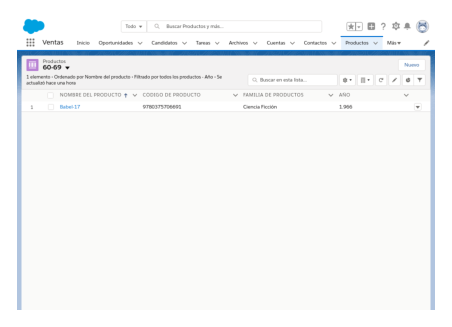
\includegraphics[width=1.0\textwidth]{graphics/productos.eps}
\caption{Interfaz gráfica para el módulo de productos.}
\label{productos_web}
\end{figure}

Para la evaluación de estas funcionalidades se realizarán las siguientes
evaluaciones:

\begin{itemize}
\item \textbf{Pruebas de aceptación}, para las funcionalidades de tipo CRUD en
    el gestor de productos, es decir, creación, visualización, modificación y
    eliminación.
\item \textbf{Pruebas funcionales}, para todos los elementos que están provistos
    por la misma interfaz de usuario.
\item \textbf{Pruebas de dominio}, para los cuatro formularios que maneja el
    gestor de productos, los cuales pueden verse en la figura \ref{productos_formularios}.
\item \textbf{Pruebas negativas}, para la evaluación de los mensajes de
    error provistos por este componente.
\end{itemize}

\begin{figure}
\centering
\begin{tikzpicture}[
    grow via three points={one child at (0.5,-0.7) and
    two children at (0.5,-0.7) and (0.5,-1.4)},
    edge from parent path={(\tikzparentnode.south) |- (\tikzchildnode.west)}]
    \node {Productos}
        child [missing] {}
        child { node {Crear producto}
            child { node {Nombre del producto (*)}}
            child { node {Activo}}
            child { node {Código de producto}}
            child { node {Familia de productos}}
            child { node {Descripción del producto}}
        }
        child [missing] {}
        child [missing] {}
        child [missing] {}
        child [missing] {}
        child [missing] {}
        child [missing] {}
        child { node {Crear entrada del catálogo de precios}
            child { node {Producto (*)}}
            child { node {Activo}}
            child { node {Lista de precios (*)}}
            child { node {Precio de la lista (*)}}
            child { node {Utilizar precio estándar}}
        }
        child [missing] {}
        child [missing] {}
        child [missing] {}
        child [missing] {}
        child [missing] {}
        child [missing] {}
        child { node {Agregar a lista de precios}
            child { node {Lista de precios (*)}}
            child { node {Divisa (*)}}
        }
        child [missing] {}
        child [missing] {}
        child [missing] {}
        child { node {Modificar entrada del catálogo de precios}
            child { node {Activo}}
            child { node {Precio de la lista}}
            child { node {Utilizar precio estándar}}
        };
\end{tikzpicture}
\caption{Formularios que componen el módulo de gestión de productos.}
\label{productos_formularios}
\end{figure}

\subsection{Listas de Precios}
En la figura \ref{listas_de_precios} pueden verse las funcionalidades
clasificadas desde la perspectiva de la interfaz de usuario, también se omitió
la sección de los controles de vista de lista.

\begin{figure}
\centering
\begin{tikzpicture}[
    grow via three points={one child at (0.5,-0.7) and
    two children at (0.5,-0.7) and (0.5,-1.4)},
    edge from parent path={(\tikzparentnode.south) |- (\tikzchildnode.west)}]
    \node {Listas de Precios}
        child [missing] {}
        child { node {Filtrar por: Vista de Lista}}
        child { node {Nuevo}}
        child { node {Buscar: Lista de precios}}
        child { node {Controles de Vista de Lista}
            child { node {\ldots}}
        }
        child [missing] {}
        child { node {Mostrar como}}
        child { node {Actualizar}}
        child { node {Modificar Lista}}
        child { node {Lista de Listas de Precios}
            child [missing] {}
            child { node {Ver: Lista de precios}
                child [missing] {}
                child { node {Modificar}}
                child { node {Eliminar}}
                child { node {Duplicar}}
                child { node {Relacionado}
                    child [missing] {}
                    child { node {Agregar productos}}
                    child { node {Ver: Producto}}
                    child { node {Modificar: Producto}}
                    child { node {Eliminar: Producto}}
                    child { node {Ver todos}}
                    child { node {Historial de lista de precios (Ver todos)}}
                }
                child [missing] {}
                child [missing] {}
                child [missing] {}
                child [missing] {}
                child [missing] {}
                child [missing] {}
                child [missing] {}
                child { node {Detalles}}
            }
            child [missing] {}
            child [missing] {}
            child [missing] {}
            child [missing] {}
            child [missing] {}
            child [missing] {}
            child [missing] {}
            child [missing] {}
            child [missing] {}
            child [missing] {}
            child [missing] {}
            child [missing] {}
            child [missing] {}
            child [missing] {}
            child { node {Modificar: Lista de Precios}}
            child { node {Eliminar: Lista de Precios}}
        };
\end{tikzpicture}
\caption{Funciones que componen el módulo de gestión de listas de precios.}
\label{listas_de_precios}
\end{figure}

Esta clasificación de las funciones se ubican en una vista de interfaz como
puede verse en la figura \ref{listas_de_precios_web}, vista principal para la
gestión de listas de precios en el servicio.

\begin{figure}
\centering
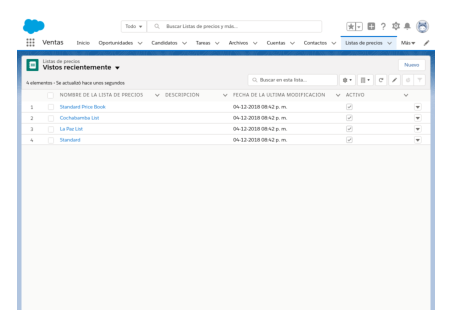
\includegraphics[width=1.0\textwidth]{graphics/listas_de_precios.eps}
\caption{Interfaz gráfica para el módulo de listas de precios.}
\label{listas_de_precios_web}
\end{figure}

Para la evaluación de estas funcionalidades se realizarán las siguientes
evaluaciones:

\begin{itemize}
\item \textbf{Pruebas de aceptación}, para las funcionalidades de tipo CRUD en
    el gestor de listas de precios, es decir, creación, visualización,
    modificación y eliminación.
\item \textbf{Pruebas funcionales}, para todos los elementos que están provistos
    por la misma interfaz de usuario.
\item \textbf{Pruebas de dominio}, para los dos formularios que maneja el
    gestor de productos, los cuales pueden verse en la figura \ref{listas_de_precios_formularios}.
\item \textbf{Pruebas negativas}, para la evaluación de los mensajes de error
    provistos por este componente.
\end{itemize}

\begin{figure}
\centering
\begin{tikzpicture}[
    grow via three points={one child at (0.5,-0.7) and
    two children at (0.5,-0.7) and (0.5,-1.4)},
    edge from parent path={(\tikzparentnode.south) |- (\tikzchildnode.west)}]
    \node {Listas de precios}
        child [missing] {}
        child { node {Crear lista de precios}
            child { node {Nombre de la lista de precios}}
            child { node {Activo}}
            child { node {Descripción}}
            child { node {Es lista de precios estándar}}
        }
        child [missing] {}
        child [missing] {}
        child [missing] {}
        child [missing] {}
        child [missing] {}
        child { node {Agregar productos}
            child { node {Buscar entrada de catálogos de precios}}
        };
\end{tikzpicture}
\caption{Formularios que componen el módulo de gestión de listas de precios.}
\label{listas_de_precios_formularios}
\end{figure}

\subsection{Controles de Vista de Lista}
En la figura \ref{vista_de_lista} pueden verse las funciones omitidas en los
diagramas anteriores relativas a los controles de vista, ambas equivalentes
entre si.

\begin{figure}
\centering
\begin{tikzpicture}[
    grow via three points={one child at (0.5,-0.7) and
    two children at (0.5,-0.7) and (0.5,-1.4)},
    edge from parent path={(\tikzparentnode.south) |- (\tikzchildnode.west)}]
    \node {Controles de Vista de Lista}
        child [missing] {}
        child { node {Duplicar}}
        child { node {Cambiar nombre}}
        child { node {Configuración de colaboración}}
        child { node {Modificar filtros de lista}
            child [missing] {}
            child { node {Ver/Modificar: Filtro}}
            child { node {Eliminar: Filtro}}
            child { node {Agregar Filtro}}
            child { node {Eliminar todos}}
            child { node {Agregar lógica de filtro}}
        }
        child [missing] {}
        child [missing] {}
        child [missing] {}
        child [missing] {}
        child [missing] {}
        child [missing] {}
        child [missing] {}
        child { node {Seleccionar los campos que se visualizaran}}
        child { node {Eliminar}}
        child { node {Restablecer anchuras de columna}};
\end{tikzpicture}
\caption{Funciones que componen el módulo de gestión de vistas de lista.}
\label{vista_de_lista}
\end{figure}

Para la evaluación de estas funcionalidades se realizarán las siguientes
evaluaciones:

\begin{itemize}
\item \textbf{Pruebas de aceptación}, para las funcionalidades de tipo CRUD en
    el gestor de vistas de lista, es decir, creación, visualización,
    modificación y eliminación.
\item \textbf{Pruebas funcionales}, para todos los elementos que están provistos
    por la misma interfaz de usuario.
\item \textbf{Pruebas de dominio}, para los seis formularios que maneja el
    gestor de vistas de lista, los cuales pueden verse en la figura
    \ref{vista_de_lista_formularios}.
\item \textbf{Pruebas negativas}, para la evaluación de los mensajes de
    error provistos por este componente.
\end{itemize}

\begin{figure}
\centering
\begin{tikzpicture}[
    grow via three points={one child at (0.5,-0.7) and
    two children at (0.5,-0.7) and (0.5,-1.4)},
    edge from parent path={(\tikzparentnode.south) |- (\tikzchildnode.west)}]
    \node {Vista de lista}
        child [missing] {}
        child { node {Nueva vista de lista}
            child { node {Nombre de la lista}}
            child { node {List API Name}}
            child { node {¿Quien ve esta vista de lista?}
                child { node {Solo yo puedo ver esta vista de lista}}
                child { node {Todos los usuarios pueden ver esta vista de lista}}
                child { node {Compartir vista de lista con grupos de usuarios}}
            }
        }
        child [missing] {}
        child [missing] {}
        child [missing] {}
        child [missing] {}
        child [missing] {}
        child [missing] {}
        child [missing] {}
        child { node {Cambiar nombre}
            child { node {Nombre de lista}}
            child { node {List API Name}}
        }
        child [missing] {}
        child [missing] {}
        child [missing] {}
        child { node {Configuración de colaboración}
            child { node {¿Quien ve esta vista de lista?}
                child { node {Solo yo puedo ver esta vista de lista}}
                child { node {Todos los usuarios pueden ver esta vista de lista}}
                child { node {Compartir vista de lista con grupos de usuarios}}
            }
        }
        child [missing] {}
        child [missing] {}
        child { node {Agregar filtro}
            child { node {Campo}}
            child { node {Operador}}
            child { node {Valor}}
        }
        child [missing] {}
        child [missing] {}
        child [missing] {}
        child [missing] {}
        child { node {Agregar lógica de filtro}
            child { node {Lógica de filtro}}
        }
        child [missing] {}
        child [missing] {}
        child { node {Seleccionar los campos que se visualizaran}
            child { node {Campos disponibles}}
            child { node {Campos visibles}}
        };
\end{tikzpicture}
\caption{Formularios que componen el módulo de gestión de vistas de listas.}
\label{vista_de_lista_formularios}
\end{figure}

\section{Técnicas de prueba}
Habiéndose definido los elementos del sistema, y los criterios bajo los que
estos deben ser evaluados. Ahora se pasará a describir las técnicas de prueba
que se utilizarán para cada elemento y criterio de calidad.

\subsection{Pruebas de aceptación}
La prueba de aceptación es una prueba formal que se realiza para determinar si
un sistema satisface sus criterios de aceptación: los criterios que debe cumplir
el sistema para que el cliente los acepte. Ayuda al cliente a determinar si
acepta o no el sistema\cite{Naik}.

Las pruebas de aceptación se realizaron para los tres componentes que comprenden
el alcance del proyecto, como el mínimo de las funcionalidades que se consideran
criticas, en este caso, las operaciones de creación, visualización, modificación
y eliminación de los elementos de cada componente.

Se crearon 55 casos de prueba, que pueden consultarse en los anexos de este
documento, siendo cada caso de prueba como el que se muestra en la figura
\ref{tc_acceptance}.

\begin{figure}
\centering
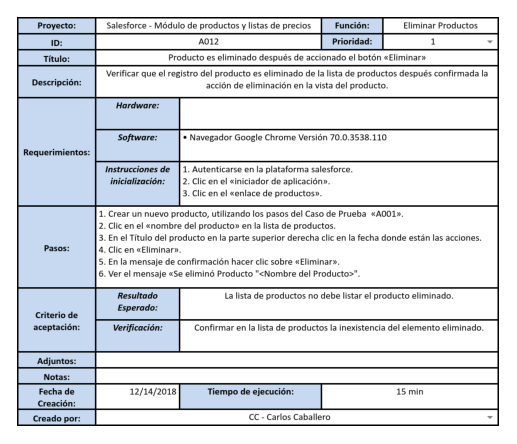
\includegraphics[width=1.0\textwidth]{graphics/tc1-acceptance.eps}
\caption{Caso de Prueba de Aceptación.}
\label{tc_acceptance}
\end{figure}

\subsection{Pruebas funcionales}
El software o sistema bajo prueba se ve como una «caja negra». La selección de
casos de prueba para pruebas funcionales se basa en el requisito o
especificación de diseño de la entidad de software bajo prueba. Ejemplos de
resultados esperados, algunas veces se llaman oráculos de prueba, incluyen
requisitos/especificaciones de diseño, valores calculados a mano y resultados
simulados. Las pruebas funcionales hacen hincapié en el comportamiento externo
de la entidad de software\cite{Luo}.

Las pruebas funcionales se realizaron para cada acción encontrada en la interfaz
de usuario, siendo barrido completamente cualquier operación disponible en los
componentes a evaluar.

Se crearon 144 casos de prueba, que pueden consultarse en los anexos de este
documento, siendo cada caso de prueba como el que se muestra en la figura
\ref{tc_functional}.

\begin{figure}
\centering
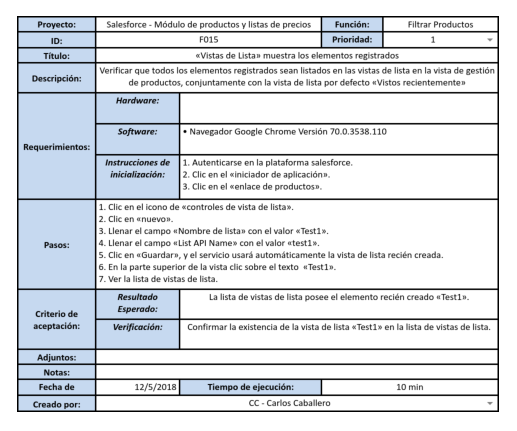
\includegraphics[width=1.0\textwidth]{graphics/tc2-functional.eps}
\caption{Caso de Prueba Funcional.}
\label{tc_functional}
\end{figure}

\subsection{Pruebas de dominio}
La prueba de dominio es una estrategia de muestreo estratificada para elegir
algunos casos de prueba de la infinidad de casos de prueba candidatos. La
estrategia tiene varios nombres, como la partición de equivalencia, el análisis
de límites y la partición de categorías.

La prueba de dominio es probablemente la más ampliamente descrita y una de las
técnicas de prueba de software más ampliamente practicadas. Algunos autores
restringen su consideración del alcance de esta técnica a variables de entrada
linealizables a funciones matemáticas. Una variable linealizable es aquella
cuyos valores se pueden asignar a una recta numérica. El análisis es más
sencillo y más obvio en estos casos\cite{Kaner}.

\subsection{Pruebas negativas}
La prueba negativa, comúnmente conocida como \emph{prueba de ruta de error} o
\emph{prueba de falla}, generalmente se realiza para garantizar la estabilidad
de la aplicación.

La prueba negativa es el proceso de aplicar tanta creatividad como sea posible y
validar la aplicación contra datos no válidos. Esto significa que su propósito
es verificar si los errores se muestran al usuario donde se supone que debe
hacerlo o si se está manejando un valor incorrecto con mayor gracia.

La fiabilidad funcional de la aplicación o el software solo se puede cuantificar
con escenarios negativos diseñados de manera efectiva. Las pruebas negativas no
solo apuntan a detectar fallas potenciales que podrían causar un impacto grave
en el consumo del servicio, sino que también pueden ser fundamentales para
determinar las condiciones bajo las cuales la aplicación puede fallar.
Finalmente, garantiza que haya suficiente validación de errores presente en el
software\cite{Nadig}.

Las pruebas negativas se centraron en los mensajes de errores que el sistema
envía y debe enviar según los mismos criterios del producto.

Se crearon 25 casos de prueba, que pueden consultarse en los anexos de este
documento, siendo cada caso de prueba como el que se muestra en la figura
\ref{tc_negative}.

\begin{figure}
\centering
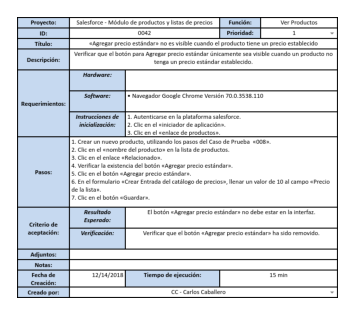
\includegraphics[width=1.0\textwidth]{graphics/tc3-negative.eps}
\caption{Caso de Prueba Negativa.}
\label{tc_negative}
\end{figure}

\subsection{Pruebas de compatibilidad}
La prueba de compatibilidad es una prueba no funcional realizada en la
aplicación para evaluar la compatibilidad de la aplicación en diferentes
entornos. En este caso sobre diferentes navegadores.

\subsection{Pruebas de localización}
El propósito de las pruebas de localización es asegurar que los errores no se
hayan introducido durante el proceso de traducción, que el contenido traducido
se muestre correctamente y que el producto localizado funcione como se espera
para el mercado objetivo. Probar sitios web para garantizar la adaptabilidad a
un lugar y una cultura en particular también es crucial para sugerir su
superioridad en el mercado objetivo\cite{Sampair}.

Aquí hay algunas áreas que examinamos durante esta prueba:

\begin{itemize}
\item Todos los recursos de localización están traducidos correctamente.
\item La compilación generada incluye todos los archivos necesarios.
\item La funcionalidad en la versión localizada es consistente con el producto de origen.
\item La pantalla localizada tiene el mismo número y tipo de elementos que el del producto de origen.
\item Todos los caracteres específicos del entorno local aparecen correctamente.
\item No hay palabras que pasen sobre los botones o se corten en la página.
\end{itemize}

\section{Criterios de calidad}
Se denomina criterio de calidad a cualquier requerimiento que define lo que el
producto debe ser.

Por lo general, los criterios de calidad parten de la combinación de las
necesidades reales y de las demandas de los clientes, con el conocimiento de las
ofertas y productos de organizaciones de la competencia y las posibilidades que
el fabricante posee para satisfacer esas necesidades y expectativas o para
procurar en la medida de lo posible y/o aconsejable\cite{Haaz}.

Se definieron los siguientes como criterios de calidad fundamentales para el
éxito del producto\cite{Fillottrani}.

\begin{description}
\item [Usabilidad] La usabilidad se refiere a la facilidad de operación del
    producto por parte de los usuarios, y se relaciona con el esfuerzo
    necesario para ser utilizado, y en la evaluación individual de tal uso, por
    parte de un conjunto especificado o implícito de usuarios.

    Entre algunos de los criterios que determinan este factor, están:

    \begin{itemize}
    \item \textbf{Entendimiento} que mide el esfuerzo del usuario en reconocer el
        concepto lógico del software y su aplicabilidad.
    \item \textbf{Aprendizaje} que mide el esfuerzo del usuario en aprender
        acerca del producto.
    \item \textbf{Operabilidad} que mide el esfuerzo del usuario en operar y
        controlar el sistema.
    \end{itemize}

\item [Compatibilidad] La compatibilidad del navegador determina el
    comportamiento del servicio en diferentes plataformas de navegación.

    Dado que cada navegador tiene su propia manera de mostrar y gestionar los
    contenidos de una página web. Por lo tanto, las páginas web deben diseñarse
    de tal manera que puedan ser compatibles con cada uno de los navegadores de
    uso común. Actualmente hay casi cien tipos diferentes de navegadores
    disponibles, lo que dificulta que los diseñadores / webmasters desarrollen
    sitios web con un comportamiento similar en múltiples plataformas. El
    estricto cumplimiento de las pautas de diseño puede cumplir con estos
    criterios hasta cierto nivel.

\item [Soportabilidad] La soportabilidad es la capacidad del sistema para
    proporcionar información útil para identificar y resolver problemas.

    El costo de mantener el atributo de compatibilidad es alto y el resultado
    solo es visible a gran escala. Sin embargo, con el crecimiento del equipo y
    el producto, este atributo se convierte en una de las claves\cite{Ashanin}.

\item [Localizabilidad] La localizabilidad es un proceso intermedio para
    verificar que una aplicación globalizada está lista para la localización.
    En una situación ideal, esta es solo una fase de garantía de calidad. Si se
    diseñó y desarrolló una aplicación con miras a la localización, esta fase
    consistirá principalmente en pruebas de localizabilidad. De lo contrario, es
    durante esta fase que se descubrirán y corregirán los errores en el código
    fuente que impiden la localización.

    La localizabilidad ayuda a garantizar que la localización no introduzca
    ningún defecto funcional en la aplicación\cite{Moura}.
\end{description}

